% entropy-2278906 
% Frank.Nielsen@acm.org
% Proofchecked camera April 14th 2023
%  LaTeX support: latex@mdpi.com 
%  For support, please attach all files needed for compiling as well as the log file, and specify your operating system, LaTeX version, and LaTeX editor.

%=================================================================
\documentclass[entropy,article,accept,oneauthor,pdftex,entropy]{Definitions/mdpi} 
 
\usepackage{graphicx,amssymb,amsmath,supertabular}
 
\graphicspath{{./Fig/}}
				
% For posting an early version of this manuscript as a preprint, you may use "preprints" as the journal and change "submit" to "accept". The document class line would be, e.g., \documentclass[preprints,article,accept,moreauthors,pdftex]{mdpi}. This is especially recommended for submission to arXiv, where line numbers should be removed before posting. For preprints.org, the editorial staff will make this change immediately prior to posting.

%--------------------
% Class Options:
%--------------------
%----------
% journal
%----------
% Choose between the following MDPI journals:
% acoustics, actuators, addictions, admsci, adolescents, aerospace, agriculture, agriengineering, agronomy, ai, algorithms, allergies, alloys, analytica, animals, antibiotics, antibodies, antioxidants, applbiosci, appliedchem, appliedmath, applmech, applmicrobiol, applnano, applsci, aquacj, architecture, arts, asc, asi, astronomy, atmosphere, atoms, audiolres, automation, axioms, bacteria, batteries, bdcc, behavsci, beverages, biochem, bioengineering, biologics, biology, biomass, biomechanics, biomed, biomedicines, biomedinformatics, biomimetics, biomolecules, biophysica, biosensors, biotech, birds, bloods, blsf, brainsci, breath, buildings, businesses, cancers, carbon, cardiogenetics, catalysts, cells, ceramics, challenges, chemengineering, chemistry, chemosensors, chemproc, children, chips, cimb, civileng, cleantechnol, climate, clinpract, clockssleep, cmd, coasts, coatings, colloids, colorants, commodities, compounds, computation, computers, condensedmatter, conservation, constrmater, cosmetics, covid, crops, cryptography, crystals, csmf, ctn, curroncol, currophthalmol, cyber, dairy, data, dentistry, dermato, dermatopathology, designs, diabetology, diagnostics, dietetics, digital, disabilities, diseases, diversity, dna, drones, dynamics, earth, ebj, ecologies, econometrics, economies, education, ejihpe, electricity, electrochem, electronicmat, electronics, encyclopedia, endocrines, energies, eng, engproc, ent, entomology, entropy, environments, environsciproc, epidemiologia, epigenomes, est, fermentation, fibers, fintech, fire, fishes, fluids, foods, forecasting, forensicsci, forests, foundations, fractalfract, fuels, futureinternet, futureparasites, futurepharmacol, futurephys, futuretransp, galaxies, games, gases, gastroent, gastrointestdisord, gels, genealogy, genes, geographies, geohazards, geomatics, geosciences, geotechnics, geriatrics, hazardousmatters, healthcare, hearts, hemato, heritage, highthroughput, histories, horticulturae, humanities, humans, hydrobiology, hydrogen, hydrology, hygiene, idr, ijerph, ijfs, ijgi, ijms, ijns, ijtm, ijtpp, immuno, informatics, information, infrastructures, inorganics, insects, instruments, inventions, iot, j, jal, jcdd, jcm, jcp, jcs, jdb, jeta, jfb, jfmk, jimaging, jintelligence, jlpea, jmmp, jmp, jmse, jne, jnt, jof, joitmc, jor, journalmedia, jox, jpm, jrfm, jsan, jtaer, jzbg, kidney, kidneydial, knowledge, land, languages, laws, life, liquids, literature, livers, logics, logistics, lubricants, lymphatics, machines, macromol, magnetism, magnetochemistry, make, marinedrugs, materials, materproc, mathematics, mca, measurements, medicina, medicines, medsci, membranes, merits, metabolites, metals, meteorology, methane, metrology, micro, microarrays, microbiolres, micromachines, microorganisms, microplastics, minerals, mining, modelling, molbank, molecules, mps, msf, mti, muscles, nanoenergyadv, nanomanufacturing, nanomaterials, ncrna, network, neuroglia, neurolint, neurosci, nitrogen, notspecified, nri, nursrep, nutraceuticals, nutrients, obesities, oceans, ohbm, onco, oncopathology, optics, oral, organics, organoids, osteology, oxygen, parasites, parasitologia, particles, pathogens, pathophysiology, pediatrrep, pharmaceuticals, pharmaceutics, pharmacoepidemiology, pharmacy, philosophies, photochem, photonics, phycology, physchem, physics, physiologia, plants, plasma, pollutants, polymers, polysaccharides, poultry, powders, preprints, proceedings, processes, prosthesis, proteomes, psf, psych, psychiatryint, psychoactives, publications, quantumrep, quaternary, qubs, radiation, reactions, recycling, regeneration, religions, remotesensing, reports, reprodmed, resources, rheumato, risks, robotics, ruminants, safety, sci, scipharm, seeds, sensors, separations, sexes, signals, sinusitis, skins, smartcities, sna, societies, socsci, software, soilsystems, solar, solids, sports, standards, stats, stresses, surfaces, surgeries, suschem, sustainability, symmetry, synbio, systems, taxonomy, technologies, telecom, test, textiles, thalassrep, thermo, tomography, tourismhosp, toxics, toxins, transplantology, transportation, traumacare, traumas, tropicalmed, universe, urbansci, uro, vaccines, vehicles, venereology, vetsci, vibration, viruses, vision, waste, water, wem, wevj, wind, women, world, youth, zoonoticdis 

%---------
% article
%---------
% The default type of manuscript is "article", but can be replaced by: 
% abstract, addendum, article, book, bookreview, briefreport, casereport, comment, commentary, communication, conferenceproceedings, correction, conferencereport, entry, expressionofconcern, extendedabstract, datadescriptor, editorial, essay, erratum, hypothesis, interestingimage, obituary, opinion, projectreport, reply, retraction, review, perspective, protocol, shortnote, studyprotocol, systematicreview, supfile, technicalnote, viewpoint, guidelines, registeredreport, tutorial
% supfile = supplementary materials

%----------
% submit
%----------
% The class option "submit" will be changed to "accept" by the Editorial Office when the paper is accepted. This will only make changes to the frontpage (e.g., the logo of the journal will get visible), the headings, and the copyright information. Also, line numbering will be removed. Journal info and pagination for accepted papers will also be assigned by the Editorial Office.

%------------------
% moreauthors
%------------------
% If there is only one author the class option oneauthor should be used. Otherwise use the class option moreauthors.

%---------
% pdftex
%---------
% The option pdftex is for use with pdfLaTeX. If eps figures are used, remove the option pdftex and use LaTeX and dvi2pdf.

%=================================================================
% MDPI internal commands
\firstpage{1} 
\makeatletter 
\setcounter{page}{\@firstpage} 
\makeatother
\pubvolume{1}
\issuenum{1}
\articlenumber{0}
\pubyear{2023}
\copyrightyear{2023}
\externaleditor{Academic Editor: Antonio M. Scarfone}
\datereceived{27 February 2023} 
\daterevised{6 April 2023} % Comment out if no revised date
\dateaccepted{12 April 2023 } 
\datepublished{ } 
%\datecorrected{} % For corrected papers: "Corrected: XXX" date in the original paper.
%\dateretracted{} % For corrected papers: "Retracted: XXX" date in the original paper.
\hreflink{https://doi.org/} % If needed use \linebreak
%\doinum{}
%\pdfoutput=1 % Uncommented for upload to arXiv.org

%=================================================================
% Add packages and commands here. The following packages are loaded in our class file: fontenc, inputenc, calc, indentfirst, fancyhdr, graphicx, epstopdf, lastpage, ifthen, lineno, float, amsmath, setspace, enumitem, mathpazo, booktabs, titlesec, etoolbox, tabto, xcolor, soul, multirow, microtype, tikz, totcount, changepage, attrib, upgreek, cleveref, amsthm, hyphenat, natbib, hyperref, footmisc, url, geometry, newfloat, caption

%=================================================================
%% Please use the following mathematics environments: Theorem, Lemma, Corollary, Proposition, Characterization, Property, Problem, Example, ExamplesandDefinitions, Hypothesis, Remark, Definition, Notation, Assumption
%% For proofs, please use the proof environment (the amsthm package is loaded by the MDPI class).

%=================================================================
% Full title of the paper (Capitalized)
\Title{A Simple Approximation Method for the Fisher--Rao Distance between Multivariate Normal Distributions}
 
 
% MDPI internal command: Title for citation in the left column
\TitleCitation{A Simple Approximation Method for the Fisher--Rao Distance between Multivariate Normal Distributions}

% Author Orchid ID: enter ID or remove command
\newcommand{\orcidauthorA}{0000-0001-5728-0726}  % Add \orcidA{} behind the author's name
%\newcommand{\orcidauthorB}{0000-0000-0000-000X} % Add \orcidB{} behind the author's name

% Authors, for the paper (add full first names)
\Author{{Frank Nielsen} %MDPI: Please carefully check the accuracy of names and affiliations.
 \orcidA{}}

%\longauthorlist{yes}

% MDPI internal command: Authors, for metadata in PDF
\AuthorNames{Frank Nielsen}

% MDPI internal command: Authors, for citation in the left column
\AuthorCitation{Nielsen, F.}
% If this is a Chicago style journal: Lastname, Firstname, Firstname Lastname, and Firstname Lastname.

% Affiliations / Addresses (Add [1] after \address if there is only one affiliation.)
\address[1]{Sony Computer Science Laboratories, Tokyo 141-0022, Japan; {frank.nielsen.x@gmail.com}}

% Contact information of the corresponding author
%\corres{Correspondence: e-mail@e-mail.com; Tel.: (optional; include country code; if there are multiple corresponding authors, add author initials) +xx-xxxx-xxx-xxxx (F.L.)}

% Current address and/or shared authorship
%\firstnote{Current address: Affiliation 3.} 
%\secondnote{These authors contributed equally to this work.}
% The commands \thirdnote{} till \eighthnote{} are available for further notes

%\simplesumm{} % Simple summary

%\conference{} % An extended version of a conference paper

% Abstract (Do not insert blank lines, i.e. \\) 

%\documentclass[11pt]{article}
%
%\usepackage[T1]{fontenc}


\def\Poincare{\mathrm{Poincar\acute{e}}}
\def\Hilbert{\mathrm{Hilbert}}
\def\Sym{\mathrm{Sym}}
\def\Log{{\mathrm{Log}}}
\def\barS{\bar{S}}
\def\det{\mathrm{det}}
\def\dsigma{\mathrm{d}\sigma}
\def\hatP{{\hat{P}}}
\def\Sinh{\mathrm{Sinh}}
\def\Cosh{\mathrm{Cosh}}
\def\sinh{\mathrm{sinh}}
\def\cosh{\mathrm{cosh}}
\def\arccsch{\mathrm{arccsch}}
\def\arccosh{\mathrm{arccosh}}
\def\arcsinh{\mathrm{arcsinh}}
\def\arctanh{\mathrm{arctanh}}
\def\bbP{\mathbb{P}}
\def\FR{\mathrm{FR}}
\def\SSPD{\mathrm{SSPD}}
\def\RieSEB{\mathrm{RieSEB}}
\def\calS{\mathcal{S}}
\def\calD{\mathcal{D}}
\def\supp{\mathrm{supp}}
\def\ball{\mathrm{ball}}
\def\calM{\mathcal{M}}
\def\calG{\mathcal{G}}
\def\SH{\mathbb{SH}}
\def\Sym{\mathrm{Sym}}
\def\dZ{\mathrm{d}Z}
\def\dY{\mathrm{d}Y}
\def\dP{\mathrm{d}P}
\def\dZbar{\mathrm{d}\bar Z}
\def\barZ{{\bar{Z}}}
\def\dtheta{\mathrm{d}\theta}
\def\SPC{\mathrm{SPC}}
\def\trace{\mathrm{trace}}
\def\proj{\mathrm{proj}}
\def\barN{{\overline{\mathcal{N}}}}
\def\dP{\mathrm{d}P}
\def\CO{\mathrm{CO}}
\def\bTheta{\bm{\Theta}}
\def\bEta{\mathbf{H}}
\def\rhoCO{\rho_{CO}}
\def\MVNSPD{C\&O\ }
\def\GL{\mathrm{GL}}
\def\KL{\mathrm{KL}}
\def\cN{\mathrm{cN}}
\def\Killing{\mathrm{Killing}}
\def\diag{\mathrm{diag}}
\def\CC{c}
\def\MVN{\mathrm{MVN}}
\def\SPD{\mathrm{SPD}}
\def\Aff{\mathrm{Aff}}
\def\bbR{\mathbb{R}}
\def\Fisher{\mathrm{Fisher}}
\def\vectortwo#1#2{{\left[\begin{array}{l}#1 \cr #2\end{array}\right]}}
\def\mattwotwo#1#2#3#4{{\left[\begin{array}{ll}#1 & #2\cr #3 & #4\end{array}\right]}}
\def\tr{\mathrm{tr}}
\def\barF{{\bar F}}
\def\bartheta{{\bar \theta}}
\def\bareta{{\bar \eta}}
\def\innerat#1#2#3{ {{\langle #2, #3\rangle}_{#1}} }
\def\inner#1#2{{\langle #1, #2\rangle}}
\def\calN{\mathcal{N}}
\def\Bi{\mathrm{Bi}}
\def\dx{\mathrm{d}x}
\def\dy{\mathrm{d}y}
\def\SPD{\mathrm{SPD}}
\def\calP{\mathcal{P}}
 \def\Rao{\mathrm{Rao}}
\def\Length{\mathrm{Length}}
\def\dt{\mathrm{d}t}
\def\rhoN{\rho_{\calN}}
\def\rhoP{\rho_P}
\def\mfdN{\mathscr{N}}
\def\mfdbarP{\bar\mathscr{P}}
\def\SS{\mathrm{SS}}
\def\dbeta{\mathrm{d}\beta}
\def\barLambda{{\bar\Lambda}}
\def\mfdP{\mathscr{P}}
\def\dim{\mathrm{dim}}
\def\Aff{\mathrm{Aff}}
\def\Var{\mathrm{Var}}
\def\vech{\mathrm{vech}}
\def\std{\mathrm{std}}
\def\barC{{\bar C}}
\def\barP{{\bar P}}
\def\dSigma{\mathrm{d}\Sigma}
\def\dmu{\mathrm{d}\mu}
\def\ds{\mathrm{d}s}
\def\st{\ :\ }
\def\bbR{\mathbb{R}}
\def\nablaG{\stackrel{\mathscr{G}}{\nabla}}
\def\nablaP{\stackrel{\mathscr{P}}{\nabla}}
\def\nablacG{\stackrel{\mathscr{G}_0}{\nabla}}
\def\Cov{\mathrm{Cov}}
\def\SL{\mathrm{SL}}
\def\SO{\mathrm{SO}}
\def\CandO{{C\&O}}

\abstract{We present a simple method to approximate the Fisher--Rao distance between multivariate normal distributions based on discretizing curves joining normal distributions and approximating the Fisher--Rao distances between successive nearby normal distributions on the curves by the square roots of their Jeffreys divergences. 
We consider experimentally the linear interpolation curves in the ordinary, natural, and expectation parameterizations of the normal distributions, and compare these curves with a curve derived from the Calvo and Oller's isometric embedding of the Fisher--Rao $d$-variate normal manifold into the cone of $(d+1)\times (d+1)$ symmetric positive–definite matrices.
We report on our experiments and assess the quality of our approximation technique by comparing the numerical approximations with both lower and upper bounds.
Finally, we present several information–geometric properties of Calvo and Oller's isometric embedding. 
}

\keyword{Fisher--Rao normal manifold;  symmetric positive–definite matrix cone; isometric embedding; information geometry; exponential family; elliptical distribution; maximal invariant}

\begin{document}

%%%
\section{Introduction}
%%%

%%
\subsection{The Fisher--Rao Normal~Manifold}
%%

Let $\Sym(d)$ be the set of $d\times d$ symmetric matrices with real entries and $\bbP(d)\subset\Sym(d)$ denote the set of symmetric positive–definite $d\times d$ matrices that forms a convex regular cone.
Let us denote by $\calN(d)=\{N(\mu,\Sigma) \st (\mu,\Sigma)\in\Lambda(d)=\bbR^d\times \bbP(d)\}$   the set of $d$-variate normal distributions, MultiVariate Normals or  MVNs for short, also called Gaussian distributions.
A MVN distribution $N(\mu,\Sigma)$ has probability density function (pdf) on the support $\bbR^d$:
$$
p_{\lambda=(\mu,\Sigma)}(x)= (2\pi)^{^\frac{d}{2}} |\Sigma|^{-\frac{1}{2}} \exp\left(-\frac{1}{2}(x-\mu)^\top\Sigma^{-1}(x-\mu)\right)
 ,\quad x\in\bbR^d,
$$
where $|M|=\det(M)$ denotes the determinant of matrix $M$.

The statistical model $\calN(d)$ is of dimension $m=\dim(\Lambda(d))=d+\frac{d(d+1)}{2}=\frac{d(d+3)}{2}$ since it is identifiable, i.e.,
there is a one-to-one correspondence $\lambda \leftrightarrow p_\lambda(x)$ between $\lambda\in\Lambda(d)$ and $N(\mu,\Sigma)\in\calN(d)$.
The statistical model $\calN(d)$ is said to be regular since the second-order derivatives $\frac{\partial^2 p_{\lambda}}{\partial\lambda_i\partial\lambda_j}$ and third-order derivatives $\frac{\partial^3 p_{\lambda}}{\partial\lambda_i\partial\lambda_j\partial\lambda_k}$ are smooth functions (defining the metric and cubic tensors in information geometry~\cite{IG-2016}), and~the set of first-order partial derivatives $\left\{\frac{\partial p_{\lambda}}{\partial\lambda_1},\ldots,\frac{\partial p_{\lambda}}{\partial\lambda_1}\right\}$ are linearly~independent.


Let $\Cov(X)$ denote the covariance of $X$ (variance when $X$ is scalar). 
A matrix $M$ is a semi-positive–definite if and only if $\forall x\not=0, x^\top M x\geq 0$.
The Fisher information matrix~\cite{calin2014geometric,IG-2016} (FIM) is the following symmetric semi-positive–definite matrix:
$$
I(\lambda)=\Cov[\nabla\log p_{\lambda}(x)]\succeq 0.
$$
{For} 
 regular statistical models $\{p_\lambda\}$, the~FIM  is positive–definite: $I(\lambda)\succ 0$, i.e.,~$\forall x\not=0, x^\top I(\lambda) x>0$. $M_1 \succ M_2$ denotes L\"owner partial ordering, i.e.,~the fact that $M_1-M_2$ is~positive–definite. 

The FIM is covariant under the reparameterization of the statistical model~\cite{calin2014geometric}.
That is, let $\theta(\lambda)$ be a new parameterization of the MVNs. Then we have:
$$
I_\theta(\lambda)=\left[\frac{\partial\lambda}{\partial\theta}\right]^\top\,\times\, I_\lambda(\lambda(\theta)) \,\times\,
 \left[\frac{\partial\lambda}{\partial\theta}\right].
$$
For example, we may parameterize univariate normal distributions by $\lambda=(\mu,\sigma^2)$ or $\theta=(\mu,\sigma)$.
We obtain the following Fisher information matrices for these parameterizations:
$$
I_\lambda(\lambda(\mu,\sigma))=\mattwotwo{\frac{1}{\sigma^2}}{0}{0}{\frac{1}{2\sigma^4}} \quad\mbox{and}\quad
I_\theta(\theta(\mu,\sigma))=\mattwotwo{\frac{1}{\sigma^2}}{0}{0}{\frac{1}{2\sigma^2}}.
$$
In higher dimensions, parameterization $\lambda=(\mu,\sigma^2)$ corresponds to the parameterization $(\mu,\Sigma)$ 
while parameterization $\theta=(\mu,L)$ where $\Sigma=LL^\top$ is the unique Cholesky decomposition with $L\in\GL(d)$, the~group of invertible $d\times d$ matrices. Another useful parameterization for optimization is the 
log–Cholesky parameterization~\cite{lin2019riemannian} ($\eta=(\mu,\log\sigma^2)\in\bbR^2$ for univariate normal distributions) which ensures that a gradient descent always stays in the domain. The~Fisher information matrix with respect to the log–Cholesky parameterization is 
$I_\eta(\eta(\mu,\sigma))=\mattwotwo{\frac{1}{\sigma^2}}{0}{0}{2}$ with $\eta(\mu,\sigma)\in\bbR^2$.


Since the statistical model $\calN(d)$ is identifiable and regular, the~Fisher information matrix can be written equivalently as follows~\cite{calin2014geometric,soen2021variance}:
\begin{eqnarray}
I(\mu,\Sigma)=\Cov[\nabla\log p_{(\mu,\Sigma)}] &=& E_{p_{(\mu,\Sigma)}}\left[\nabla\log p_{(\mu,\Sigma)}\nabla\log p_{(\mu,\Sigma)}^\top\right],\\
&=&-E_{p_{(\mu,\Sigma)}}\left[\nabla^2\log p_{(\mu,\Sigma)}\right]. \label{eq:FIM2}
\end{eqnarray}

For multivariate distributions parameterized by a $m$-dimensional vector (with $m=\frac{d(d+3)}{2}$)
$$
\theta=(\theta_1,\ldots,\theta_d,\theta_{d+1},\ldots,\theta_{m})\in\bbR^m,
$$
with $\mu=(\theta_1,\ldots,\theta_d)$ and $\Sigma(\theta)=\vech(\theta_{d+1},\ldots,\theta_{m})$ (inverse half-vectorization of matrices~\cite{barachant2013classification}), we have~\cite{Skovgaard-1981,Skovgaard-1984,malago2015information,herntier2022transversality}:
$$
I(\theta)=[I_{ij}(\theta)],\quad \mbox{with}\ 
I_{ij}(\theta)=
\left[\frac{\partial\mu}{\partial\theta_i}\right]^\top\Sigma^{-1}\frac{\partial\mu}{\partial\theta_j}
+\frac{1}{2}\tr\left(\Sigma^{-1}\frac{\partial\mu}{\partial\theta_i}\Sigma^{-1}\frac{\partial\mu}{\partial\theta_j} \right).
$$

By equipping the regular statistical model $\calN(d)$ with the Fisher information metric  
$$
g^\Fisher_\calN(\mu,\Sigma)=\Cov[\nabla\log p_{(\mu,\Sigma)}(x)]
$$
we obtain a Riemannian manifold $\calM=\calM_{\calN}$ called the Fisher--Rao Gaussian or normal manifold~\cite{Skovgaard-1981,Skovgaard-1984}.
The tangent space $T_N\calM$ is identified with the product space $\bbR^d\times\Sym(d)$. 
Let $\{\partial\mu,\partial\Sigma\}$ be a natural vector basis in $T_N\calM$, and~denote by $[v]$ and $[V]$ the vector components in that  natural basis.
%The vector components of the natural basis is
%$[\partial\mu]_{\lambda}=(1_d,0}$ and $[\partial\Sigma]_\lambda=\vectortwo{0}{I_d}$, where $1_d$ is the $d$-dimensional vector of $1$'s and $I_d$ the identity matrix of shape $d\times d$. 
We have
\begin{eqnarray*}
g^\Fisher_{(\mu,\Sigma)}((v_1,V_1),(v_2,V_2)) &=& \innerat{(\mu,\Sigma)}{(v_1,V_1)}{(v_2,V_2)},\\
&=& [v_1]^\top\Sigma^{-1}[v_2]+\frac{1}{2}\tr\left(\Sigma^{-1}[V_1]\Sigma^{-1}[V_2]\right).
\end{eqnarray*}


The induced Riemannian geodesic distance $\rho_\calN(\cdot,\cdot)$   is called the Rao distance~\cite{AtkinsonRao-1981} or the Fisher--Rao distance~\cite{Rao-1945,chen2021upper}:
\begin{equation}\label{eq:riedist}
\rho_\calN(N(\lambda_1),N(\lambda_2))=\inf_{\substack{c(t)\\ c(0)=p_{\lambda_1}\\ c(1)=p_{\lambda_2}}}  \, \left\{\Length(c)\right\},
\end{equation}
where the Riemannian length of any smooth curve $c(t)\in\calM$ is defined by
\begin{equation}
\Length(c)=\int_0^1 \sqrt{\innerat{c(t)}{\dot c(t)}{\dot c(t)}} \dt = \int_0^1 {\ds_\calN(t)} \dt = \int_0^1 \|\dot c(t)\|_{c(t)}\dt,
\end{equation}
{where} %Yes  it is correct. MDPI: Please check if this dot is correct here.
 $\dot{\ }=\frac{d}{\dt}$ denotes the derivative with respect to parameter $t$, $\ds_\calN(t)$ is the Riemannian length element of $(\calM,g_\calN^\Fisher)$ and $\|\cdot\|_{c(t)}=\sqrt{\innerat{c(t)}{\cdot}{\cdot}}$.
We also write $\rho_\calN(p_{\lambda_1},p_{\lambda_2})$ for $\rho_\calN(N(\lambda_1),N(\lambda_2))$.

The minimizing curve $c(t)=\gamma_\calN(p_{\lambda_1},p_{\lambda_2};t)$ of Equation~(\ref{eq:riedist}) is called the Fisher--Rao geodesic.
The Fisher--Rao geodesic is also an autoparallel curve~\cite{calin2014geometric} with respect to the Levi–Civita connection $\nabla^\Fisher_\calN$ induced by the Fisher metric $g^\Fisher_\calN$.
 

\begin{Remark}
If we consider the Riemannian manifold $(\calM,\beta g)$ for $\beta>0$ instead of $(\calM,g)$ then the length element $\ds$ is scaled by $\sqrt{\beta}$: $\ds_{\beta g}=\beta\, \ds_g$. It follows that the length of a curve $c$ becomes
$$
\Length_{\beta g}(c)=\sqrt{\beta}\, \Length_{g}(c).
$$
However, the~geodesics joining any two points $p_1$ and $p_2$ of $\calM$ are the same: $\gamma_{\beta g}(p_1,p_2;t)=\gamma_{g}(p_1,p_2;t)$ 
(with $\gamma_{g}(p_1,p_2;0)=p_1$ and 
$\gamma_{g}(p_1,p_2;1)=p_2$).
\end{Remark}


Historically, Hotelling~\cite{Hotelling-1930} first used this Fisher Riemannian geodesic distance in the late 1920s.
From the viewpoint of information geometry~\cite{IG-2016}, the~Fisher metric is the unique Markov invariant metric up to rescaling~\cite{cencov2000statistical,bauer2016uniqueness,fujiwara2022hommage}.
The counterpart to the Fisher metric on the compact manifold has been reported in~\cite{bruveris2019geometry}, proving its uniqueness under the action of the diffeomorphism group.
The Fisher--Rao distance has been used to design statistical hypothesis testing~\cite{burbea1989rao,SDPMVN-1990,rios1992rao,park1994distances}, to~measure the distance between the prior and posterior distributions in Bayesian statistics~\cite{gruber2008some}, in~clustering~\cite{strapasson2016clustering,le2019quantization},  in~signal processing~\cite{said2015texture,legrand2016evaluating,halder2018gradient,collas2022riemannian}, and~in deep learning~\cite{liang2019fisher}, just to mention a~few.

The squared line element induced by the Fisher metric of the multivariate normal family~\cite{Skovgaard-1981,Skovgaard-1984} is
\begin{eqnarray}
\ds^2_\calN(\mu,\Sigma)&=&\vectortwo{\dmu}{\dSigma}^\top\, I(\mu,\Sigma)\, \vectortwo{\dmu}{\dSigma},\\  \nonumber
&=& \dmu^\top \Sigma^{-1} \dmu + \frac{1}{2}\tr\left(\left(\Sigma^{-1}\dSigma\right)^2\right).
\end{eqnarray}

There are many ways to calculate the FIM/length element for multivariate normal distributions~\cite{Skovgaard-1984,herntier2022transversality}.
Let us give a simple approach based on the fact that the family $\calN(d)$ of normal distributions forms a regular exponential family~\cite{IG-MVN-1999}: 
$$
\calN(d)=\left\{p_{\theta(\lambda)}=\exp\left(\inner{\theta_v(\mu)}{x}+\inner{\theta_M(\Sigma)}{xx^\top}-F_\calN(\theta_v,\theta_M) \right)\right\},
$$
with $\theta(\lambda)=(\theta_v=(\Sigma^{-1}\mu,\theta_M=\frac{1}{2}\Sigma^{-1})$ the natural parameters and log-partition function (also called cumulant function)
$$
F_\calN(\theta) = \frac{1}{2}\left(d\log\pi-\log|\theta_M|+\frac{1}{2}\theta_v^\top\theta_M^{-1}\theta_v\right).
$$
The vector inner product is $\inner{v_1}{v_2}=v_1^\top v_2$, and~the matrix inner product is $\inner{M_1}{M_2}=\tr(M_1M_2^\top)$.
The exponential family is said to be regular when the natural parameter space is open.
Using Equation~(\ref{eq:FIM2}), it follows that the MVN FIM is 
$I_\theta(\theta)=-E[\nabla^2\log p_{\theta}]=\nabla^2 F(\theta)$.
This proves that the FIM is well-defined, i.e.,~$(I_\theta(\theta))_{ij}<\infty$.
As an exponential family~\cite{IG-2016}, we also have $I_\theta(\theta)=E[t(x)]$, where $t(x)=(x,xx^\top)$ is the sufficient statistic.
Thus, the Fisher metric is a Hessian metric~\cite{shima2007geometry}.
Let $F_\calN(\theta_v,\theta_M)=F_v(\theta_v)+F_M(\theta_M)$ with 
$F_v(\theta_v)=\frac{1}{2}\left(d\log\pi+\frac{1}{2}\theta_v^\top\theta_M^{-1}\theta_v\right)$
and
$F_M(\theta_M)=-\frac{1}{2} \log|\theta_M|$.
We obtain the following block-diagonal expression of the FIM:
$$
I(\theta(\lambda))=\nabla^2 F_\calN(\theta(\mu,\Sigma))=\mattwotwo{\Sigma^{-1}}{0}{0}{\frac{1}{2}\nabla^2_{\theta_M}\log|\frac{1}{2}\Sigma^{-1}|}.
$$
\textls[-35]{Therefore $\ds^2_\calN(\mu,\Sigma) = \ds^2_{v} + \ds^2_M$ with
$\ds^2_v(\mu)=\dmu^\top \Sigma^{-1} \dmu$ and 
$\ds^2_M(\Sigma)=\frac{1}{2}\tr\left(\left(\Sigma^{-1}\dSigma\right)^2\right)$.}
Let us note in passing that $\nabla^2_{\theta_M}\log|\theta_M|$ is a fourth order tensor~\cite{soen2021variance}.




The family $\calN(d)$ can also be considered to be an elliptical family~\cite{SDPElliptical-2002}, thus highlighting the affine-invariance property of the Fisher information metric.
That is, the~Fisher metric is invariant with respect to affine transformations~\cite{burbea1984informative}:
Let $(a,A)$ be an element of the affine group $\Aff(d)$ with $a\in\bbR^d$ and $A\in\GL(d)$.
The group identity element of $\Aff(d)$ is $e=(0,I)$ and the group operation {is} % No leave this . like that. it means action in mathematics. MDPI: Please check if the dot should be changed into the center dot in the following equation.
 $(a_1,A_1).(a_2,A_2)=(a_1+A_1a_2,A_1A_2)$ with inverse $(a,A)^{-1}=(-A^{-1}a,A^{-1})$).
Then we~have

\begin{Property}[Fisher–Rao affine invariance]\label{prop:aifr}
For all $A\in\GL(d), a\in\bbR^d$, we have
\begin{equation}
\rho_{\calN}(N(A\mu_1+a,A\Sigma_1A^\top),N(A\mu_2+a,A\Sigma_2A^\top))=\rho_{\calN}(N(\mu_1,\Sigma_1),N(\mu_2,\Sigma_2)).
\end{equation}
\end{Property}
This can be proven by checking that $\ds_\calN(\mu',\Sigma')=\ds_\calN(\mu,\Sigma)$ where $\mu'=A\mu+a$ and $\Sigma'=A\Sigma_2A^\top$.
It follows that we can reduce the calculation of the Fisher--Rao distance to a canonical case where one argument is
$N_\std=N(0,I)$, the~standard $d$-variate distribution:
\begin{eqnarray*}
\rho_{\calN}(N(\mu_1,\Sigma_1),N(\mu_2,\Sigma_2)) &=&
\rho_{\calN}\left(N_\std,N\left(\Sigma_1^{-\frac{1}{2}}(\mu_2-\mu_1),\Sigma_1^{-\frac{1}{2}}\Sigma_2\Sigma_1^{-\frac{1}{2}}\right)\right),\\
&=&
\rho_{\calN}\left(N\left(\Sigma_2^{-\frac{1}{2}}(\mu_1-\mu_2),\Sigma_2^{-\frac{1}{2}}\Sigma_1\Sigma_2^{-\frac{1}{2}}\right),N_\std\right),
\end{eqnarray*}
where $\Sigma^p$ is the fractional matrix power which can be calculated from the Singular Value Decomposition $O D O^\top$ of $\Sigma$ (where $O$ is an orthogonal matrix and $D=\diag(\lambda_1,\ldots,\lambda_d)$ a diagonal matrix):
$\Sigma^p=O D^p O^\top$ with $D^p=\diag(\lambda_1^p,\ldots, \lambda_d^p)$.

The~family of normal elliptical distributions can be obtained from the standard normal distribution by the action of the affine group~\cite{SDPElliptical-2002,chen2021upper} $\Aff(d)$:
$$
N(\mu,\Sigma)=(\mu,\Sigma^{\frac{1}{2}}).N_\std=N((\mu,\Sigma^{\frac{1}{2}}).(0,I)).
$$

 
%%%
\subsection{\textls[-25]{Fisher--Rao Distance between Normal Distributions: Some Subfamilies with Closed-Form~Formula}}
%%%
In general, the~Fisher–Rao distance $\rho_\calN(N_1,N_2)$ between two multivariate normal distributions $N_1$ and $N_2$ is not known in closed form~\cite{Eriksen-1986,FRGeodesicEll-1997,imai2011remarks,inoue2015group}, and~several lower and upper bounds~\cite{strapasson2015bounds}, and~numerical techniques such as the geodesic shooting~\cite{MVNGeodesicShooting-2014,GeodesicShooting-2016,barbaresco2019souriau} have been investigated. See~\cite{FRMVNReview-2020} for a recent review.
Unfortunately, the~geodesic shooting (GS) approach is time-consuming and numerically unstable for large Fisher--Rao distances~\cite{park1994distances,FRMVNReview-2020}. In~3D Diffusion Tensor Imaging (DTI), $3\times 3$ covariance matrices $\Sigma_{i,j,k}$ are stored a 3D grid locations $\mu_{i,j,k}$ thus generating 3D MVNs $N_{i,j,k}=N(\mu_{i,j,k},\Sigma_{i,j,k})$ with means $\mu_{i,j,k}$  regularly spaced to each others.
The Fisher--Rao distances can be calculated between an MVN $N_{i,j,k}$ and another MVN $N_{i',j',k'}$ in a neighborhood of $N_{i,j,k}$ (using $6$- or $26$-neighborhood) using geodesic shooting. For~larger Fisher--Rao distances between non-neighbors MVNs, we can use the shortest path distance using Dijkstra's algorithm~\cite{dijkstra2022note} on the graph induced by the MVNs with edges between adjacent MVNs weighted by their Fisher--Rao~distances.

The two main difficulties with calculating the Fisher--Rao distance~are 
\begin{enumerate}
\item \textls[-35]{ to know explicitly the expression of the Riemannian Fisher–Rao geodesic $\gamma_\calN^{\FR}(p_{\lambda_1},p_{\lambda_2};t)$ and}
\item  to integrate, in closed form, the length element $\ds_\calN$ along this Riemannian geodesic.
\end{enumerate}

Please note that the Fisher--Rao geodesics~\cite{IG-2016} $\gamma_\calN^{\mathrm{FR}}(p_{\lambda_1},p_{\lambda_2};t)$ are parameterized by constant speed (i.e., $\dot{\mu}(t)=\dot{\mu}(0)$ and $\dot\Sigma(t)=\dot\Sigma(0)$), or~equivalently parametrized using the  arc length:
$$
\rho_\calN\left(\gamma_\calN^{\mathrm{FR}}(p_{\lambda_1},p_{\lambda_2};s),\gamma_\calN^{\mathrm{FR}}(p_{\lambda_1},p_{\lambda_2};t)\right)
=
|s-t|\, \rho_\calN(p_{\lambda_1},p_{\lambda_2}),\quad \forall s,t\in[0,1].
$$

However, in~several special cases, the~Fisher–Rao distance between normal distributions belonging to restricted subsets of $\calN$ is~known.

Three such prominent cases are (see~\cite{FRMVNReview-2020}  for other cases)
\begin{enumerate}
\item  when the normal distributions are univariate ($d=1$),  

\item  when we consider the set
$\calN_\mu=\{N(\mu,\Sigma)\st \Sigma\in\calP(d)\}\subset\calM_{\calN}$ of normal distributions sharing the same mean $\mu$ (with the embedded submanifold $\calS_\mu\in\calM$), and~

\item  when  we consider the set
$\calN_\Sigma=\{N(\mu,\Sigma)\st \Sigma\in\calP(d)\}\subset\calN$ of normal distributions sharing the same covariance matrix $\Sigma$ 
(with the corresponding embedded submanifold $\calS_\Sigma\in\calM$).
\end{enumerate}

Let us report the formula of the Fisher--Rao distance in these three cases:


\begin{itemize}

\item
In the univariate case $\calN(1)$, the~Fisher--Rao distance between $N_1=N(\mu_1,\sigma_1^2)$ and $N_2=N(\mu_2,\sigma_2^2)$ can be derived from the hyperbolic distance~\cite{anderson2006hyperbolic} expressed in the Poincar\'e upper space since we have
$$
\ds^2_\calN=g_{(\mu,\sigma)}(\dmu,\dsigma)=\frac{\dmu^2+2\dsigma^2}{\sigma^2}=2 \frac{\left(\frac{\dmu}{\sqrt{2}}\right)^2+\dsigma^2}{\sigma^2}
=2 \frac{\dx^2+\dy^2}{y^2}=\ds^2_{\Poincare},
$$
where $x=\frac{\mu}{\sqrt{2}}$ and $y=\sigma$.
It follows that 
$$
\rho_\calN(N_1,N_2)=
\sqrt{2}\, \rho_{\Poincare}((x_1,y_1),(x_2,y_2))=
\sqrt{2}\, \rho_{\Poincare}\left(\left(\frac{\mu_1}{\sqrt{2}},\sigma_1\right),\left(\frac{\mu_2}{\sqrt{2}},\sigma_2\right)\right).
$$
Thus, we have the following expression for the Fisher--Rao distance between univariate normal distributions:
\begin{equation}\label{eq:FR1D}
\rho_{\calN}(N_1,N_2)=\sqrt{2}\log \left(\frac{1+\Delta(\mu_1,\sigma_1;\mu_2,\sigma_2)}{1-\Delta(\mu_1,\sigma_1;\mu_2,\sigma_2)}\right)
,
\end{equation}
with
\begin{equation}
\Delta(a,b;c,d)=\sqrt{\frac{(c-a)^2+2(d-b)^2}{(c-a)^2+2(d+b)^2}}, \quad (a,b,c,d)\in\bbR^4\backslash\{0\}.
\end{equation}
In particular, we~have
\begin{itemize}
\item $\Delta(a,b;a,d)=\left|\frac{d-b}{d+b}\right|$ when $a=c$ (same mean),  
\item $\Delta(a,b;c,b)=\sqrt{\frac{1}{1+8\frac{b^2}{(c-a)^2}}}$ when $b=d$ (same variance), 
\item $\Delta(0,1;c,d)=\sqrt{\frac{c^2+2(d-1)^2}{c^2+2(d+1)^2}}$  when $a=0$ and $b=1$ (standard normal).
\end{itemize}
In 1D, the~affine-invariance property (Property~\ref{prop:aifr}) extends to function $\Delta$ as follows:
$$
\Delta(\mu_1,\sigma_1;\mu_2,\sigma_2)=\Delta\left(0,1;\frac{\mu_2-\mu_1}{\sigma_1},\frac{\sigma_2}{\sigma_1}\right)
=\Delta\left(\frac{\mu_1-\mu_2}{\sigma_2},\frac{\sigma_1}{\sigma_2};0,1\right).
$$

Using one of the many identities between inverse hyperbolic functions (e.g., arctanh, arccosh, arcsinh), we can obtain an equivalent formula for Equation~(\ref{eq:FR1D}).
For example, since $\arctanh(u):=\frac{1}{2}\log\left(\frac{1+u}{1-u}\right)$ for $0<u<1$, we have equivalently:
\begin{equation}
\rho_{\calN}(N_1,N_2)= 2\sqrt{2}\,\arctanh(\Delta(\mu_1,\sigma_1;\mu_2,\sigma_2)).
\end{equation}

The Fisher–Rao geodesics are semi-ellipses with centers located on the $x$-axis.
See Appendix~\ref{sec:geo1d} for the parametric equations of Fisher–Rao geodesics between univariate normal distributions.
Figure~\ref{fig:normal1d} displays four univariate normal distributions with their pairwise geodesics and Fisher–Rao~distances.


Using the identity $\arctanh\left(\frac{u^2-1}{u^2+1}\right)=\arccosh\left(\frac{1+u^2}{2u}\right)$ with 
$\arccosh(x):=\log(x+\sqrt{x^2-1})$, we also have
$$
\rho_{\calN}(N_1,N_2)=2\sqrt{2}\,\arccosh\left(\frac{1}{\sqrt{(1-\Delta(\mu_1,\sigma_1;\mu_2,\sigma_2))(1+\Delta(\mu_1,\sigma_1;\mu_2,\sigma_2))}}\right),
$$
Since the inverse hyperbolic cosecant (CSC) function is defined by $\arccsch(u):=\arccosh(1/u)$, we further obtain
$$
\rho_{\calN}(N_1,N_2)= 2\sqrt{2}\,\arccsch\left(\sqrt{(1-\Delta(\mu_1,\sigma_1;\mu_2,\sigma_2))(1+\Delta(\mu_1,\sigma_1;\mu_2,\sigma_2))}\right),
$$
We can also write
$$
\rho_{\calN}(N_1,N_2)=\sqrt{2}\,\arccosh\left(1+\frac{(\mu_2-\mu_1)^2+2(\sigma_2-\sigma_1)^2}{4\sigma_1\sigma_2}\right)
$$

Thus, using the many-conversions formula between inverse hyperbolic functions, we obtain many equivalent different formulas of the Fisher--Rao distance, which are used in the~literature.



\begin{figure}[H]

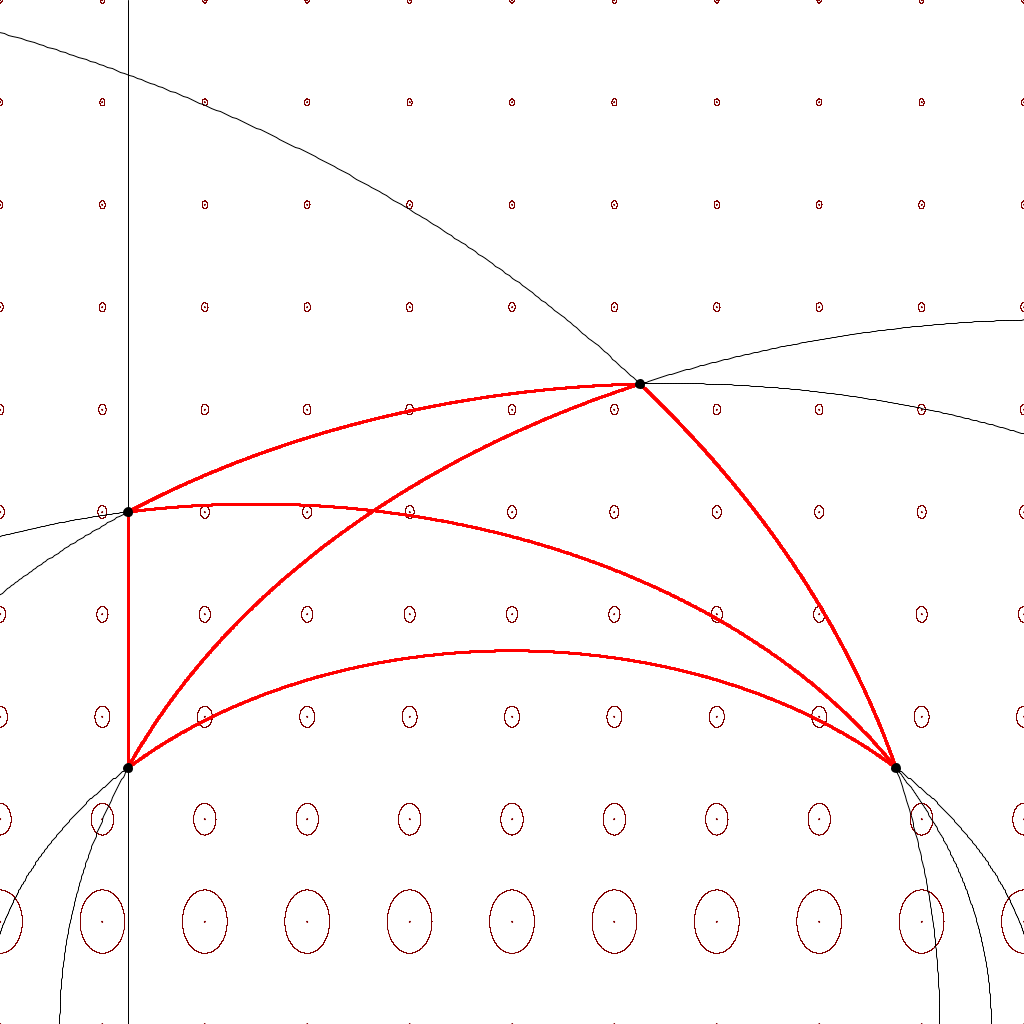
\includegraphics[width=0.35\textwidth]{Fig-Example4normals.png}
%
\caption{Four univariate normal distributions 
$N_1=N(0,1)$, $N_2=N(3,1)$, $N_3=N(2,2.5)$, $N_4=N(0,2)$, and~their pairwise full geodesics in gray and geodesics linking them in red.
The Fisher--Rao distances {are} %Yes, correct. it means we truncated more precisions. MDPI: Please check if \ldots is correct here, please check if it should be ,\ldots, here, e.g., 2.6124,\ldots,.
 $\rho_\calN(N_1,N_2)=2.6124\ldots$, $\rho_\calN(N_3,N_4)=0.9317\ldots$,
$\rho_\calN(N_1,N_4)=0.9803\ldots$, $\rho_\calN(N_2,N_3)=1.4225\ldots$
$\rho_\calN(N_2,N_4)=2.1362\ldots$, and~$\rho_\calN(N_1,N_3)=1.7334\ldots$
The ellipses are Tissot indicatrices, which visualize the metric tensor $g_\calN^\Fisher$ at grid positions.
 \label{fig:normal1d}}
\end{figure}






\item In the second case, the~Fisher--Rao distance between $N_1=N(\mu,\Sigma_1)$ and $N_2=N(\mu,\Sigma_2)$ has been reported in~\cite{siegel2014symplectic,DoubleCone-James-1973,Skovgaard-1981,Skovgaard-1984,wells2020fisher}:
\begin{eqnarray}
\rho_{\calN_\mu}(N_1,N_2)&=& \sqrt{\frac{1}{2} \sum_{i=1}^d \log^2 \lambda_i(\Sigma_1^{-1}\Sigma_2)},\\ \label{eq:RaoCMVN}
&=&\rho_{\calN_{\mu}}(\Sigma_1,\Sigma_2),
\end{eqnarray}
where $\lambda_i(M)$ denotes the $i$-th generalized largest eigenvalue of matrix $M$, where the generalized eigenvalues are solutions of the equation $|\Sigma_1-\lambda\Sigma_2|=0$.
Let us notice that  $\rho_{\calN_\mu}((\mu,\Sigma_1),(\mu,\Sigma_2))=\rho_{\calN_\mu}((\mu,\Sigma_1^{-1}),(\mu,\Sigma_2^{-1}))$
 since $\lambda_i(\Sigma_2^{-1}\Sigma_1)=\frac{1}{\lambda_i(\Sigma_1^{-1}\Sigma_2)}$ and 
 $\log^2 \lambda_i(\Sigma_2^{-1}\Sigma_1)=(-\log \lambda_i(\Sigma_1^{-1}\Sigma_2))^2=\log^2 \lambda_i(\Sigma_1^{-1}\Sigma_2)$.
Matrix $\Sigma_1^{-1}\Sigma_2$ may not be SPD and thus the $\lambda_i$'s are generalized eigenvalues.
 We may consider instead the SPD matrix $\Sigma_1^{-\frac{1}{2}}\Sigma_2\Sigma_1^{-\frac{1}{2}}$ which is SPD and such that $\lambda_i(\Sigma_1^{-1}\Sigma_2)=\lambda_i(\Sigma_1^{-\frac{1}{2}}\Sigma_2\Sigma_1^{-\frac{1}{2}})$.
The Fisher--Rao distance of Equation~(\ref{eq:RaoCMVN}) can be equivalently written~\cite{calvo1991explicit} as
$$
\rho_{\calN_\mu}(N_1,N_2)=\frac{1}{\sqrt{2}}\, \left\|\Log\left(\Sigma_1^{-\frac{1}{2}}\Sigma_2\Sigma_1^{-\frac{1}{2}}\right)\right\|_F,
$$
\textls[-35]{where $\Log(M)$ is the matrix logarithm (unique when $M$ is SPD) and $\|M\|_F=\sqrt{\sum_{i,j} M_{i,j}^2}=\sqrt{\tr(MM^\top)}$ is the matrix Fr\"obenius norm.
This metric distance between SPD matrices although first studied by Siegel~\cite{siegel2014symplectic} in 1964 was rediscovered and analyzed recently in~\cite{forstner2003metric} (2003).
Let $\rho_\SPD(P_1,P_2)=\sqrt{  \sum_{i=1}^d \log^2 \lambda_i(P_1^{-1}P_2)}$ so that $\rho_{\calN_\mu}(N(\mu,P_1),N(\mu,P_2))=\frac{1}{\sqrt{2}}\, \rho_\SPD(P_1,P_2)$.}

The Riemannian SPD distance $\rho_\SPD$ enjoys the following well-known invariance properties:

\begin{itemize} 

\item Invariance by congruence transformation:
\begin{equation}\label{eq:spdconginvar}
\forall X\in\GL(d),\quad \rho_\SPD(XP_1X^\top,XP_2X^\top)=\rho_\SPD(P_1,P_2),
\end{equation}

\item Invariance by inversion:
$$
\forall P_1,P_2\in\bbP(d),\quad  \rho(P_1^{-1},P_2^{-1})=\rho_\SPD(P_1,P_2).
$$
Let $P_1=L_1L_1^\top$ be the Cholesky decomposition (unique when $P_1\succ 0$). 
Then apply the congruence invariance for $X=L_1^{-1}$:

\begin{adjustwidth}{-\extralength}{0cm}
\centering %% If there is a figure in wide page, please release command \centering
\begin{equation}
\rho_\SPD(P_1,P_2)=\rho_\SPD(L_1^{-1}P_1(L_1^{-1})^\top,L_1^{-1}P_2(L_1^{-1})^\top)=\rho_\SPD(I,L_1^{-1}P_2(L_1^{-1})^\top).
\end{equation}
\end{adjustwidth}
We can also consider the factorization $P_1=S_1S_1$ where $S_1=P_1^{\frac{1}{2}}$ is the unique symmetric square root matrix~\cite{dolcetti2020real}.
Then we have
$$
\rho_\SPD(P_1,P_2)=\rho_\SPD(S_1^{-1}P_1(S_1^{-1})^\top,S_1^{-1}P_2(S_1^{-1})^\top)=\rho_\SPD(I,S_1^{-1}P_2(S_1^{-1})^\top).
$$
\end{itemize}

 

\item The Fisher--Rao distance between $N_1=N(\mu_1,\Sigma)$ and $N_2=N(\mu_2,\Sigma)$ has been reported in closed form~\cite{FRMVNReview-2020} (Proposition~3). The~method is described with full details in Appendix~\ref{sec:BFRsamecovar}.
We  present a simpler  scheme based on the inverse $\Sigma^{-\frac{1}{2}}$ of the symmetric square root factorization~\cite{dolcetti2020real} of $\Sigma=\Sigma^{\frac{1}{2}}\Sigma^{\frac{1}{2}}$ (ith $(\Sigma^{-\frac{1}{2}})^\top=\Sigma^{-\frac{1}{2}}$). Let us use the affine-invariance property of the Fisher–Rao distance under the affine transformation $\Sigma^{-\frac{1}{2}}$ and then apply affine invariance under translation as follows:
\begin{eqnarray*}
\rho_\calN(N(\mu_1,\Sigma),N(\mu_2,\Sigma)) &=&
 \rho_\calN(N(\Sigma^{-\frac{1}{2}}\mu_1,\Sigma^{-\frac{1}{2}}\Sigma\Sigma^{-\frac{1}{2}}),N(\Sigma^{-\frac{1}{2}}\mu_2,\Sigma^{-\frac{1}{2}}\Sigma\Sigma^{-\frac{1}{2}})),\\
&=& \rho_\calN(N(0,I),N(\Sigma^{-\frac{1}{2}}(\mu_2-\mu_1),I)),\\
&=& \rho_\calN(N(0,1),N(\|\Sigma^{-\frac{1}{2}}(\mu_2-\mu_1)\|_2,1)).
\end{eqnarray*}
The right-hand side Fisher–Rao distance is computed from Equation~(\ref{eq:FR1D}) and justified by the method~\cite{FRMVNReview-2020} (Proposition~3) described in  Appendix~\ref{sec:BFRsamecovar} using a rotation matrix $R$ with $RR^\top=I$ so that 
\begin{eqnarray*}
\rho_\calN(N(0,I),N(\Sigma^{-\frac{1}{2}}(\mu_2-\mu_1),I))&=&\rho_\calN(N(0,I),N(R \Sigma^{-\frac{1}{2}}(\mu_2-\mu_1),RIR^\top)),\\
&=& \rho_\calN(N(0,I),\|\Sigma^{-\frac{1}{2}}(\mu_2-\mu_1)\|_2,I)).
\end{eqnarray*}
Then we apply the formula of Equation~(23) of~\cite{FRMVNReview-2020}.
Section~\ref{sec:FRsamecovar} shall report a simpler closed-form formula by proving that the Fisher–Rao distance between $N(\mu_1,\Sigma)$ and $N(\mu_2,\Sigma)$ is a scalar function of their Mahalanobis distance~\cite{mahalanobis1936generalised} using the algebraic method of maximal invariants~\cite{eaton1989group}.
\end{itemize}

%\end{paracol}\end{document}

 

%%%
\subsection{Fisher–Rao Distance:  Totally versus Non-Totally Geodesic~Submanifolds}\label{sec:submfd}
%%%
Consider $\calN'=\{N(\lambda) \st\lambda'\in\Lambda'\}\subset\calN$ a statistical submodel of the MVN statistical model $\calN$.
Using the Fisher information matrix $I_{\lambda'}(\lambda')$, we obtain the intrinsic Fisher–Rao manifold $\calM'=\calM_{\calN'}$.
We may also consider $\calM'$ to be an embedded submanifold of $\calM$. 
 Let us write $\calS'=\calS_{\calN'}\subset\calM$ the embedded~submanifold.

A totally geodesic submanifold $\calS'\subset\calM$ is such that the geodesics $\gamma_{\calM'}(N_1',N_2';t)$ fully stay in $\calM'$ for any pair of points $N_1',N_2'\in\calN'$.
For example, the~submanifold $\calM_\mu=\{N(\mu,\Sigma)\st \Sigma\in\bbP(d)\}\subset\calM$ of MVNs with fixed mean $\mu$ is a totally geodesic submanifold~\cite{godinho2012introduction} of $\calM$ but the submanifold $\calM_\Sigma=\{N(\mu,\Sigma)\st \mu\in\bbR^d\}\subset\calM$ of MVNs sharing the same  
covariance matrix $\Sigma$ is not totally geodesic. 
When an embedded submanifold $\calS\subset\calM$ is totally geodesic, we always 
have $\rho_{\calM}(N_1,N_2)=\rho_{\calS}(N_1,N_2)$.
Thus, we have $\rho_\calN(N(\mu,\Sigma_1),N(\mu,\Sigma_2))=\rho_\SPD(\Sigma_1,\Sigma_2)$.
However, when an embedded submanifold $\calS\subset\calM$ is not totally geodesic, we have $\rho_{\calM}(N_1,N_2)\leq \rho_{\calS}(N_1,N_2)$ because the Riemannian geodesic length in $\calS$ is necessarily longer or equal than the Riemannian geodesic length in $\calM$.
The merit to consider submanifolds is to be able to calculate in closed form the Fisher–Rao distance which may then provide an upper bound on the Fisher–Rao distance for the full statistical model.
For example, consider $N_1=N(\mu_1,\Sigma)$ and $N_2=N(\mu_2,\Sigma)$ in $\calM_\Sigma$, a~non-totally geodesic submanifold.
The Rao distance between $N_1$ and $N_2$ in $\calM$ is upper bounded by the Riemannian distance in $\calM_\Sigma$ 
(with line element $\ds_\Sigma^2=\dmu^\top\Sigma^{-1}\dmu$) which corresponds to the Mahalanobis distance~\cite{mahalanobis1936generalised,AtkinsonRao-1981} $\Delta_\Sigma(\mu_1,\mu_2)$:
\begin{equation}
\rho_{\calM_\mu}(N_1,N_2)\leq  \Delta_\Sigma(\mu_1,\mu_2):=\sqrt{(\mu_2-\mu_1)^\top \Sigma^{-1} (\mu_2-\mu_1)}.
\end{equation}
 
The Mahalanobis distance can be interpreted as the Euclidean distance $D_E(p,q)=\Delta_I(p,q)=\sqrt{(p-q)^\top (p-q)}$ (where $I$ denotes the identity matrix) after an affine transformation: Let $\Sigma=LL^\top=U^\top U$ be the Cholesky decomposition of $\Sigma\gg 0$ with $L$ a lower triangular matrix or $U=L^\top$ an upper triangular matrix. Then we have 
\begin{eqnarray*}
\Delta_\Sigma(\mu_1,\mu_2)&=&\sqrt{(\mu_2-\mu_1)^\top (L^\top)^{-1} L^{-1} (\mu_2-\mu_1)},\\
&=&\|\Sigma^{-\frac{1}{2}}(\mu_2-\mu_1)\|_2,\\
&=&\Delta_I(L^{-1}\mu_1,L^{-1}\mu_2)=D_E(L^{-1}\mu_1,L^{-1}\mu_2),
\end{eqnarray*}
where $\|\cdot\|_2$ denotes the vector $\ell_2$-norm.

The Rao distance $\rho_\Sigma$ of Equation~(\ref{eq:FRSigma}) between two MVNs with fixed covariance matrix emanates from the property that the submanifold 
$\calM_{[v],\Sigma}=\{N(a v,\Sigma) \st a\in\bbR\}$ is totally geodesic~\cite{strapasson2016totally}.

Let us emphasize that for a submanifold $\calS\subset\calM$ to be totally geodesic or not depend on the underlying metric in $\calM$. 
The same subset $\calN'\subset\calN$ with $\calN$ equipped with two different metrics $g_1$ and $g_2$ can be totally geodesic regarding $g_1$ and non-totally geodesic regarding $g_2$. See Remark~\ref{rk:secondco} for such an~example.



In general, using the triangle inequality of the Riemannian metric distance $\rho_\calN$, we can upper bound $\rho_\calN(N_1,N_2)$ with $N_1=(\mu_1,\Sigma_1)$ and $N_1=(\mu_2,\Sigma_2)$  as follows:
\begin{eqnarray*}
\rho_\calN(N_1,N_2)&\leq& \rho_{\calM_{\mu_1}}(N_1,N_{12})+\rho_{\calM_{\Sigma_2}}(N_{12},N_2),\\
&\leq& \rho_{\calM_{\Sigma_1}}(N_1,N_{21})+\rho_{\calM_{\mu_2}}(N_{21},N_2),
\end{eqnarray*}
where $N_{12}=(\mu_1,\Sigma_2)$ and $N_{21}=N(\mu_2,\Sigma_1)$.
See Figure~\ref{fig:totallynottotally} for an illustration of the Fisher--Rao geodesic triangle $\triangle N_1,N_2,N_{12}$.
Furthermore, since $\rho_{\calN_{\Sigma_1}}(N_1,N_{21})\leq\Delta_{\Sigma_1}(\mu_1,\mu_2)$ and 
$\rho_{\calN_{\Sigma_2}}(N_{12},N_2)\leq \Delta_{\Sigma_2}(\mu_1,\mu_2)$, we obtain the following upper bound on the Rao distance between MVNs:
\begin{equation}\label{eq:UBMah}
\rho_{\mathcal{N}}(N_1,N_2)\leq \rho_{\mathcal{P}}(\Sigma_1,\Sigma_2)+\min\{\Delta_{\Sigma_1}(\mu_1,\mu_2),\Delta_{\Sigma_2}(\mu_1,\mu_2)\}.
\end{equation}
See also~\cite{chen2022multisensor}. 

\begin{figure}[H]

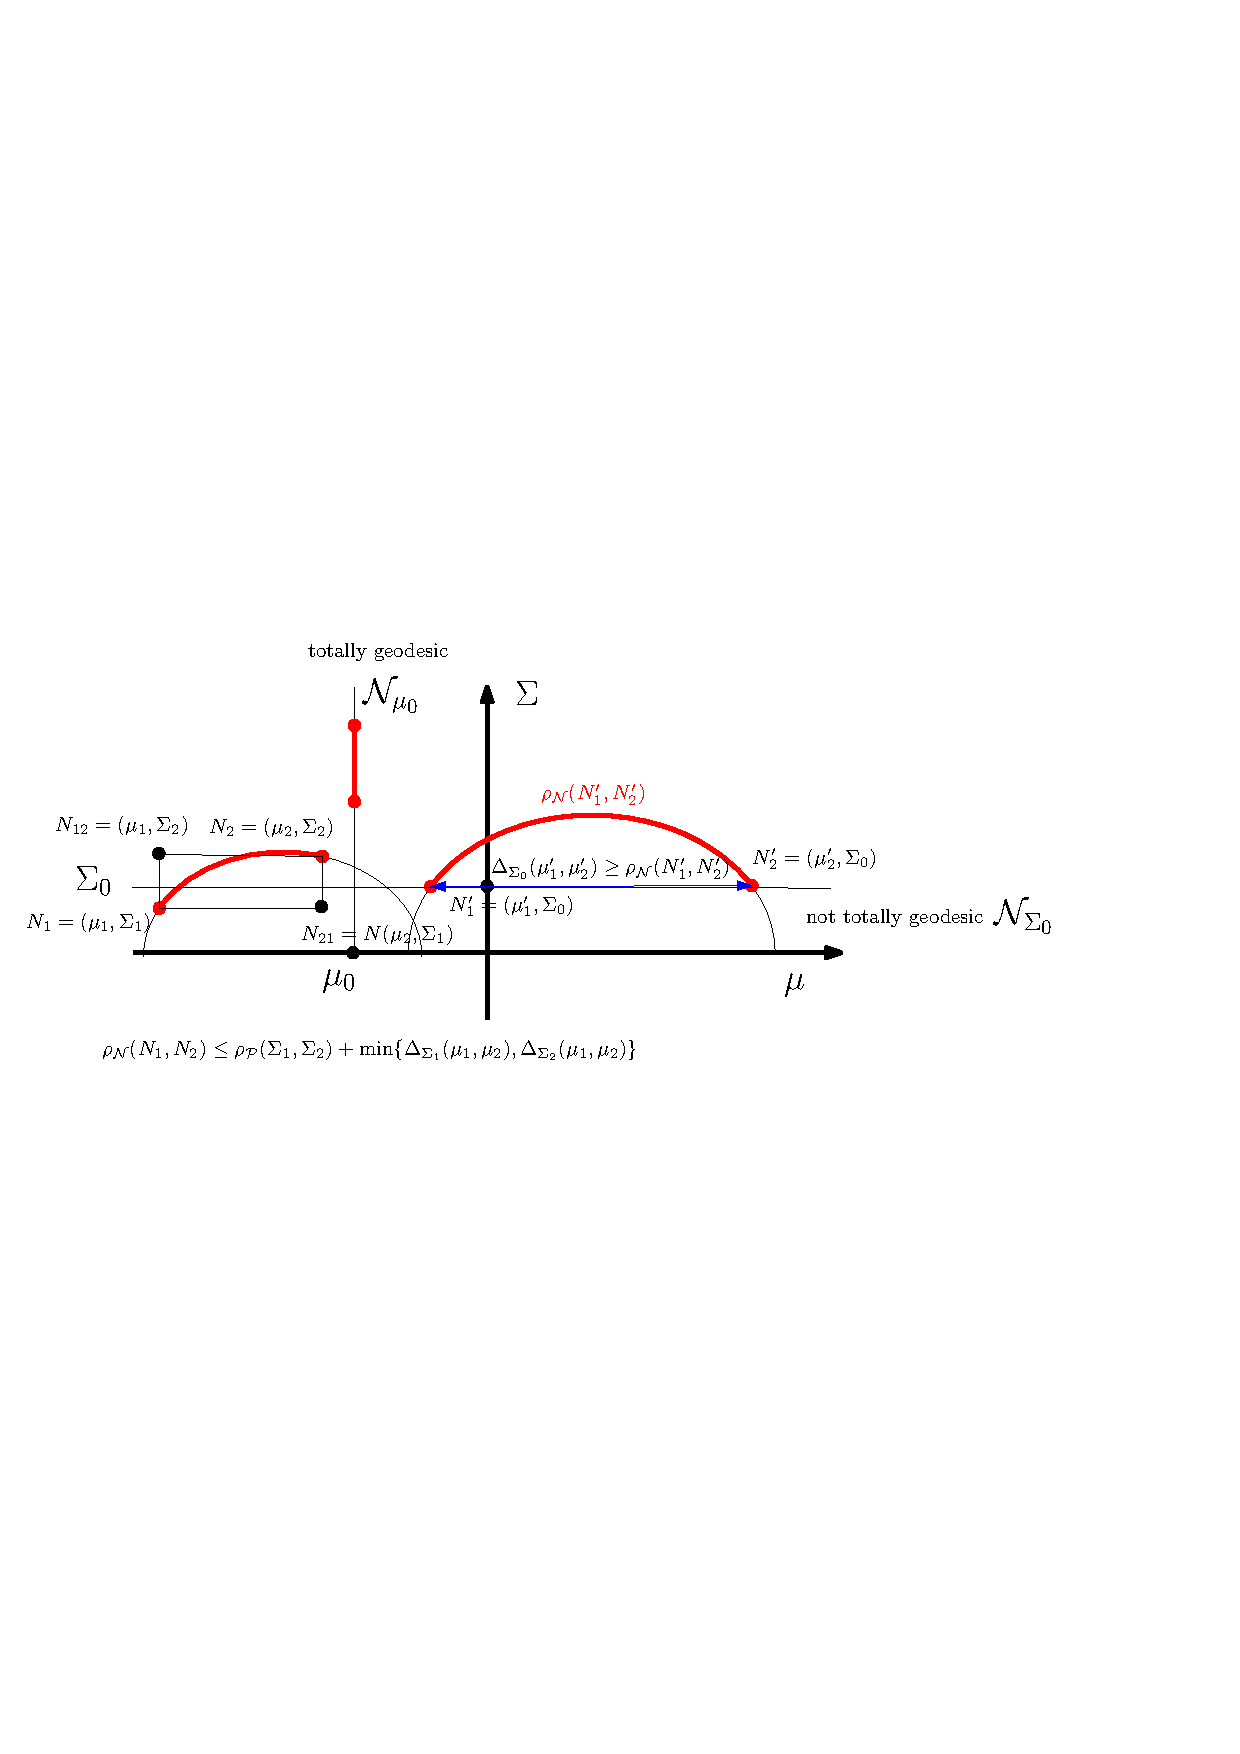
\includegraphics[width=0.8\textwidth]{FigIpe-MVNSubmanifoldUpperPlane.pdf}
%
\caption{
The submanifolds $\calN_{\Sigma}$ are not totally geodesic (i.e., $\rho_\calN(N_1',N_2')$ is upper bounded by their Mahalanobis distance) but the submanifolds $\calN_\mu$ are totally geodesic.
Using the triangle inequality of the Riemannian metric distance $\rho_\calN$, we can upper bound $\rho_\calN(N_1,N_2)$.
 \label{fig:totallynottotally}}
\end{figure}


In general, the~difficulty with calculating the Fisher--Rao distance comes from the fact~that 
\begin{enumerate}
\item  we do not know the Fisher–Rao geodesics with boundary value conditions (BVP) in closed form but the geodesics with initial value conditions~\cite{calvo1991explicit} (IVP) are known explicitly using the natural parameters $(\Sigma^{-1}\mu,\Sigma^{-1})$ of MVNs,
\item we must integrate the line element $\ds_\calN$ along the geodesic.
\end{enumerate}

As we shall see in {Section} %OK! MDPI: We added “Section” here, please confirm. the following highlights are the same
 \ref{sec:approxlength}, the~above first problem is much harder to solve than the second problem which can be easily approximated by discretizing the curve. 
The lack of a closed-form formula and fast and good approximations for $\rho_{\calN}$ between MVNs is a current limiting factor for its use in applications. 
Indeed, many applications (e.g., \cite{Sra-2016,nguyen2021geomnet}) consider the restricted case of the Rao distance between zero-centered MVNs which have closed form (distance of Equation~(\ref{eq:RaoCMVN}) in the SPD cone). 
The SPD cone is a symmetric Hadamard manifold, and its isometries have been fully studied and classified in~\cite{SPDisometries-2018} (\S{4}%Yes, correct. MDPI: Please check if it should be “Section 4”.
).
The Fisher–Rao geometry of zero-centered generalized MVNs was recently studied in~\cite{verdoolaege2012geometry}.



%%%
\subsection{Contributions and Paper~Outline}
%%%
The main contribution of this paper is to propose an approximation of $\rho_{\calN}$ based on Calvo and Oller's embedding~\cite{SDPMVN-1990}  (C\&O for short) and report its experimental performance.
First, we concisely recall C\&O's family of embeddings $f_\beta$ of $\calN(d)$ as submanifolds $\barN_\beta$ of $\calP(d+1)$ in Section~\ref{sec:CO}.
Next, we present our approximation technique in Section~\ref{sec:approxFR}  which differs from the usual geodesic shooting approach~\cite{MVNGeodesicShooting-2014}, and report experimental results.
Finally, we study some information–geometric properties~\cite{IG-2016} of the isometric embedding in {Section}~\ref{sec:prop} such as the fact that it preserves mixture geodesics (embedded C\&O submanifold is autoparallel with respect to the mixture affine connection) but not exponential geodesics.
Moreover, we prove that the Fisher–Rao distance between multivariate normal distributions sharing the same covariance matrix is a scalar function of their Mahalanobis distance in {Section}~\ref{sec:FRsamecovar} using the framework of Eaton~\cite{eaton1989group} of maximal invariants.

%%%
\subsection{A Closed-Form Formula for the Fisher–Rao Distance between Normal Distributions Sharing the Same Covariance Matrix}\label{sec:FRsamecovar}
%%%%

Consider the Fisher–Rao distance between $N_1=(\mu_1,\Sigma)$ and $N_1=(\mu_2,\Sigma)$ for a fixed covariance matrix $\Sigma$ and the translation action $a.\mu:=\mu+a$ of the translation group $\bbR^d$ (a subgroup of the affine group). Both the Fisher--Rao distance and the Mahalanobis distance are invariant under translations:
$$
\rho_\calN((\mu_1+a,\Sigma),(\mu_2+a,\Sigma))=\rho_\calN((\mu_1,\Sigma),(\mu_2,\Sigma)),\quad
\Delta_\Sigma(\mu_1+a,\mu_2+a)=\Delta_\Sigma(\mu_1,\mu_2).
$$
To prove that $\rho_\calN((\mu_1,\Sigma),(\mu_2,\Sigma))=h_\FR(\Delta_\Sigma(\mu_1,\mu_2))$ for a scalar function $h_\FR(\cdot)$, we shall prove that the Mahalanobis distance is a maximal invariant, and~use the framework of maximal invariants of Eaton~\cite{eaton1989group} (Chapter~2) who proved that any other invariant function is necessarily a function of a maximal invariant, i.e.,~a function of the Mahalanobis distance in our~case.

The Mahalanobis distance is a maximal invariant because  
we can write $\Delta_\Sigma(\mu_1,\mu_2)=\Delta_1(0,\Delta_\Sigma(\mu_1,\mu_2))$ and when
$\Delta_\Sigma(\mu_1,\mu_2)=\Delta_\Sigma(\mu_1',\mu_2')$ in 1D   there exists $a\in\bbR$ such that $(\mu_1+a,\mu_2+a)=(\mu_1',\mu_2')$.
We must prove equivalently that when $|m_1-m_2|=|m_1'-m_2'|$ that 
there exists $a\in\bbR$ such {that}  
 $(m_1+a,m_2+a)=(m_1',m_2')$. 
Assume without loss of generality that $m_1\geq m_2$.
When $m_1-m_2=m_1'-m_2'$, there exists  $a=m_1'-m_1$ so that  $m_1'=a.m_1=m_1+a$ and $m_2'=a.m_2=m_2+a$ with $m_1'-m_2'=m_1-m_2$.
Thus, using Eaton's theorem~\cite{eaton1989group}, there exists a scalar function $h_\FR$ such that 
$\rho_\calN((\mu_1,\Sigma),(\mu_2,\Sigma))=h_\FR(\Delta_\Sigma(\mu_1,\mu_2))$.


\textls[-35]{To find explicitly the scalar function $h_\FR(\cdot)$, let us consider the univariate case of normal distributions for which the Fisher–Rao distance is given in closed form in Equation~(\ref{eq:FR1D}). In~that case, the univariate Mahalanobis distance is $\Delta_{\sigma^2}(\mu_1,\mu_2)=\sqrt{(\mu_2-\mu_1)(\sigma^2)^{-1}(\mu_2-\mu_1)}=\frac{|\mu_2-\mu_1|}{\sigma}$ and we can write formula of Equation~(\ref{eq:FR1D}) as $h_\FR(\Delta_{\sigma^2}(\mu_1,\mu_2))$ with}
\begin{eqnarray}
h_\FR(u) &=& \sqrt{2}\,\log\left(\frac{\sqrt{8+u^2}+u}{\sqrt{8+u^2}-u}\right),\label{eq:h1d}\\
 &=& \sqrt{2}\,\arccosh\left(1+\frac{1}{4}u^2\right),\label{eq:h1dbis}
\end{eqnarray}
using the identities
$$
\log(x)=\arccosh\left(\frac{1+x^2}{2x}\right)=\arctanh\left(\frac{x^2-1}{1+x^2}\right), \quad x>1,
$$
where $\arctanh(u)=\frac{1}{2}\log\frac{1+u}{1-u}$.
 
\begin{Proposition}\label{prop:FRsamecovar}
The Fisher–Rao distance $\rho_\calN((\mu_1,\Sigma),(\mu_2,\Sigma))$ between two MVNs with same covariance matrix is
\begin{eqnarray}\label{eq:FRsamecovar}
\rho_\calN((\mu_1,\Sigma),(\mu_2,\Sigma)) &=&\rho_\calN((0,1),(\Delta_\Sigma(\mu_1,\mu_2),1)),\\
&=& \sqrt{2}\,\log\left(\frac{\sqrt{8+\Delta_\Sigma^2(\mu_1,\mu_2)}+\Delta_\Sigma(\mu_1,\mu_2)}{\sqrt{8+\Delta_\Sigma^2(\mu_1,\mu_2)}-\Delta_\Sigma(\mu_1,\mu_2)}\right),\\
&=& \sqrt{2}\, \arccosh\left(1+\frac{1}{4}\Delta_\Sigma^2(\mu_1,\mu_2)\right),\label{eq:FRh1dbis}
\end{eqnarray}
where $\Delta_\Sigma(\mu_1,\mu_2)=\sqrt{(\mu_2-\mu_1)^\top\Sigma^{-1}(\mu_2-\mu_1)}$ is the Mahalanobis distance.
\end{Proposition}

Indeed, notice that the $d$-variate Mahalanobis distance $\Delta_\Sigma(\mu_1,\mu_2)$ can be interpreted as a univariate Mahalanobis distance between the standard normal distribution $N(0,1)$ and $N(\Delta_\Sigma(\mu_1,\mu_2),1)$:
$$
\Delta_\Sigma(\mu_1,\mu_2)=\Delta_1(0,\Delta_\Sigma(\mu_1,\mu_2)).
$$
Thus, we have $\rho_\calN((\mu_1,\Sigma),(\mu_2,\Sigma))=\rho_\calN((0,1),(\Delta_\Sigma(\mu_1,\mu_2),1))$,
where the right-hand-side term is the univariate Fisher–Rao distance of Equation~(\ref{eq:FR1D}).
Let us notice that the square length element on $\calM_\Sigma$ is $\ds^2=\dmu^\top\Sigma^{-1}\dmu=\Delta_\Sigma^2(\mu,\mu+\dmu)$.
This result can be extended to elliptical distributions~\cite{chen2021upper} ({Theorem~1}% Yes, it is thm 1 of Ref. 12 MDPI: There is no Theorem 1 in the text. Please confirm if this Theorem belongs to Ref.12.
).

Let us corroborate this result by checking the formula of Equation~(\ref{prop:FRsamecovar}) with two examples in the literature:
In~\cite{strapasson2015bounds} {(Figure 4)}%Yes, fig 4 is of Ref. 38 MDPI: Please check if Figure 4 belongs to Ref.38, if not, please cite the figure in the text and ensure the first citation of each figure appears in numerical order. so Figure 4 should be cited after the Figure 3. the following highlights are the same
, we Fisher–Rao distance between
$N_1=(0,I)$ and $N_2=\left(\vectortwo{\frac{1}{2}}{\frac{1}{2}},I\right)$ is studied.
We find $\rho_\calN(N_1,N_2)=0.69994085$ in accordance with their result shown in {Figure~4}.
The second example is Example~1 of~\cite{FRMVNReview-2020} (p. 11) with
$N_1=\left(\vectortwo{-1}{0},\Sigma\right)$ and $N_2=\left(\vectortwo{6}{3},\Sigma\right)$ for 
$\Sigma=\mattwotwo{1.1}{0.9}{0.9}{1.1}$.
Formula of Equation~(\ref{eq:FRsamecovar}) yields the Fisher–Rao distance $5.006483034546878$
in accordance with~\cite{FRMVNReview-2020} which reports $5.00648$.

Similarly, the~statistical Ali–Silvey–Csisz\'ar $f$-divergences~\cite{fdiv-AliSilvey-1966,Csiszar-1967}
$$
I_f[p_{(\mu_1,\Sigma)}:p_{(\mu_2,\Sigma)}]=\int_{\bbR^d}  p_{(\mu_1,\Sigma)}(x)\, f\left(\frac{ p_{(\mu_2,\Sigma)}}{ p_{(\mu_1,\Sigma)}}\right)  \mathrm{d}x,
$$
between two MVNs sharing the same covariance matrix are increasing functions of the Mahalanobis distance because the $f$-divergences between two MVNs sharing the same covariance matrix are invariant under the action of the translation group~\cite{nielsen2022note}. Thus, we have 
$I_f[p_{(\mu_1,\Sigma}:p_{(\mu_2,\Sigma)}]=h_f(\Delta_\Sigma(\mu_1,\mu_2))$. 
Since $\Delta_\Sigma(\mu_1,\mu_2)=\Delta_1(0,\Delta_\Sigma(\mu_1,\mu_2))$, we thus have
$$
I_f[p_{(\mu_1,\Sigma}:p_{(\mu_2,\Sigma)}]=h_f(\Delta_1(0,\Delta_\Sigma(\mu_1,\mu_2))=I_f[p_{(0,1}:p_{(\Delta_\Sigma(\mu_1,\mu_2),1)}],
$$
where the right-hand side $f$-divergence is between univariate normal distributions.
See Table~2 of~\cite{nielsen2022note} for some explicit functions $h_f$.

%We can further consider the subfamily 
%$$
%\calN_{[\Sigma]}=\left\{(\mu,\alpha\Sigma) \st \mu\in\bbR^d, \alpha\in\bbR_{>0}\right\},
%$$
 %of normal distributions with covariance matrices being any $\alpha\Sigma$ for some prescribed matrix $\Sigma$ but varying $\alpha>0$.
%Then we consider the group of translation-scale $\bbR^d\times\bbR_{>0}$ and prove similarly that the scale Mahalanobis distance
%$$
%\Delta_\Sigma(\mu_1,\alpha_1;\alpha_2,\alpha_2):=\frac{1}{\alpha_1\alpha_2}\Delta_\Sigma(\mu_1,\mu_2)
%$$ 
%is a maximal invariant. It follows that the Fisher--Rao distance is a function of $\Delta_\Sigma(\mu_1,\alpha_1;\alpha_2,\alpha_2)$ which can be found by inspecting the closed-form formula of the 1D Fisher--Rao distance.
%Thus we get
%$$
%\rho_\calN(N(\mu_1,\alpha_1\Sigma),N(\mu_1,\alpha_1\Sigma))=\sqrt{2}\, \arccosh\left(1+\frac{1}{4\alpha_1\alpha_2}\Delta_\Sigma^2(\mu_1,\mu_2)\right).
%$$
%%% Using affine invariance with $A=\frac{1}{\alpha_1}L^{-1}$, we get case N(0,I) N(\frac{1}{\sqrt{\alpha_1}L^{-1}(\mu_2-\mu_1),\frac{\alpha_2}{\alpha_1}I)


%%
\section{Calvo and Oller's Family of Diffeomorphic~Embeddings}\label{sec:CO}
%%
Calvo and Oller~\cite{SDPMVN-1990,SDPElliptical-2002} noticed that we can  embed the space of normal distributions in $\calP(d+1)$ by  using the following   mapping:
\begin{equation}
f_{\beta}(N)=f_{\beta}(\mu,\Sigma)=
  \mattwotwo{\Sigma+\beta\mu\mu^\top}{\beta\mu}{\beta\mu^\top}{\beta}\in\calP(d+1),
\end{equation}
where $\beta\in\bbR_{>0}$ and $N=N(\mu,\Sigma)$.
Notice that since the dimension of $\calP(d+1)$ is $\frac{(d+1)(d+2)}{2}$, we only use $\frac{(d+1)(d+2)}{2}-\frac{d(d+3)}{2}=1$ extra dimension for embedding $\calN(d)$ into $\calP(d+1)$. 
By foliating $\bbP=\bbR_{>0}\times \bbP_c$ where $\bbP_c=\{P\in\bbP\st |P|=c\}$ denotes the subsets of $\bbP$ with determinant $c$, we obtain the following Riemannian Calvo and Oller metric on the SPD cone:
\begin{eqnarray*}
\ds^2_\CO &=& \frac{1}{2}\tr\left(\left(f^{-1}(\mu,\Sigma)\mathrm{d}f(\mu,\Sigma)\right)^2\right),\\
&=& \frac{1}{2}\left(\frac{\dbeta}{\beta}\right)^2 + \beta\dmu^\top \Sigma^{-1}\dmu+\frac{1}{2}\tr\left(\left(\Sigma^{-1}\dSigma\right)^2\right).
\end{eqnarray*}


Let 
$$
\barN_\beta(d) = \left\{\barP=f_{\beta}(\mu,\Sigma) \st (\mu,\Sigma)\in \calN(d)=\bbR^d\times\calP(d)\right\}
$$
 denote the submanifold of $\calP(d+1)$ of codimension $1$, and~$\barN=\barN_1$ (i.e., $\beta=1$). 
The family of mappings $f_{\beta}$ provides diffeomorphisms between $\calN(d)$ and $\barN_\beta(d)$. 
Let $f_{\beta}^{-1}(\barP)=(\mu_\barP,\Sigma_\barP)$ denote the inverse mapping for $\barP\in\barN_\beta(d)$, and~let $f=f_1$ (i.e., $\beta=1$): 
$$
f(N)=f(\mu,\Sigma)=\mattwotwo{\Sigma+\mu\mu^\top}{\mu}{\mu^\top}{1}.
$$

By equipping the cone $\calP(d+1)$ by the trace metric~\cite{moakher2011riemannian,EllipticIsometrySPD-2021} (also called the affine invariant Riemannian metric, AIRM) scaled by $\frac{1}{2}$: 
$$
g_P^\trace(P_1,P_2):=\tr(P^{-1}P_1P^{-1}P_2)
$$ 
 (yielding the squared line element $\ds_\calP^2=\frac{1}{2}\tr((P\,\dP)^2)$),
Calvo and Oller~\cite{SDPMVN-1990} proved that $\barN(d)$ is isometric to $\calN(d)$ (i.e., the~Riemannian metric of $\calP(d+1)$ restricted to $\calN(d)$ coincides with the Riemannian metric of $\calN(d)$ induced by $f$) but $\barN(d)$ is not totally geodesic (i.e., the~geodesics $\gamma_\calP(\barP_1,\barP_2;t)$ for $\barP_1=f(N_1),\barP_2=f(N_2)\in\barN(d)$ leaves the embedded normal submanifold $\barN(d))$.
Please note that $g_P^\trace$ can be interpreted as the Fisher metric for the family $\calN_0$ of $0$-centered normal distributions.
Thus, we have $(\calN(d),g^\Fisher)\hookrightarrow (\calP(d+1),g^\trace)$, and~the following diagram between parameter spaces and corresponding distributions:
$$
\begin{array}{ccc}
\calN(d) & \hookrightarrow  &\calN_0(d+1)\\
\updownarrow & & \updownarrow\\
\Lambda(d) & \hookrightarrow & \bbP(d+1)
\end{array}
$$



\begin{Remark}
The trace metric was first studied by Siegel~\cite{siegel2014symplectic,nielsen2020siegel} using the wider scope of complex symmetric matrices with positive–definite imaginary parts generalizing the Poincar\'e upper half-plane (see Appendix~\ref{sec:Siegel}).
\end{Remark}



We omit to specify the dimensions and write for short $\calN$, $\barN$, and $\calP$  when clear from the context.
Thus, C\&O proposed to use the embedding $f=f_{1}$ to give a lower bound $\rho_\CO$ of the Fisher–Rao distance $\rho_\calN$ between normals:
\begin{equation}
\mathrm{LC}_\CO:\quad \rho_{\calN}(N_1,N_2)\geq \rho_{\CO}(\underbrace{f(\mu_1,\Sigma_1)}_{\barP_1},\underbrace{f(\mu_2,\Sigma_2)}_{\barP_2})=
\sqrt{\frac{1}{2}\sum_{i=1}^{d+1} \log^2 \lambda_i(\barP_1^{-1}\barP_2)}.
\end{equation}

We let $\rho_{\CO}(N_1,N_2)=\rho_\CO(f(N_1),f(N_2))$.
The $\rho_\CO$ distance is invariant under affine transformations such as the Fisher–Rao distance of Property~\ref{prop:aifr}:


\begin{Property}[affine invariance of C\&O distance~\cite{SDPMVN-1990}]\label{prop:aico}
For all $A\in\GL(d), a\in\bbR^d$,
we have
$\rho_{\CO}((A\mu_1+a,A\Sigma_1 A^\top),(A\mu_2+a,A\Sigma_2 A^\top)) = \rho_{\CO}(N(\mu_1,\Sigma_1),N(\mu_2,\Sigma_2))$.
\end{Property}

When $\Sigma_1=\Sigma_2=\Sigma$, we have $|\barP_1|=|\barP_2|=|\Sigma|$.
Since the Riemannian geodesics $\gamma_\bbP(P_1,P_2;t)$ in the SPD cone are given by $\gamma_\bbP(P_1,P_2;t)=P_1^{\frac{1}{2}}(P_1^{-\frac{1}{2}}P_2P_1^{-\frac{1}{2}})^t P_1^{\frac{1}{2}}$~\cite{RieMinimax-2013} (also written $\gamma_\SPD(P_1,P_2;t)$), we have
$|\gamma_\bbP(P_1,P_2;t)|=|\Sigma|$. 
Although the submanifold $\bbP_c=\{P\in\bbP\st |P|=c\}$ is totally geodesic with respect to the trace metric, it is not totally geodesic with respect to $\frac{1}{2}\tr((\barP\mathrm{d}\barP)^2)$.
Thus, although $\gamma_\bbP(P_1,P_2)\in\barN$, it does not correspond to the embedded MVN geodesics with respect to the Fisher metric.
The C\&O distance between two MVNs $N(\mu_1,\Sigma)$ and $N(\mu_2,\Sigma)$ sharing the same covariance matrix~\cite{SDPMVN-1990} is
\begin{equation}\label{eq:cosamecovar}
\rho_{\CO}(N(\mu_1,\Sigma),N(\mu_2,\Sigma))=\arccosh\left(1+\frac{1}{2}\Delta_\Sigma^2(\mu_1,\mu_2)\right),
\end{equation}
where $\arccosh(x):=\log(x+\sqrt{x^2-1})$ for $x\geq 1$ and $\Delta_\Sigma(\mu_1,\mu_2)$ is the Mahalanobis distance between $N(\mu_1,\Sigma)$ and $N(\mu_2,\Sigma)$. In~that case,  we thus have $\rho_{\CO}(N(\mu_1,\Sigma),N(\mu_2,\Sigma))=h_\CO(\Delta_\Sigma(\mu_1,\mu_2))$ where
$h_\CO(u)=\arccosh\left(1+\frac{1}{2}u^2\right)$ is a strictly monotone increasing function.
Let us note in passing that in~\cite{SDPMVN-1990} (Corollary, page 230) there is a confusing or typographic error since the distance is reported as $\arccosh\left(1+\frac{1}{2}d_M(\mu_1,\mu_2)\right)$ where $d_M$ denotes ``Mahalanobis distance''~\cite{mahalanobis1936generalised}. Therefore, either $d_M=\Delta_\Sigma^2$, Mahalanobis $D^2$-distance, or~there is a missing square in the equation of the Corollary page 230.
To obtain a flavor of how good is the approximation of the C\&O distance, we may consider the same covariance case where we have both closed-form solutions for $\rho_{\calN}$ (Equation~(\ref{eq:FRh1dbis})) and $\rho_{\CO}$ (Equation~(\ref{eq:cosamecovar})).
Figure~\ref{fig:qualityFRCO} plots the two functions $h_\CO$ and $h_\FR$ (with $h_\CO(u)\leq h_\FR(u)\leq u$ for $u\in[0,\infty)$).

\begin{figure}[H]

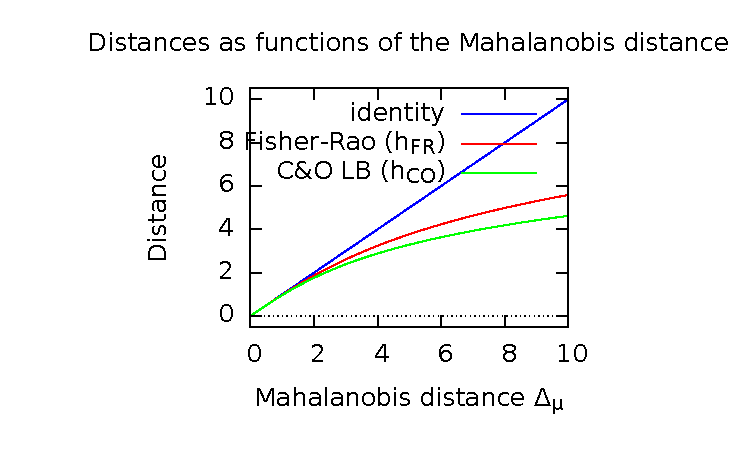
\includegraphics[width=0.75\textwidth]{Plot-FRCOLB.pdf}
\caption{Quality of the C\&O lower bound compared to the exact Fisher–Rao distance in the case of $N_1,N_2\in\calM_\Sigma$ (MVNs sharing the same covariance matrix $\Sigma$). We have $\rho_\CO\leq \rho_\calN\leq \Delta_\Sigma$. \label{fig:qualityFRCO}}
\end{figure}


Let us  remark that similarly all $f$-divergences between $N_1=(\mu_1,\Sigma)$ and $N_2=(\mu_2,\Sigma)$ are scalar functions of their Mahalanobis distance $\Delta_\Sigma(\mu_1,\mu_2)$ too, see~\cite{nielsen2022note}.


The C\&O distance $\rho_{\CO}$ is a metric distance that has been used in many applications ranging from computer vision~\cite{ceolin2012computing,wang2017g2denet,nguyen2021geomnet,miyamoto2022fisher} to signal/sensor processing, statistics~\cite{kurtek2015bayesian,marti2016optimal}, machine learning~\cite{tang2018information,DA-FisherRaoMVN-2015,li2016local,liang2019fisher,picot2022adversarial,collas2022use} and analogical reasoning~\cite{murena2018opening}.

\begin{Remark}\label{rk:secondco}
In a second paper, Calvo and Oller~\cite{SDPElliptical-2002} noticed that we can embed normal distributions in $\calP(d+1)$ by the following more general mapping ({Lemma 3.1}%Yes, of Ref. 32 MDPI: Please confirm that Lemma 3.1 belongs to Ref.32.
~\cite{SDPElliptical-2002}):
\begin{equation}
g_{\alpha,\beta,\gamma}(\mu,\Sigma)=
|\Sigma|^{\alpha} \mattwotwo{\Sigma+\beta\gamma^2\mu\mu^\top}{\beta\gamma\mu}{\beta\gamma\mu^\top}{\beta}\in\calP(d+1),
\end{equation}
where $\alpha\in\bbR$, $\beta\in\bbR_{>0}$ and $\gamma\in\bbR$.
It is show in~\cite{SDPElliptical-2002} that the induced length element is
\begin{eqnarray*}
\ds^2_{\alpha,\beta,\gamma}&=&\frac{1}{2}\left(
\alpha ((d+1)+2\alpha)\tr^2(\Sigma^{-1}\dSigma)+\tr((\Sigma^{-1}\dSigma)^2)\right.\\
&&\left.
+2\beta\gamma^2\dmu^\top\Sigma^{-1}\dmu+2\alpha \tr(\Sigma^{-1}\dSigma)\frac{\dbeta}{\beta}+
\left(\frac{\dbeta}{\beta}\right)^2
\right).
\end{eqnarray*}
When $\gamma=\beta=1$, we have
$$
\ds^2_\alpha=\frac{1}{2}\left(
\alpha ((d+1)+2\alpha)\tr^2(\Sigma^{-1}\dSigma)+\tr((\Sigma^{-1}\dSigma)^2)
+2\beta\gamma^2\dmu^\top\Sigma^{-1}\dmu
\right).
$$
Thus, to cancel the term $\tr^2(\Sigma^{-1}\dSigma)$, we may either choose $\alpha=0$ or $\alpha=-\frac{2}{1+d}$.

In some applications~\cite{popovic2022measure}, the~embedding
\begin{equation}\label{eq:g}
g_{-\frac{1}{d+1},1,1}(\mu,\Sigma)=|\Sigma|^{-\frac{1}{d+1}} \mattwotwo{\Sigma+\mu\mu^\top}{\mu}{\mu^\top}{1}:=\hat{f}(\mu,\Sigma),
\end{equation}
is used to ensure that $\left|g_{-\frac{1}{d+1},1,1}(\mu,\Sigma)\right|=1$.
That is normal distributions are embedded diffeomorphically into the submanifold of positive–definite matrices with a unit determinant (also called SSPD, acronym of Special SPD).
In~\cite{SDPElliptical-2002}, C\&O showed that there exists a second isometric embedding of the Fisher–Rao Gaussian manifold $\calN(d)$ into a submanifold of the cone $\calP(d+1)$: $f_\SSPD(\mu,\Sigma)=|\Sigma|^{-\frac{2}{d+1}} \mattwotwo{\Sigma+\mu\mu^\top}{\mu}{\mu^\top}{1}$.
Let $\hat{P}=f_\SSPD(\mu,\Sigma)$. This  mapping can be understood as taking the elliptic isometry ${P}\mapsto {|P|}^{-\frac{2}{d+1}} {P}$ of $P\in\calP(d+1)$~\cite{EllipticIsometrySPD-2021} since $|\Sigma|=|\bar{P}(\mu,\Sigma)|$ (see proof in Proposition~\ref{prop:KL}). 
It follows that
$$
\rho_\CO(N_1,N_2)=\rho_\calP(\barP_1,\barP_2)=\rho_\calP(\hat{P}_1,\hat{P}_2) \leq \rho_\calN(N_1,N_2).
$$
Similarly, we could have mapped ${P}\mapsto P^{-1}$ to obtain another isometric embedding.
See the four types of elliptic isometric of the SPD cone described in~\cite{EllipticIsometrySPD-2021}.
Finally, let us remark that the SSPD submanifold is totally geodesic with respect to the trace metric but not with respect to the C\&O metric.
\end{Remark}


Interestingly, Calvo and Oller~\cite{calvo1991explicit} (p. 131) proved that $((\bar\mu_1,\ldots,\bar\mu_d),\diag(\bar\sigma_1^2,\ldots,\bar\sigma_d^2))$
 is a maximal invariant for the action of the affine group $\Aff(d)$, where $\bar\mu=Q^{-1}(\mu_2-\mu_1)$ and 
$\Sigma_2\Sigma_1^{-1}=Q\,\diag(\bar\sigma_1^2,\ldots,\bar\sigma_d^2)\, Q^{-1}$ (in~\cite{calvo1991explicit}, the~authors considered 
$\Sigma_1\Sigma_1^{-2}$).
Thus, we consider the following dissimilarity
\begin{equation}\label{eq:DCO}
D_\CO(N(\mu_1,\Sigma_1),N(\mu_2,\Sigma_2))=\sqrt{2}\, \sqrt{\sum_{i=1}^d \log^2\left(\frac{1+\Delta(0,1;\bar\mu_i,\bar\sigma_i)}{1-\Delta(0,1;\bar\mu_i,\bar\sigma_i)} \right)}.
\end{equation}
Dissimilarity $D_\CO$ is symmetric (i.e., $D_\CO(N_1,N_2)=D_\CO(N_2,N_1)$) and $D_\CO(N_1,N_2)=0$ if and only if $N_1=N_2$.
Please note that when $d=1$, $D_\CO$ is different from the Fisher--Rao distance of Equation~(\ref{eq:FR1D}).
%We found experimentally that $D_\CO$ is smaller or equal than $\rho_\CO$ which is a lower bound on the Fisher--Rao distance $\rho_\calN$.
%As mentioned in~\cite{calvo1991explicit} (p. 133), ``the question whether [$D_\CO$] satisfies the triangle inequality remains open.''


%%%
\section{Approximating the Fisher--Rao~Distance}\label{sec:approxFR}
%%%

\subsection{Approximating Length of~Curves}\label{sec:approxlength}

Recall that the Fisher--Rao's distance~\cite{micchelli2005rao} is the Riemannian geodesic distance
$$
\rho_\calN(N(\lambda_1),N(\lambda_2))=\inf_{\substack{c(t)\\ c(0)=p_{\lambda_1}\\ c(1)=p_{\lambda_2}}}  \, \left\{\Length(c)\right\},
$$
\noindent where 
$$
\Length(c)=\int_0^1 \underbrace{\sqrt{\inner{\dot c(t)}{\dot c(t)}}_{c(t)}}_{\ds_\calN(t)} \dt.
$$



We can approximate the Rao distance $\rho_\calN(N_1,N_2)$ by discretizing regularly  any smooth curve $c(t)$ joining 
$N_1=c(0)$ to $N_2=c(1)$ (Figure~\ref{fig:method}):
$$
\rho_\calN(N_1,N_2)\leq \frac{1}{T} \sum_{i=1}^{T-1} \rho_\calN\left(c\left(\frac{i}{T}\right),c\left(\frac{i+1}{T}\right)\right),$$
with equality holding iff $c(t)=\gamma_\calN(N_1,N_2;t)$ is the Riemannian geodesic defined by the Levi–Civita metric connection induced by the Fisher information~metric.

When the number of discretization steps $T$ is sufficiently large, the~normal distributions 
$c\left(\frac{i}{T}\right)$ and $c\left(\frac{i+1}{T}\right)$ are close to each other, and~we can approximate 
$\rho_\calN\left(c\left(\frac{i}{T}\right),c\left(\frac{i+1}{T}\right)\right)$ 
by $\sqrt{D_J\left[c\left(\frac{i}{T}\right),c\left(\frac{i+1}{T}\right)\right]}$, where $D_J[N_1,N_2]=D_\KL[N_1,N_2]+D_\KL[N_2,N_1]$ is Jeffreys divergence, and~$D_\KL$ is the Kullback–Leibler divergence:
$$
D_\KL[p_{(\mu_1,\Sigma_1)}:p_{(\mu_2,\Sigma_2)}]
=\frac{1}{2}\left(
\tr(\Sigma_2^{-1}\Sigma_1)+\Delta\mu^\top\Sigma_2^{-1}\Delta\mu-d+\log\frac{|\Sigma_2|}{|\Sigma_1|}
\right).
$$
Thus, the costly determinant computations cancel each other in Jeffreys divergence (i.e., $\log\frac{|\Sigma_2|}{|\Sigma_1|}+\log\frac{|\Sigma_1|}{|\Sigma_2|}=0$) and we have:
$$
D_J[p_{(\mu_1,\Sigma_1)}:p_{(\mu_2,\Sigma_2)}]=\tr\left(\frac{\Sigma_2^{-1}\Sigma_1+\Sigma_1^{-1}\Sigma_2}{2}-I\right)
+\Delta\mu^\top\frac{\Sigma_1^{-1}+\Sigma_2^{-1}}{2}\Delta\mu.
$$
Figure~\ref{fig:method} summarizes our method to approximate the Fisher–Rao geodesic~distance.

\begin{figure}[H]

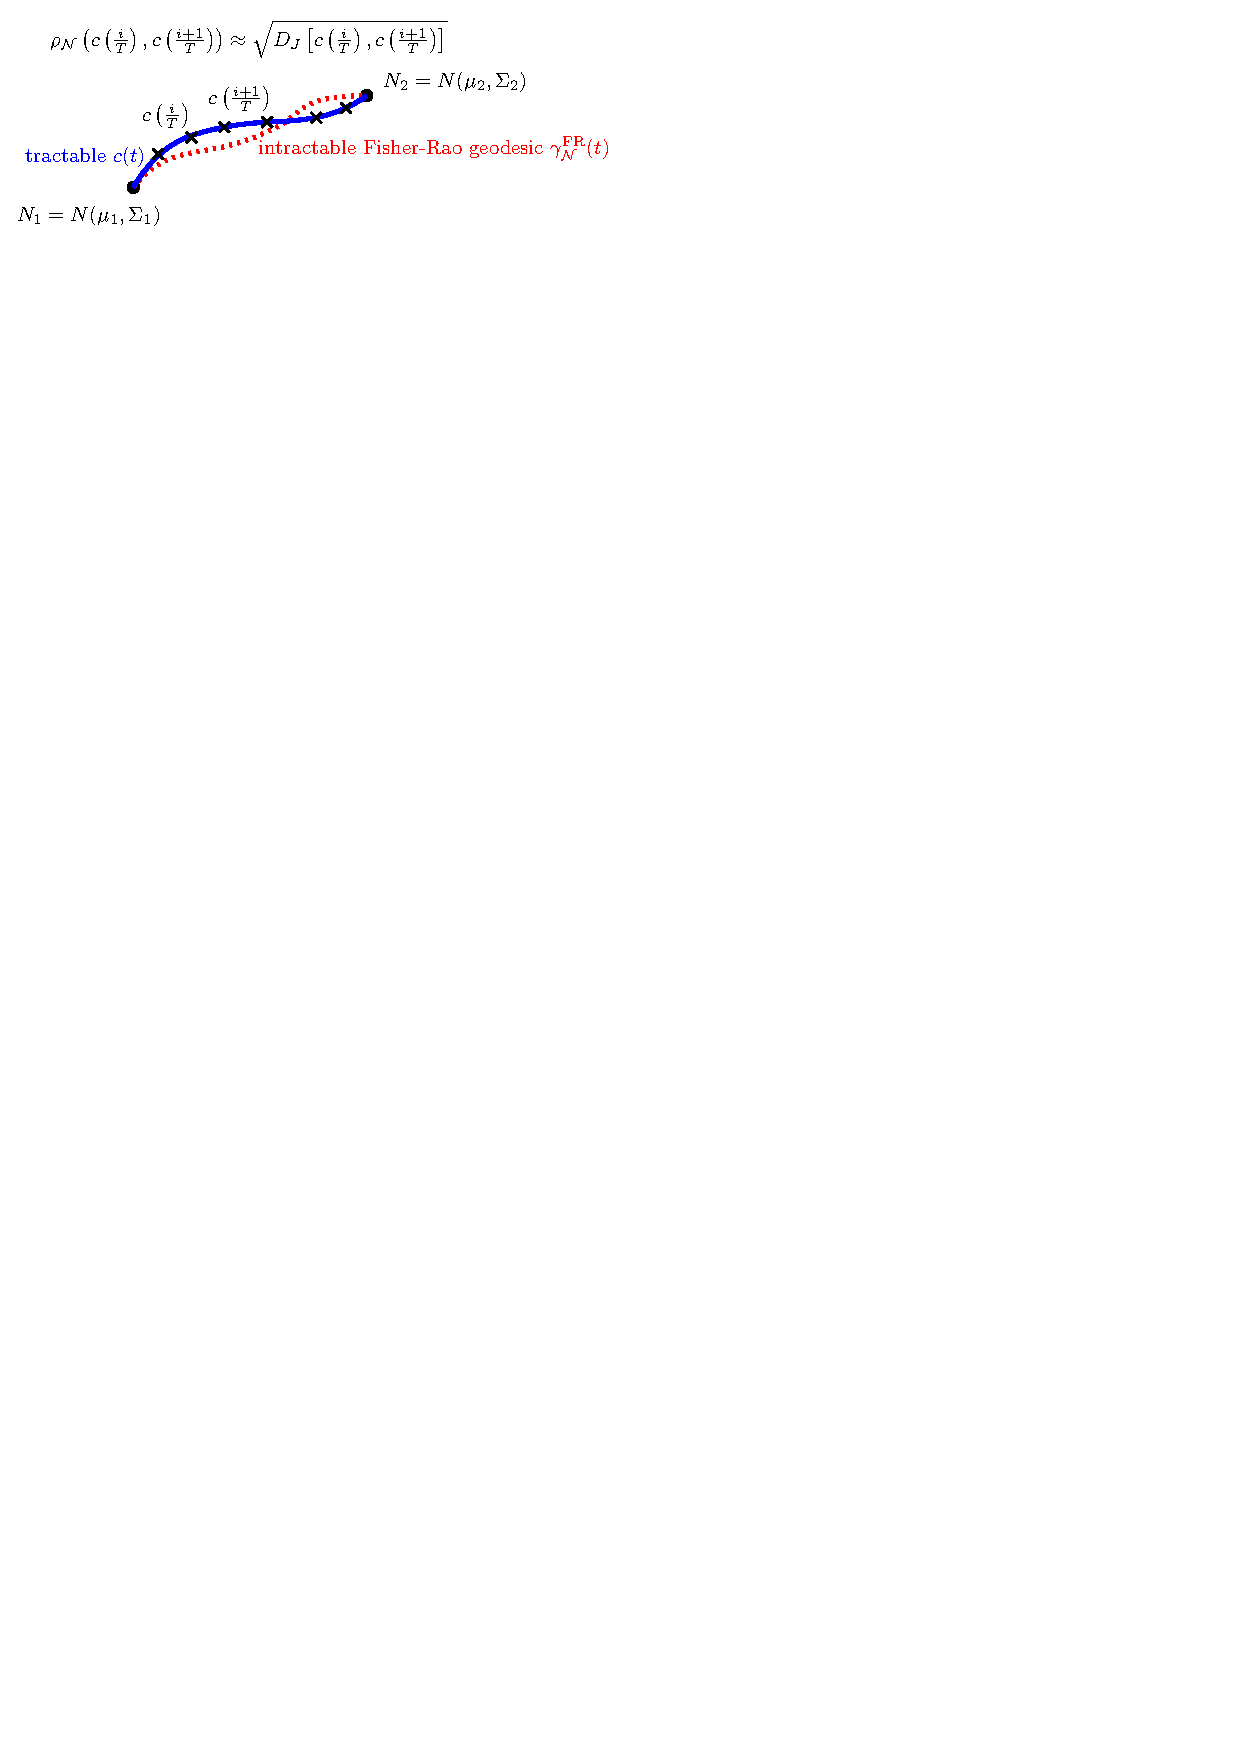
\includegraphics[width=0.8\textwidth]{FigIpe-ApproximationTractableCurve.pdf}
%
\caption{Approximating the Fisher–Rao geodesic distance $\rho_\calN(N_1,N_2)$: 
The Fisher–Rao geodesic $\gamma_\calN^{\mathrm{FR}}$ is not known in closed form.
 We consider a tractable curve $c(t)$, discretize $c(t)$ at $T+1$ points $c(\frac{i}{T})$ with $c(0)=N_1$ and $c(1)=N_2$, and~approximate $\rho_\calN\left(c\left(\frac{i}{T}\right),c\left(\frac{i+1}{T}\right)\right)$ by $\sqrt{D_J\left[c\left(\frac{i}{T}\right),c\left(\frac{i+1}{T}\right)\right]}$, considering that different tractable curves $c(t)$ yield different approximations.
 \label{fig:method}}
\end{figure}



In general, it holds that 
$$
I_f[p:q]\approx \frac{f''(1)}{2}\ds^2_\Fisher,
$$ 
between infinitesimally close distributions $p$ and $q$ ($\ds\approx \sqrt{\frac{2\,I_f[p:q]}{f''(1)}}$), where $I_f[\cdot:\cdot]$ denotes a $f$-divergence~\cite{IG-2016}.
The Jeffreys divergence is a $f$-divergence obtained for $f_J(u)=-\log u+u\log u$ with $f_J''(1)=2$.
It is thus interesting to find low computational cost $f$-divergences between multivariate normal distributions to approximate the infinitesimal length element $\ds$. 
Please note that $f$-divergences between MVNs are also invariant under the action of the affine group~\cite{nielsen2022note}.
Thus, for infinitesimally close distributions $p$ and $q$, this informally explains that $\ds_\Fisher$ is invariant under the action of the affine group (see Proposition~\ref{prop:aifr}).


 
Although the definite integral of the length element along the Fisher–Rao geodesic $\gamma_\calN^{\mathrm{FR}}$ is not known in closed form (i.e., Fisher–Rao distance), the~integral of the squared length element along the mixture geodesic $\gamma_\calN^m(N_1,N_2)$ 
and exponential geodesic $\gamma_\calN^e(N_1,N_2)$ coincide with Jeffreys divergence $D_J[N_1,N_2]$ between $N_1$ and $N_2$~\cite{IG-2016}:

\begin{Property}[\cite{IG-2016}]\label{prop:geolengthJeffreys}
We have $$
D_J[p_{\lambda_1},p_{\lambda_2}]=\int_0^1 \ds_\calN^2(\gamma^m_\calN(p_{\lambda_1},p_{\lambda_2};t))\dt =
\int_0^1 \ds_\calN^2(\gamma^e_\calN(p_{\lambda_1},p_{\lambda_2};t))\dt.
$$
\end{Property}

\begin{proof}
Let us report a proof of this remarkable fact in the general setting of Bregman manifolds.
Indeed, since 
$$
D_J[p_{\lambda_1},p_{\lambda_2}]=D_\KL[p_{\lambda_1}:p_{\lambda_2}]+D_\KL[p_{\lambda_2}:p_{\lambda_1}],
$$
and $D_\KL[p_{\lambda_1}:p_{\lambda_2}]=B_F(\theta(\lambda_2):\theta(\lambda_1))$, where $B_F$ denotes the Bregman divergence induced by the cumulant function of the multivariate normals and $\theta(\lambda)$ is the natural parameter corresponding to $\lambda$, we have
\begin{eqnarray*}
D_J[p_{\lambda_1},p_{\lambda_2}]&=&B_F(\theta_1:\theta_2)+B_F(\theta_2:\theta_1),\\
&=& S_F(\theta_1;\theta_2)=(\theta_2-\theta_1)^\top (\eta_2-\eta_1)=S_{F^*}(\eta_1;\eta_2),
\end{eqnarray*}
where $\eta=\nabla F(\theta)$ and $\theta=\nabla F^*(\eta)$ denote the dual parameterizations obtained by the Legendre–Fenchel convex conjugate  $F^*(\eta)$ of $F(\theta)$. Moreover, we have $F^*(\eta)=-h(p_{\mu,\Sigma})$~\cite{IG-2016}, i.e.,~the convex conjugate function is Shannon~negentropy.

Then we conclude using the fact that $S_F(\theta_1;\theta_2)=\int_0^1 \ds^2(\gamma(t))\dt=\int_0^1 \ds^2(\gamma^*(t))\dt$, 
i.e., the~symmetrized Bregman divergence amounts to integral energies on dual geodesics on a Bregman manifold.
The proof of this general property is reported in Appendix~\ref{sec:proof}.
\end{proof}
 
 

It follows the following upper bound on the Fisher--Rao distance:

\begin{Property}[Fisher--Rao upper bound]\label{prop:UBJ}
The Fisher–Rao distance between normal distributions is upper bounded by the square root of the Jeffreys divergence: $\rho_\calN(N_1,N_2) \leq\sqrt{D_J(N_1,N_2)}$.
\end{Property}

\begin{proof}
Consider the Cauchy–Schwarz inequality for positive functions $f(t)$ and $g(t)$:
 $\int_0^1 f(t)g(t)\dt\leq\sqrt{(\int_0^1 f(t)^2\dt)(\int_0^1 g(t)^2\dt)}$), and~let $f(t)=\ds_\calN(\gamma^c_\calN(p_{\lambda_1},p_{\lambda_2};t)$ and $g(t)=1$. 
Then we obtain: 
$$
\left(\int_0^1 \ds_\calN(\gamma^c_\calN(p_{\lambda_1},p_{\lambda_2};t)\dt\right)^2
\leq \left(\int_0^1 \ds_\calN^2(\gamma^c_\calN(p_{\lambda_1},p_{\lambda_2};t)\dt\right) 
\left( \underbrace{\int_0^1 1^2 \dt}_{=1} \right).
$$
Furthermore, since by definition of $\gamma_\calN^{\mathrm{FR}}$, we have 
$$
\int_0^1 \ds_\calN(\gamma^c_\calN(p_{\lambda_1},p_{\lambda_2};t)\dt\geq \int_0^1 \ds_\calN(\gamma^{\mathrm{FR}}_\calN(p_{\lambda_1},p_{\lambda_2};t)\dt=:\rho_\calN(N_1,N_2).
$$

It follows for $c=\gamma^e_\calN$ (i.e., $e$-geodesic) using Property~\ref{prop:geolengthJeffreys} that we have:

$$
\rho_\calN(N_1,N_2)^2 \leq \int_0^1 \ds_\calN^2(\gamma^e_\calN(p_{\lambda_1},p_{\lambda_2};t)\dt = D_J(N_1,N_2).
$$
Thus, we conclude that $\rho_\calN(N_1,N_2) \leq\sqrt{D_J(N_1,N_2)}$.

\textls[-25]{Please note that in Riemannian geometry, a~curve $\gamma$ minimizes the energy $E(\gamma)=\int_0^1 \|\dot\gamma(t)\|^2\dt$} if it minimizes the length $L(\gamma)=\int_0^1 \|\dot\gamma(t)\|\dt$ and $\|\dot\gamma(t)\|$ is constant. Using Cauchy-Schwartz inequality, we can show that 
$L(\gamma)\leq E(\gamma)$.
\end{proof}

This upper bound is tight at infinitesimal scale (i.e., when $N_2=N_1+\mathrm{d}N$) since 
$\rho_\calN(N_1,N_2)\approx \ds_\calN(N_1)\approx \sqrt{\frac{2\,I_f[N_1:N_2]}{f''(1)}}$ and the $f$-divergence in right-hand side of the identity
can be chosen as Jeffreys divergence.
To appreciate the quality of the square root of Jeffreys divergence upper bound of Property~\ref{prop:UBJ}, consider the case where $N_1,N_2\in\calM_\Sigma$. In~that case, we have $\rho_\calN(N(\mu_1,\Sigma),N(\mu_2,\Sigma))=\sqrt{2}\,\arccosh(1+\frac{1}{4}\Delta_\Sigma^2(\mu_1,\mu_2))$ and $\sqrt{D_J[N(\mu_1,\Sigma),N(\mu_2,\Sigma)]}=\Delta_\Sigma(\mu_1,\mu_2)$ 
(since $D_\KL[N(\mu_1,\Sigma),N(\mu_2,\Sigma)]=\frac{1}{2}\Delta_\Sigma^2(\mu_1,\mu_2)$).
The upper bound can thus be checked since we have $\sqrt{2}\,\arccosh(1+\frac{1}{4}x^2)\leq x$ for $x\geq 0$.
The plots of Figure~\ref{fig:ubsqrtJ} shows visually the quality of the $\sqrt{D_J}$ upper~bound.

\begin{figure}[H]%
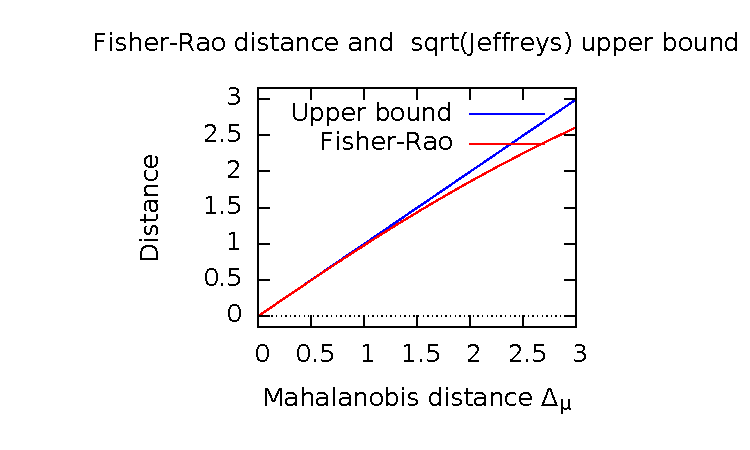
\includegraphics[width=0.7\columnwidth]{Plot-FRUBSameCovar.pdf}%
\caption{Quality of the $\sqrt{D_J}$ upper bound on the Fisher--Rao distance $\rho_\calN$ when normal distributions have the same covariance matrix.}%
\label{fig:ubsqrtJ}%
\end{figure}


For any smooth curve $c(t)$, we can thus approximate $\rho_\calN$ for large $T$ {by} %OK! style format. MDPI: We suggest deleting the lines around Equation (27)

\begin{equation}\label{eq:approx}
\boxed{\tilde\rho_\calN^c(N_1,N_2) := 
\frac{1}{T} \sum_{i=1}^{T-1} \sqrt{D_J\left[c\left(\frac{i}{T}\right),c\left(\frac{i+1}{T}\right)\right]}
.}
\end{equation}

For example, we may consider the following  curves on $\calM_{\calN}$ which admit closed-form parameterizations in $t\in[0,1]$:
\begin{itemize}
	\item linear interpolation (LERP, Linear intERPolation)
	$c_\lambda(t)=t (\mu_1,\Sigma_1)+(1-t)(\mu_2,\Sigma_2)$ 
	between $(\mu_1,\Sigma_1)$ and $(\mu_2,\Sigma_2)$,
	
	\item the mixture geodesic~\cite{nielsen2019jensen} $c_m(t)=\gamma^m_\calN(N_1,N_2;t)=(\mu_t^m,\Sigma_t^m)$ with
$\mu_t^m =\bar\mu_t$ and $\Sigma_t^m = \bar\Sigma_t+t\mu_1\mu_1^\top+(1-t)\mu_2\mu_2^\top-\bar\mu_t\bar\mu_t^\top$
where   $\bar\mu_t=t\mu_1+(1-t)\mu_2$ and $\bar\Sigma_t=t\Sigma_1+(1-t)\Sigma_2$,

\item the exponential geodesic~\cite{nielsen2019jensen} $c_e(t)=\gamma_\calN^e(N_1,N_2;t)=(\mu_t^e,\Sigma_t^e)$ with $\mu_t^e = \bar\Sigma_t^H (t\Sigma_1^{-1}\mu_1+(1-t)\Sigma_2^{-1}\mu_2)$
and $\Sigma_t^e =\bar\Sigma^H_t$
where $\bar\Sigma^H_t=(t\Sigma_1^{-1}+(1-t)\Sigma_2^{-1})^{-1}$ is the matrix harmonic mean,
\item the curve $c_{em}(t)=\frac{1}{2}\left(\gamma_\calN^e(N_1,N_2;t)+\gamma^m_\calN(N_1,N_2;t)\right)$ which is obtained by averaging the mixture geodesic with the exponential geodesic.
\end{itemize}

Figure~\ref{fig:vizemgeo2d} visualizes the exponential and mixture geodesics between two bivariate normal~distributions.

Let us denote by $\tilde\rho^{\lambda}_\calN=\tilde\rho^{c_\lambda}_\calN$,
 $\tilde\rho^{m}_\calN=\tilde\rho^{c_m}_\calN$, 
 $\tilde\rho^{e}_\calN=\tilde\rho^{c_e}_\calN$ and 
 $\tilde\rho^{em}_\calN=\tilde\rho^{c_{em}}_\calN$ the approximations obtained by these curves following from Equation~(\ref{eq:approx}).
When $T$ is sufficiently large, the~approximated distances $\tilde\rho^{x}$ are close to the length of curve $x$, and~we may thus consider a set of several curves $\{c_i\}_{i\in I}$ and report the smallest Fisher--Rao distance approximations obtained among these curves: 
$\rho_\calN(N_1,N_2)\approx \min_{i\in I} \tilde\rho_\calN^{c_i}(N_1,N_2)$. 

\begin{figure}[H]

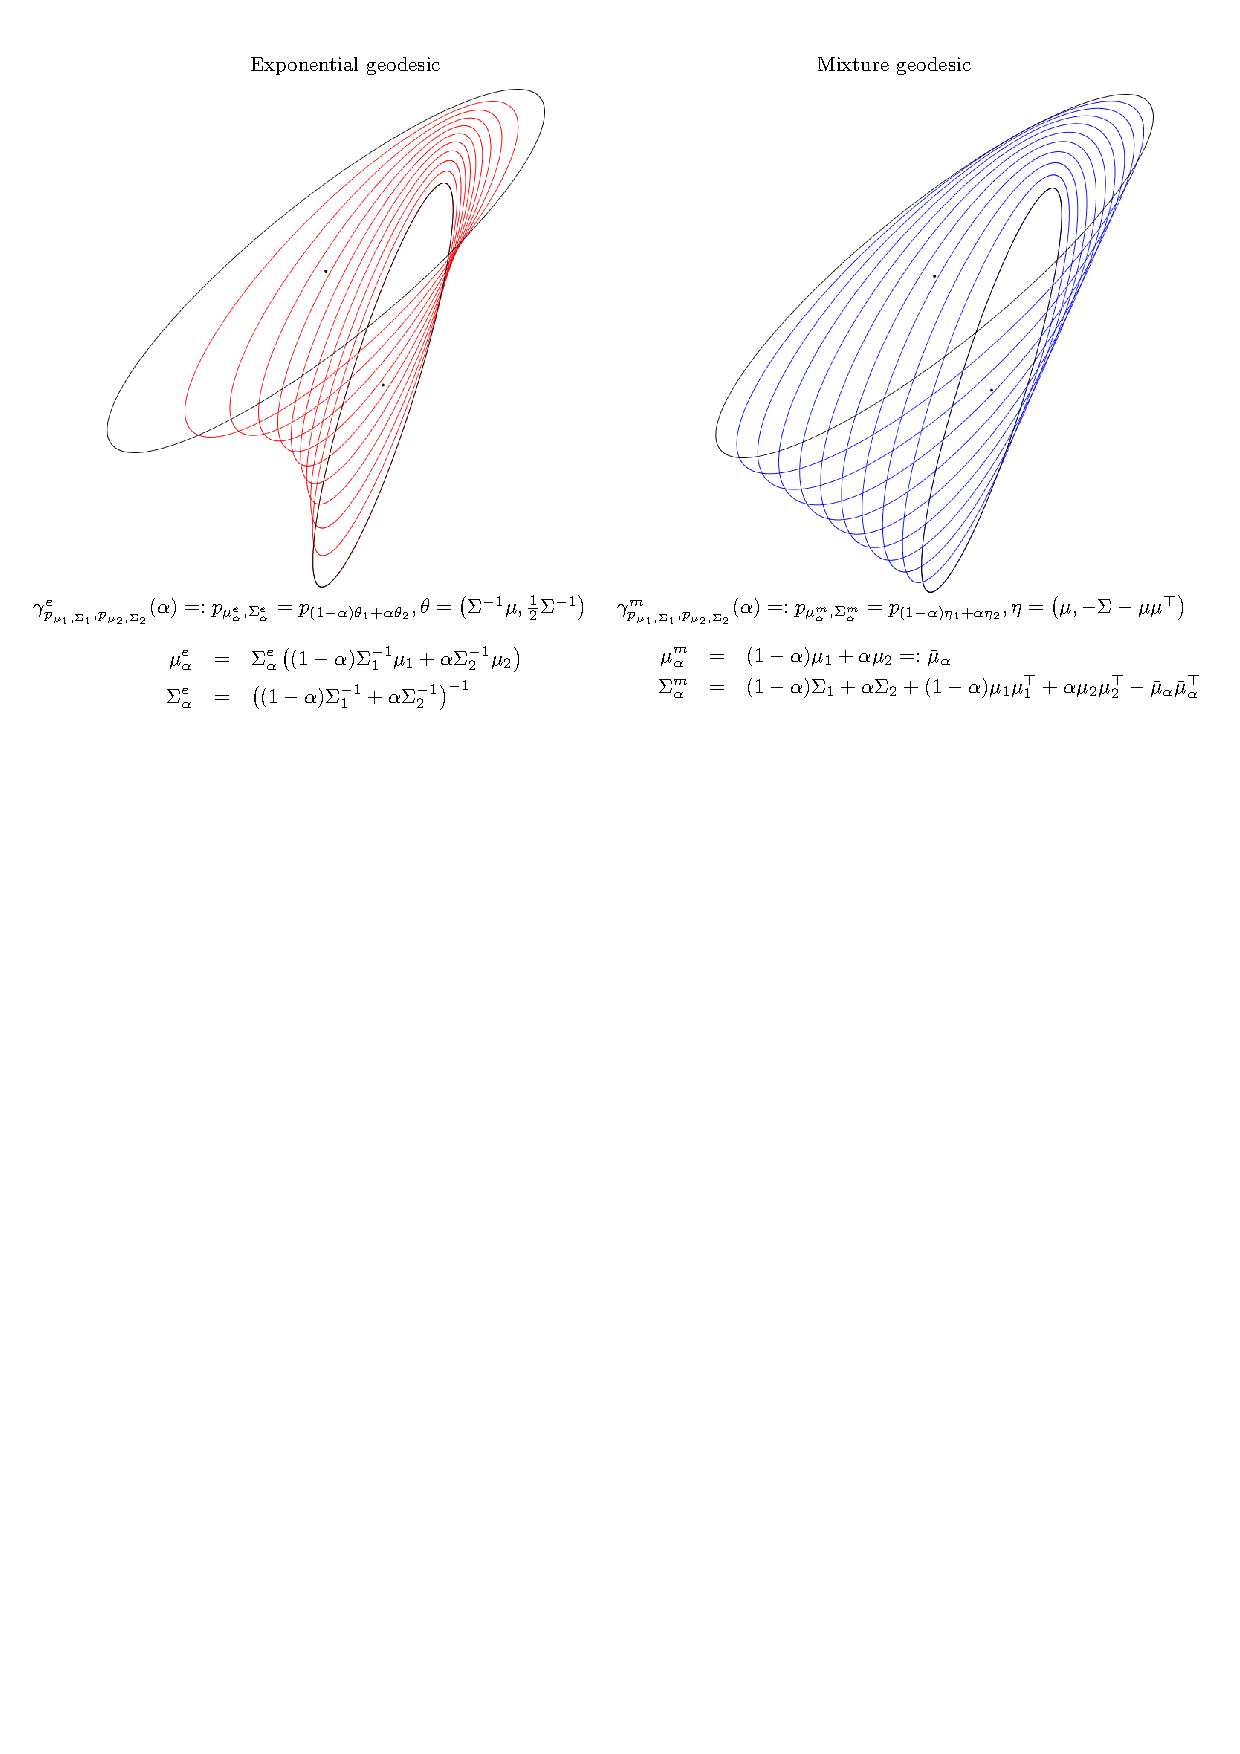
\includegraphics[width=0.95\textwidth]{FigIpe-BivariateInterpolation.pdf} 
\caption{\textls[-25]{Visualizing the exponential and mixture geodesics between two bivariate normal~distributions}.\label{fig:vizemgeo2d}}
\end{figure}



Please note that we consider the regular spacing for approximating a curve length and do not optimize the position of the sample points on the curve.
Indeed, as~$T\rightarrow\infty$, the~curve length approximation tends to the Riemannian curve length.
In other words,  we can measure approximately finely the length of any curve available with closed-form reparameterization by increasing $T$.
Thus, the key question of our method is how to best approximate the Fisher–Rao geodesic by a curve that can be parametrized by a closed-form formula and is close enough to the Fisher--Rao~geodesic.

Next, we introduce our approximation curve $c_\CO(t)$ derived from Calvo and Oller isometric mapping $f$ which experimentally behaves better when normals are not {\it too far} from each other.

%%%
\subsection{A Curve Derived from Calvo and Oller's~Embedding}\label{sec:cocurve}
%%%
This approximation consists of leveraging the closed-form expression of the SPD geodesics~\cite{moakher2011riemannian,RieMinimax-2013}: 
$$
\gamma_\calP(P,Q;t)=P^{\frac{1}{2}} \, \left(P^{-\frac{1}{2}}Q^{\frac{1}{2}}P^{-\frac{1}{2}}\right)^t \, P^{\frac{1}{2}},
\quad t\in[0,1]
$$ 
to approximate the Fisher–Rao normal geodesic $\gamma_\calN^\Fisher(N_1,N_2;t)$ as follows:
Let $\barP_1=f(N_1),\barP_2=f(N_2)\in\barN$, and~consider the smooth curve
\begin{equation}
\bar c_\CO(\barP_1,\barP_2;t)=\proj_{\barN}\left(\gamma_\calP(\barP_1,\barP_2;t)\right),
\end{equation}
where $\proj_{\barN}(P)$ denotes the orthogonal projection of $P\in\calP(d+1)$ onto $\barN$ ({Figure}~\ref{fig:projection}).
Thus, curve $c_\CO(t)$ ($t\in[0,1]$) is then defined by taking the inverse mapping $f^{-1}(\bar c_\CO)$  (Figure~\ref{fig:FRapprox}):
\begin{equation}
c_\CO(t)=f^{-1}\left(  \proj_{\barN}\left(\gamma_\calP(\barP_1,\barP_2;t)\right)  \right).
\end{equation}

Please note that the   matrix power $P^t$ can be computed as $P^t=U\,\diag(\lambda_1^t,\ldots,\lambda_d^t)\, V^\top$ where 
$P=U\,\diag(\lambda_1^t,\ldots,\lambda_d^t)\, V^\top $ is the eigenvalue decomposition of $P$.

\begin{figure}[H]

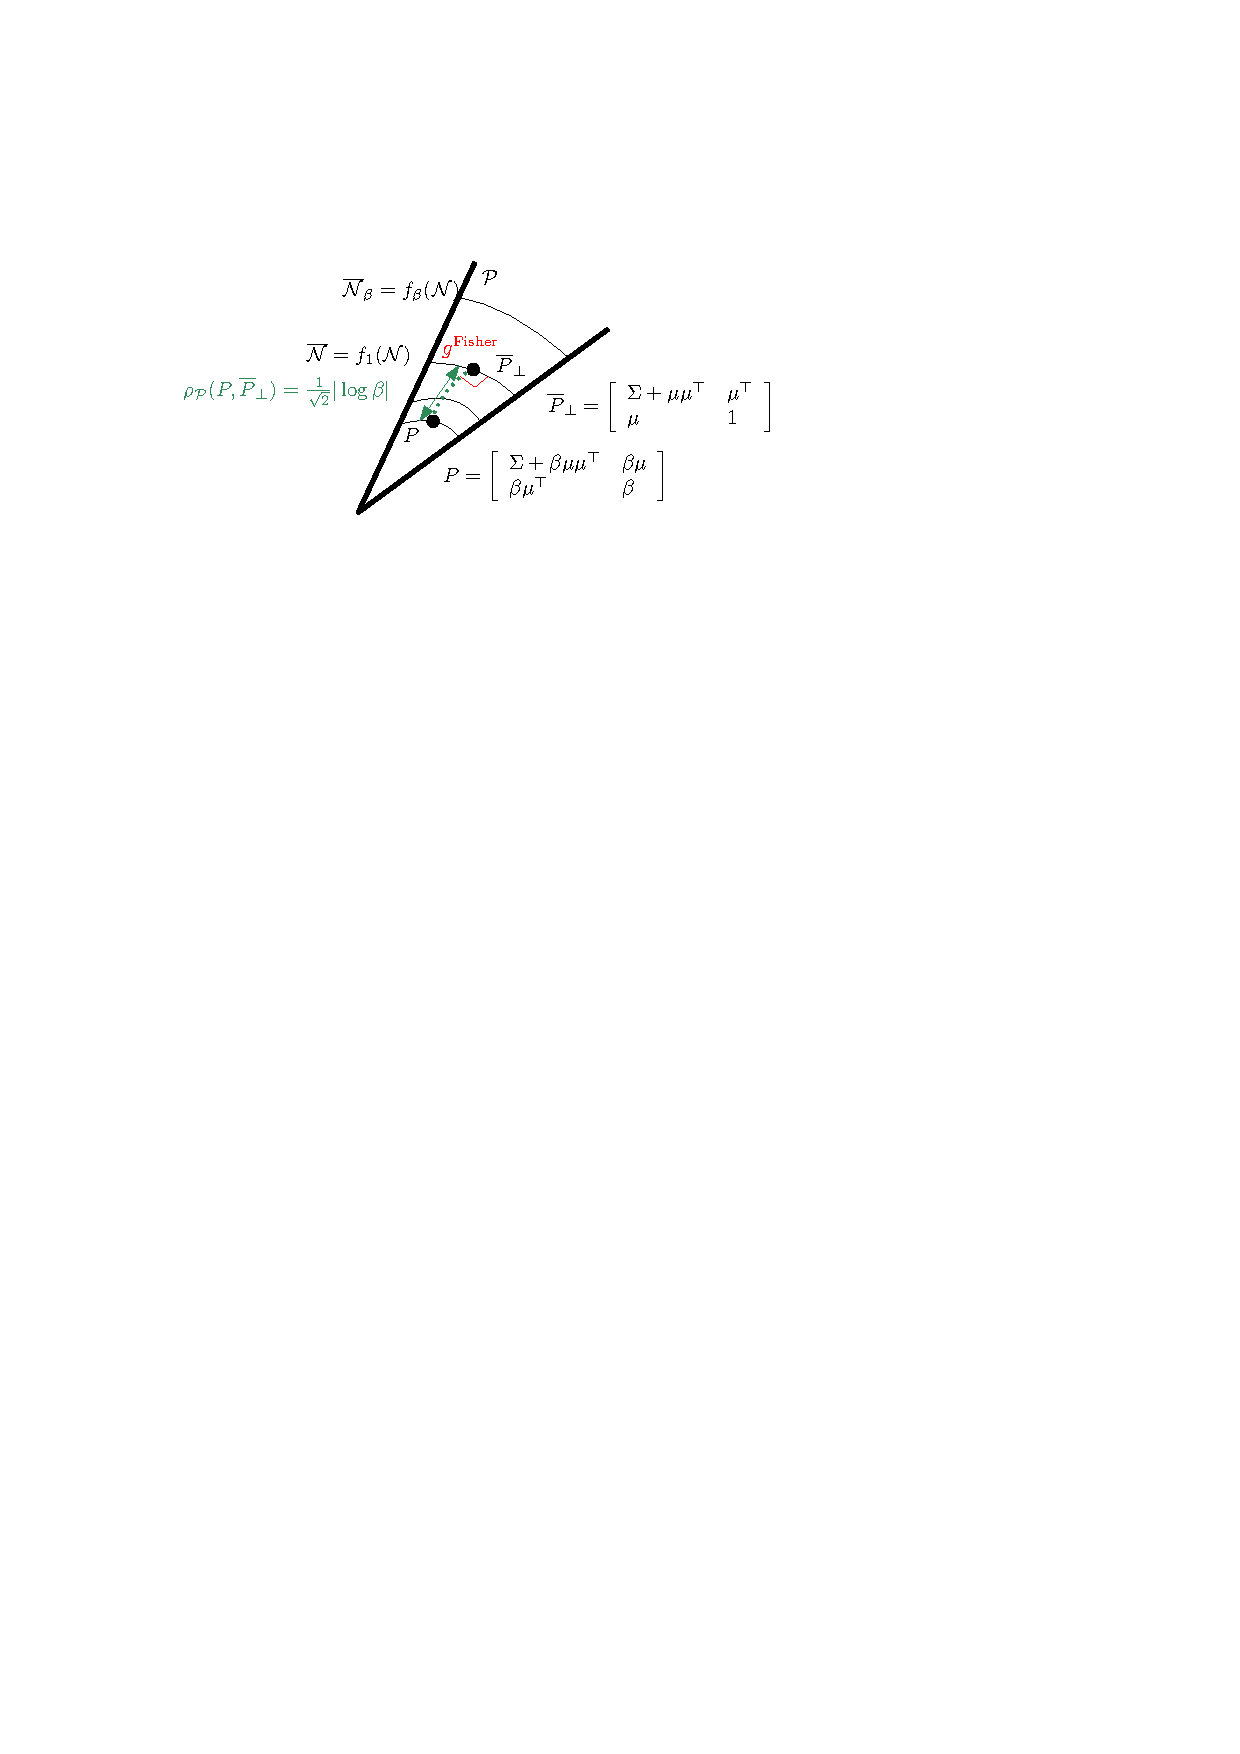
\includegraphics[width=0.65\textwidth]{FigIpe-OrthogonalProjectionSPD.pdf}
%
\caption{{Projecting} 
 an SPD matrix $P\in\calP$ onto $\barN=f(\calN)$: $\gamma_\calP(P,\barP_\perp)$ is orthogonal to $\barN$ with respect to the trace metric.
 \label{fig:projection}}
\end{figure}
 
Let us now explain how to project $P=[P_{i,j}]\in\calP(d+1)$ onto $\barN$ based on  the analysis of the Appendix of~\cite{SDPMVN-1990} (p. 239):

\begin{Proposition}[Projection of an SPD matrix onto the embedded normal submanifold $\barN$]\label{prop:proj}
Let $\beta=P_{d+1,d+1}$ and write  $P=\mattwotwo{\Sigma+\beta\mu\mu^\top}{\beta\mu}{\beta\mu^\top}{\beta}$.
Then the orthogonal projection at $P\in\calP$ onto $\barN$ is:
\begin{equation}
\barP_\perp:=\proj_{\barN}(P)=\mattwotwo{\Sigma+\mu\mu^\top}{\mu^\top}{\mu}{1},
\end{equation}
and the SPD distance between $P$ and $\barP_\perp$  is
\begin{equation}
\rho_\calP(P,\barP_\perp)=\frac{1}{\sqrt{2}} |\log\beta|.
\end{equation}
\end{Proposition}

Notice that the projection of $P$ is easily computed  since $\beta=P_{d+1,d+1}$.
$$
\proj_{\barN}\left(\mattwotwo{\Sigma+\beta\mu\mu^\top}{\beta\mu}{\beta\mu^\top}{\beta}\right)=\mattwotwo{\Sigma+\mu\mu^\top}{\mu^\top}{\mu}{1}
$$






\begin{figure}[H]

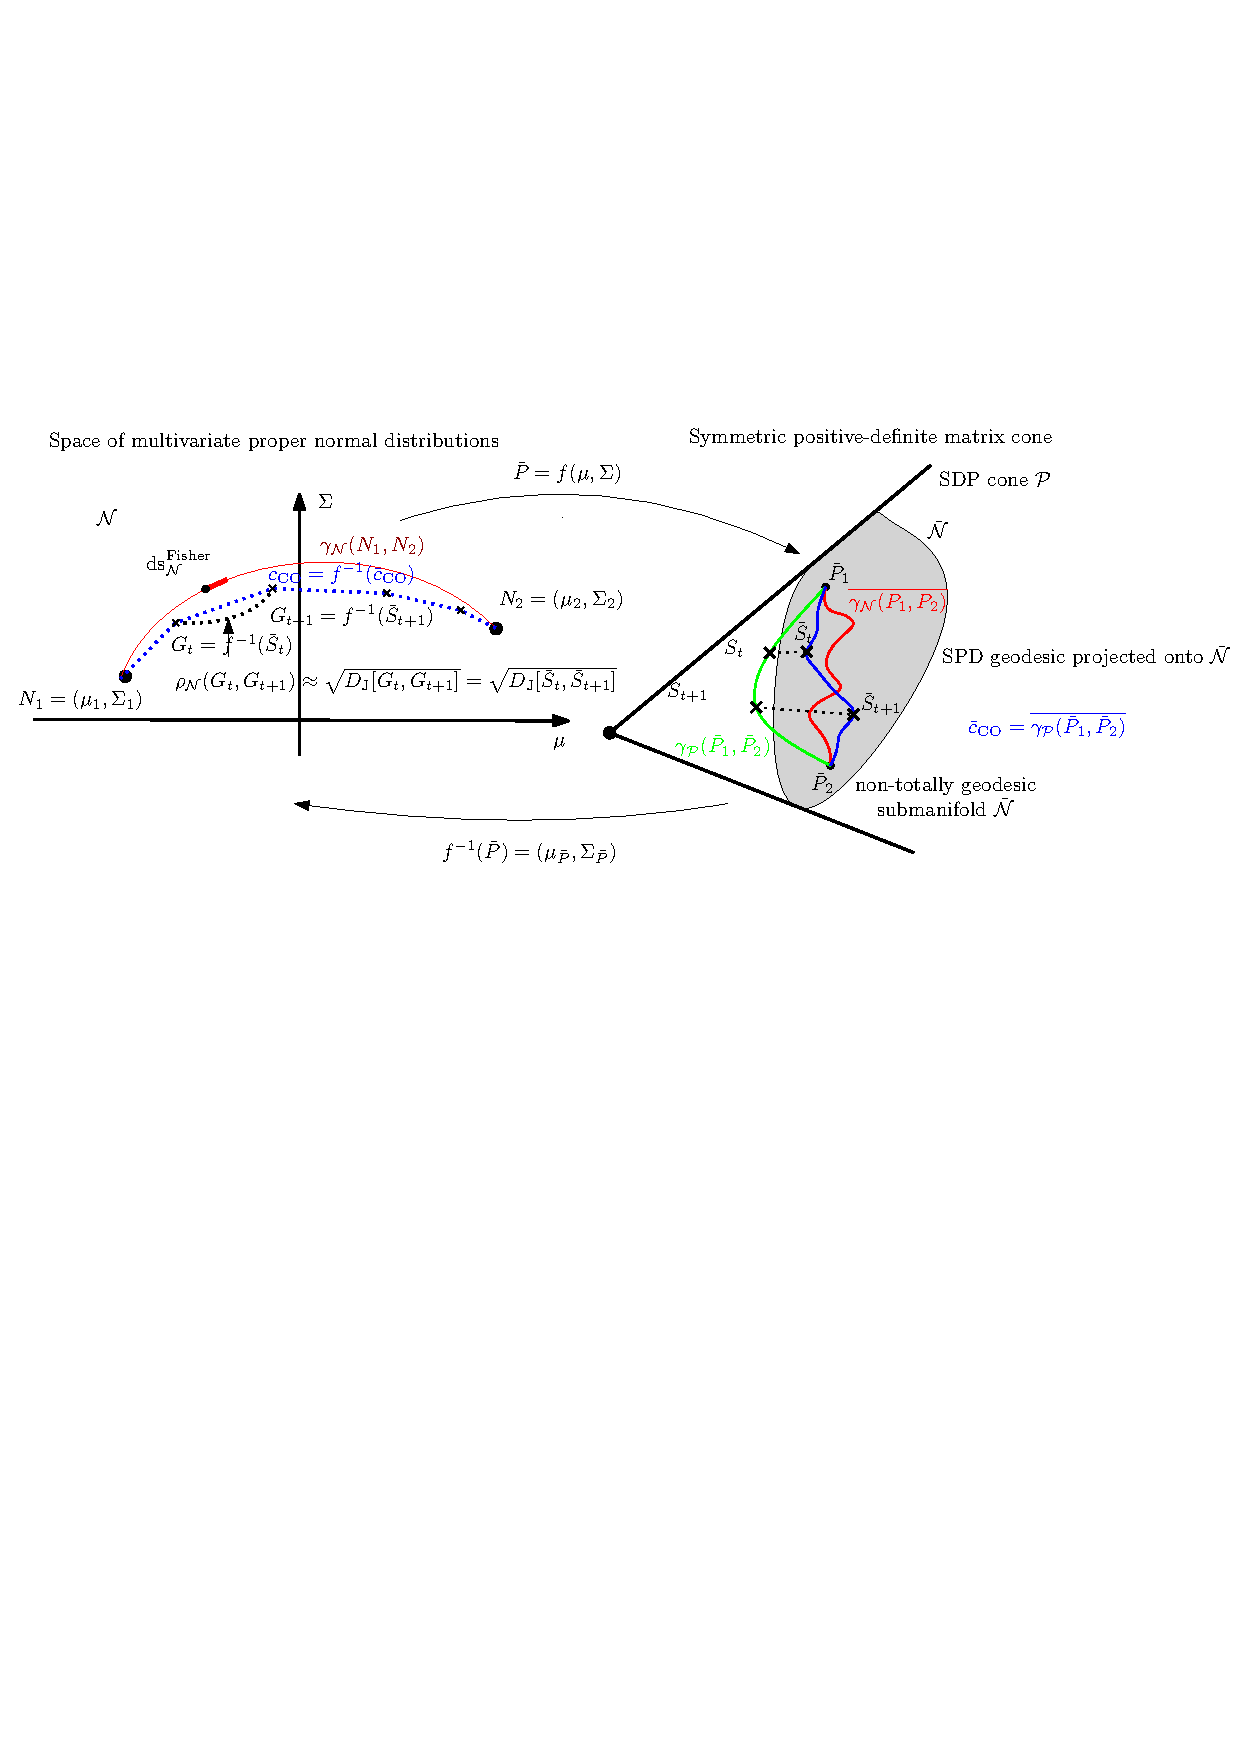
\includegraphics[width=0.85\textwidth]{FigIpe-ApproxFRMVN.pdf}
%
\caption{{Illustration} 
 of the approximation of the Fisher–Rao distance between two multivariate normals $N_1$ and $N_2$ (red geodesic length $\gamma_{\mathcal{N}}(N_1,N_2)$ by discretizing curve $\bar c_\CO\in\barN$ or equivalently curve $c_\CO\in\calN$.
 \label{fig:FRapprox}}
\end{figure}



\begin{Remark}
In Diffusion Tensor Imaging~\cite{MVNGeodesicShooting-2014} (DTI), 
the Fisher–Rao distance can be used to evaluate the distance between three-dimensional normal distributions with means located at a 3D grid position.
We may consider $3\times 3\times 3-1=26$ neighbor graphs induced by the grid, and~for each normal $N$ of the grid, calculate the approximations of the Fisher–Rao distance of $N$ with its neighbors $N'$ as depicted in Figure~\ref{fig:gridN}. 
Then the distance between two tensors $N_1$ and $N_2$ of the 3D grid is calculated as the shortest path on the weighted graph using Dijkstra's algorithm~\cite{MVNGeodesicShooting-2014}.
\end{Remark}

\begin{figure}[H]

\begin{tabular}{cc}
\fbox{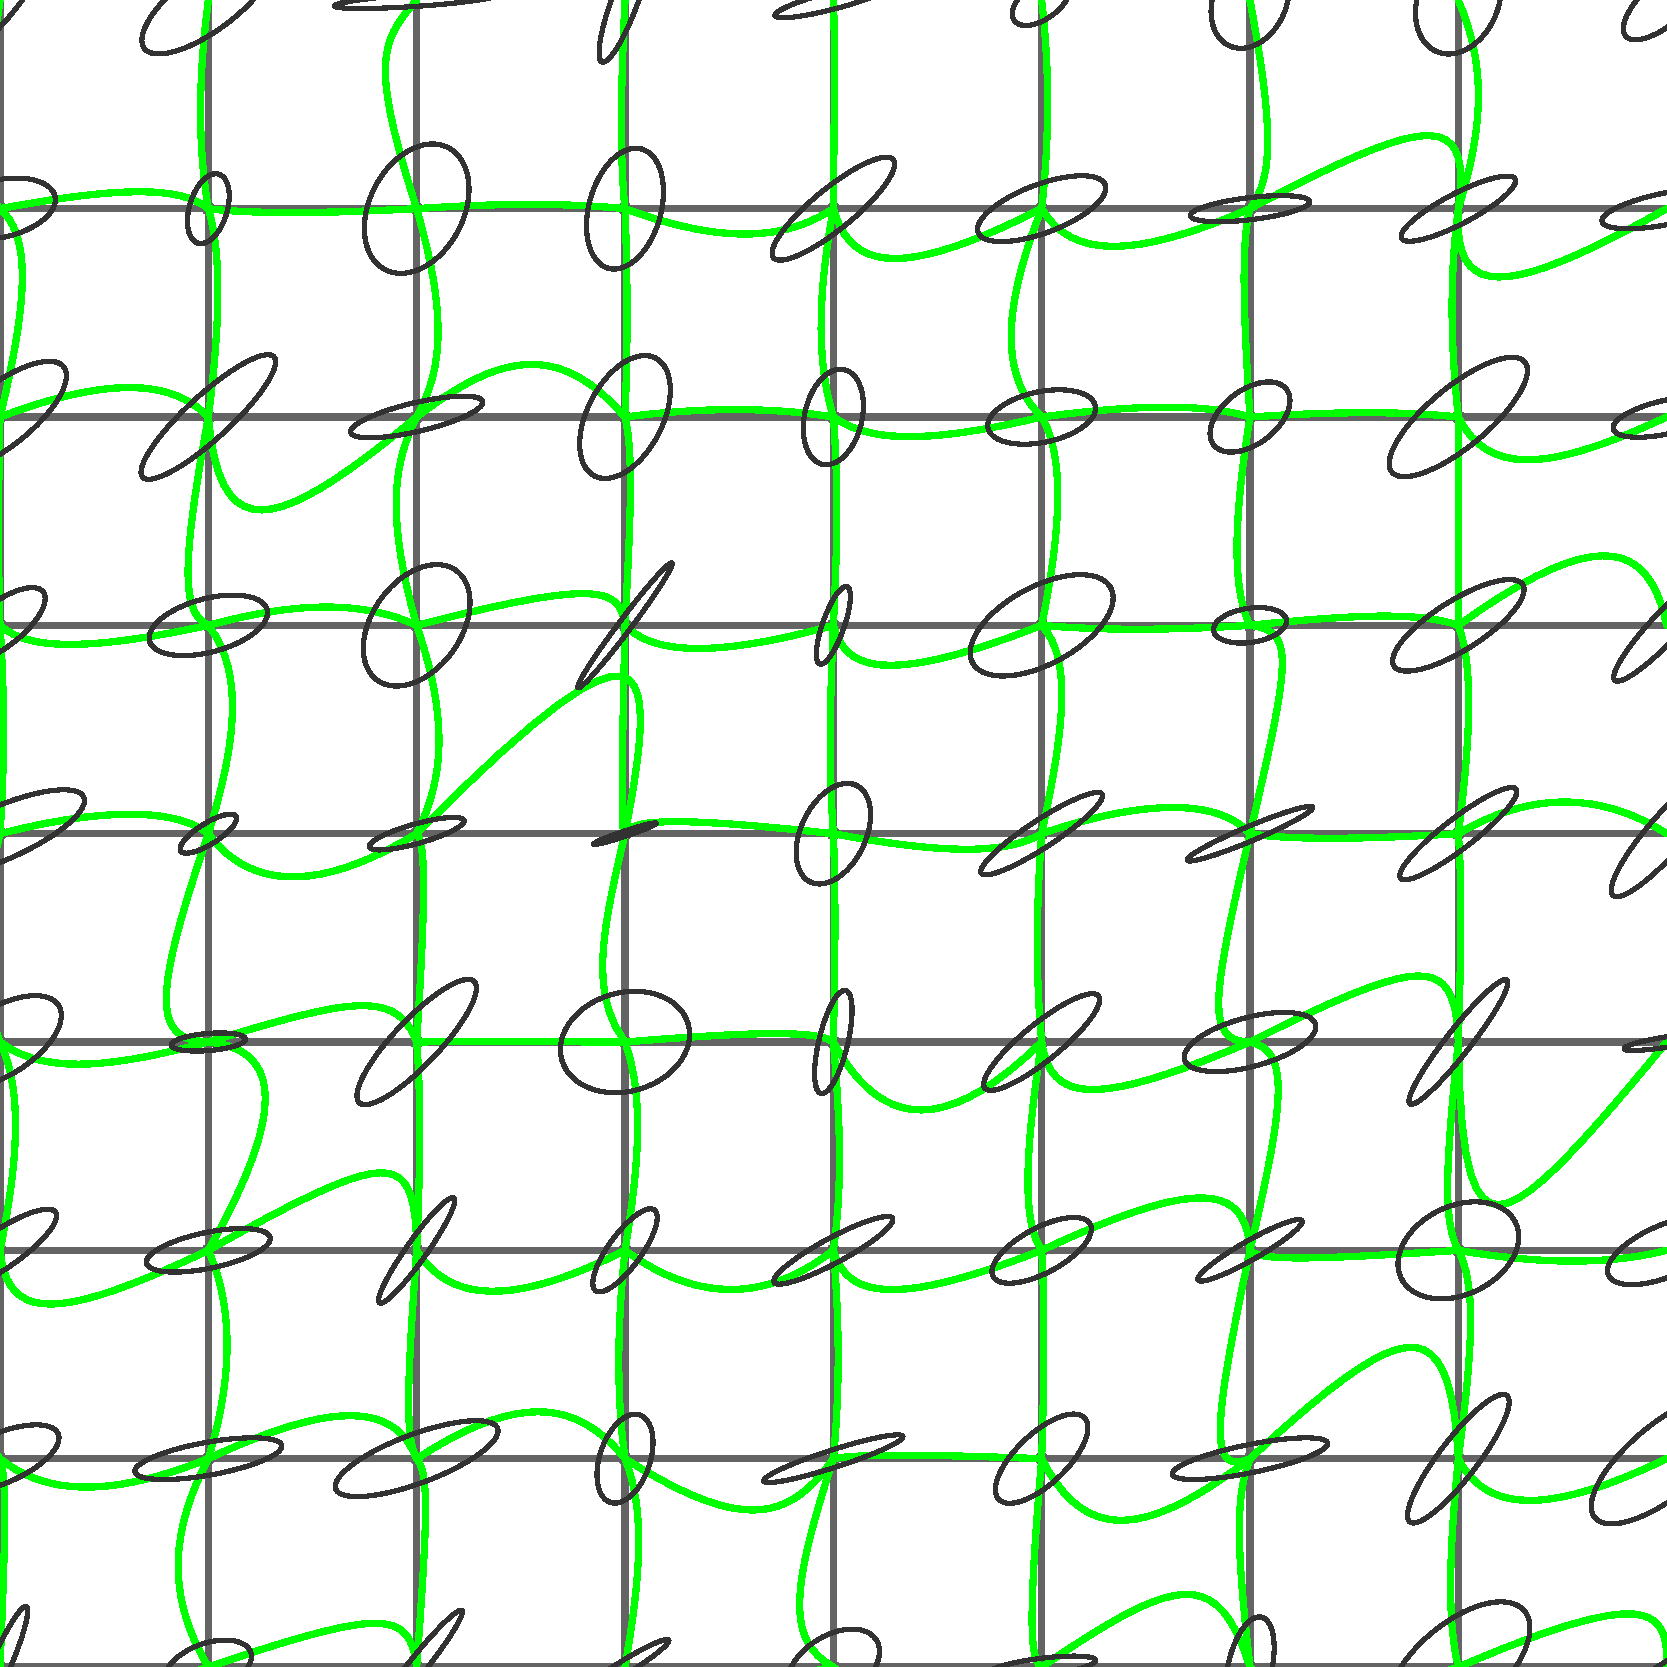
\includegraphics[width=0.33\textwidth]{2DgridN-geo.pdf}} &
\fbox{\includegraphics[width=0.33\textwidth]{2DgridN-geoEll.pdf}} \cr
(\textbf{a}) & (\textbf{b})
\end{tabular}
%
\caption{Diffusion tensor imaging (DTI) on a 2D grid: (\textbf{a}) Ellipsoids shown at the $8\times 8$ grid locations with C\&O curves in green, and~(\textbf{b}) some interpolated  ellipsoids are further shown along the C\&O curves.
 \label{fig:gridN}}
\end{figure}




Please note that the Fisher–Rao projection of $N_1=(\mu_1,\Sigma_1)$ onto a submanifold $\calM_{\mu_2}$ with fixed mean $\mu_2$ was recently reported in closed form in~\cite{tang2018information} {(Equation~(21)):} %Yes, it is of their paper. MDPI: Please check if Equation (21) belongs to Ref.72.

$$
N^*=N\left(\mu_2,\Sigma_1+\frac{1}{2}(\mu_2-\mu_1)(\mu_2-\mu_1)^\top\right),
$$
with
$$
\rho_\calN(N_1,N^*)=\frac{1}{\sqrt{2}}\, \arccosh\left(d+(\mu_2-\mu_1)^\top \Sigma_1^{-1} (\mu_2-\mu_1)\right),
$$
 and the Fisher–Rao projection of $N_1=(\mu_1,\Sigma_1)$ onto submanifold  $\calM_{\Sigma_2}$ is the
 ``vertical projection'' $N^*=(\mu_1,\Sigma_2)$ (Figure~\ref{fig:projsubmfds}) with
$$
\rho_\calN(N_1,N^*)=\rho_{\calN_\mu}(\Sigma_1,\Sigma_2).
$$

We can upper bound the Fisher–Rao distance $\rho_\calN((\mu_1,\Sigma_1),(\mu_2,\Sigma_2))$ by projecting $\Sigma_1$ onto $\calM_{\mu_2}$ and projecting $\Sigma_2$ onto $\calM_{\mu_1}$. Let $\Sigma_{12}\in\calM_{\mu_2}$ and $\Sigma_{21}\in\calM_{\mu_1}$ denote those Fisher–Rao orthogonal projections.
Using the triangular inequality property of the Fisher–Rao distance, we obtain the following upper bounds:
\begin{eqnarray}
\rho_\calN((\mu_1,\Sigma_1),(\mu_2,\Sigma_2)) &\leq & \rho_\calN((\mu_1,\Sigma_1),(\mu_2,\Sigma_{12}))
+\rho_\calN(\mu_2,\Sigma_{12},(\mu_2,\Sigma_{2})),\\
&\leq & \rho_\calN((\mu_2,\Sigma_2),(\mu_1,\Sigma_{21}))+\rho_\calN((\mu_1,\Sigma_{21}),(\mu_1,\Sigma_{1})).
\end{eqnarray}
See Figure~\ref{fig:projti} for an~illustration.






\begin{figure}[H]

\begin{tabular}{cc}
\fbox{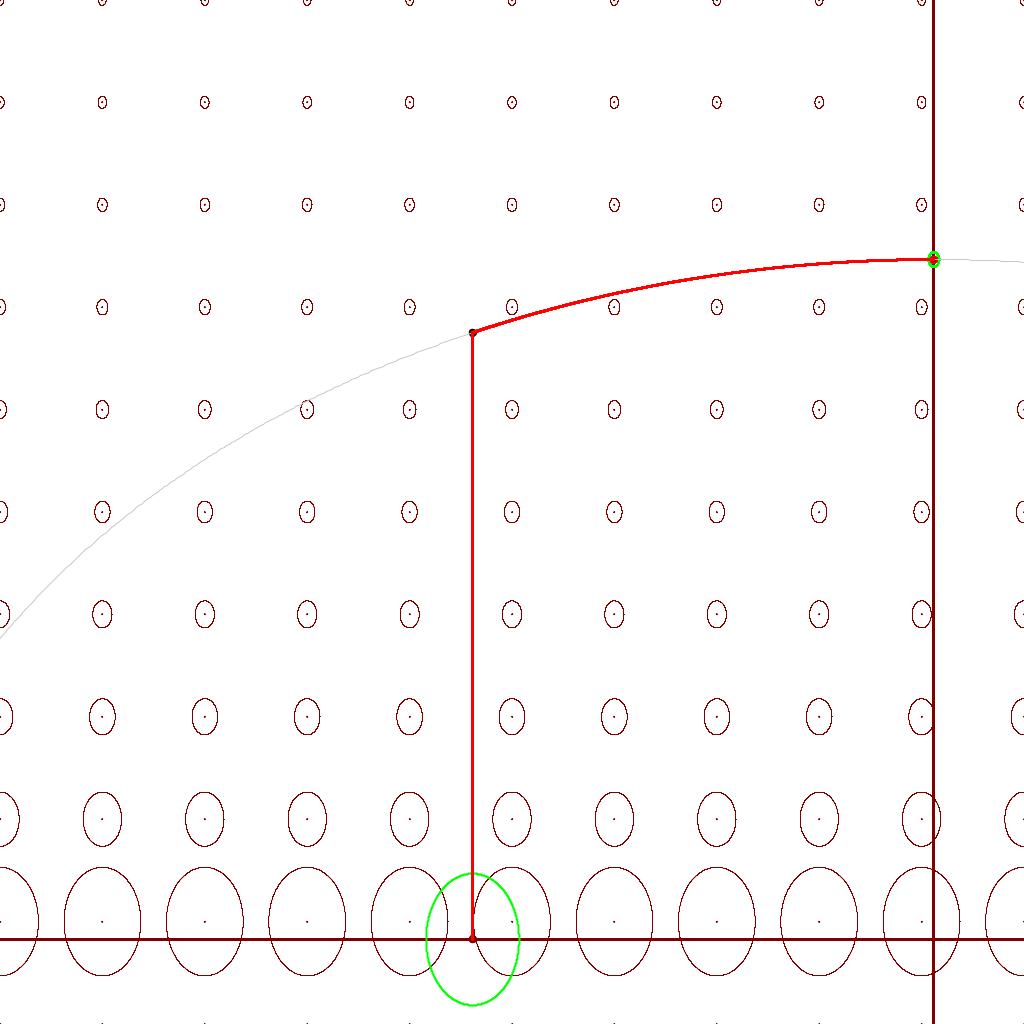
\includegraphics[width=0.33\textwidth]{Fig-ProjectionSubMfd1.png}} &
\fbox{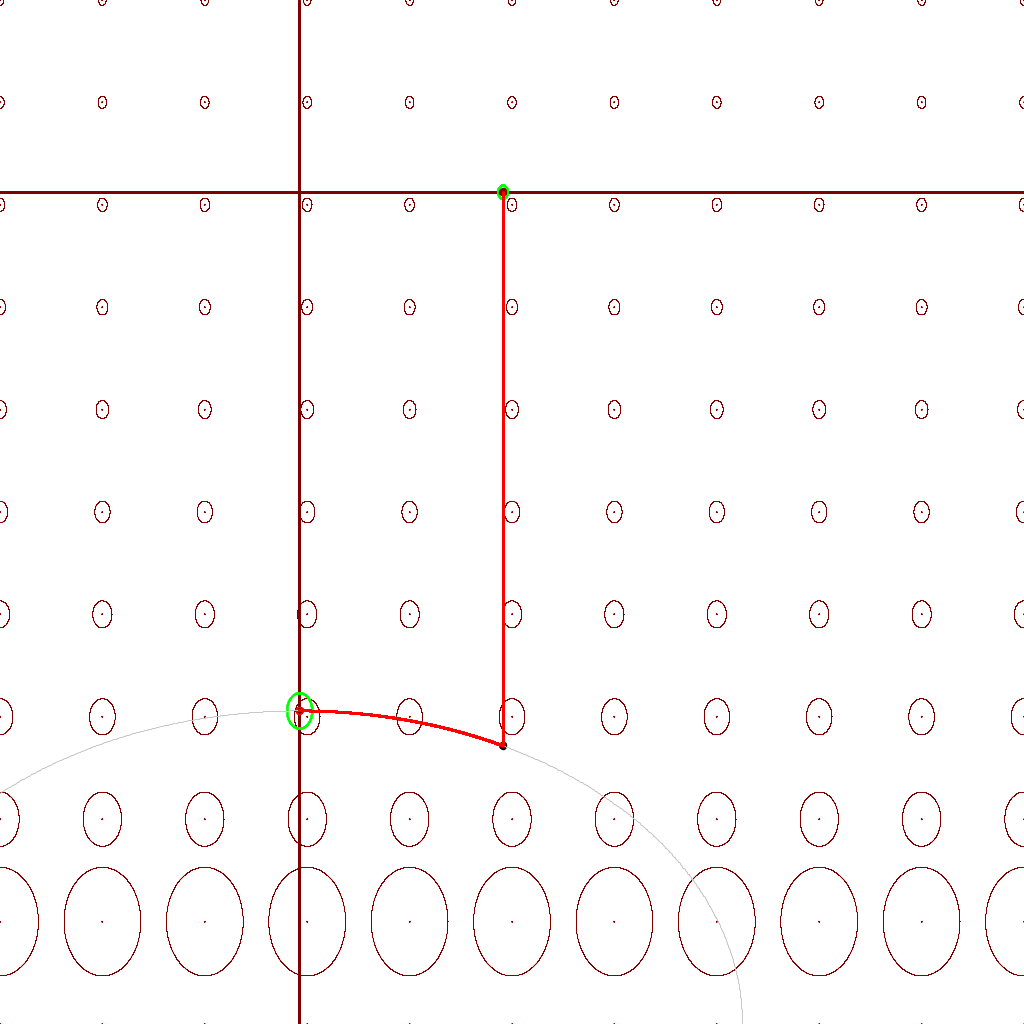
\includegraphics[width=0.33\textwidth]{Fig-ProjectionSubMfd2.png}}
\end{tabular}
\caption{Examples of projection of $N(\mu,\Sigma)$ onto the submanifolds $\calM_{\mu_0}$ and $\calM_{\Sigma_0}$.
Tissot indicatrices are rendered in green at the projected normal distributions 
$\left(\mu_0,\Sigma+\frac{1}{2}(\mu_0-\mu)(\mu_0-\mu)^\top\right)$ and $(\mu,\Sigma_0)$, respectively.}\label{fig:projsubmfds}
\end{figure}

\begin{figure}[H]

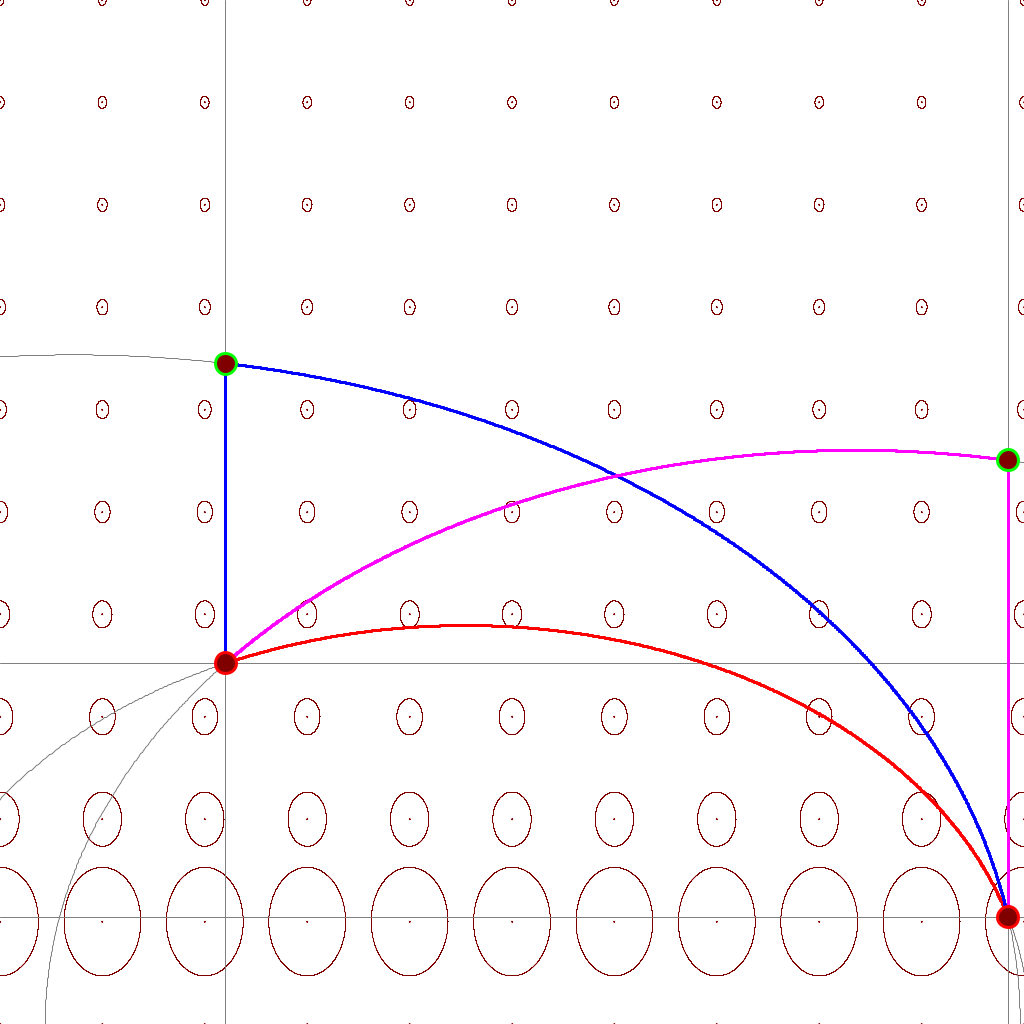
\includegraphics[width=0.35\textwidth]{Fig-ProjectionTriangularInequality.png}
\caption{Upper bounding the Fisher–Rao's distance $\rho_\calN((\mu_1,\Sigma_1),(\mu_2,\Sigma_2))$ (red points) using projections (green points) onto submanifolds with fixed~means.}\label{fig:projti}
\end{figure}
\unskip

Let $\bar c_\CO(t)=\bar S_t$ and $c_\CO(t)=f^{-1}(c_\CO(t))=:G_t$.
The following proposition shows that we have $D_J[\bar S_t,\bar S_{t+1}]=D_J[G_t,G_{t+1}]$.

\begin{Proposition}\label{prop:KL}
The Kullback–Leibler divergence   between 
$p_{\mu_1,\Sigma_1}$ and $p_{\mu_2,\Sigma_2}$ amounts to the KLD
between $q_{\bar P_1}=p_{0,f(\mu_1,\Sigma_1)}$ and $q_{\bar P_2}=p_{0,f(\mu_2,\Sigma_2)}$ where $\bar P_i=f(\mu_i,\Sigma_i)$:
$$
D_\KL[p_{\mu_1,\Sigma_1}:p_{\mu_2,\Sigma_2}]=D_\KL[q_{\bar P_1}:q_{\bar P_2}].
$$
\end{Proposition}





The KLD between two centered $(d+1)$-variate normals $q_{P_1}=p_{0,P_1}$ and $q_{P_2}=p_{0,P_2}$ is
$$
D_\KL[q_{P_1}:q_{P_2}]
=\frac{1}{2}\left(
\tr(P_2^{-1}P_1)-d-1+\log\frac{|P_2|}{|P_1|}
\right).$$
This divergence can be interpreted as the matrix version of the Itakura–Saito divergence~\cite{davis2006differential}.
The SPD cone equipped with $\frac{1}{2}$ of the trace metric can be interpreted as Fisher–Rao centered normal manifolds: 
$(\calN_\mu,g^\Fisher_{\calN_\mu})=(\calP,\frac{1}{2}g^\trace)$.

Since the determinant of a block matrix is
$$
\left|\mattwotwo{A}{B}{C}{D}\right|=\left|A-BD^{-1}C\right|,
$$
 we obtain with $D=1$: $|f(\mu,\Sigma)| = |\Sigma+\mu\mu^\top-\mu\mu^\top|=|\Sigma|$.

Let $\bar P_1=f(\mu_1,\Sigma_1)$ and 
$\bar P_2=f(\mu_2,\Sigma_2)$.
Checking $D_\KL[p_{\mu_1,\Sigma_1}:p_{\mu_2,\Sigma_2}]=D_\KL[q_{\bar P_1}:q_{\bar P_2}]$ where $q_{\barP}=p_{0,\barP}$ amounts to verify that
$$
\tr(\bar P_2^{-1}\bar P_1)=1+\tr(\Sigma_2^{-1}\Sigma_1+\Delta_\mu^\top\Sigma_2^{-1}\Delta_\mu).
$$
Indeed, using the inverse matrix  
$$f(\mu,\Sigma)^{-1}=
\mattwotwo{\Sigma^{-1}}{-\Sigma^{-1}\mu}{-\mu^\top\Sigma^{-1}}{1+\mu^\top \Sigma^{-1}\mu}
,$$
we have 
\begin{eqnarray*}
\tr(\bar P_2^{-1}\bar P_1)&=&\tr\left(
\mattwotwo{\Sigma^{-1}_2}{-\Sigma^{-1}_2\mu_2}{-\mu_2^\top\Sigma_2^{-1}}{1+\mu_2^\top \Sigma^{-1}_2\mu_2}\ \mattwotwo{\Sigma_1+\mu_1\mu_1^\top}{\mu_1}{\mu_1^\top}{1}
\right),\\
&=& 1+\tr(\Sigma_2^{-1}\Sigma_1+\Delta_\mu^\top\Sigma_2^{-1}\Delta_\mu).
\end{eqnarray*}
Thus, even if the dimension of the sample spaces of $p_{\mu,\Sigma}$ and $q_{\barP=f(\mu,\Sigma)}$ differs by one, we obtain the same KLD by Calvo and Oller's isometric mapping $f$.
 

This property holds for the KLD/Jeffreys divergence $D_J$ but not for all $f$-divergences~\cite{IG-2016} $I_f$ in general (e.g., it fails for the Hellinger divergence).

Figure~\ref{Fig:CurvesTissot} shows the various geodesics and curves used to approximate the Fisher–Rao distance with the Fisher metric shown using Tissot~indicatrices.
\begin{figure}[H]

\begin{tabular}{ccc}
\fbox{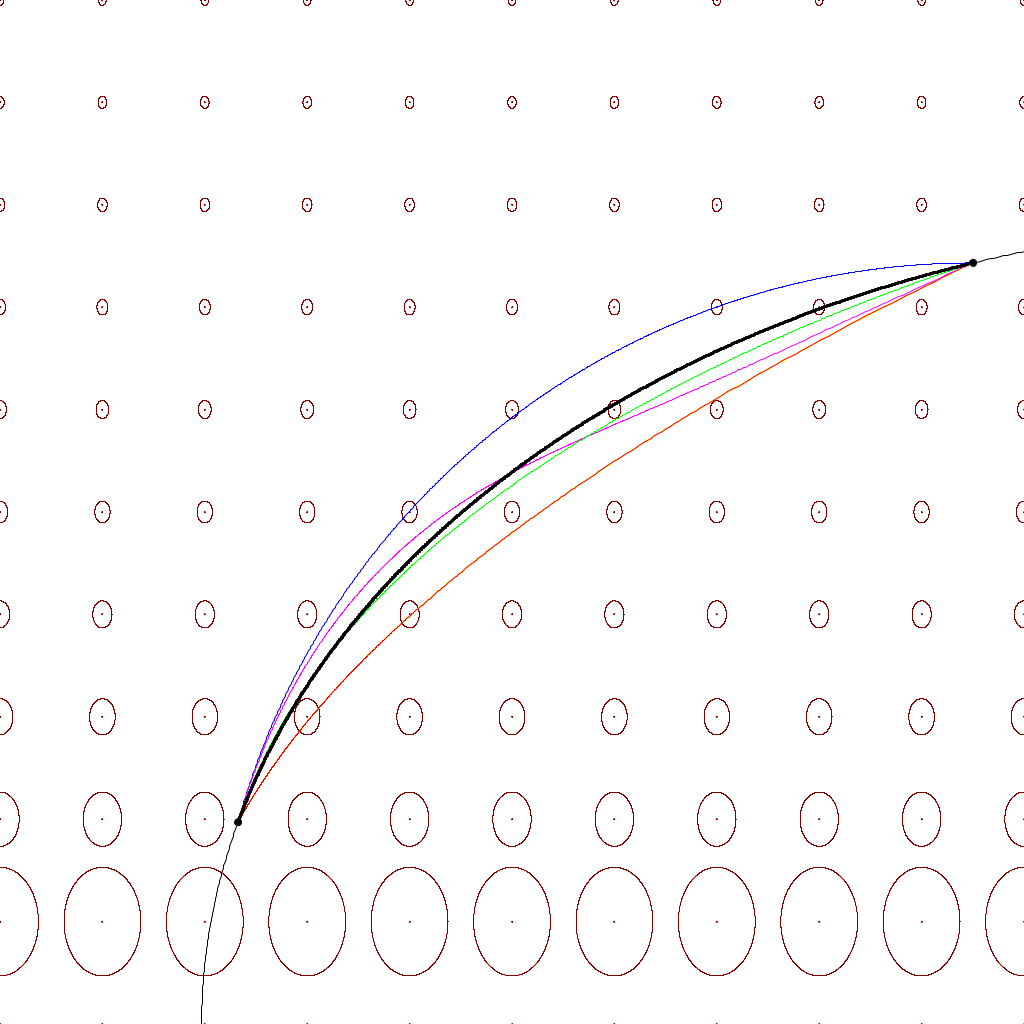
\includegraphics[width=0.23\textwidth]{UnivariateNormal-Tissot1.png}} &
\fbox{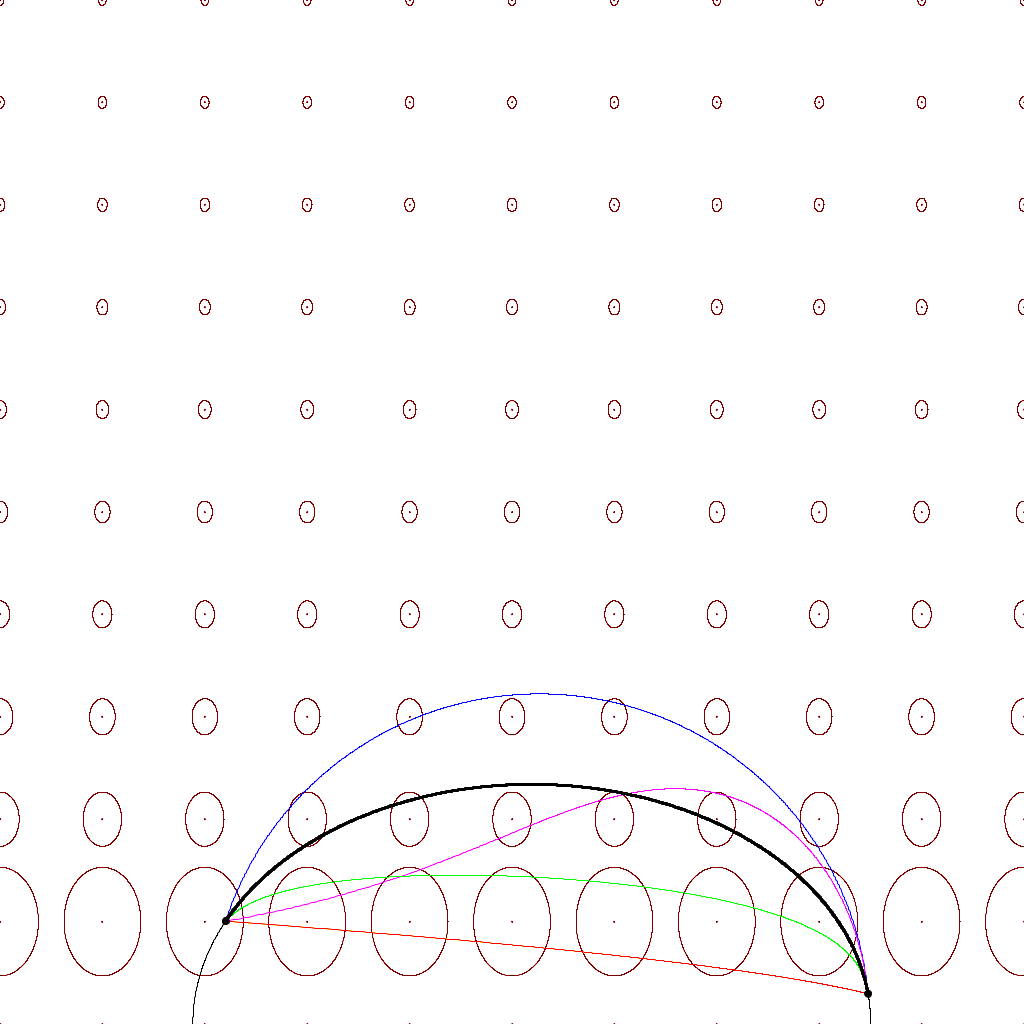
\includegraphics[width=0.23\textwidth]{UnivariateNormal-Tissot2.png}} &
\fbox{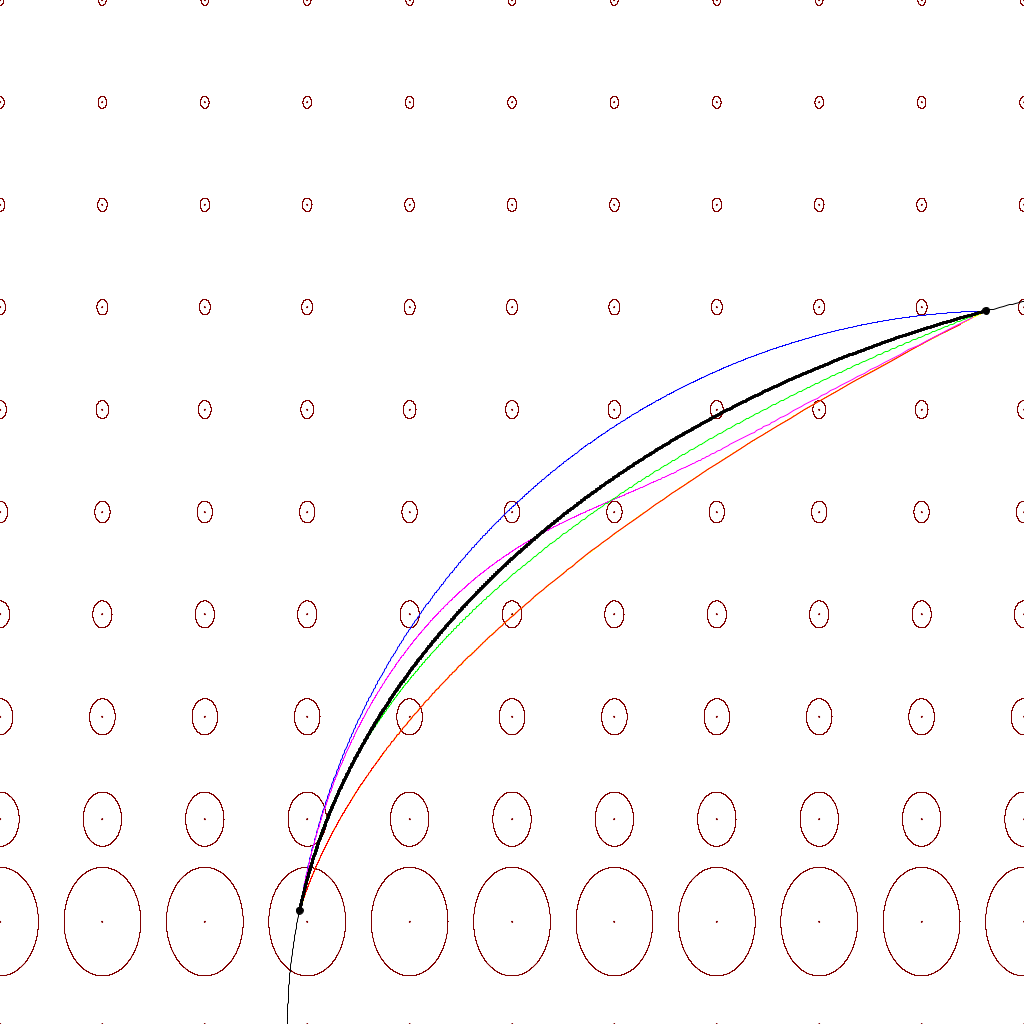
\includegraphics[width=0.23\textwidth]{UnivariateNormal-Tissot3.png}}
\end{tabular}
\caption{Geodesics and curves used to approximate the Fisher–Rao distance with the Fisher metric shown using Tissot's indicatrices:
exponential geodesic (red), mixture geodesic (blue), mid-exponential-mixture curve (purple), projected CO curve (green), and target Fisher–Rao geodesic (black). (Visualization in the parameter space of normal distributions).}\label{Fig:CurvesTissot}
\end{figure}



Please note that the introduction of parameter $\beta$ is related to the foliation of the SPD cone $\calP$ by $\{f_{\beta}(\calN) \st \beta>0\}$: $\calP(d+1)=\bbR_{>0}\times f_{\beta}(\calN)$. See {Figure}~\ref{fig:projection}.
Thus, we may define how good the projected C\&O curve is to the Fisher–Rao geodesic by measuring the average distance between points on $\gamma_\calP(\barP_1,\barP_2;t)$ and their projections $\overline{\gamma_\calP(\barP_1,\barP_2;t)}^\perp$ onto $\barN$:
$$
\delta^\CO(N_1,N_2)=\delta^\CO(\barP_1,\barP_2)=\int_0^1 \rho_\calP(\gamma_\calP(\barP_1,\barP_2;t),\overline{\gamma_\calP(\barP_1,\barP_2;t)}^\perp)\, \dt.
$$
In practice, we evaluate this integral at the sampling points $S_t$:
\begin{equation}\label{eq:avgprojdist}
\delta^\CO(P_1,P_2) \approx \delta^\CO_T(P_1,P_2):=\frac{1}{T}\sum_{i=1}^T  \rho_\calP(S_t,\bar{S}_t),
\end{equation}
\textls[-58]{where $S_t=\gamma_\calP(\barP_1,\barP_2;t)$ and $\bar{S}_t=\gamma_\calP(\barP_1,\barP_2;t)^\perp$.
We checked experimentally (see \mbox{Section~\ref{sec:exp}}) }
that for close by normals $N_1$ and $N_1$, we have $\delta^\CO(\bar{N}_1,\bar{N}_2)$ small, and~that when $N_1$ becomes further separated from $N_2$, the~average projection error $\delta^\CO(\bar{N}_1,\bar{N}_2)$ increases.
Thus, $\delta^\CO_T(P_1,P_2)$ is a good measure of the precision of our Fisher–Rao distance~approximation.

\begin{Lemma}\label{lemmati}
We have $\rho_{\barN}(\bar{S}_t,\bar{S}_{t+1})\leq \rho_\calP(\bar S_t,S_t)+\rho_\calP(S_t,S_{t+1})+\rho_\calP(S_{t+1},\bar S_{t+1})$.
\end{Lemma}

\begin{proof}
The proof consists of applying twice the triangle inequality of metric distance $\rho_\calP$:
\begin{eqnarray*}
\rho_{\barN}(\bar{S}_t,\bar{S}_{t+1}) &\leq&  \rho_\calP(\bar{S}_t,S_{t+1})+\rho_\calP(S_{t+1},\bar S_{t+1}),\\
&\leq &  \rho_\calP(\bar{S}_t,S_{t}) + \rho_\calP(S_t,S_{t+1}) + \rho_\calP(S_{t+1},\bar S_{t+1}).
\end{eqnarray*}
See Figure~\ref{fig:approxCO} where the left-hand-side geodesic length is shown in blue and the right-hand-side upper bound is visualized in red.
\end{proof}

\begin{figure}[H]

 
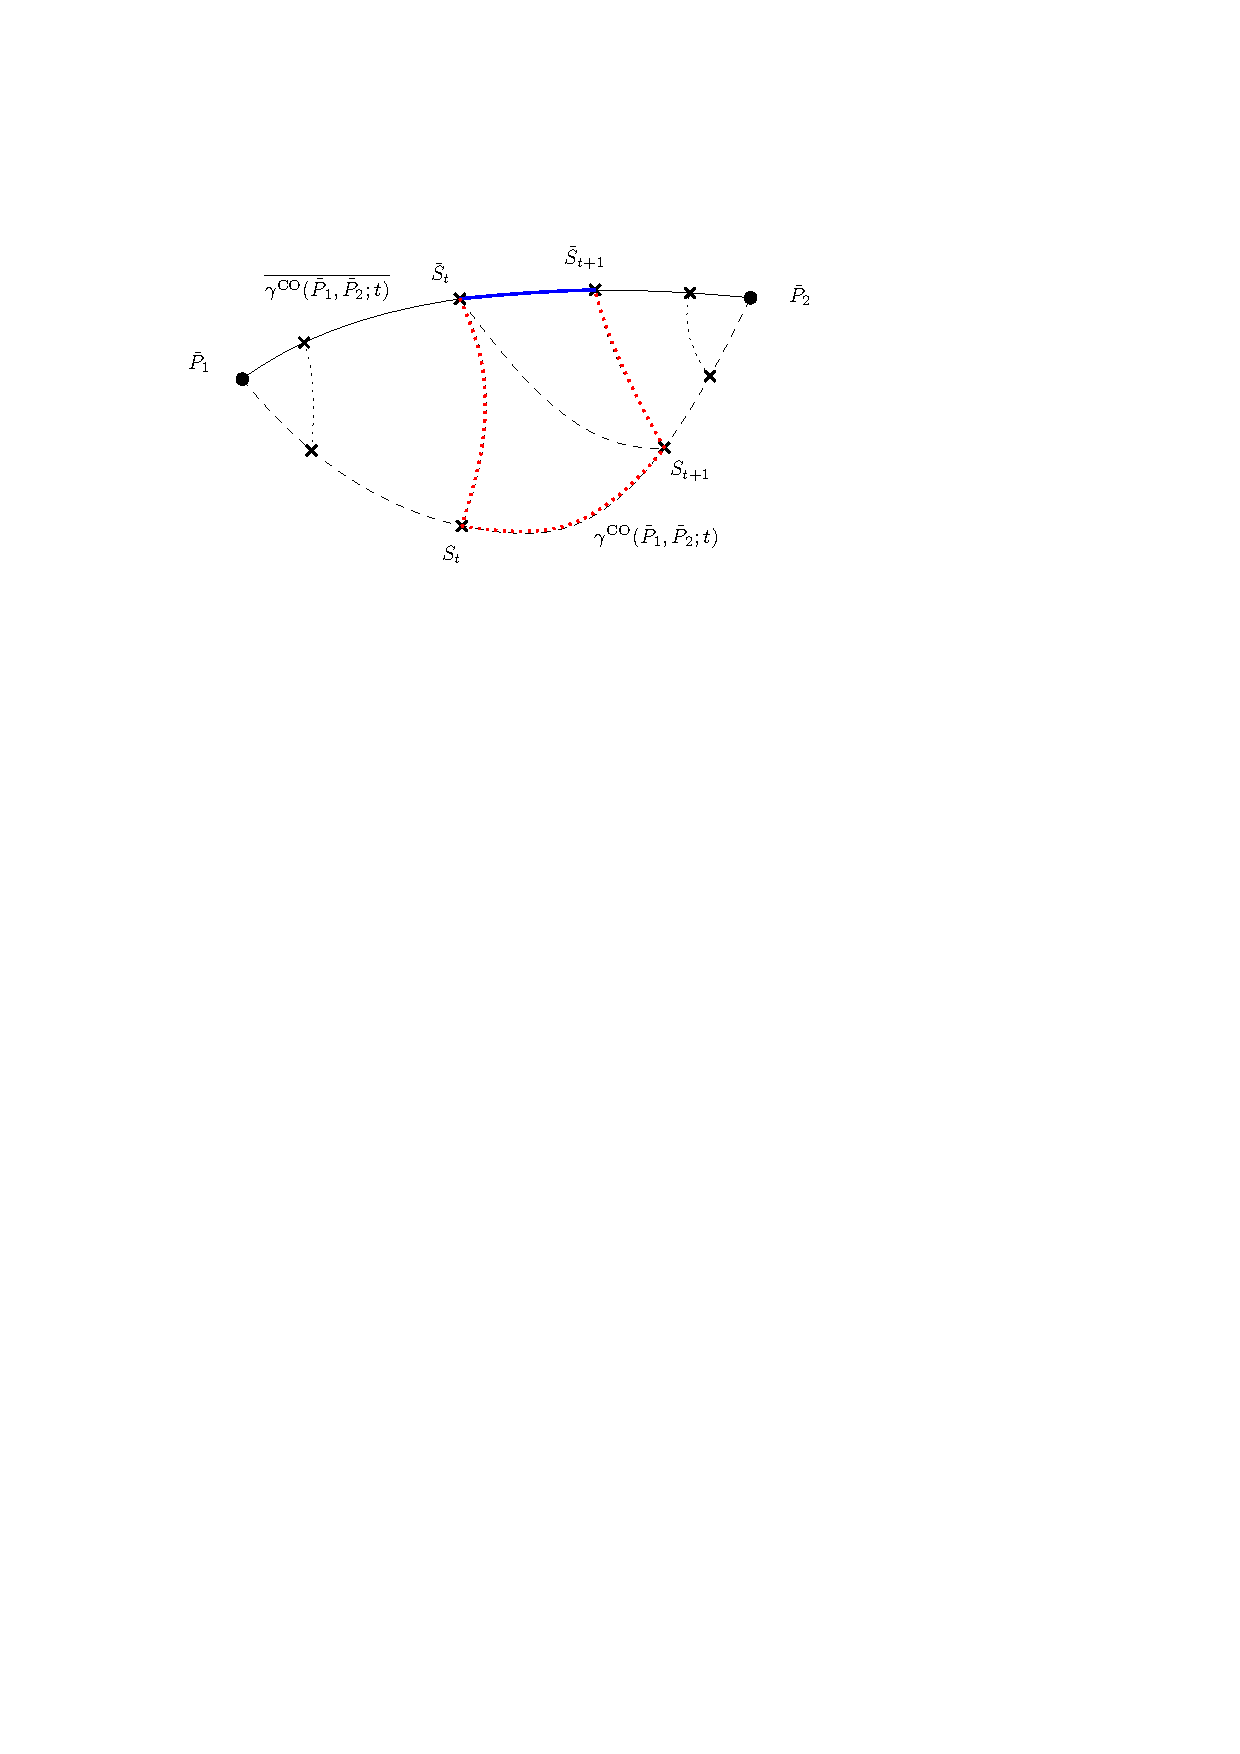
\includegraphics[width=0.5\textwidth]{FigIpe-ControlCOApproximation.pdf}  
 
%
\caption{Bounding $\rho_\calN(\bar S_t,\bar S_{t+1})$ using the triangular inequality of $\rho_\calP$ in the SPD cone $\calP(d+1)$.
 \label{fig:approxCO}}
\end{figure}

\begin{Property}
We have 
$\rho_\calN(N_1,N_2)\leq \rho_\calN^\CO(N_1,N_2) \leq  \rho_\calN(N_1,N_2) + 2\, \delta^\CO_T(\bar P_1,\bar P_2)$.
\end{Property}

\begin{proof}
At infinitesimal scale when $S_{t+1}\approx S_t$, using Lemma~\ref{lemmati} and $\rho_\calP(S_{t+1},\bar S_{t+1})\approx \rho_\calP(\bar S_t,S_t)$ we have
$$
\ds_{\calN}(\bar S_t) \leq \ds_{\calP}(S_t) + 2\rho_\calP(S_t,\bar S_t). 
$$

Taking the integral along the curve $c^\CO(t)=\overline{\gamma^\CO(\barP_1,\barP_2;t)}$, we obtain
$$
\rho_\calN^\CO(N_1,N_2)\leq \rho_\calP(\bar P_1,\bar P_2) + 2 \delta^\CO_T(\bar P_1,\bar P_2)
$$
Since $\rho_\calP(\barP_1,\barP_2)\leq \rho_\calN(N_1,N_2)$, we have
$$
\rho_\calN(N_1,N_2)\leq \rho_\calN^\CO(N_1,N_2) \leq  \rho_\calN(N_1,N_2) + 2 \delta^\CO_T(\bar P_1,\bar P_2).
$$
\end{proof}

Notice that $\sum_{i=0}^{T-1} \rho_\calP(S_t,S_{t+1})=\rho_\calP(\barP_1,\barP_2)$.

 
\begin{Example}\label{ex1entropy}
Let us consider Example~1 of~\cite{FRMVNReview-2020} (p. 11):
$$
N_1=\left(\vectortwo{-1}{0},\Sigma\right),\quad
N_2=\left(\vectortwo{6}{3},\Sigma\right), \Sigma=\mattwotwo{1.1}{0.9}{0.9}{1.1}.
$$
{The Fisher–Rao distance is evaluated numerically in~\cite{FRMVNReview-2020} as $5.00648$.
We have the lower bound $\rho_\calN^\CO(N_1,N_2)=4.20447$, and~the Mahalanobis distance $8.06226$ upper bounds the Fisher–Rao distance (not totally geodesic submanifold $\calN_\Sigma$).
Our projected C\&O curve discretized with $T=1000$ yields an approximation $\tilde\rho_\calN^\CO(N_1,N_2)=5.31667$.
The average projection distance $\rho_\calP(S_t,\bar S_{t})$ is $\delta^\CO_T(N_1,N_2)=0.61791$, and~the maximum projected distance is $1.00685$.
We check that}
$$
5.00648\approx \rho_\calN(N_1,N_2)\leq \tilde\rho_\calN^\CO(N_1,N_2)\approx 5.31667 \leq \rho_\calN(N_1,N_2) + 2 \delta^\CO_T(\bar P_1,\bar P_2)\approx 5.44028.
$$
The Killing distance~\cite{lovric2000multivariate} obtained for $\kappa_\Killing=2$ is $\rho_\Killing(N_1,N_2)\approx 6.82028$ (see Appendix~\ref{sec:SS}).
Notice that geodesic shooting is time-consuming compared to our approximation technique.
\end{Example}
 
 
 
%%%%
\subsection{Some~Experiments}\label{sec:exp}
%%%%

The KLD $D_\KL$ and Jeffreys divergence $D_J$, the~Fisher–Rao distance $\rho_\calN$ and the Calvo and Oller distance $\rho_\CO$ are all invariant under the congruence action of the affine group $\Aff(d)=\bbR^d\rtimes\GL(d)$ with the group operation 
$$
(a_1,A_1)(a_2,A_2)=(a_1+A_1a_2,A_1A_2).
$$
Let $(A,a)\in\Aff(d)$, and~define the action on the normal space $\calN$ as follows:
$$
(A,a).N(\mu,\Sigma)=N(A^\top\mu+a,A\Sigma A^\top).
$$
Then we have:
\begin{eqnarray*}
\rho_{\calN}((A,a).N_1,(A,a).N_2)&=& \rho_{\calN}(N_1,N_2),\\
\rho_{\CO}((A,a).N_1,(A,a).N_2)&=&\rho_{\CO}(N_1,N_2),\\ 
D_\KL[(A,a).N_1:(A,a).N_2]&=&D_\KL[N_1:N_2].
\end{eqnarray*}
This invariance extends to our approximations $\tilde\rho^c_\calN$ (see Equation~(\ref{eq:approx})).
 
Since we have 
$$
\tilde\rho_{\calN}^c(N_1,N_2)\approx \rho_{\calN}(N_1,N_2)\geq \rho_{\CO}(N_1,N_2),
$$
the ratio $\kappa_c=\frac{\tilde\rho_{\calN}^c}{\rho_{\CO}}\geq \kappa=\frac{\tilde\rho_{\calN}^c}{\rho_{\calN}}$ gives an upper bound on the approximation factor of $\tilde\rho_{\calN}^c$ compared to the true Fisher–Rao distance $\rho_{\calN}$:
$$
\kappa_c \rho_{\calN}(N_1,N_2)\geq \kappa \rho_{\calN}(N_1,N_2)\geq \tilde\rho_{\calN}^c(N_1,N_2)\approx \rho_{\calN}(N_1,N_2) \geq \rho_{\CO}(N_1,N_2).
$$

Let us now report some numerical experiments of our approximated Fisher–Rao distances $\tilde\rho_{\calN}^x$ with $x\in\{l,m,e,\mathrm{em},\CO\}$.  
Although that dissimilarity $\tilde\rho_{\calN}$ is positive–definite, it does not satisfy the triangular inequality of metric distances (e.g., Riemannian distances $\rho_{\calN}$ and $\rho_\CO$).




%\begin{figure}
%\centering
%\begin{tabular}{cc}
%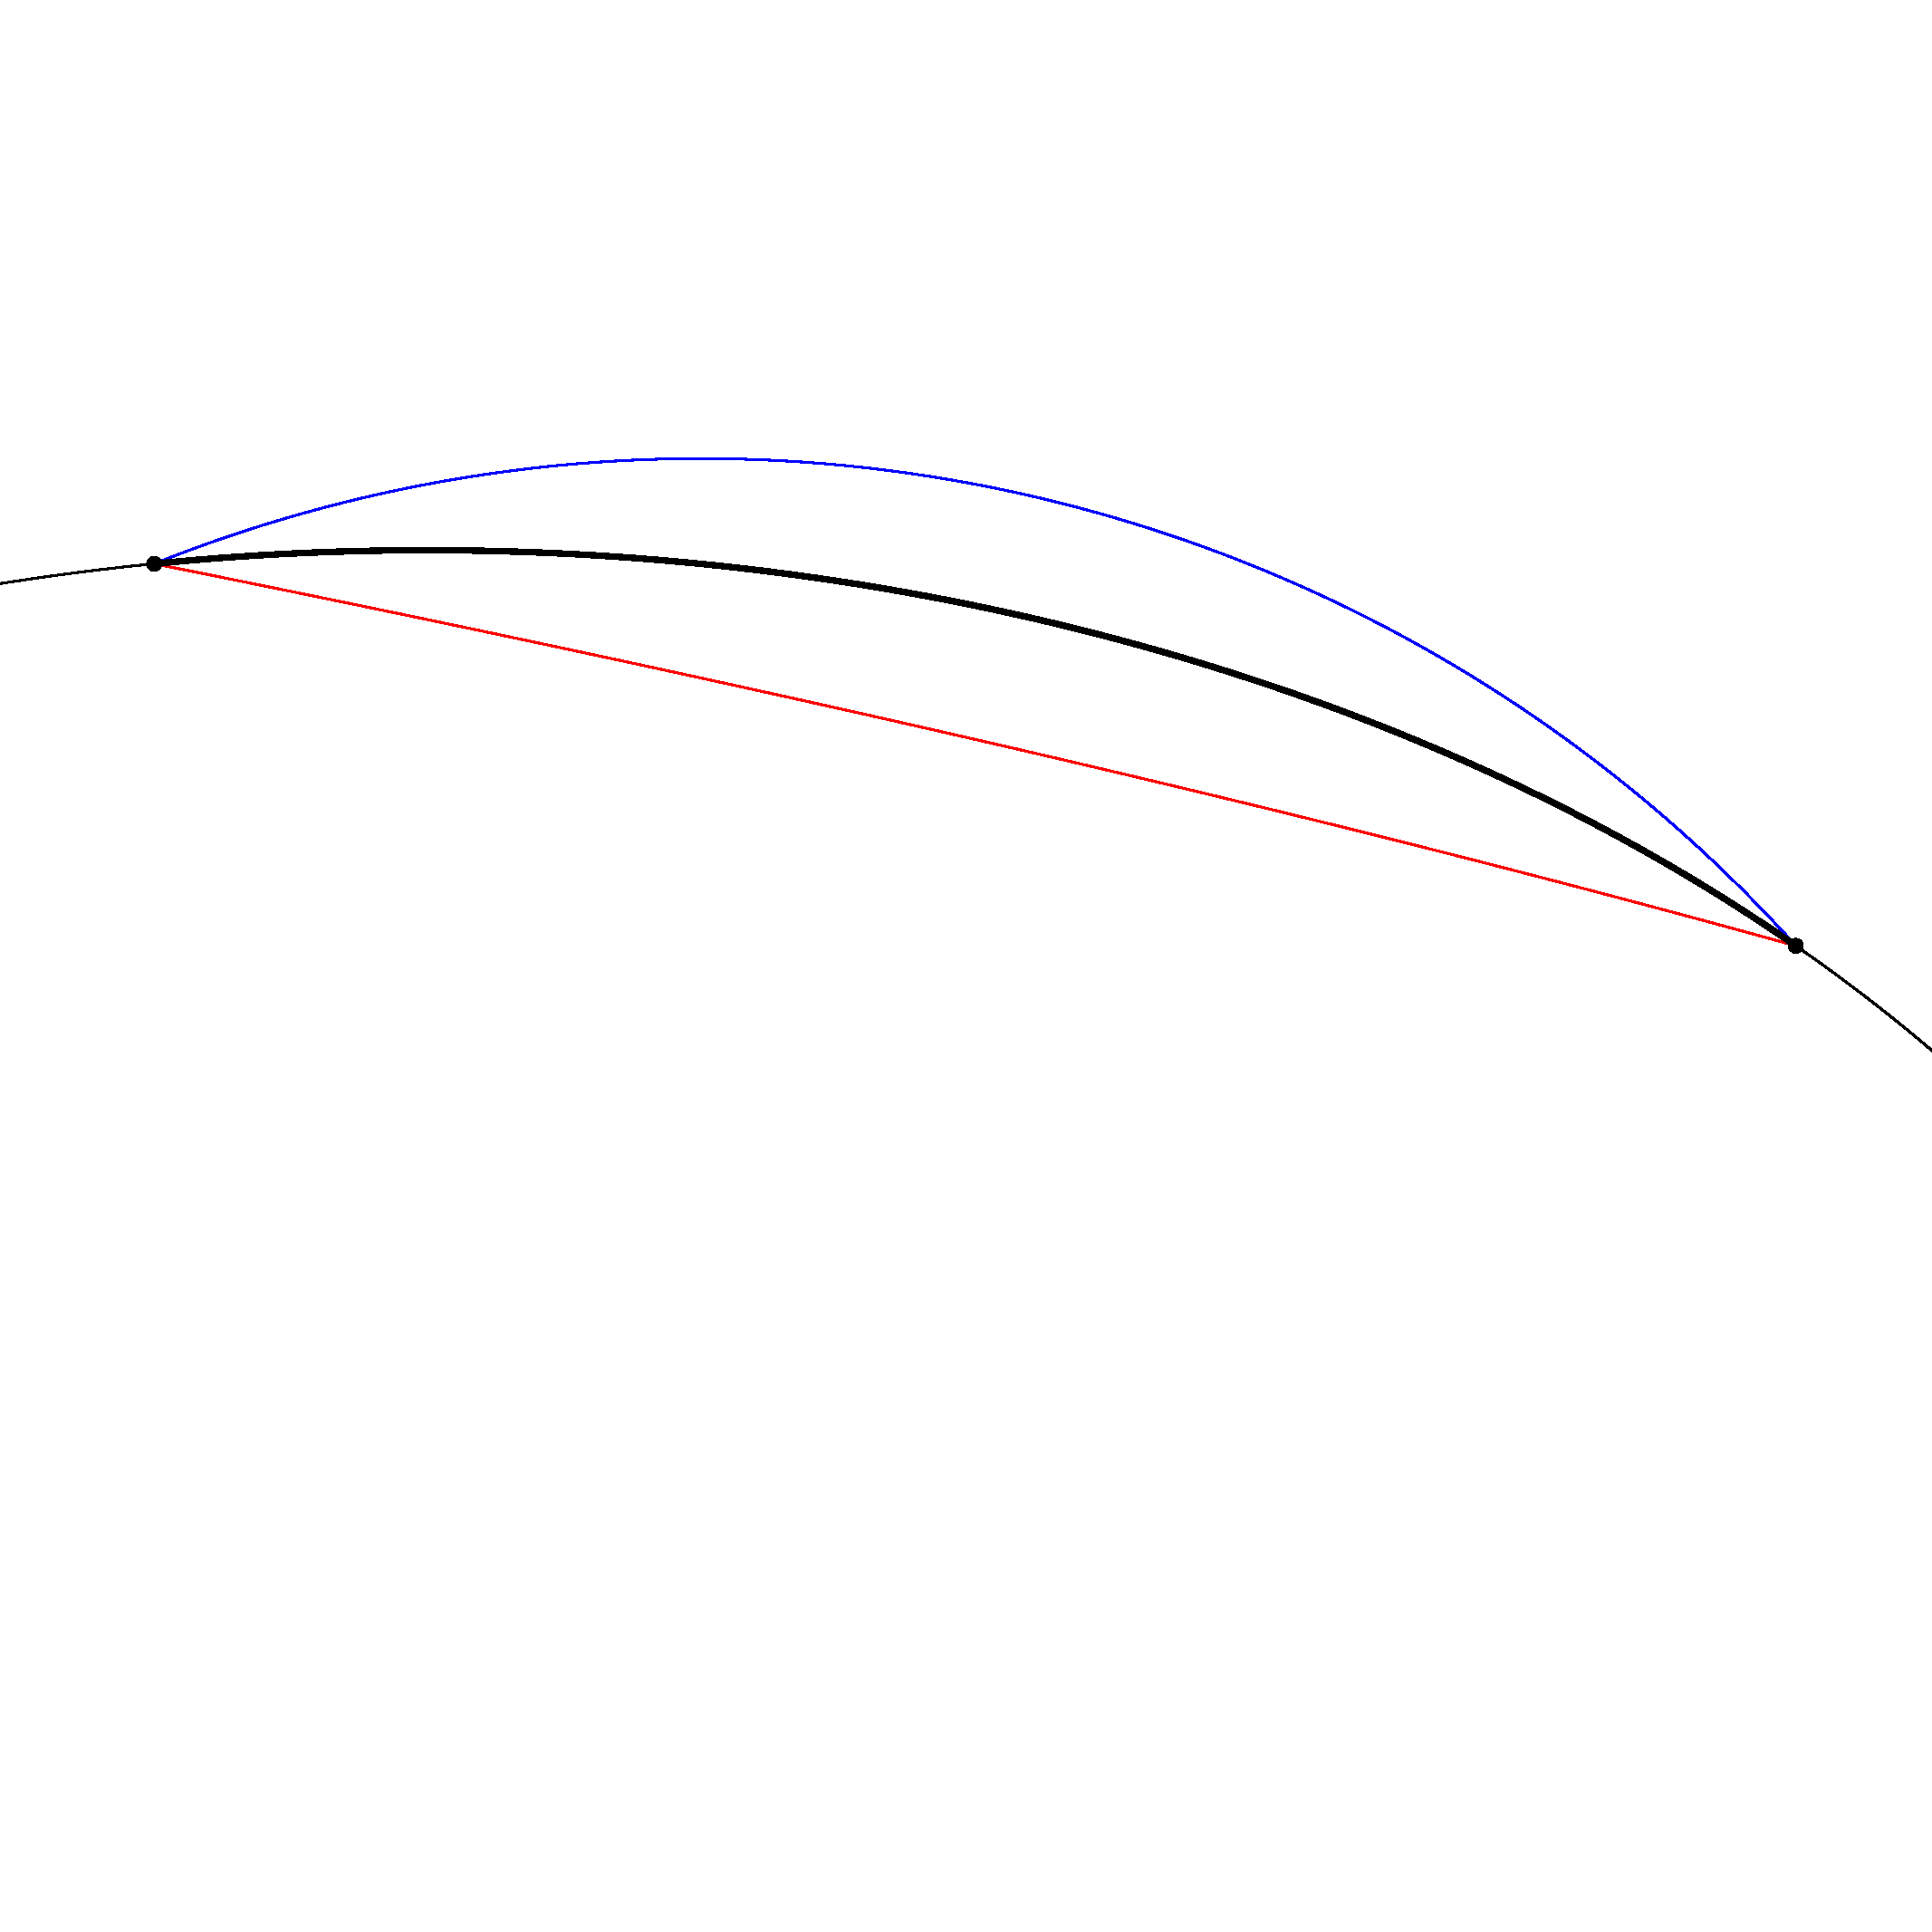
\includegraphics[width=0.3\textwidth]{EMgeodesicFR1D-1.pdf} &
%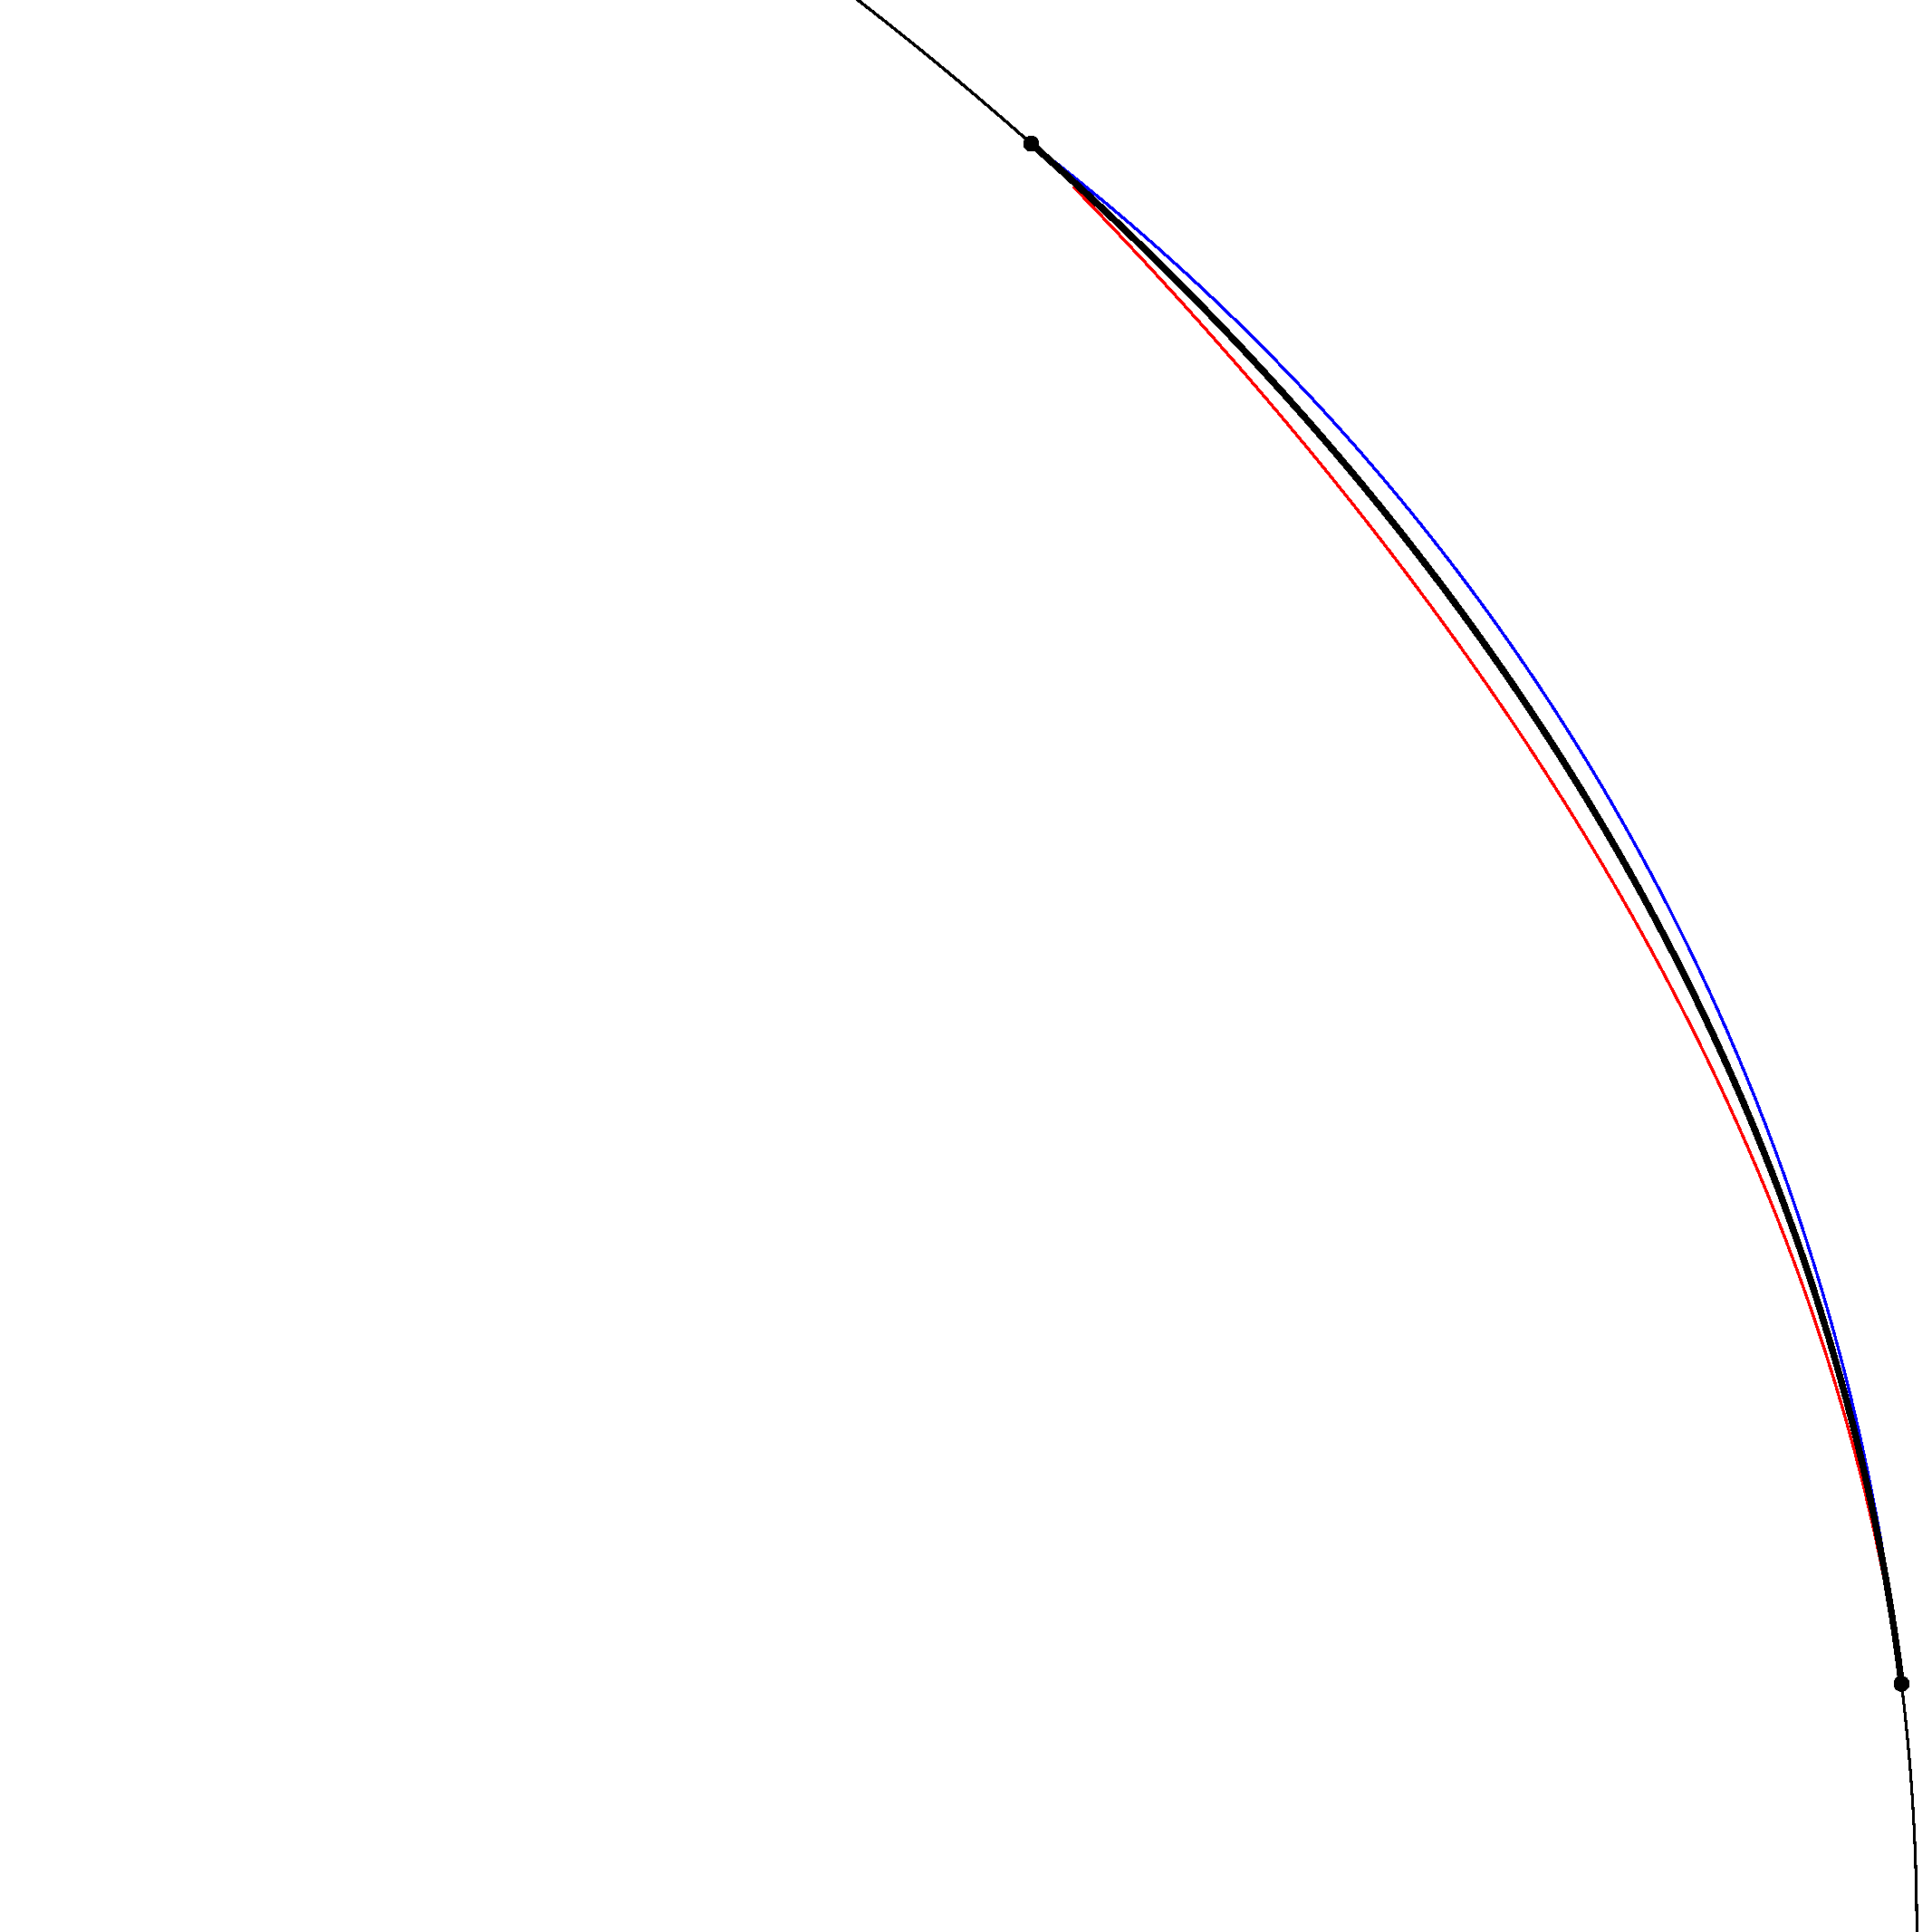
\includegraphics[width=0.3\textwidth]{EMgeodesicFR1D-2.pdf}
%\end{tabular}
%\caption{The full Fisher–Rao geodesic is shown in gray with the geodesic arc linking two univariate normal distributions shown in black. The exponential geodesics are shown in red and are below the Fisher–Rao geodesic. The mixture geodesics are shown in blue and are above the Fisher–Rao geodesic.}\label{fig:emgeodesic1d}
%\end{figure}

 
First, we draw multivariate normals by sampling means $\mu\sim\mathrm{Unif}(0,1)$ and sample covariance matrices $\Sigma$ as follows: We draw a lower triangular matrix $L$ with entries $L_{ij}$ iid sampled from $\mathrm{Unif}(0,1)$, and~take $\Sigma=LL^\top$.
We use $T=1000$ samples on curves and repeat the experiment $1000$ times
to gather average statistics on $\kappa_c$'s of curves. Results are summarized in Table~\ref{tab1}.
 

\begin{table}[H]
\caption{First set of experiments demonstrates the advantage of the $c_\CO(t)$ curve.\label{tab1}}
\setlength{\tabcolsep}{7mm}


\begin{tabular}{llllll}
\toprule
\boldmath{$d$} & \boldmath{$\kappa_\CO$} & \boldmath{$\kappa_l$} & \boldmath{$\kappa_e$} & \boldmath{$\kappa_m$} & \boldmath{$\kappa_{em}$} \\ \midrule
1	& {\bf {1.0025} %I confirm the bold is necessary. MDPI: Please confirm if the bold is unnecessary and can be removed. The following highlights are the same. Please confirm the bold in the whole text
}	& 	1.0414		& 1.1521		& 1.0236 & 1.0154\cr
2		& {\bf {1.0167}}	& 	1.0841	& 	1.1923		& 1.0631 & 1.0416\cr
3		& {\bf {1.0182}}		& 1.8997	& 	2.6072	& 	1.9965 & 1.07988\cr
4		& {\bf {1.0207}} 	& 	2.0793		& 1.8080	& 	2.1687 & 1.1873\cr
5		& {\bf {1.0324}}	& 	4.1207	& 	12.3804	& 	5.6170 & 4.2349\cr
\bottomrule
\end{tabular}

\end{table}

 


For that scenario that the C\&O curve (either $\bar c_\CO\in\barN$ or $c_\CO\in\calN$) performs best compared to the linear interpolation curves with respect to source parameter ($l$), mixture geodesic ($m$),   exponential geodesic ($e$), or~exponential-mixture mid-curve ($\mathrm{em}$).
Let us point out that we sample $\gamma_\calP(\barP_1,\barP_2;\frac{i}{T})$ for $i\in\{0,\ldots, T\}$.


Strapasson, Porto, and Costa~\cite{strapasson2015bounds}  (SPC)reported the following upper bound on the Fisher–Rao distance between multivariate normals 
$$\rho_\CO(N_1,N_2) \leq \rho_\calN(N_1,N_2) \leq U_\SPC(N_1,N_2),
$$ 
with:
\begin{equation}\label{prop:USPC}
 U_\SPC(N_1,N_2)=\sqrt{2\sum_{i=1}^d \log^2
\left( \frac{\sqrt{(1+D_{ii})^2+\mu_i^2} +\sqrt{(1-D_{ii})^2+\mu_i^2} }{\sqrt{(1+D_{ii})^2+\mu_i^2} -\sqrt{(1-D_{ii})^2+\mu_i^2}}\right)},
\end{equation}
where $\Sigma=\Sigma_1^{-\frac{1}{2}}\Sigma_2\Sigma_1^{-\frac{1}{2}}$, $\Sigma=\Omega D\Omega^\top$ is the eigen decomposition, and~$\mu=\Omega^\top \Sigma_1^{-\frac{1}{2}}(\mu_2-\mu_1)$. 
This upper bound performs better when the normals are well-separated and worse than the $\sqrt{D_J}$-upper bound when the normals are close to each other.

Let us compare $\rho_\CO(N_1,N_2)$ with $\rho_\calN(N_1,N_2) \approx \tilde\rho^{c_\CO}(N_1,N_2)$ and the upper bound $U(N_1,N_2)$ by averaging over $1000$ trials with $N_1$ and $N_2$ chosen randomly as before and $T=1000$. 
We have $\rho_\CO(N_1,N_2)\leq \rho_\calN(N_1,N_2) \approx \tilde\rho^{c_\CO}(N_1,N_2) \leq U(N_1,N_2)$.
Table~\ref{tab:comparebounds} shows that our Fisher–Rao approximation is close to the lower bound (and hence to the underlying true Fisher–Rao distance) and that the upper bound is about twice the lower bound for that particular scenario.
 
 
 \begin{table}[H]
\caption{Comparing our Fisher–Rao approximation with the Calvo and Oller lower bound and the 
 upper~bound of~\cite{strapasson2015bounds}.\label{tab:comparebounds}}
\setlength{\tabcolsep}{10mm}
\begin{tabular}{llll}
\toprule
\boldmath{$d$} & \boldmath{$\rho_\CO(N_1,N_2)$} & \boldmath{$\tilde\rho^{c_\CO}(N_1,N_2)$} & \boldmath{$U(N_1,N_2)$} \\ \hline
1 & 1.7563 & 1.8020 & 3.1654 \cr
2 & 3.2213 & 3.3194 & 6.012 \cr
3 & 4.6022 & 4.7642 & 8.7204 \cr
4 & 5.9517 & 6.1927 & 11.3990 \cr
5 & 7.156 & 7.3866 & 13.8774 \cr
\bottomrule
\end{tabular}
\end{table}


 
 
% \end{paracol}\end{document}


 





 
 






%Figure~\ref{fig:vizgeo1d} displays some geodesics on the Fisher–Rao univariate normal manifold.
%Figure~\ref{fig:viz1d} displays the considered geodesics and curves in  the stretched Poincar\'e upper plane of univariate normal distributions ($x$-axis is stretched by $\sqrt{2}$) (in 1D for illustration purpose).

%\begin{figure}
%\centering
%\begin{tabular}{ccc}
%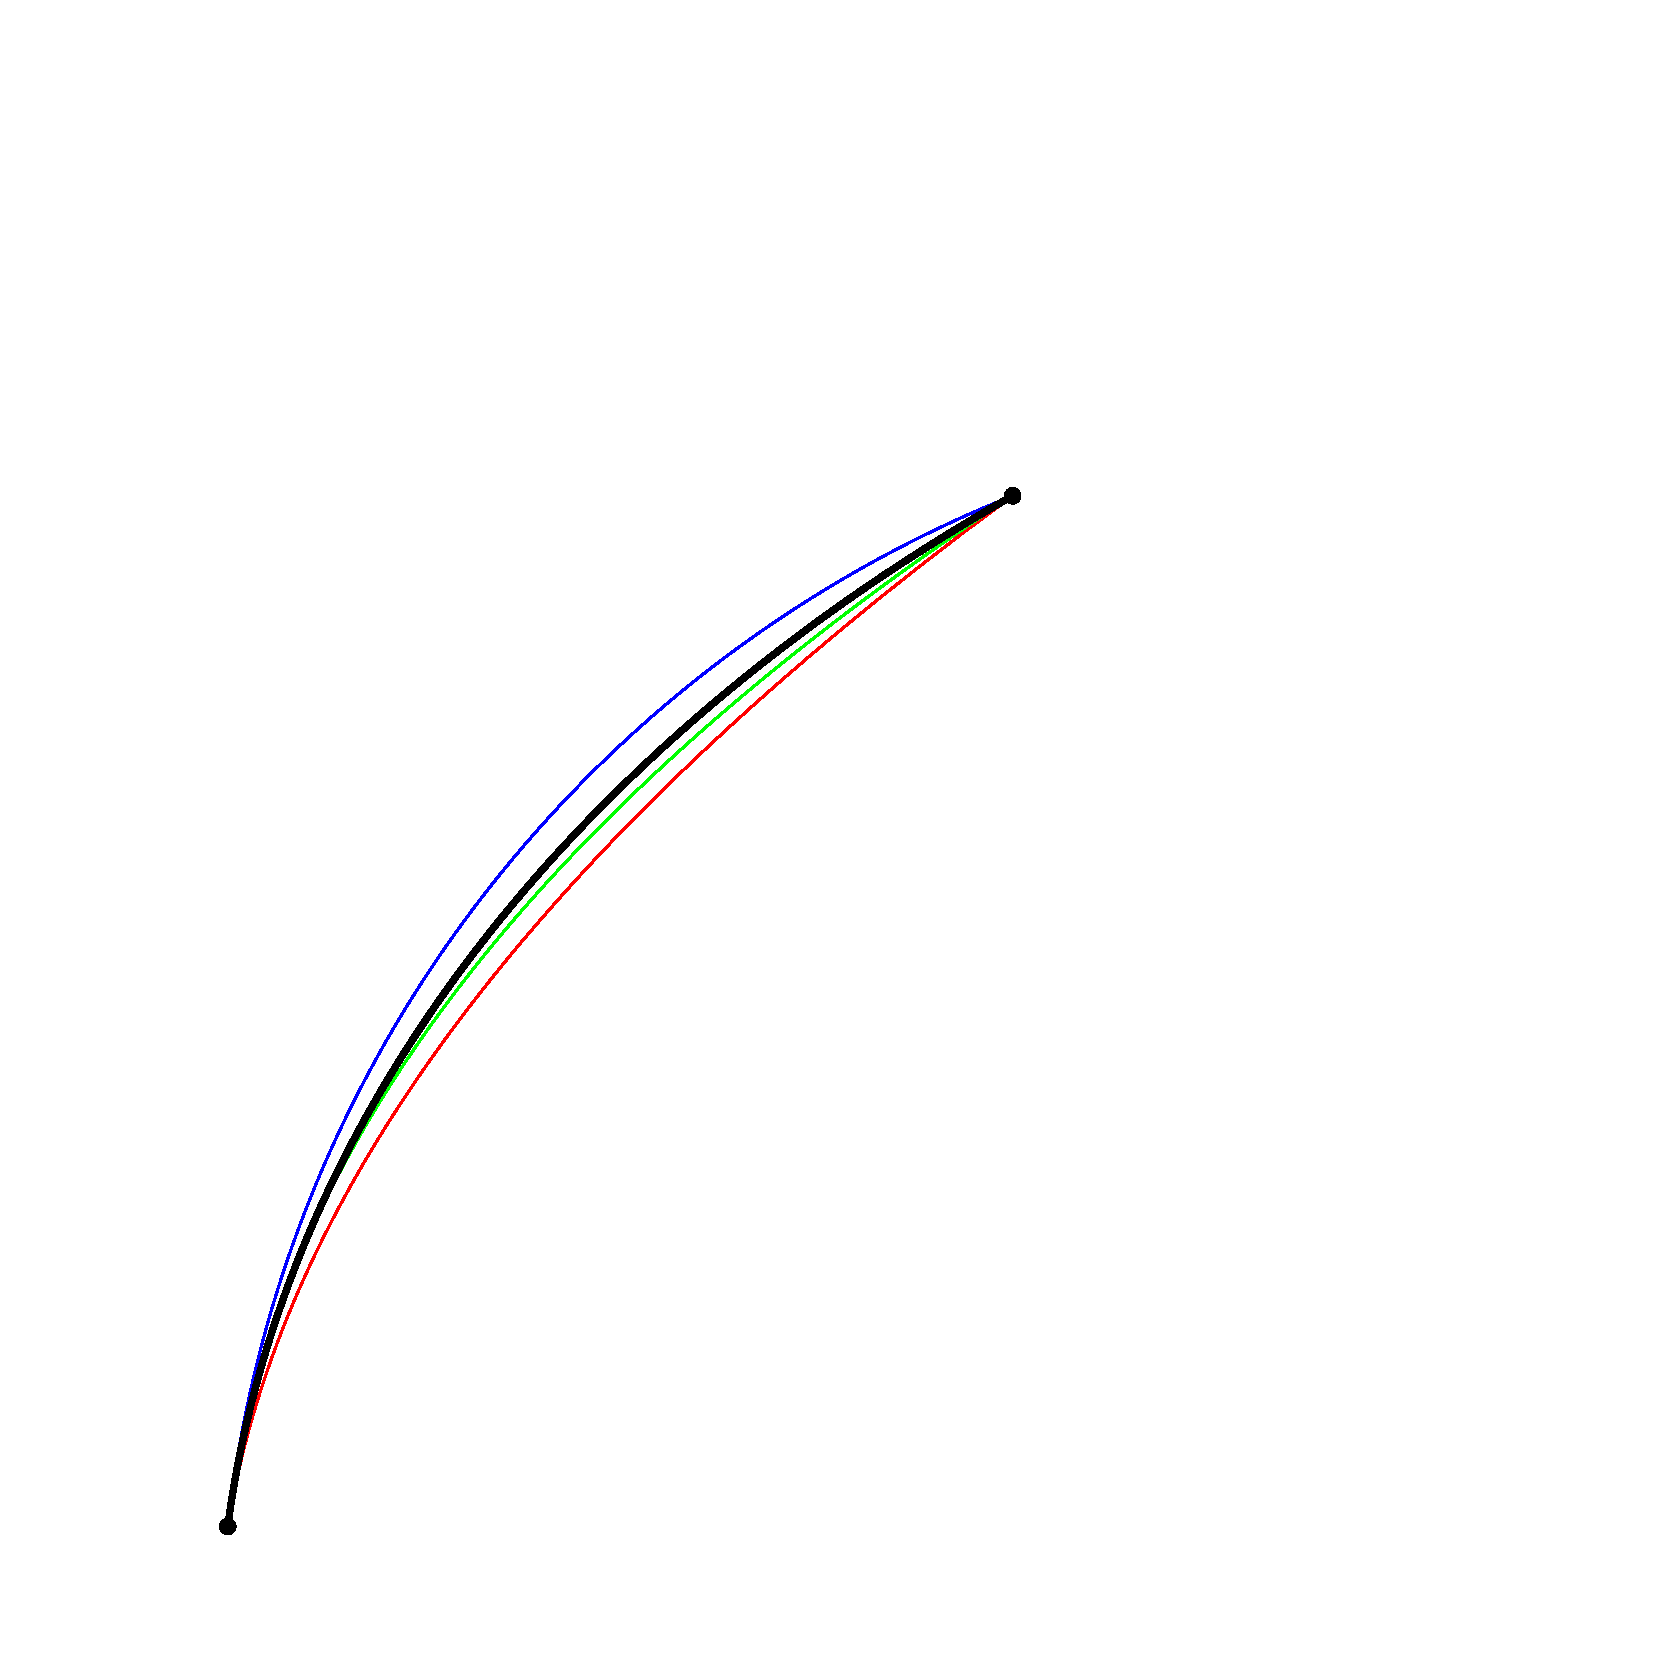
\includegraphics[width=0.3\textwidth]{T1.pdf} &
%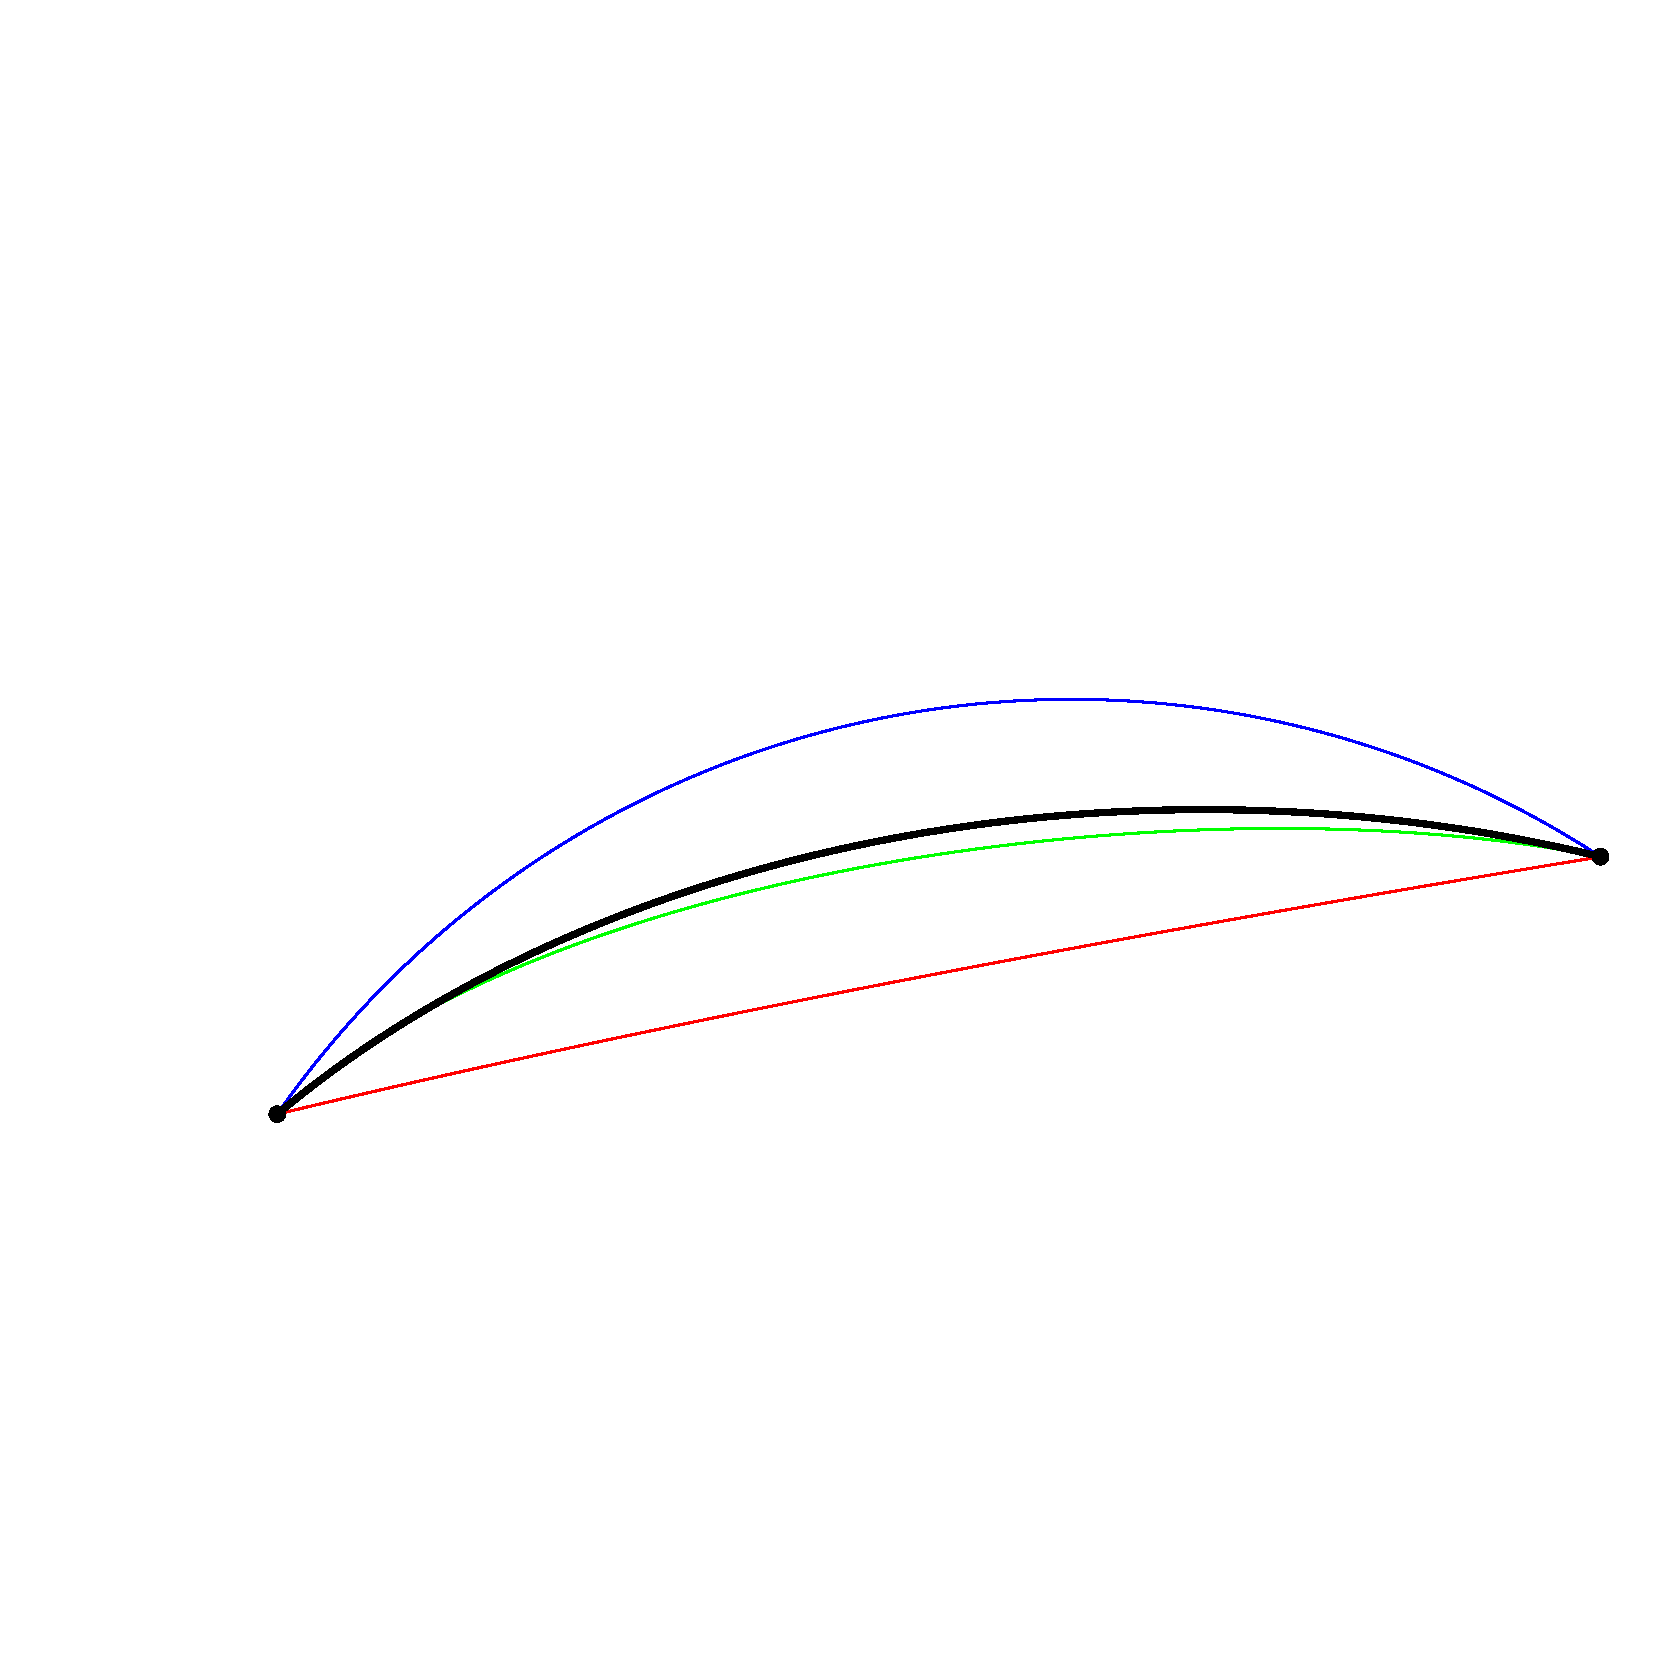
\includegraphics[width=0.3\textwidth]{T2.pdf}&
%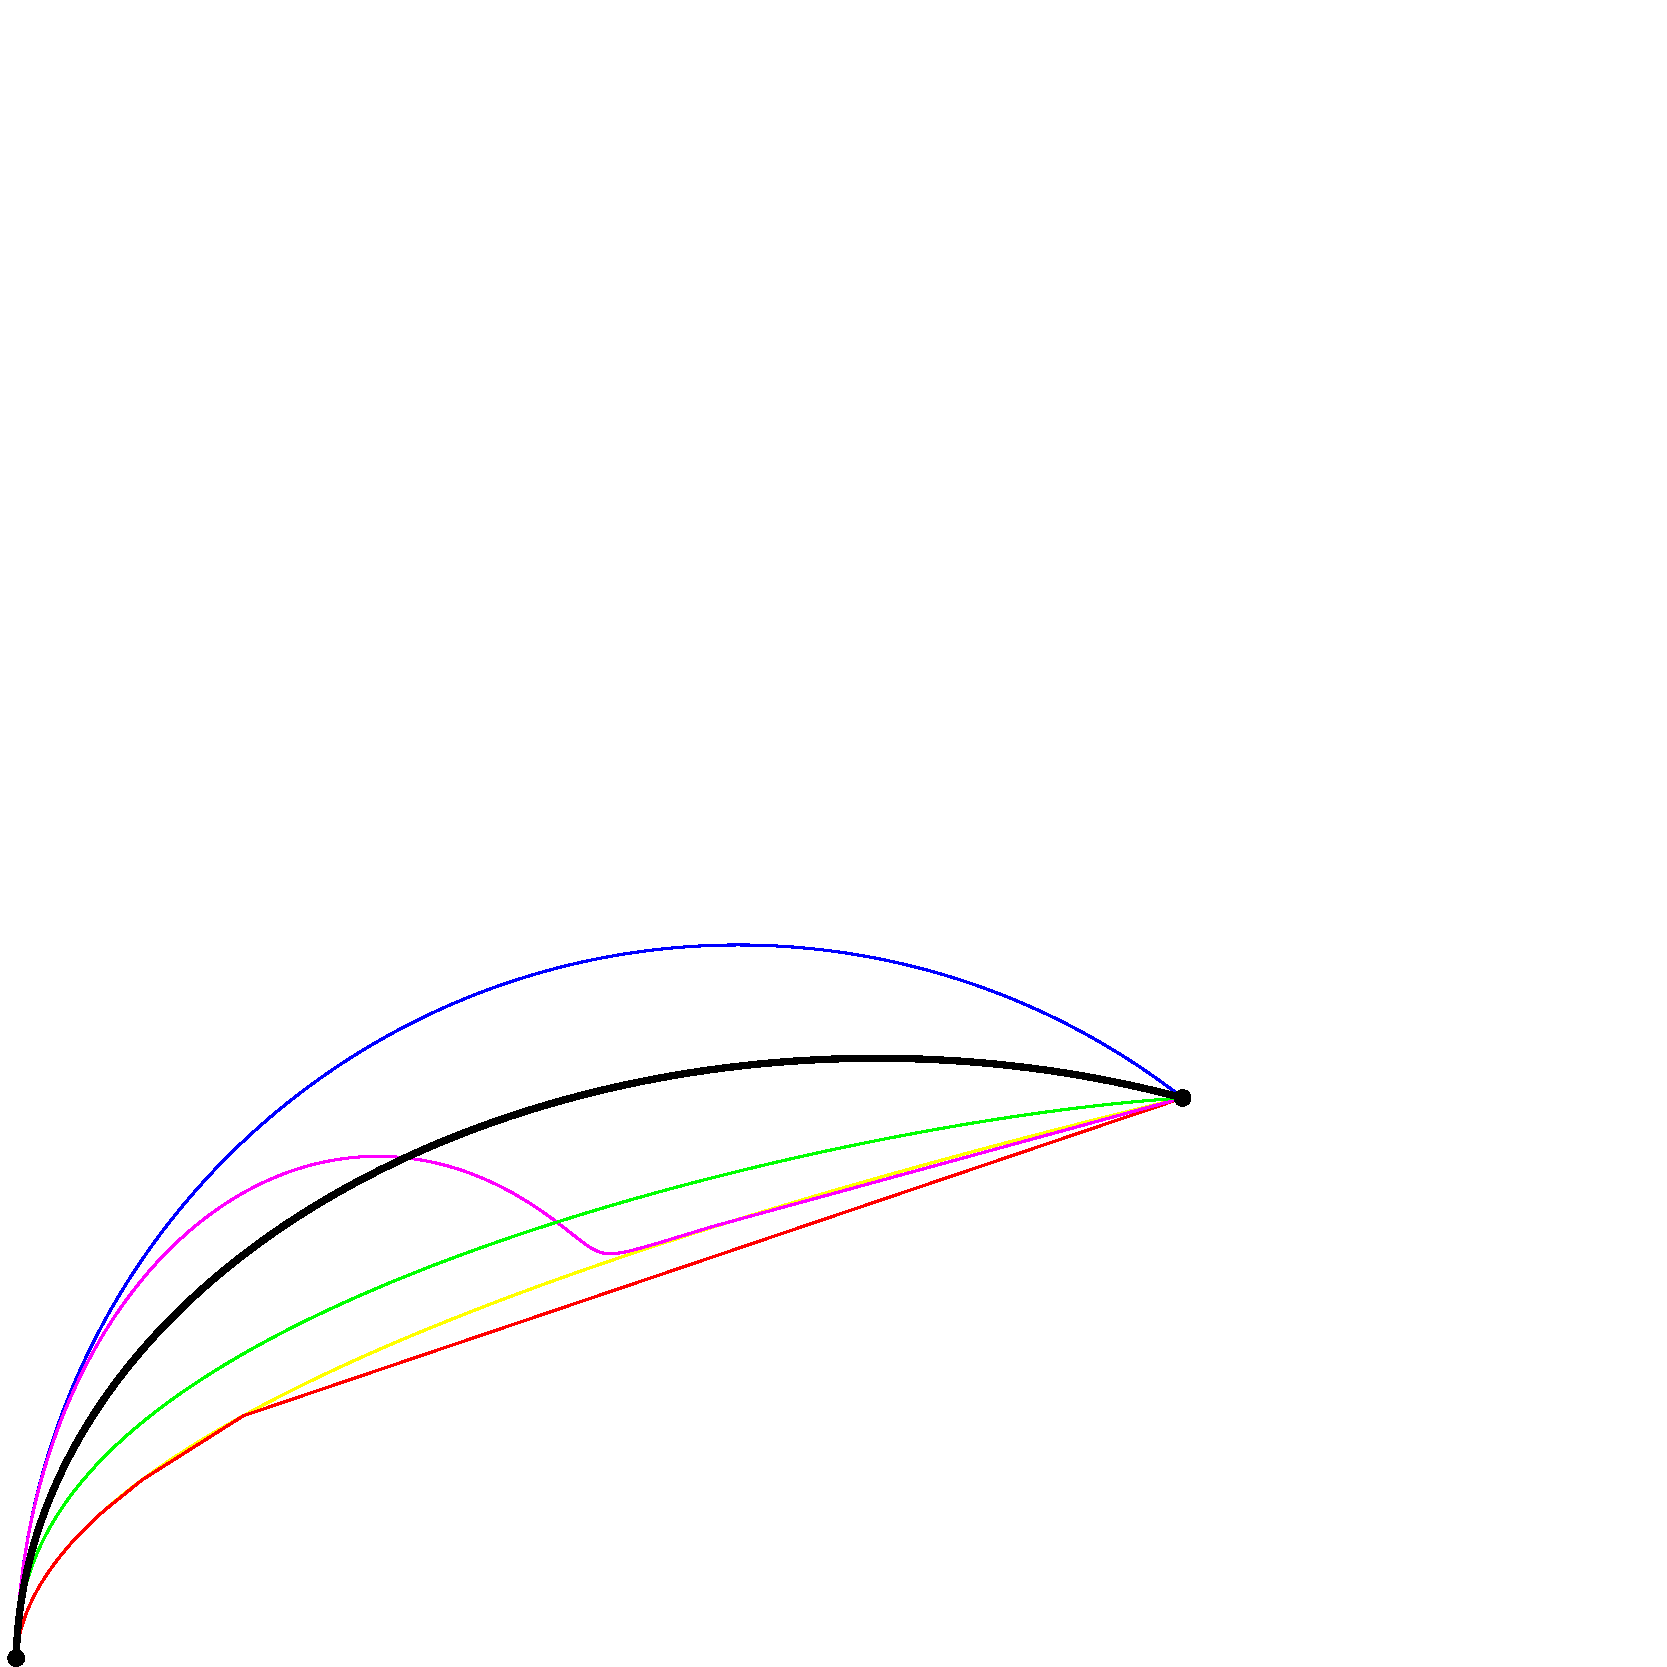
\includegraphics[width=0.3\textwidth]{T3.pdf} 
%\end{tabular}
%%
%\caption{Visualizing the geodesics and curves in the Poincar\'e upper plane with $x$-axis stretched by $\sqrt{2}$: 
%(a) and (b): Fisher–Rao geodesic (black), our projected Calvo \& Oller curve (green), the mixture geodesic (blue), and the exponential geodesic (red). (c): interpolation in ordinary parameterization $\lambda$ (yellow), mid-mixture-exponential curve (purple). The range is $[-1,1]\times (0,2]$.
 %\label{fig:viz1d}}
%\end{figure}



Second, since the distances are invariant under the action of the affine group, we can set wlog. $N_1=(0,I)$ (standard normal distribution) and let $N_2=\diag(u_1,\ldots, u_d)$ where $u_i\sim\mathrm{Unif}(0,a)$. As~normals $N_1$ and $N_2$ separate from each other, we notice experimentally that the performance of the $c_\CO$ curve degrades in the second experiment with $a=5$  (see Table~\ref{tab2}):
Indeed, the~mixture geodesic works experimentally better than the C\&O curve when $d\geq 11$.

\begin{table}[H]
\caption{Second set of experiments shows limitations of the $c_\CO(t)$ curve.}\label{tab2}
\setlength{\tabcolsep}{9.6mm}
\begin{tabular}{lllll}
\toprule
\boldmath{$d$} & \boldmath{$\kappa_\CO$} & \boldmath{$\kappa_l$} & \boldmath{$\kappa_e$} & \boldmath{$\kappa_m$} \\ \midrule
1		&   {\bf {1.0569}}	& 	1.1405	& 1.139		& 1.0734\cr
5	 	&  {\bf {1.1599}}		& 1.4696		& 1.5201		& 1.1819\cr
10	& 	{\bf {1.2180}}	& 	1.6963	& 	1.7887		& 1.2184\cr
11		& 1.2260	& 	1.7333	& 	1.8285	& 	{\bf {1.2235}}\cr
12		& 1.2301	& 1.7568		& 1.8539		& {\bf {1.2282}}\cr
15		& 1.2484	& 	1.8403		& 1.9557		& {\bf {1.2367}} \cr
20		& 1.2707		& 1.9519	& 	2.0851	& 	{\bf {1.2466}}\cr
\bottomrule
\end{tabular}

\end{table}


Figure~\ref{fig:viz2Dbis} display the various curves considered for approximating the Fisher–Rao distance between bivariate normal distributions: For a curve $c(t)$, we visualize its corresponding bivariate normal distributions $(\mu_{c(t)},\Sigma_{c(t)})$ at several increment steps $t\in [0,1]$ by plotting the ellipsoid 
$$
E_{c(t)}=\mu_{c(t)}+\left\{L^\top x, x=(\cos\theta,\sin\theta), \theta\in [0,2\pi)\right\},
$$
where $\Sigma_{c(t)}=L_{c(t)}L^\top_{c(t)}$.


%\begin{figure}
%\centering
%\begin{tabular}{ccc}
%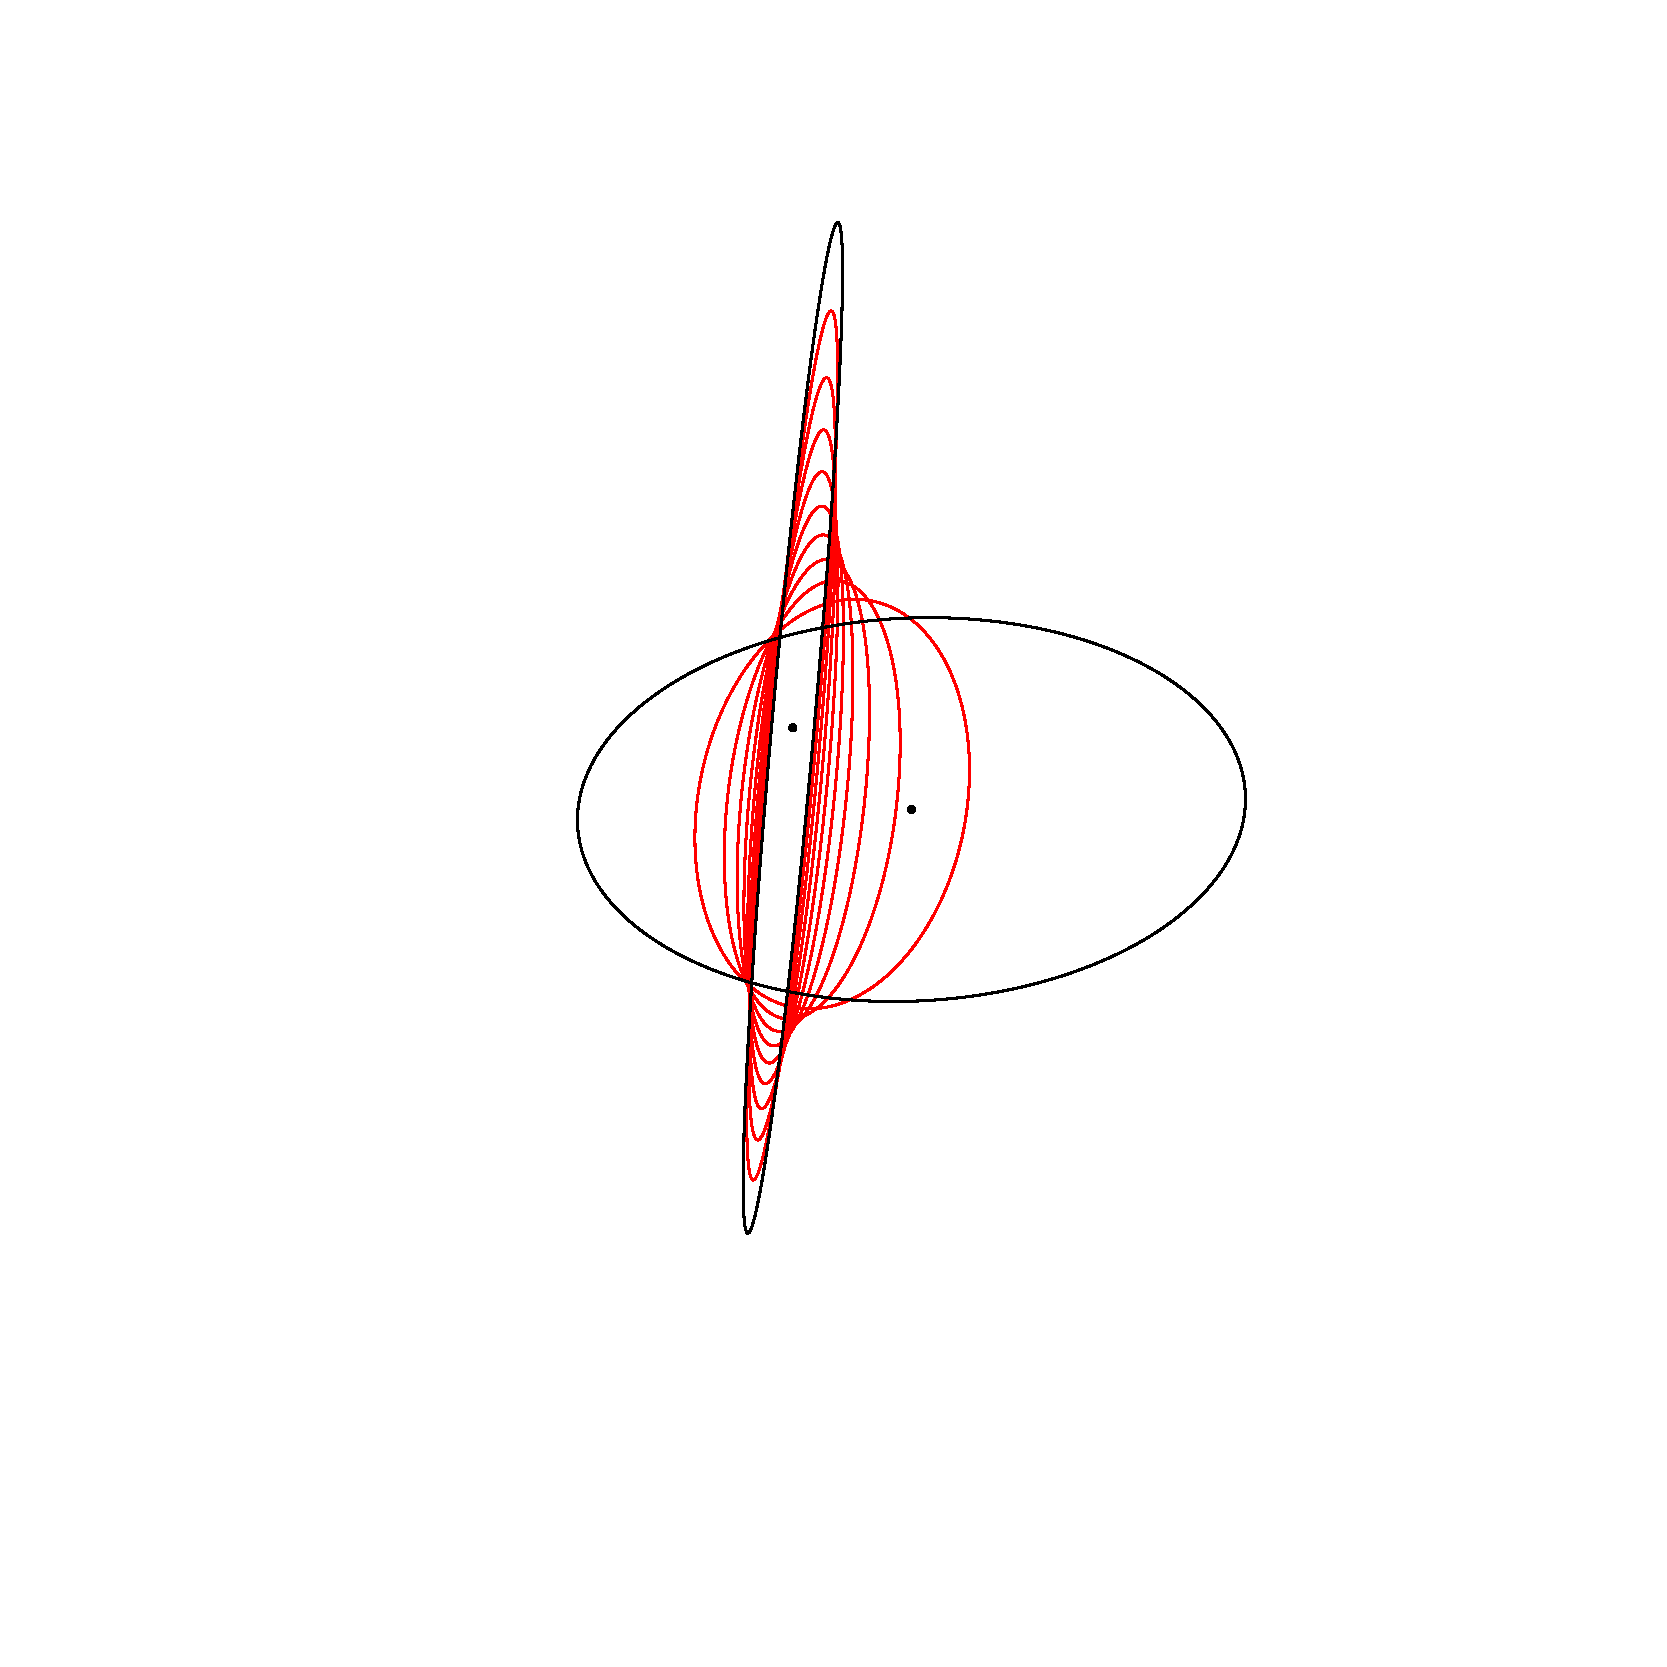
\includegraphics[width=0.3\textwidth]{BivariateNormal-T.pdf} &
%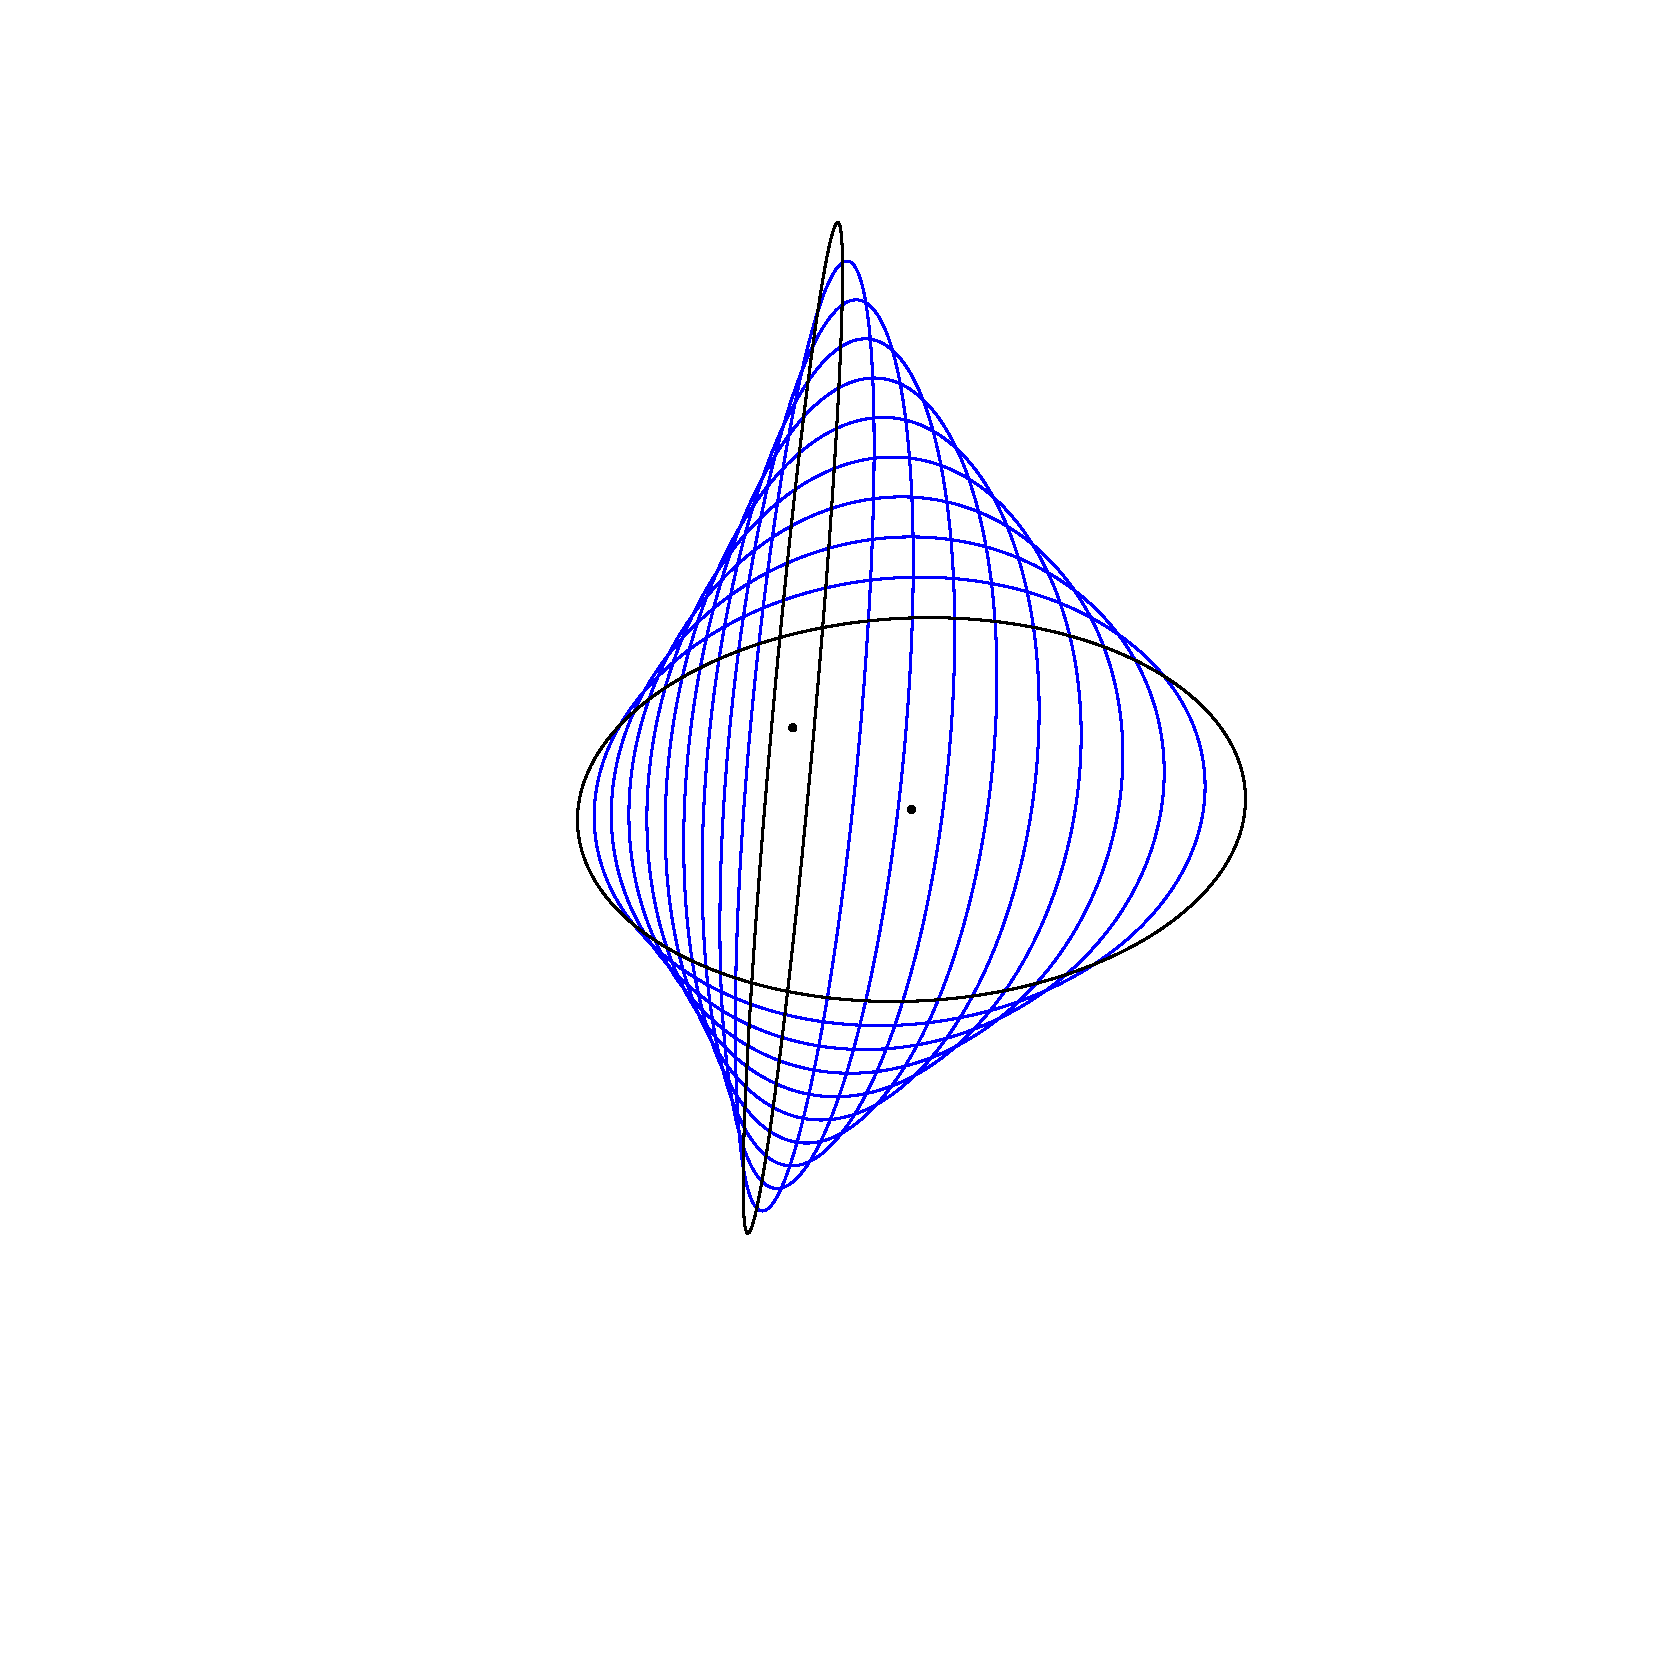
\includegraphics[width=0.3\textwidth]{BivariateNormal-E.pdf}&
%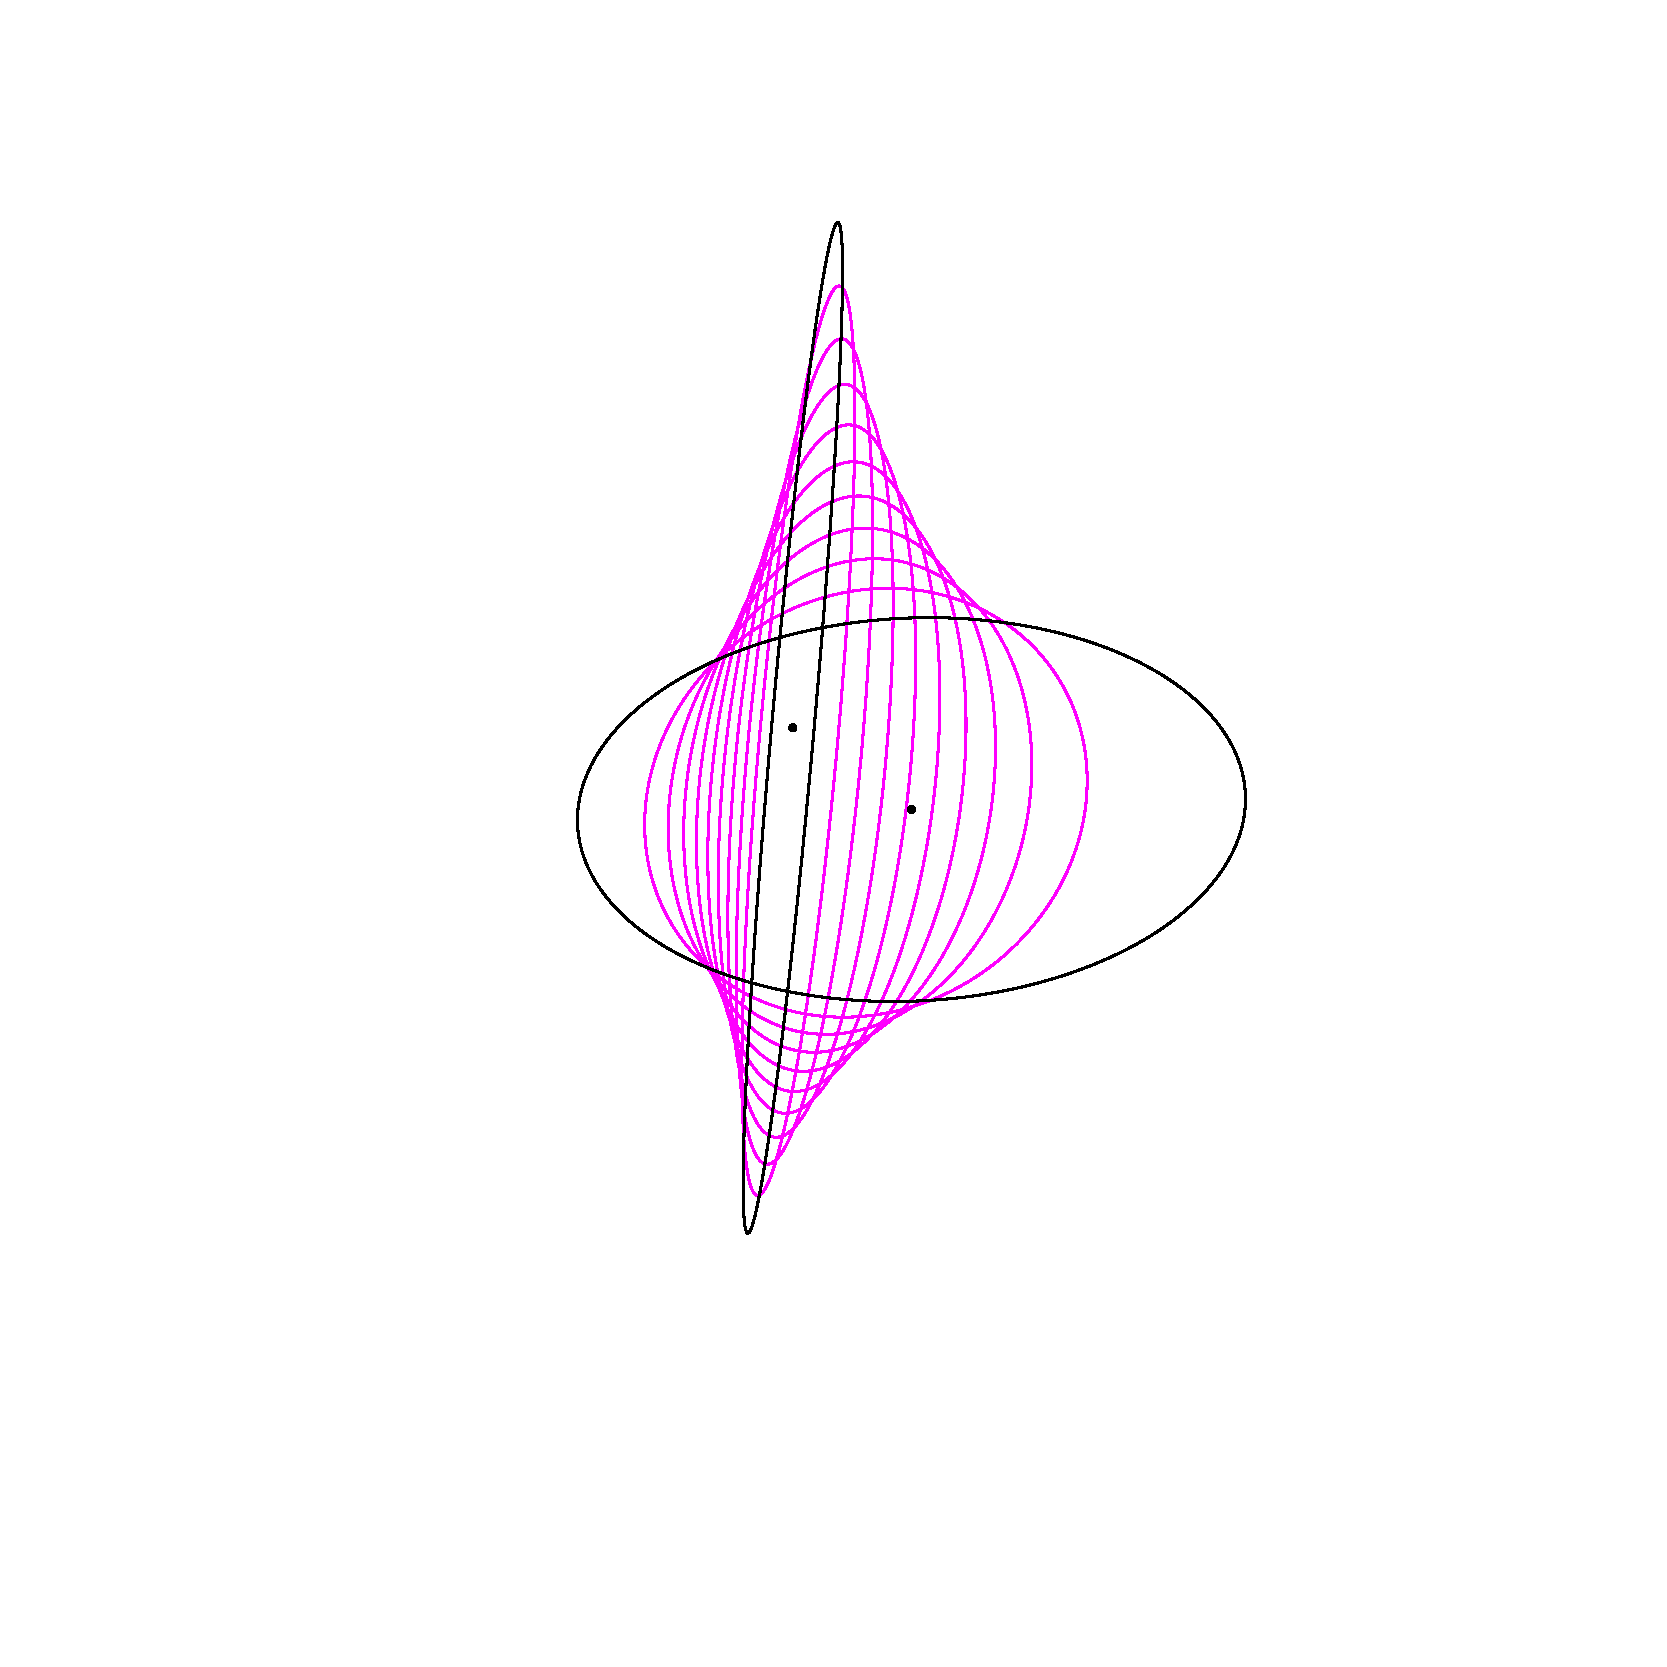
\includegraphics[width=0.3\textwidth]{BivariateNormal-ET.pdf} \\
%(a) & (b) & (c)\cr
%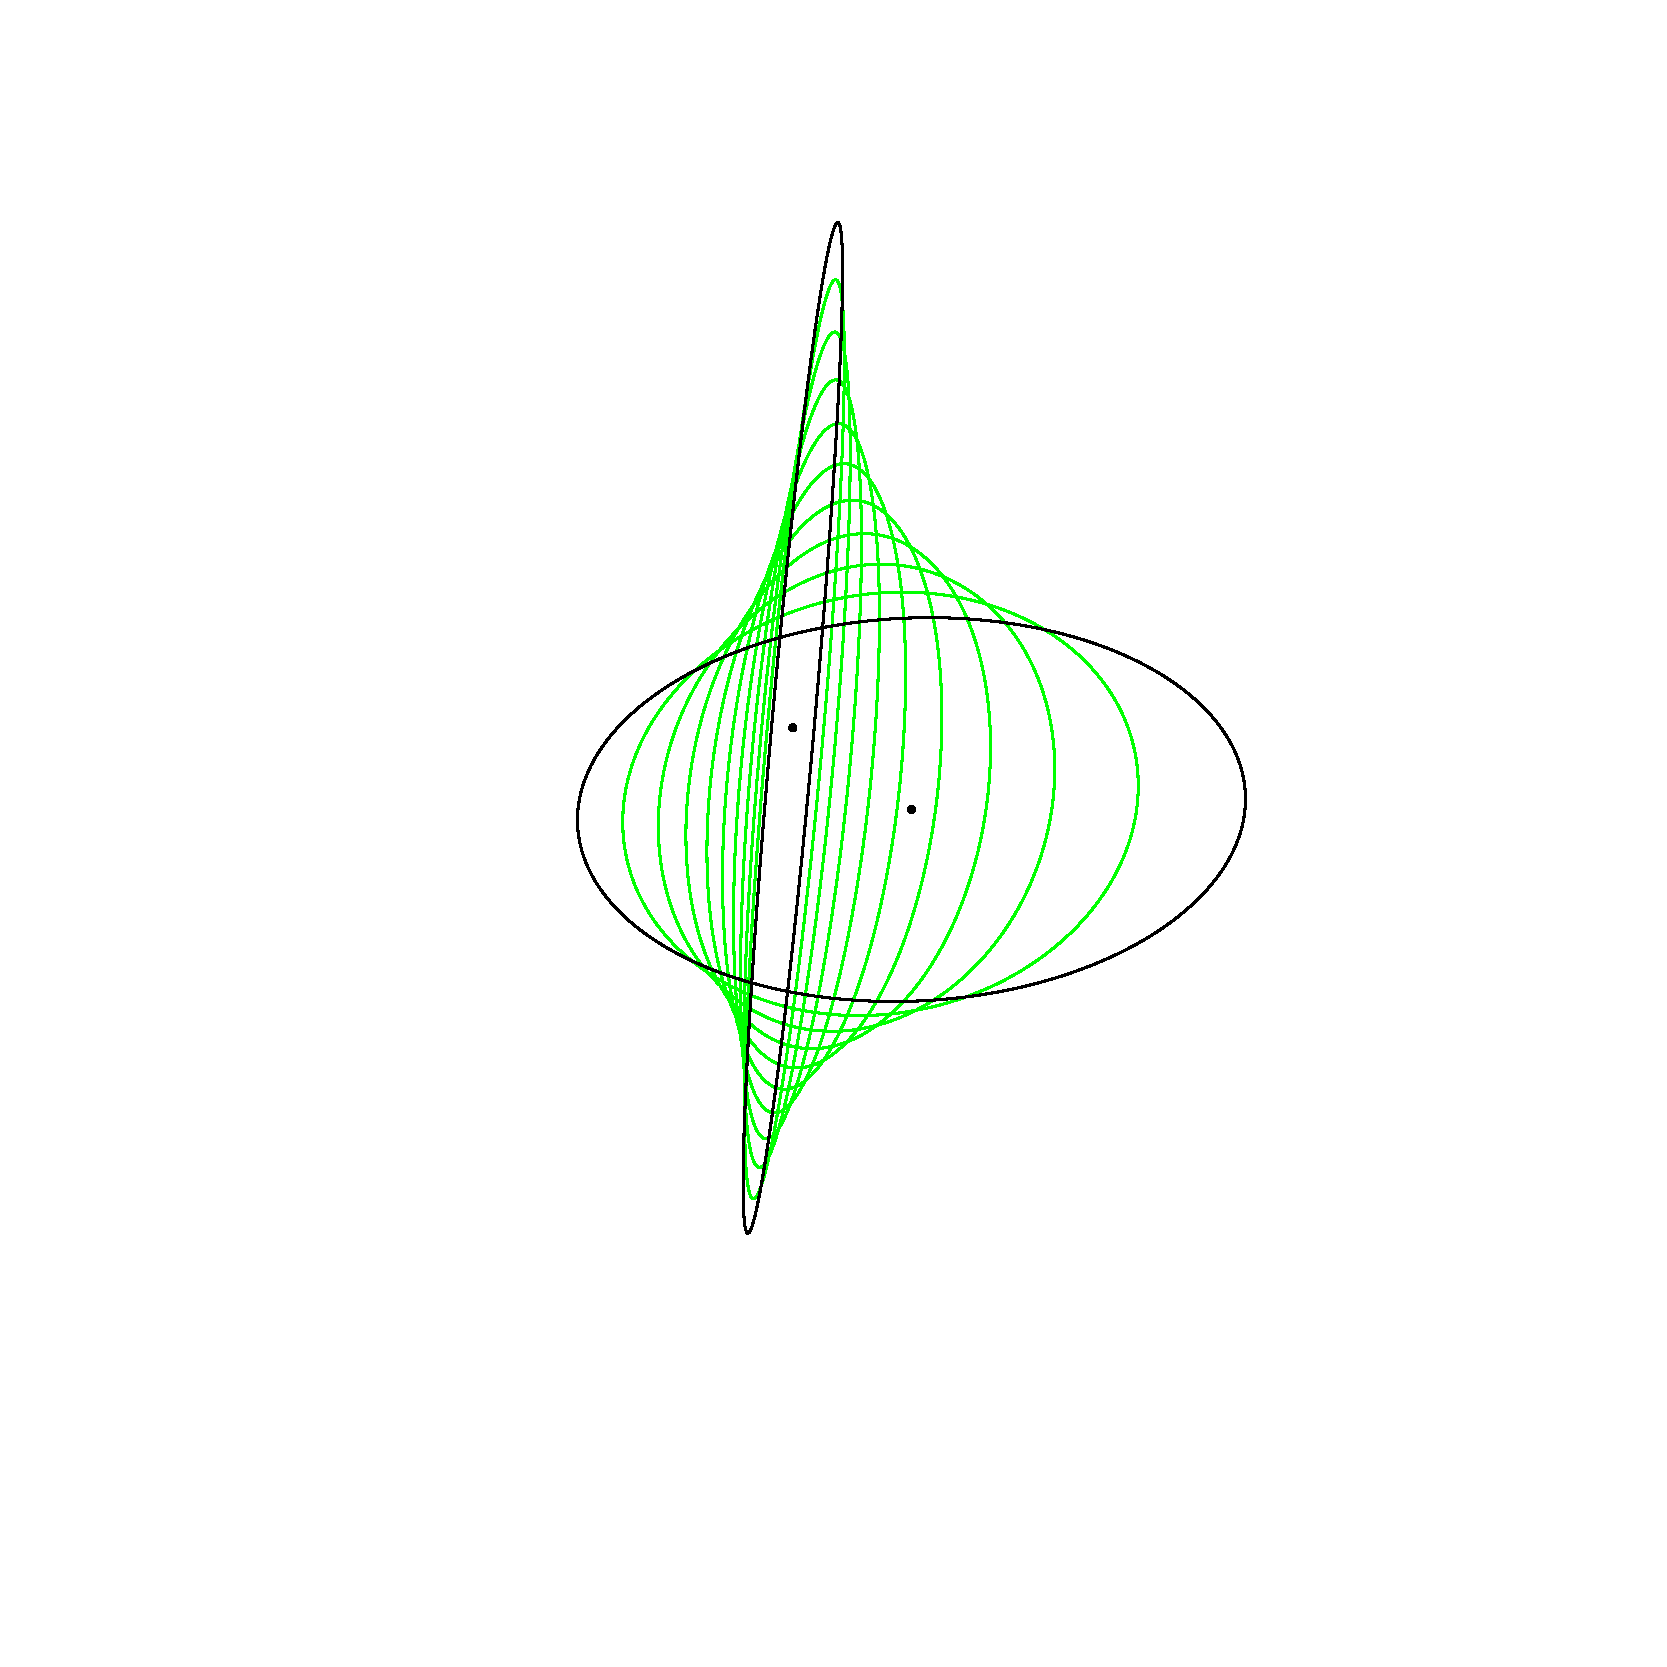
\includegraphics[width=0.3\textwidth]{BivariateNormal-CO.pdf} &
%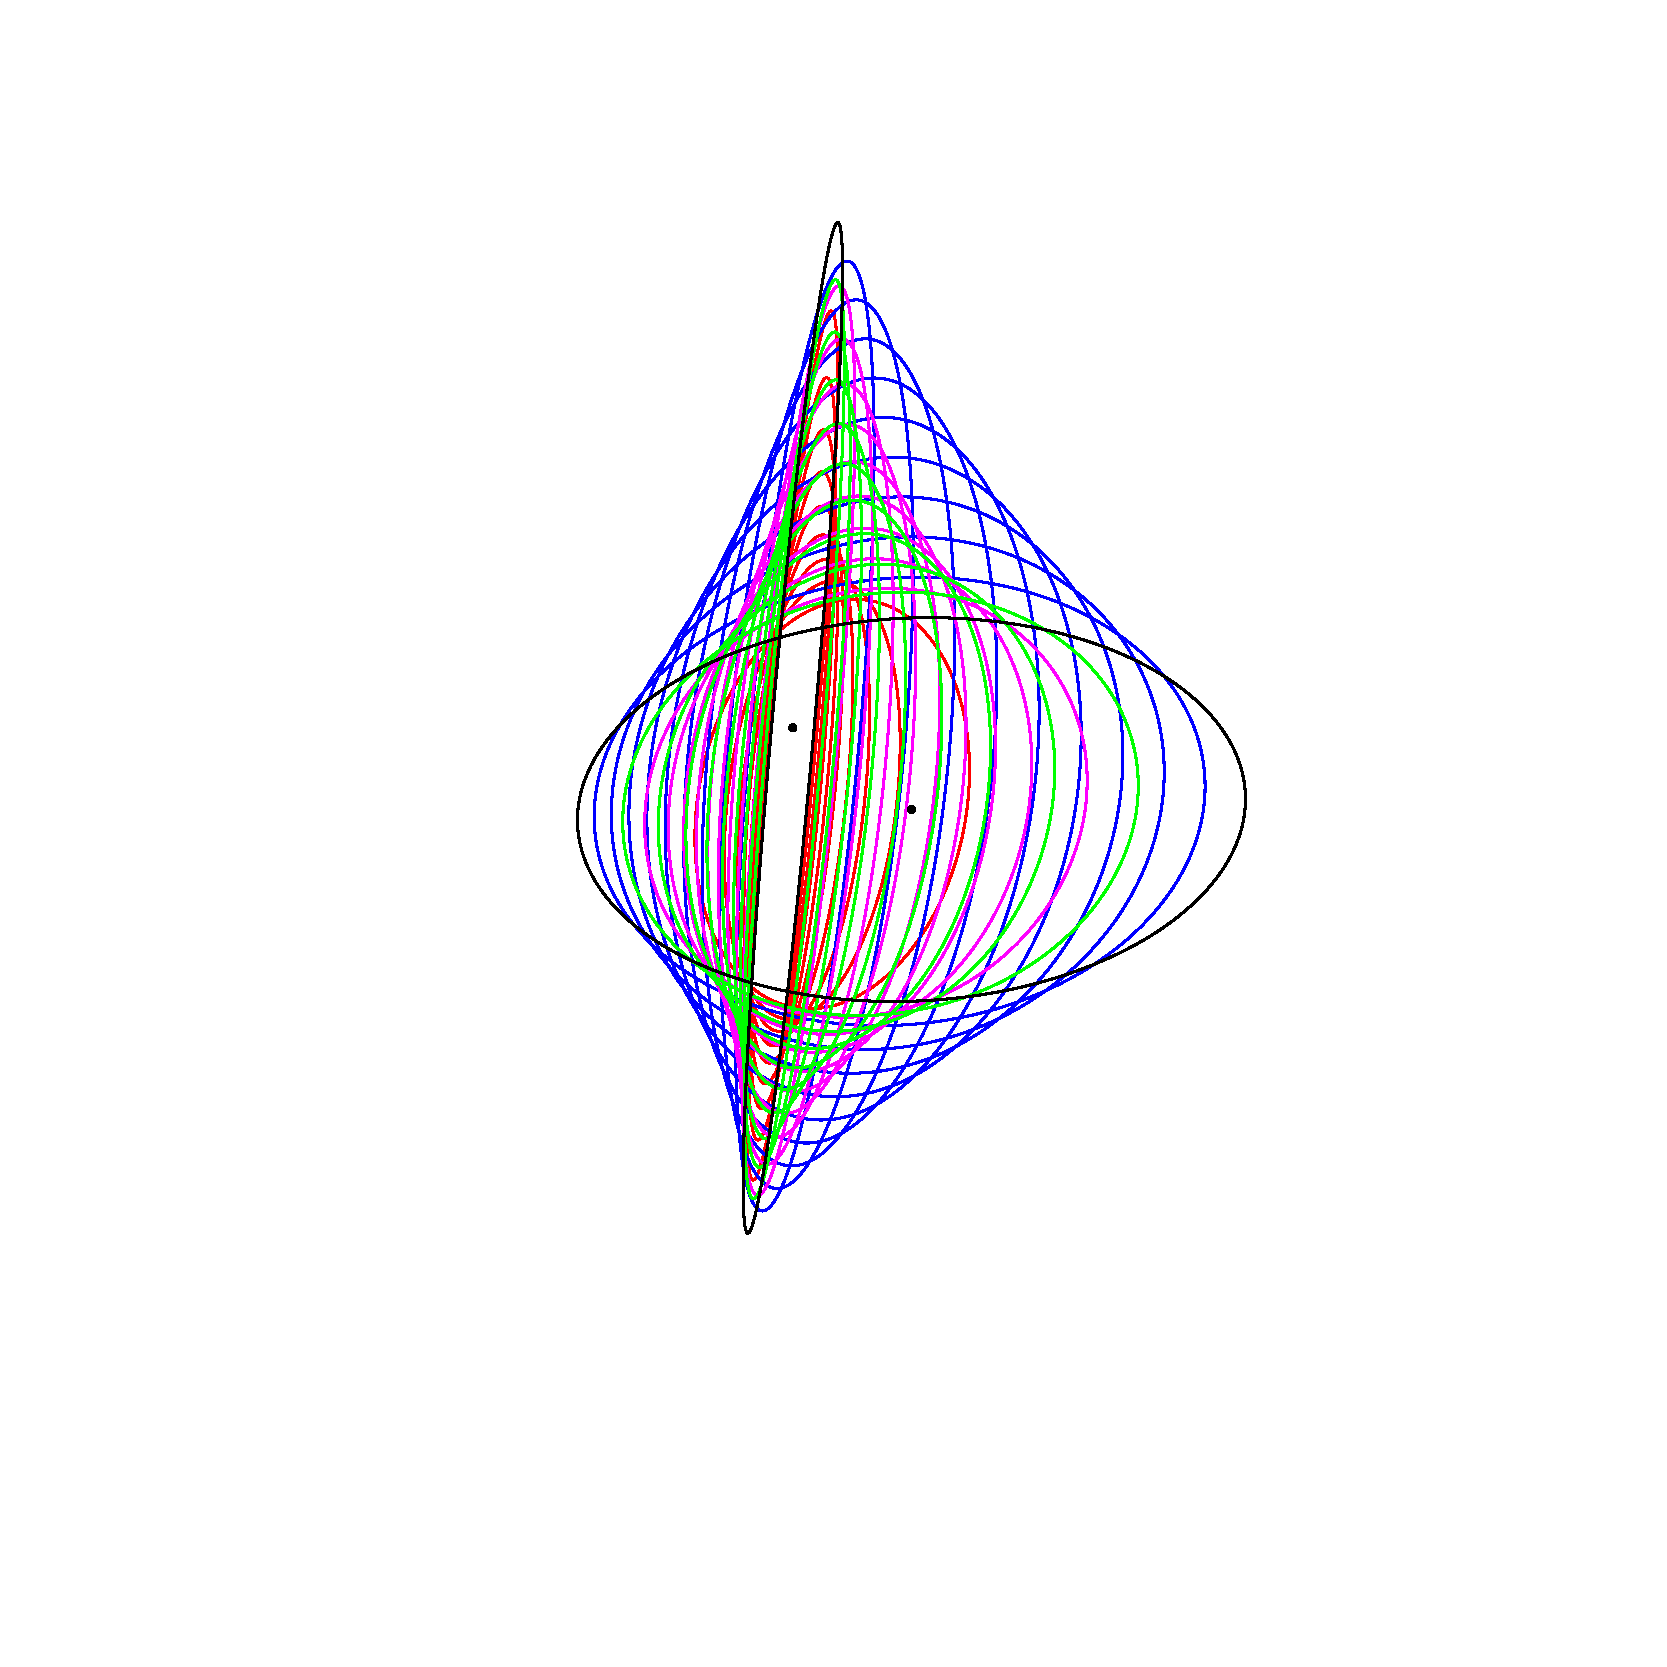
\includegraphics[width=0.3\textwidth]{BivariateNormalAll.pdf}& \\
%(d) &(e)
%\end{tabular}
%%
%\caption{Visualizing at discrete positions (10 increment steps between $0$ and $1$) some curves used to approximate the Fisher–Rao distance between two bivariate normal distributions:
%(a) exponential geodesic $c^e=\gamma_\calN^e$ (red),
%(b) mixture geodesic $c^m=\gamma_\calN^m$ (blue),
%(c) mid mixture-exponential curve $c^{\mathrm{em}}$ (purple),
%(d) projected Calvo \& Oller curve $c^{\CO}$ (green), and
%(e) All superposed curves at once. 
%Visualization in the 2D sample space of bivariate normal distributions because bivariate normals are modeled as a $m=5$ dimensional point on the Fisher–Rao manifold $\calM$.
 %\label{fig:viz2D}}
%\end{figure}

\begin{figure}[H]

\begin{tabular}{ccc}
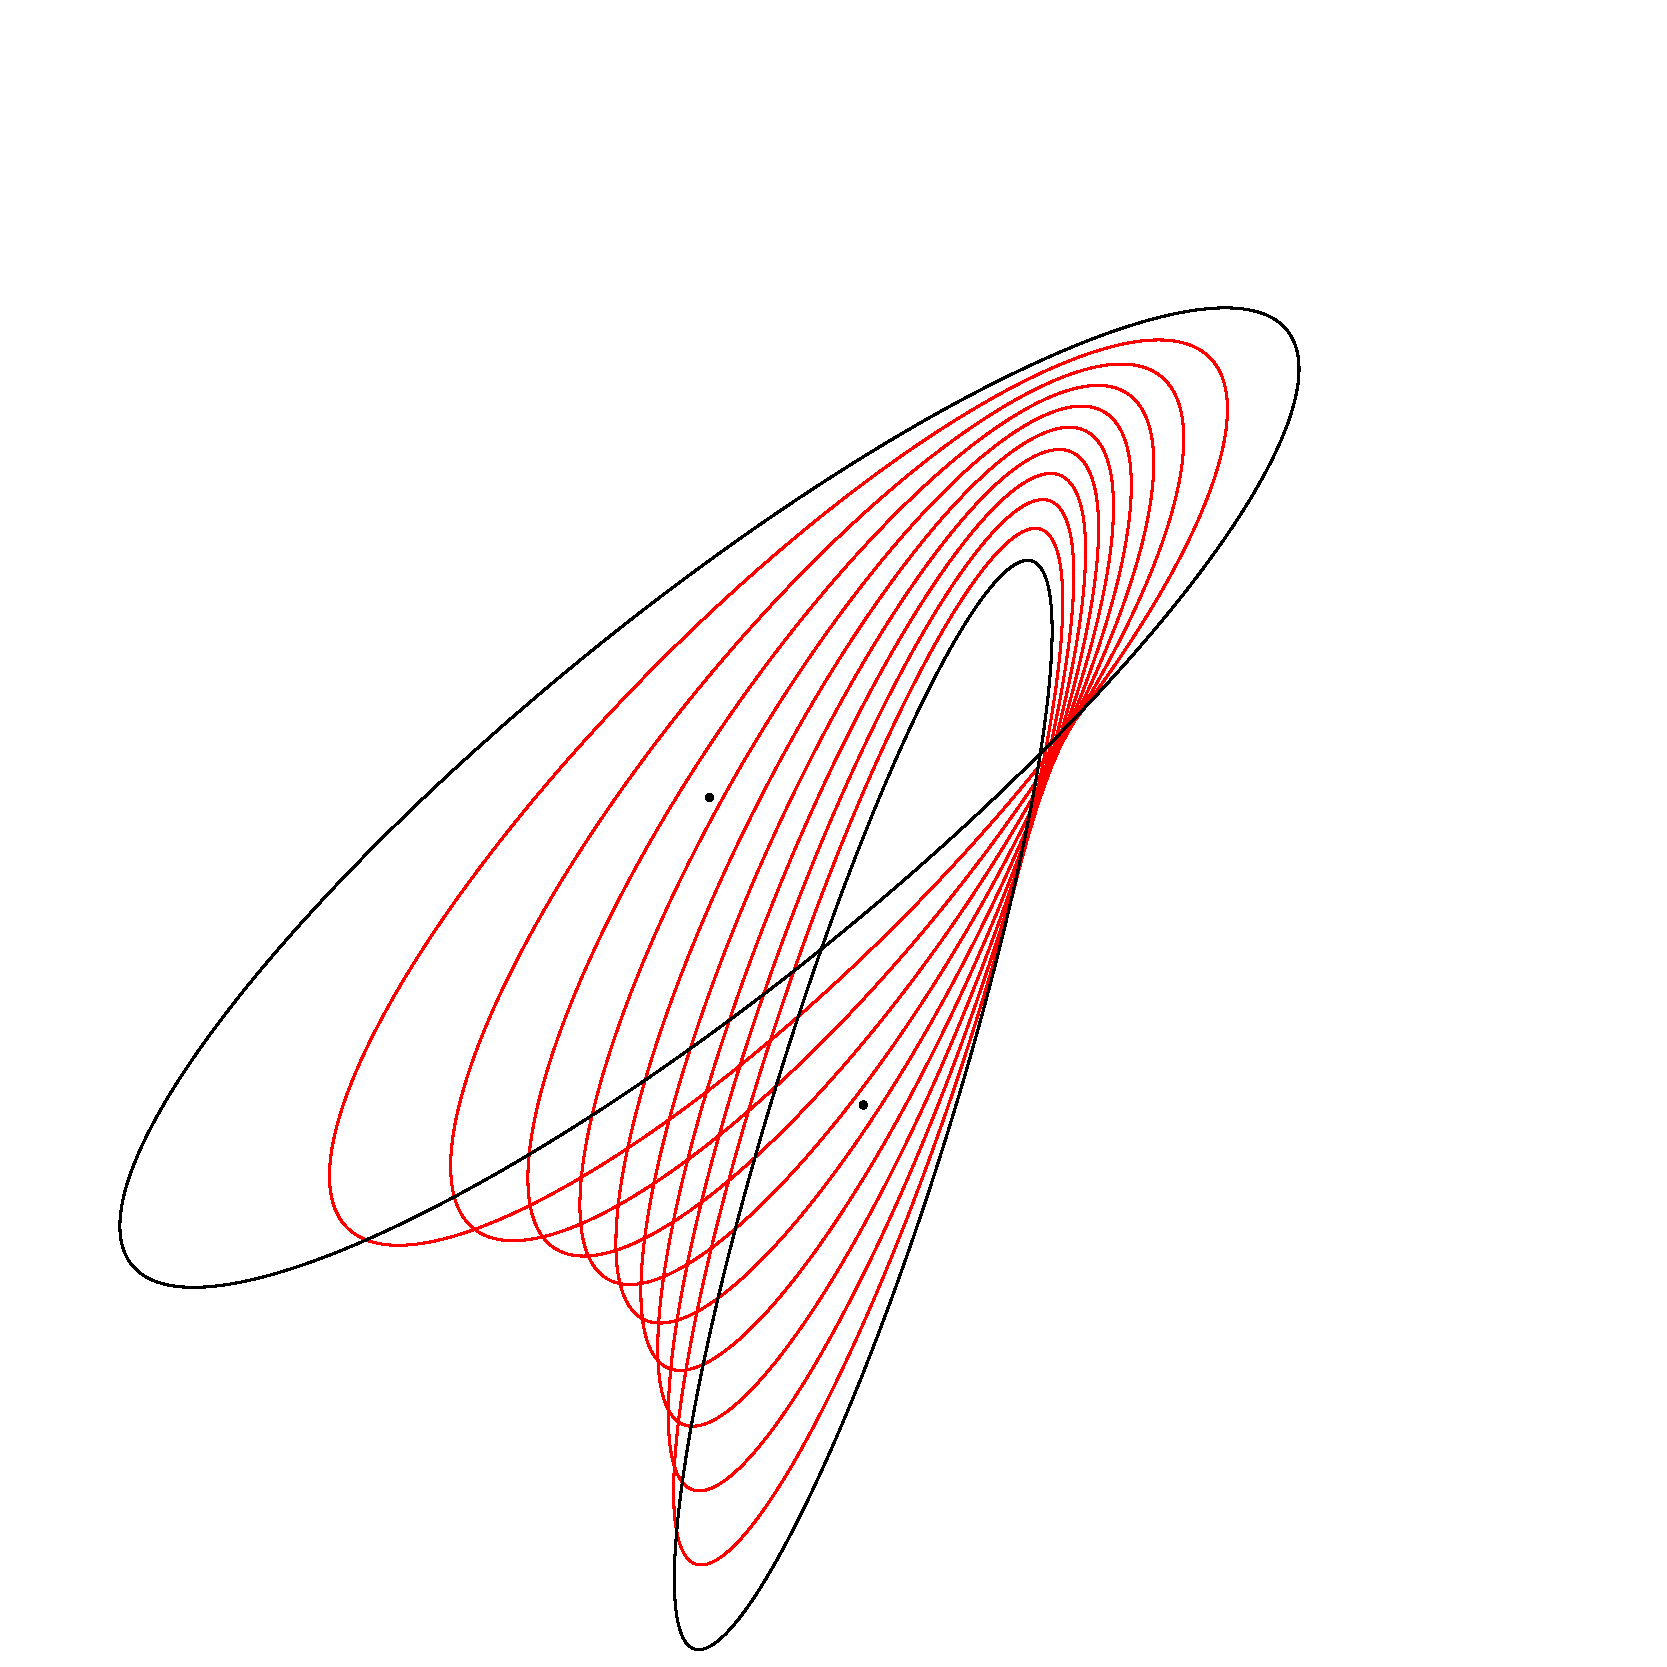
\includegraphics[width=0.2\textwidth]{BivariateNormal2-T.pdf} &
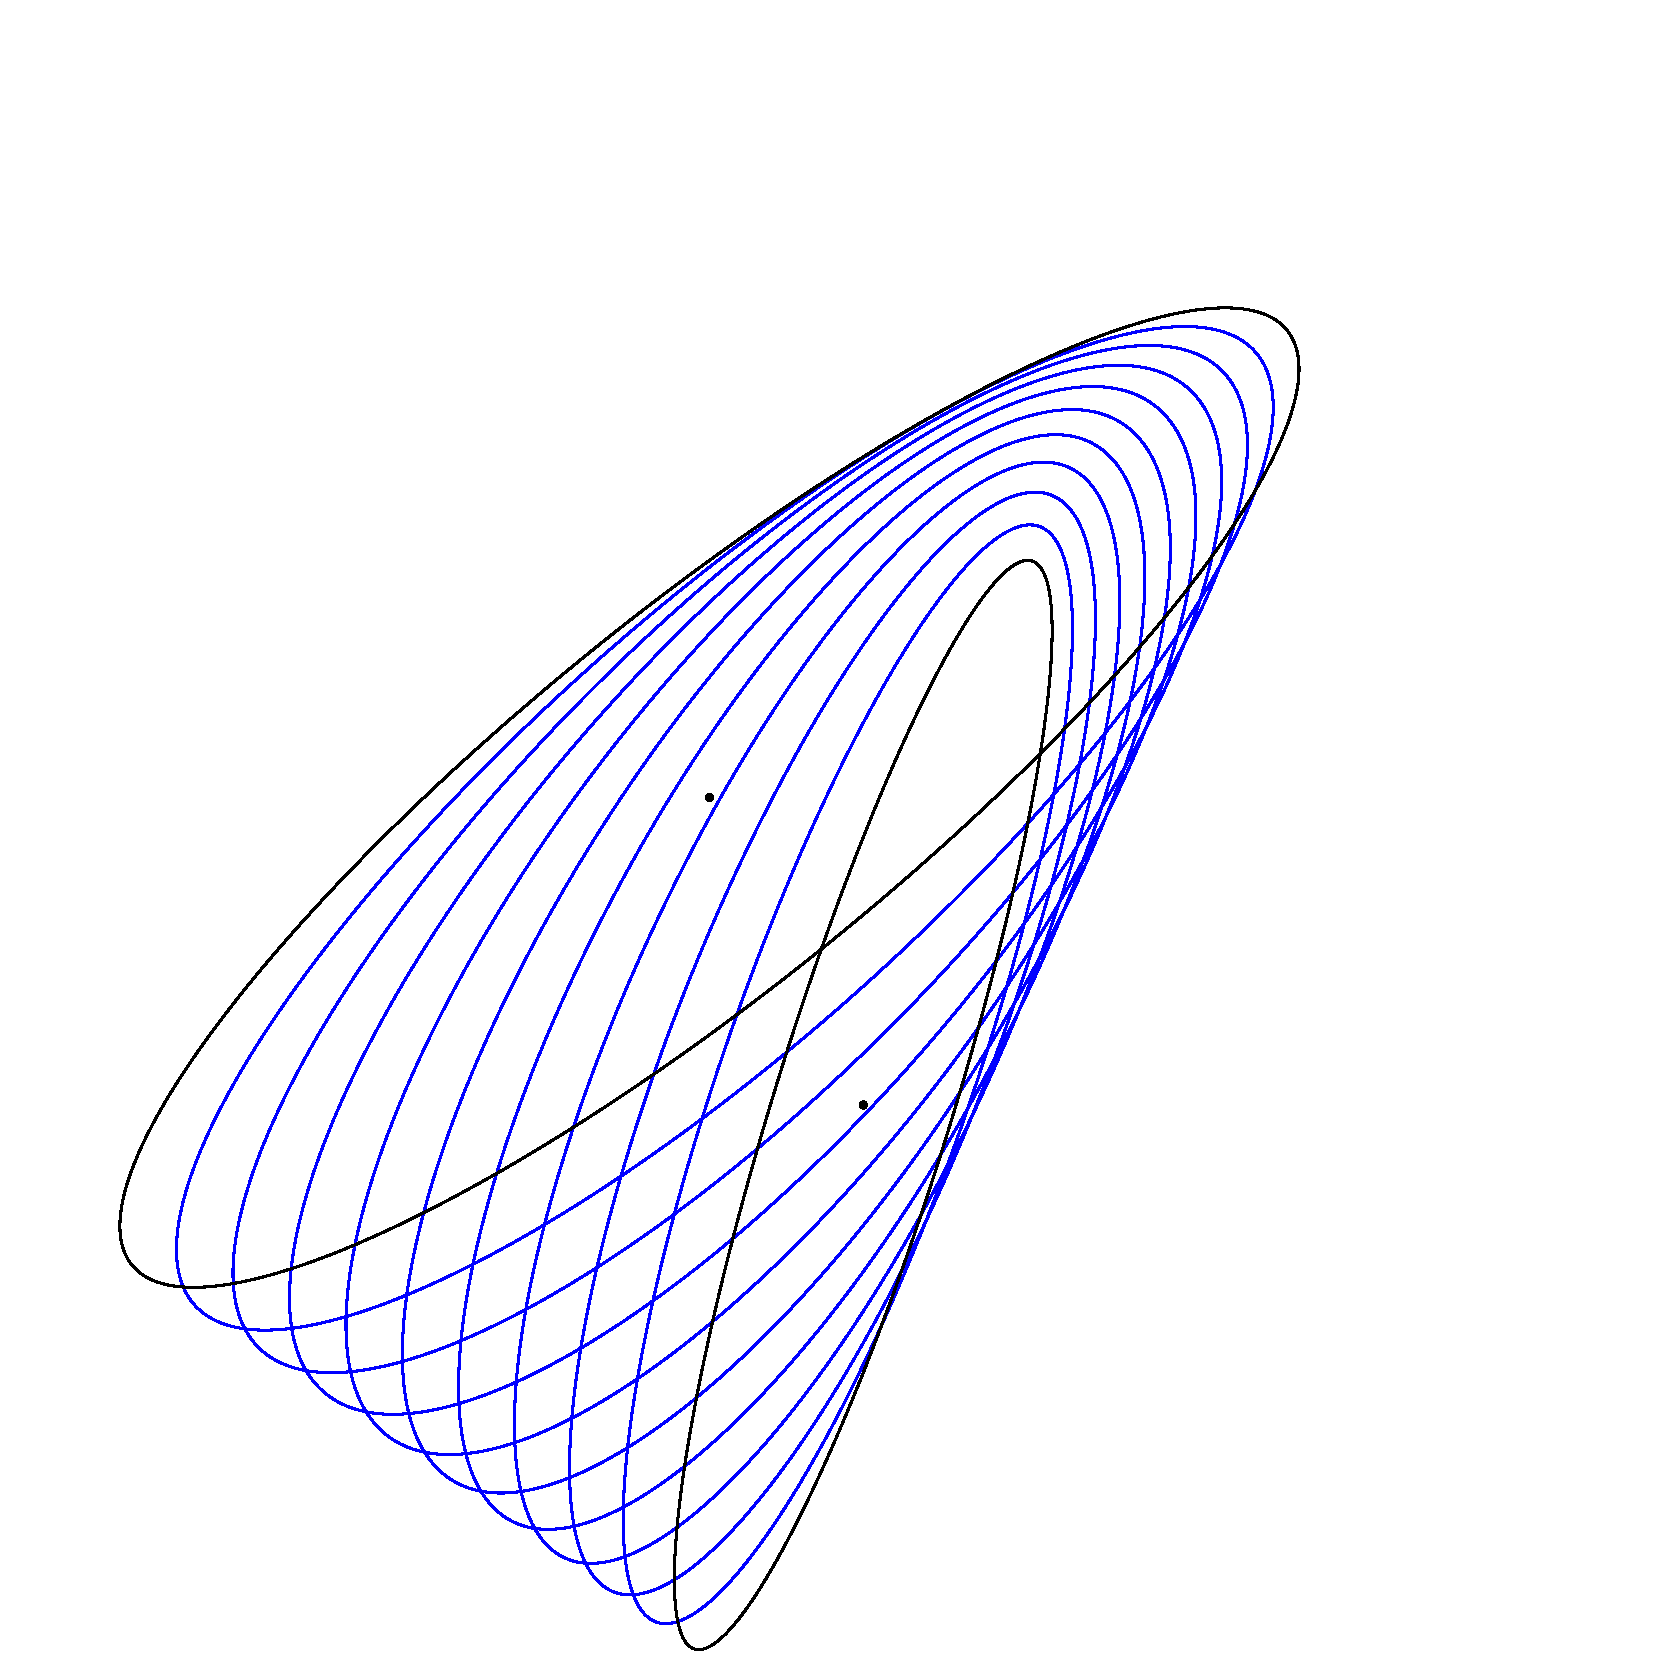
\includegraphics[width=0.2\textwidth]{BivariateNormal2-E.pdf}&
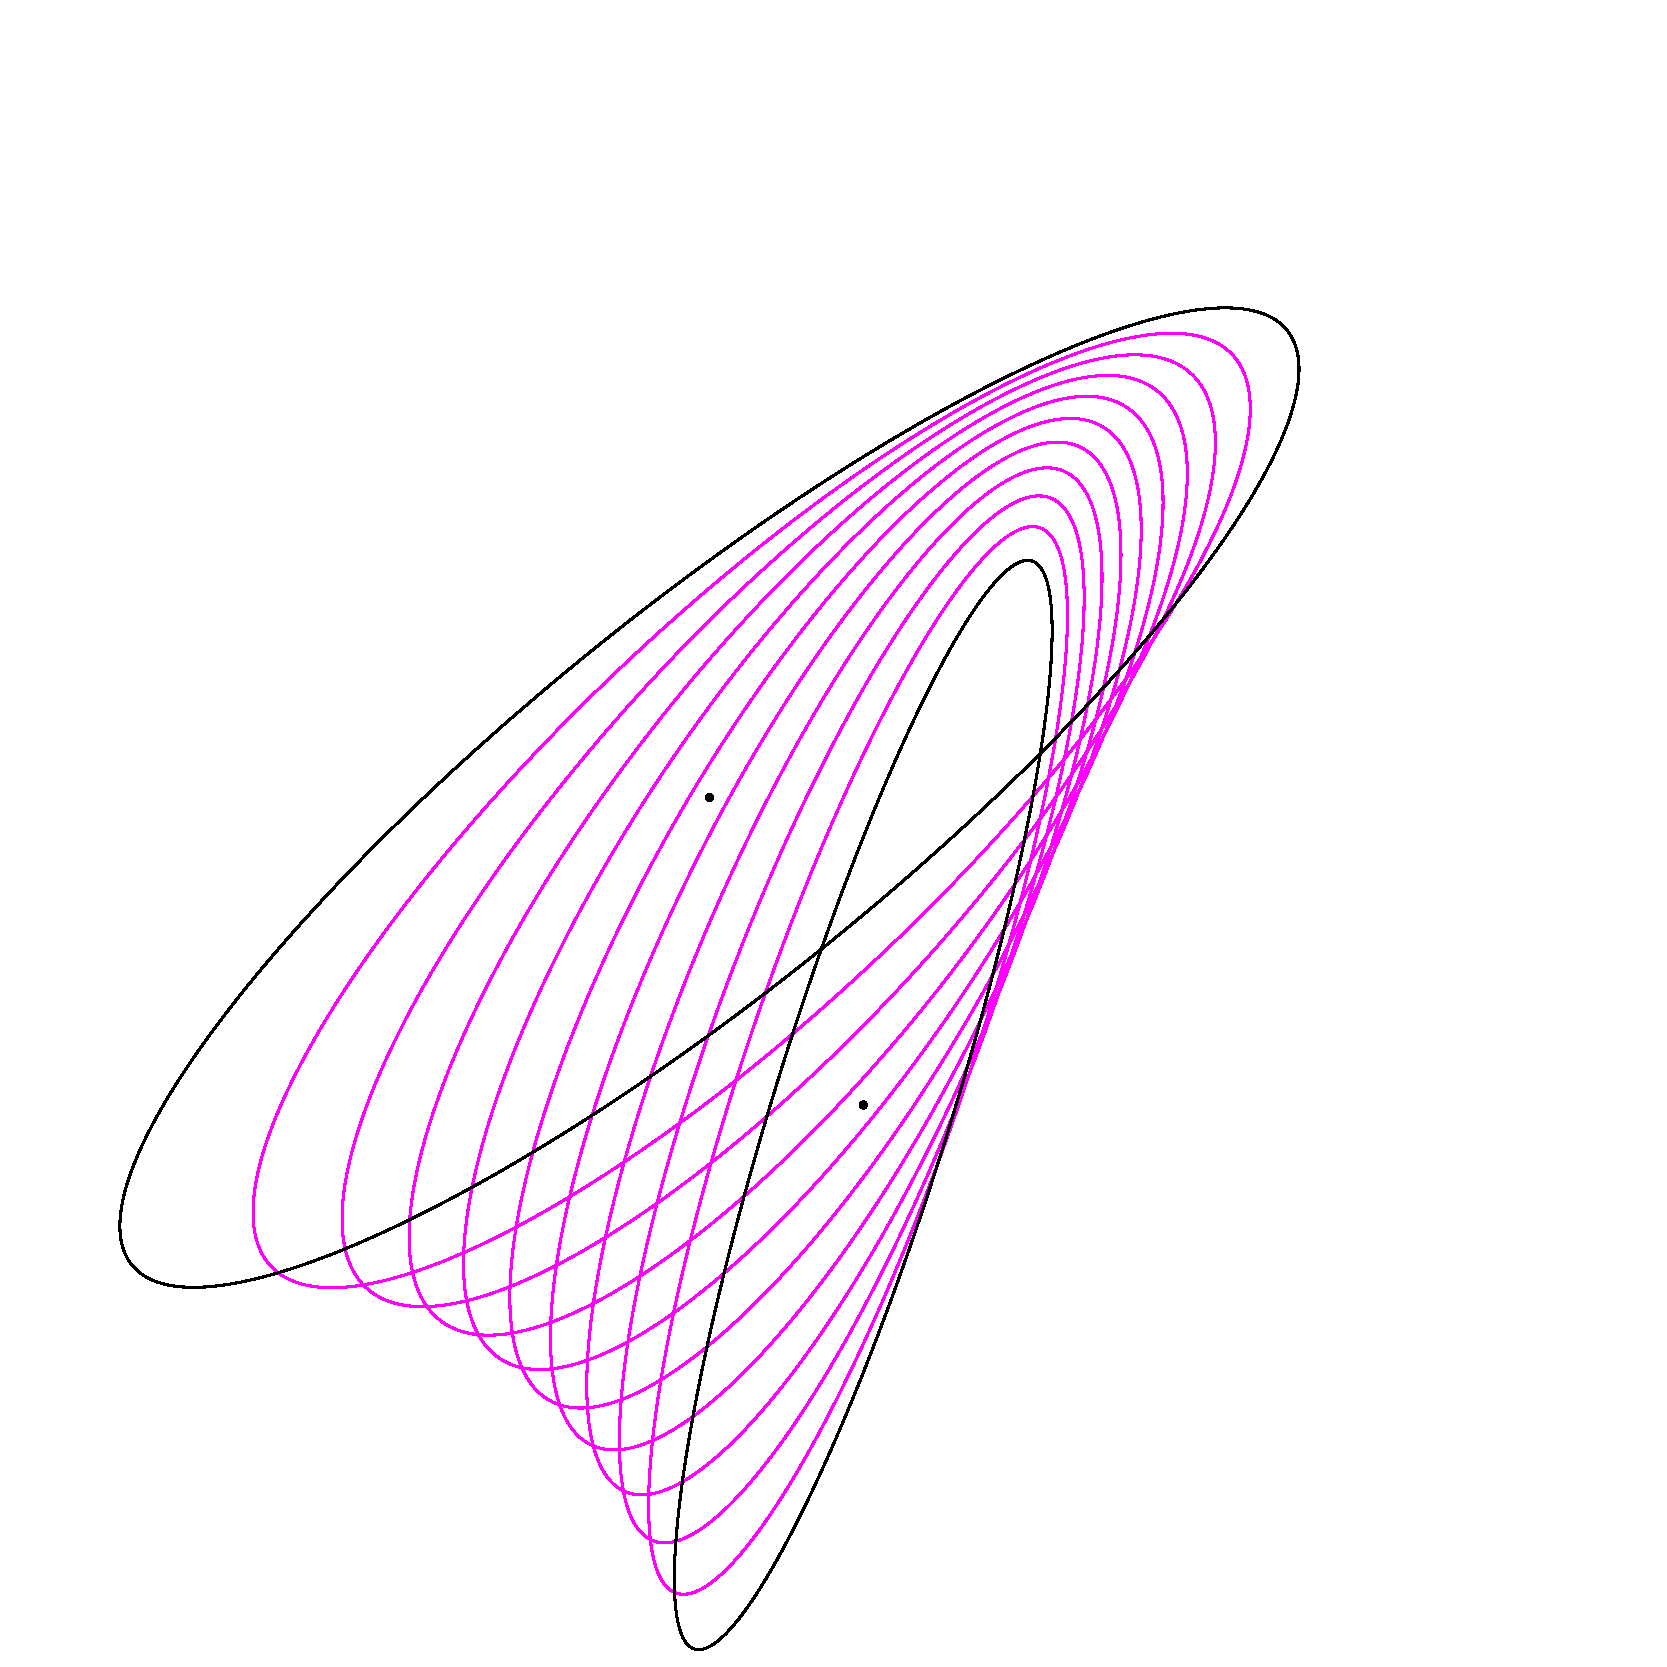
\includegraphics[width=0.2\textwidth]{BivariateNormal2-ET.pdf} \\
(\textbf{a}) & (\textbf{b}) & (\textbf{c})\cr
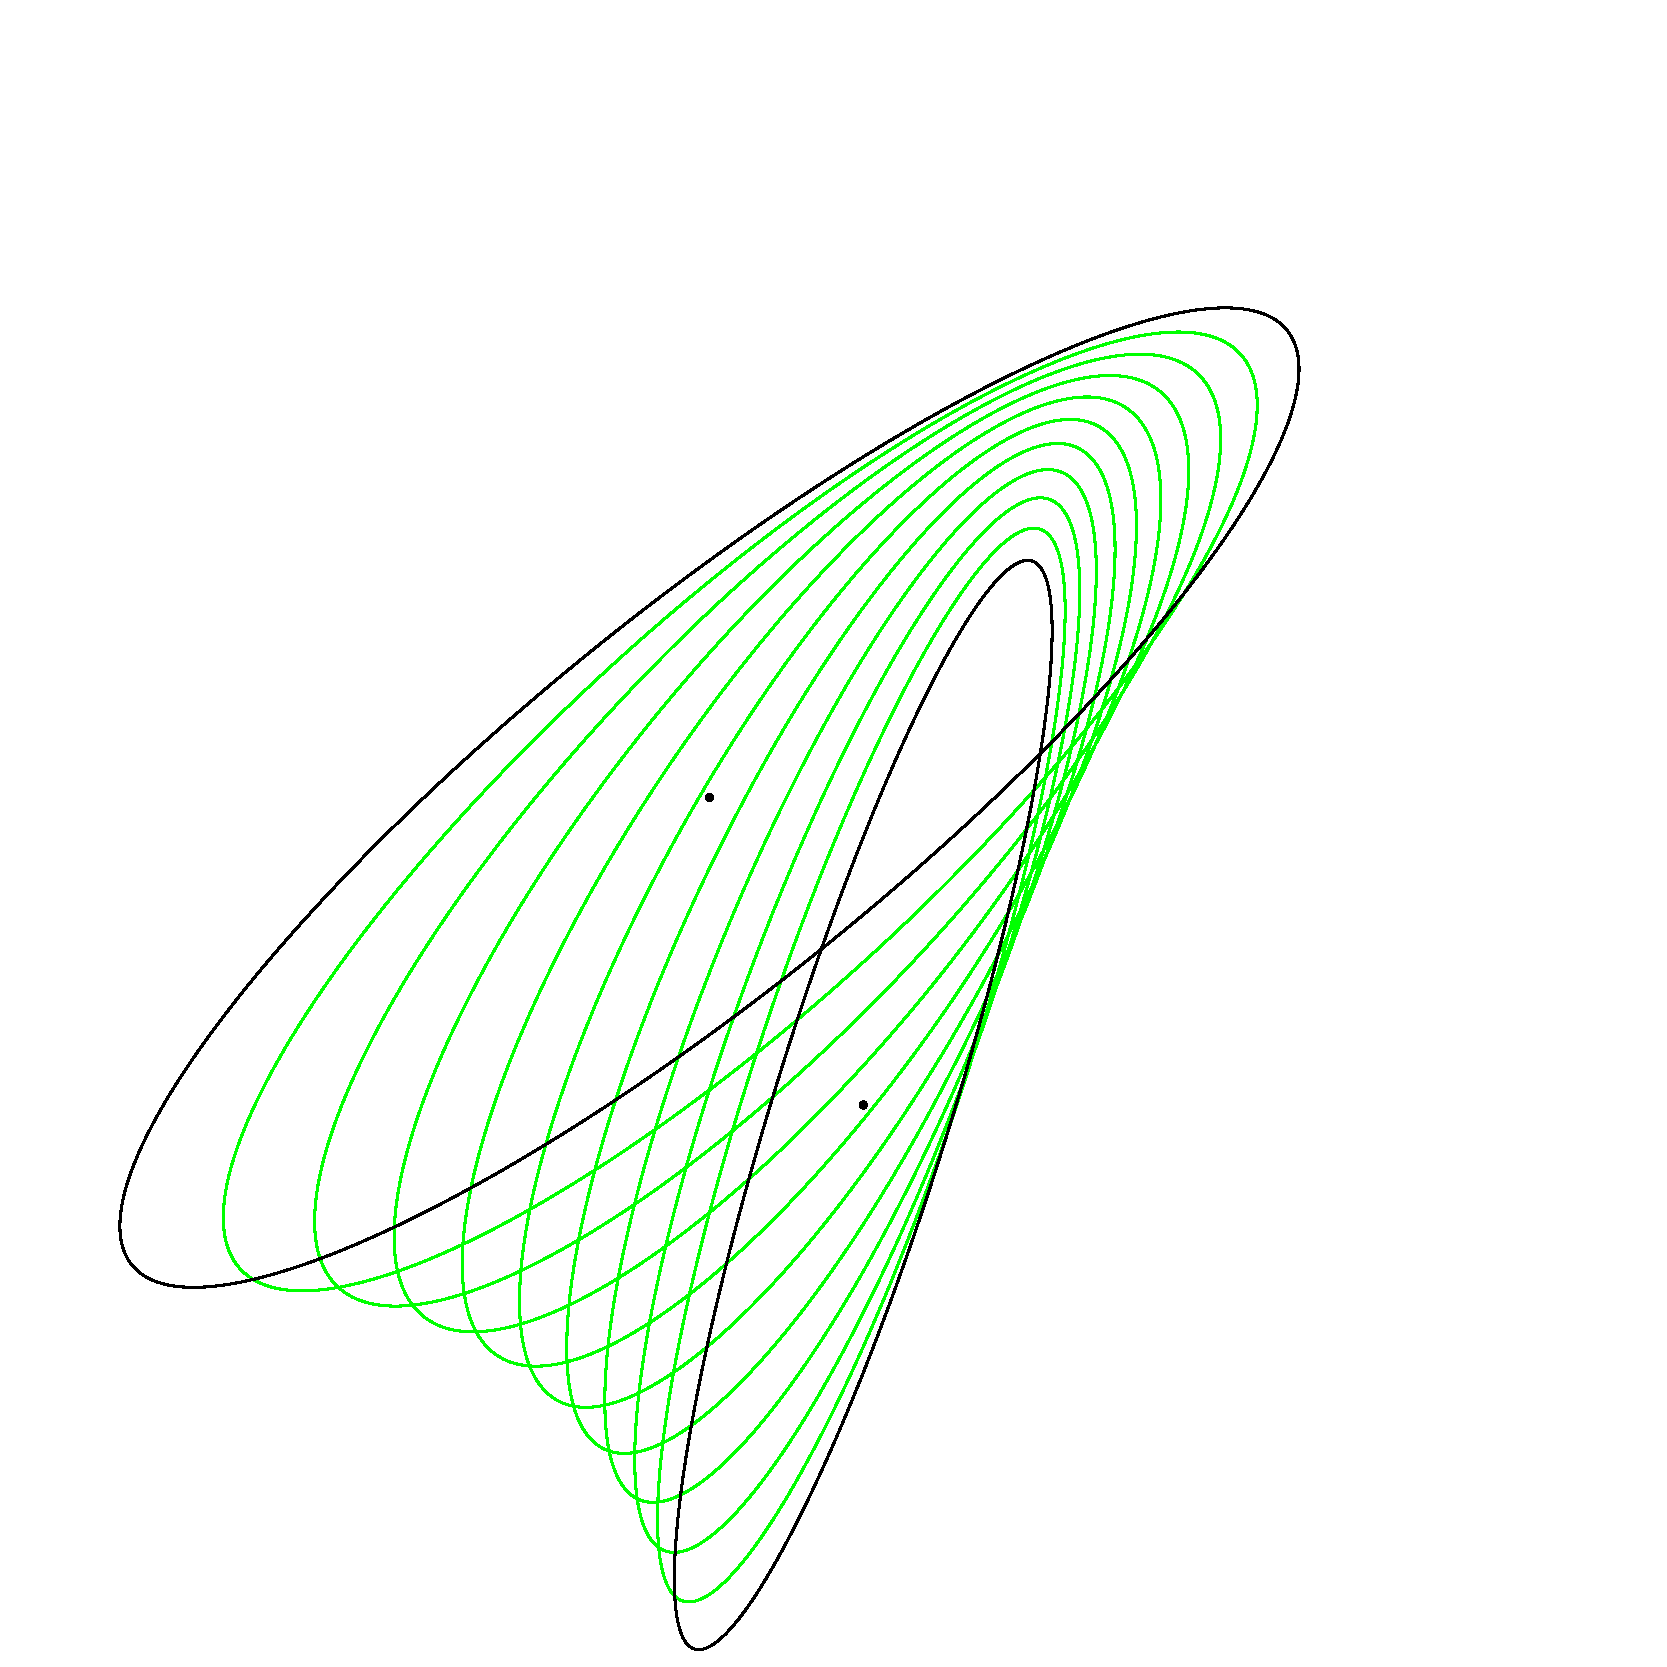
\includegraphics[width=0.2\textwidth]{BivariateNormal2-CO.pdf} &
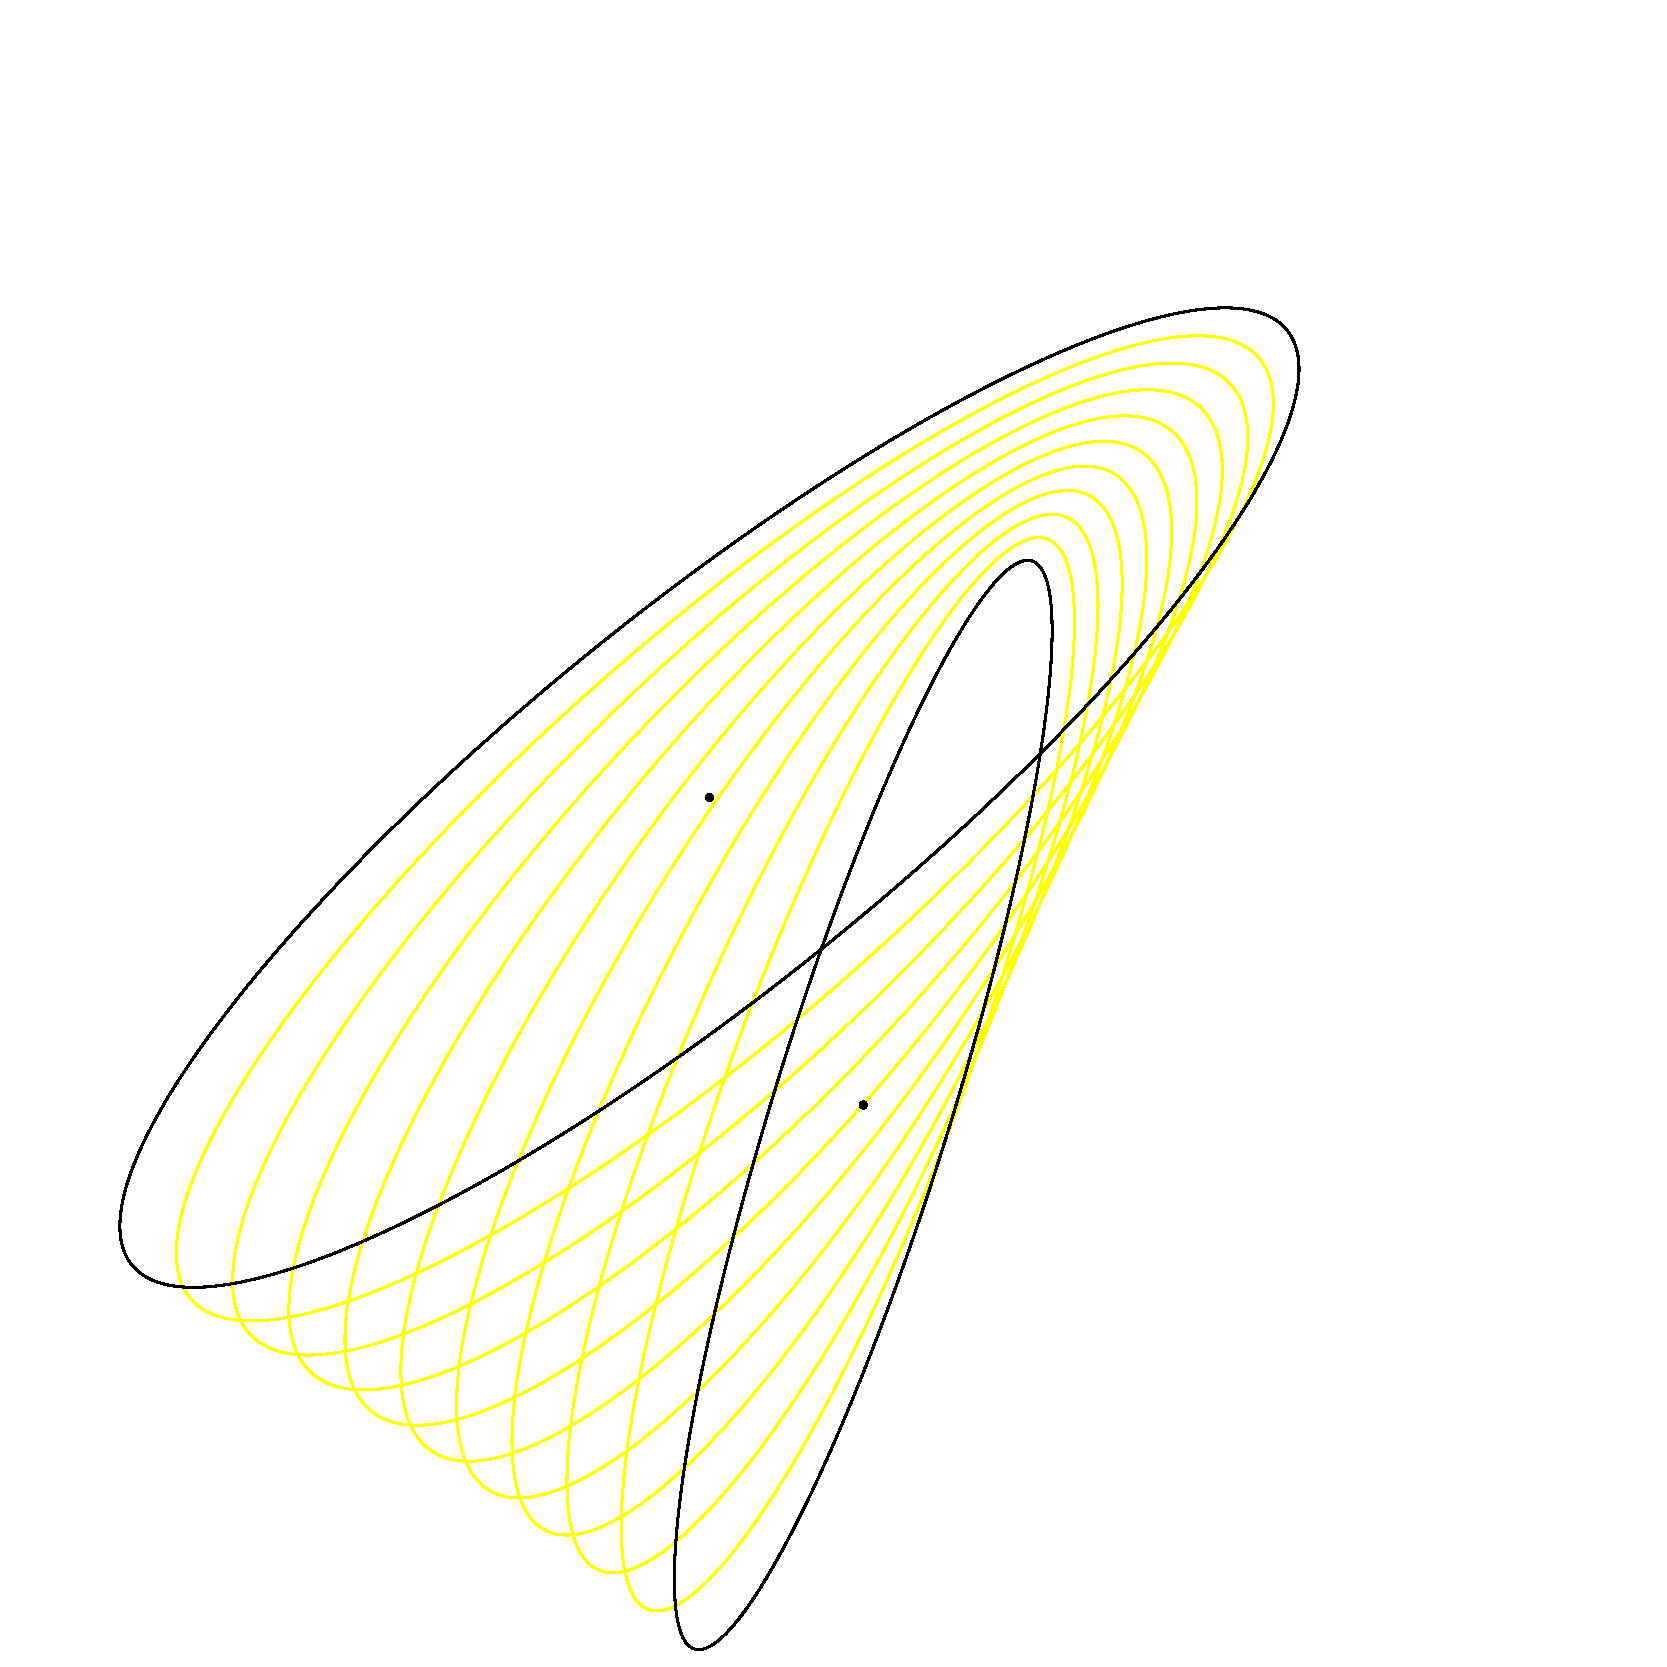
\includegraphics[width=0.2\textwidth]{BivariateNormal2-L.pdf} &
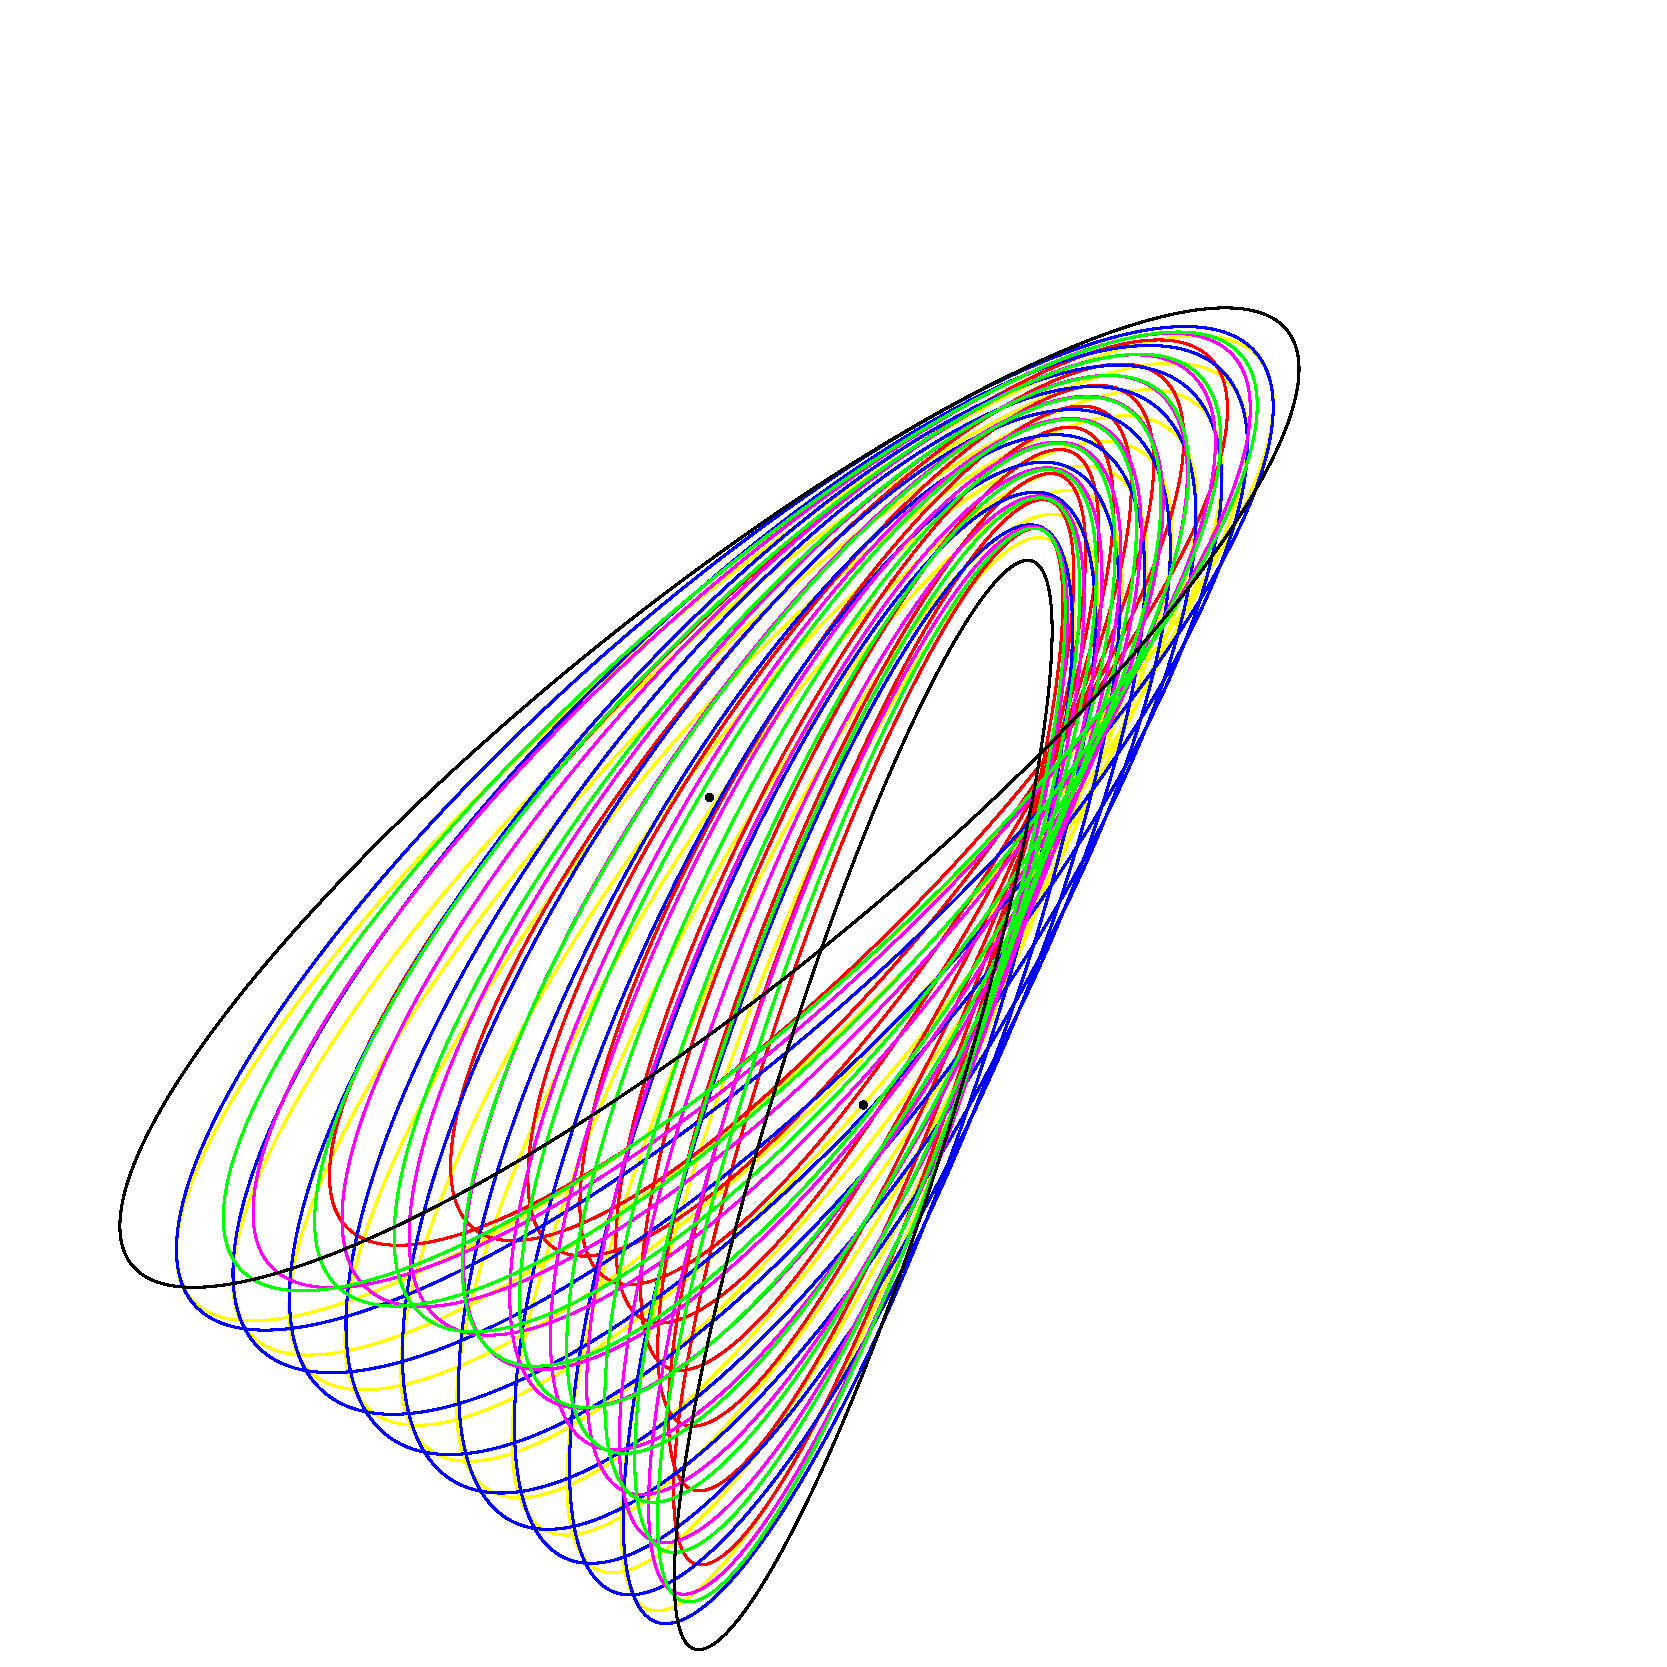
\includegraphics[width=0.2\textwidth]{BivariateNormal2-All.pdf} \\
(\textbf{d}) &(\textbf{e}) & (\textbf{f})
\end{tabular}
%
\caption{Visualizing at discrete positions (10 increment steps between $0$ and $1$) some curves used to approximate the Fisher–Rao distance between two bivariate normal distributions:
(\textbf{a}) exponential geodesic $c^e=\gamma_\calN^e$ (red),
(\textbf{b}) mixture geodesic $c^m=\gamma_\calN^m$ (blue),
(\textbf{c}) mid-mixture-exponential curve $c^{\mathrm{em}}$ (purple),
(\textbf{d}) projected Calvo and Oller curve $c^{\CO}$ (green), 
(\textbf{e}) $c^\lambda$: ordinary linear interpolation in $\lambda$ (yellow),
and
(\textbf{f}) All superposed curves at once.
 \label{fig:viz2Dbis}}
\end{figure}





\begin{Example}
Let us report some numerical results for bivariate normals with $T=1000$: 

\begin{itemize}


\item We use the following example of Han and Park~\cite{MVNGeodesicShooting-2014} ({Equation (26)}%Yes, of ref 39 MDPI: Please check if this Equation belongs to Ref.39, if not, please add the link of this Equation here.
):
$$
N_1=\left(\vectortwo{0}{0},\mattwotwo{1}{0}{0}{0.1}\right),\quad
N_2=\left(\vectortwo{1}{1},\mattwotwo{0.1}{0}{0}{1}\right).
$$
Their geodesic shooting algorithm~\cite{MVNGeodesicShooting-2014} evaluates the Fisher–Rao distance to 
$\rho_\calN(N_1,N_2) \approx \mathbf{3.1329}$ (precision $10^{-5}$).

We~obtain:
\begin{itemize}
	\item Calvo and Oller lower bound: $\rho_\CO(N_1,N_2)\approx \mathbf{3.0470}$,
	\item Upper bound using Equation~(\ref{eq:UBMah}): $7.92179$,
	\item SPC upper bound~(Equation~(\ref{prop:USPC})): $U_\SPC(N_1,N_2)\approx 5.4302$,
	\item $\sqrt{D_J}$ upper bound: $U_{\sqrt{J}}(N_1,N_2)\approx \mathbf{4.3704}$,
	\item $\tilde\rho_\calN^\lambda(N_1,N_2)\approx 3.4496$,
	\item $\tilde\rho_\calN^m(N_1,N_2)\approx 3.5775$,
	\item $\tilde\rho_\calN^e(N_1,N_2)\approx 3.7314$,
	\item $\tilde\rho_\calN^{\mathrm{em}}(N_1,N_2)\approx 3.1672$,
	\item $\tilde\rho_\calN^{\CO}(N_1,N_2)\approx \mathbf{3.1391}$.
\end{itemize}
In that setting, the~$\sqrt{D_J}$ upper bound is better than the upper bound of Equation~(\ref{prop:USPC}), and~the projected Calvo and Oller geodesic yields the best approximation of the Fisher–Rao distance (Figure~\ref{Fig:HanPark}) with an absolute error of $0.0062$ (about $0.2\%$ relative error).
When $T=10$, we have  $\tilde\rho_\calN^{\CO}(N_1,N_2)\approx 3.1530$, when $T=100$, we obtain  $\tilde\rho_\calN^{\CO}(N_1,N_2)\approx 3.1136$, and~when $T=500$ we obtain $\tilde\rho_\calN^{\CO}(N_1,N_2)\approx 3.1362$ (which is better than the approximation obtained for $T=1000$).
Figure~\ref{Fig:HanParkRangeT} shows the fluctuations of the approximation of the Fisher–Rao distance by the projected C\&O curve when $T$ ranges from $3$ to $100$.


\begin{figure}[H]

\begin{tabular}{cc}
%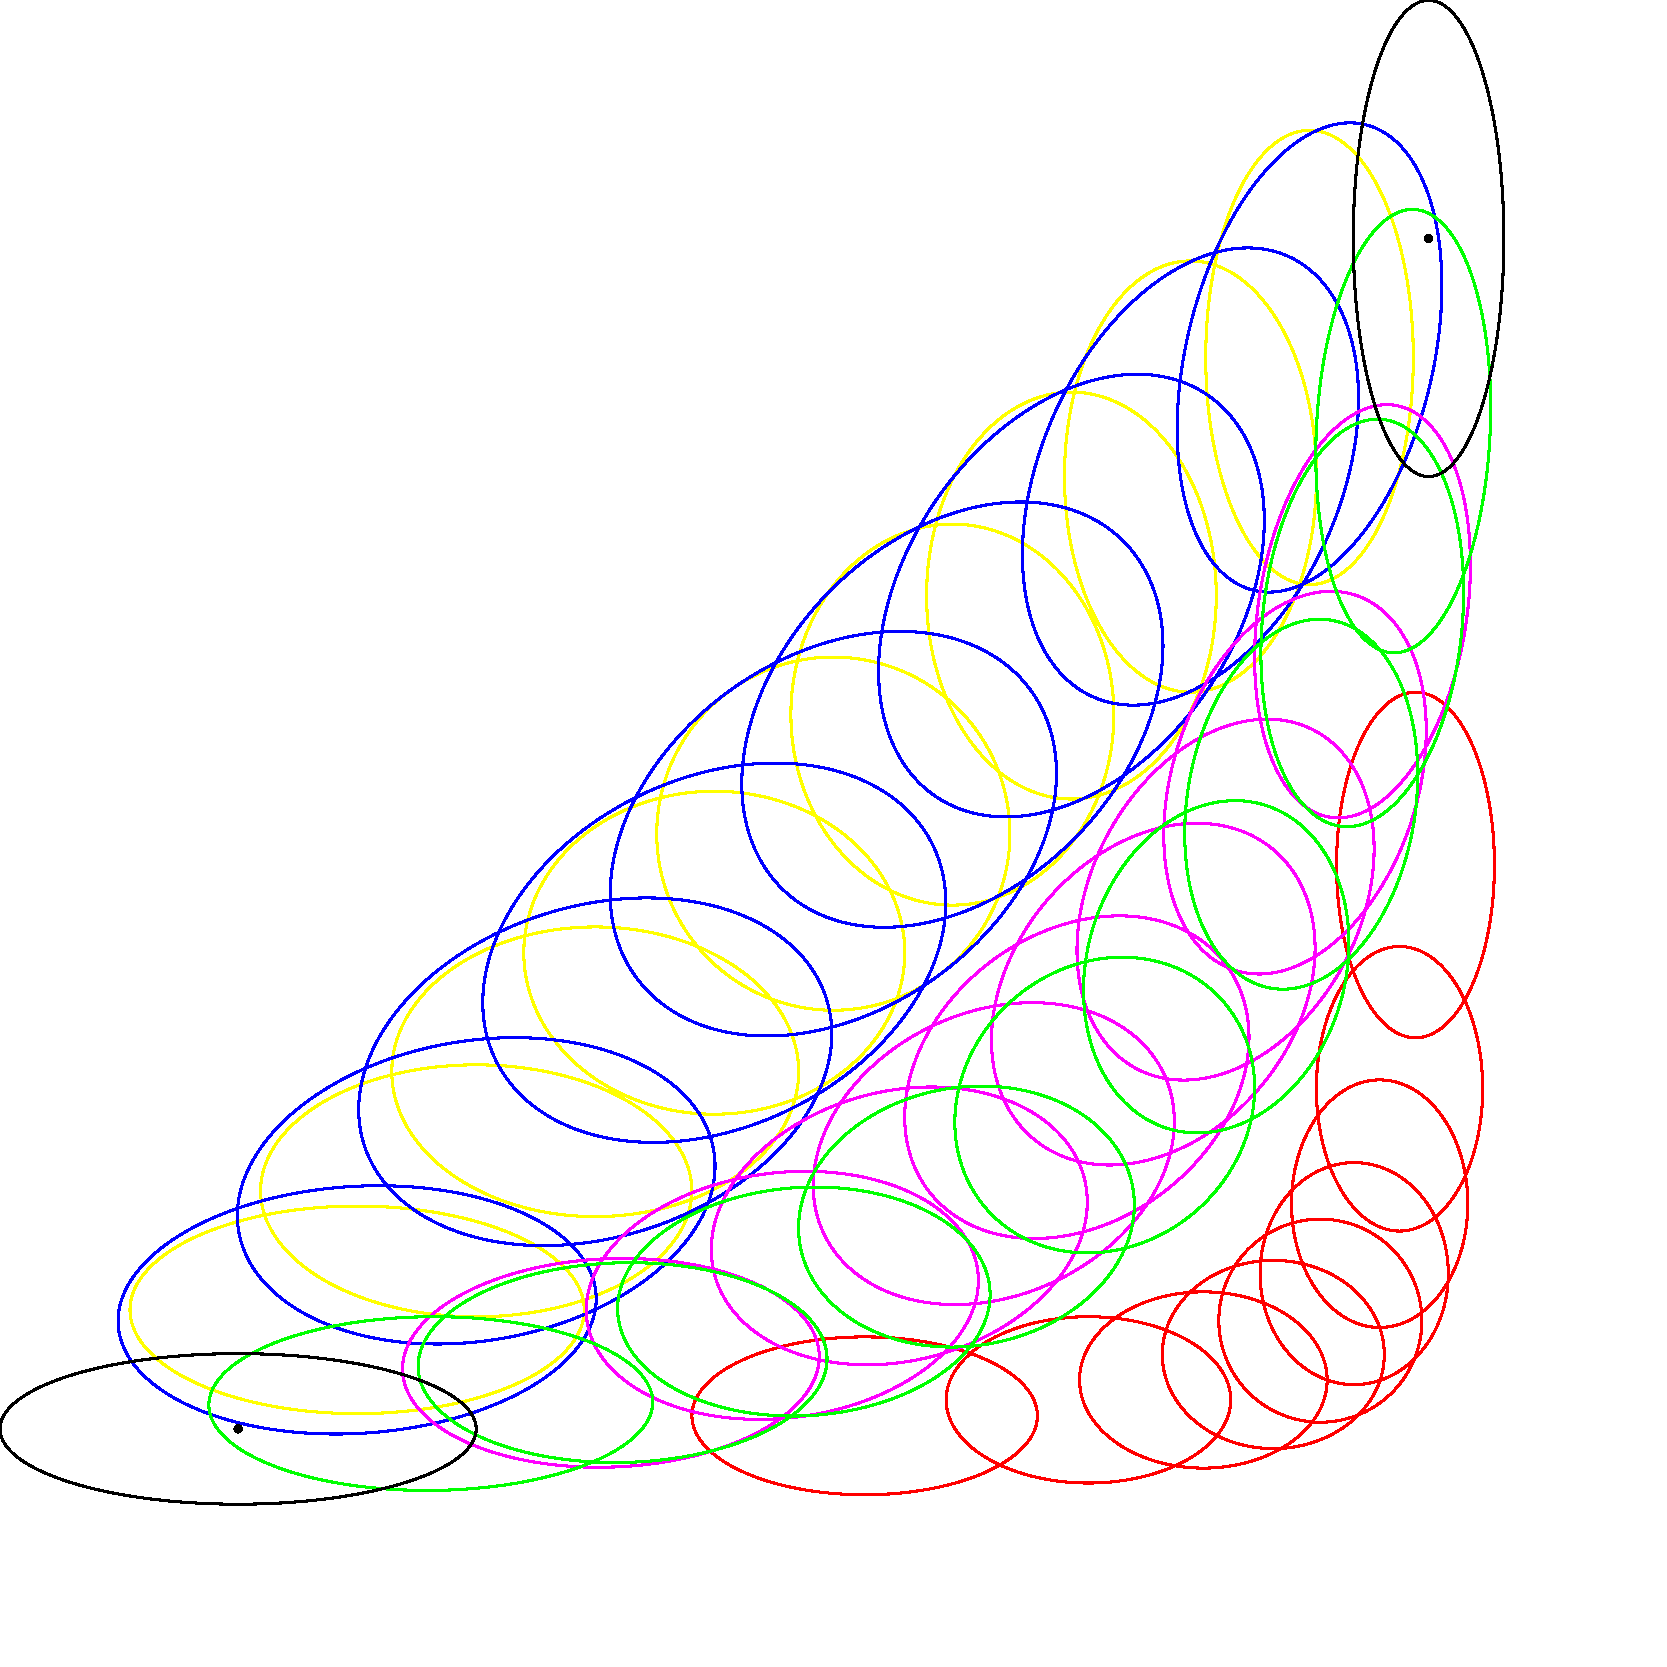
\includegraphics[width=0.3\textwidth]{BivariateNormal-ExHanPark.pdf} &
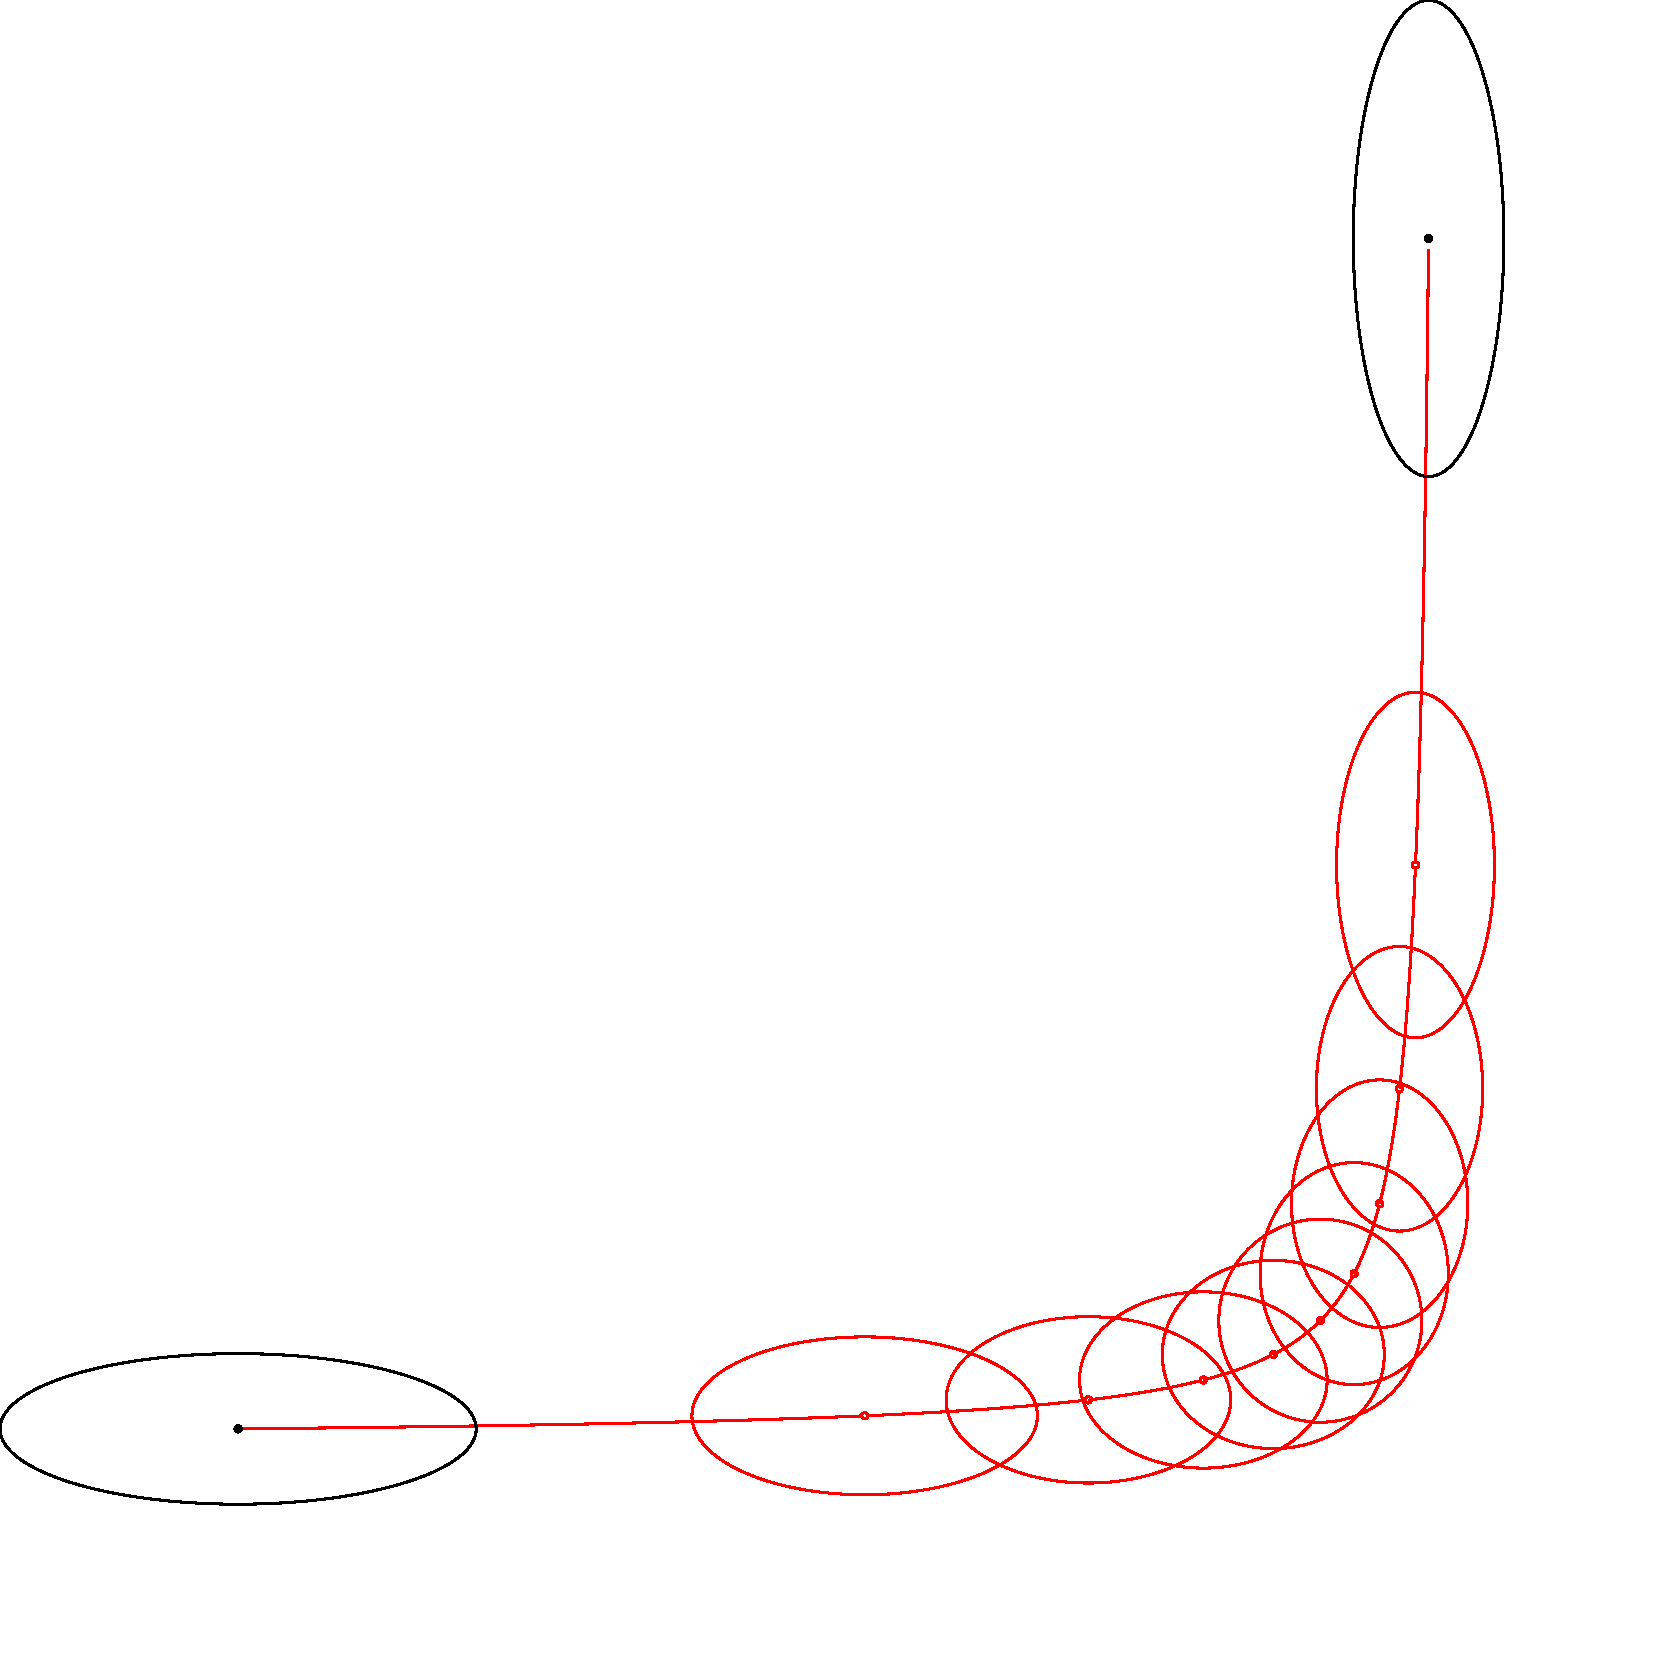
\includegraphics[width=0.25\textwidth]{BivariateNormal-52740-T.pdf} &
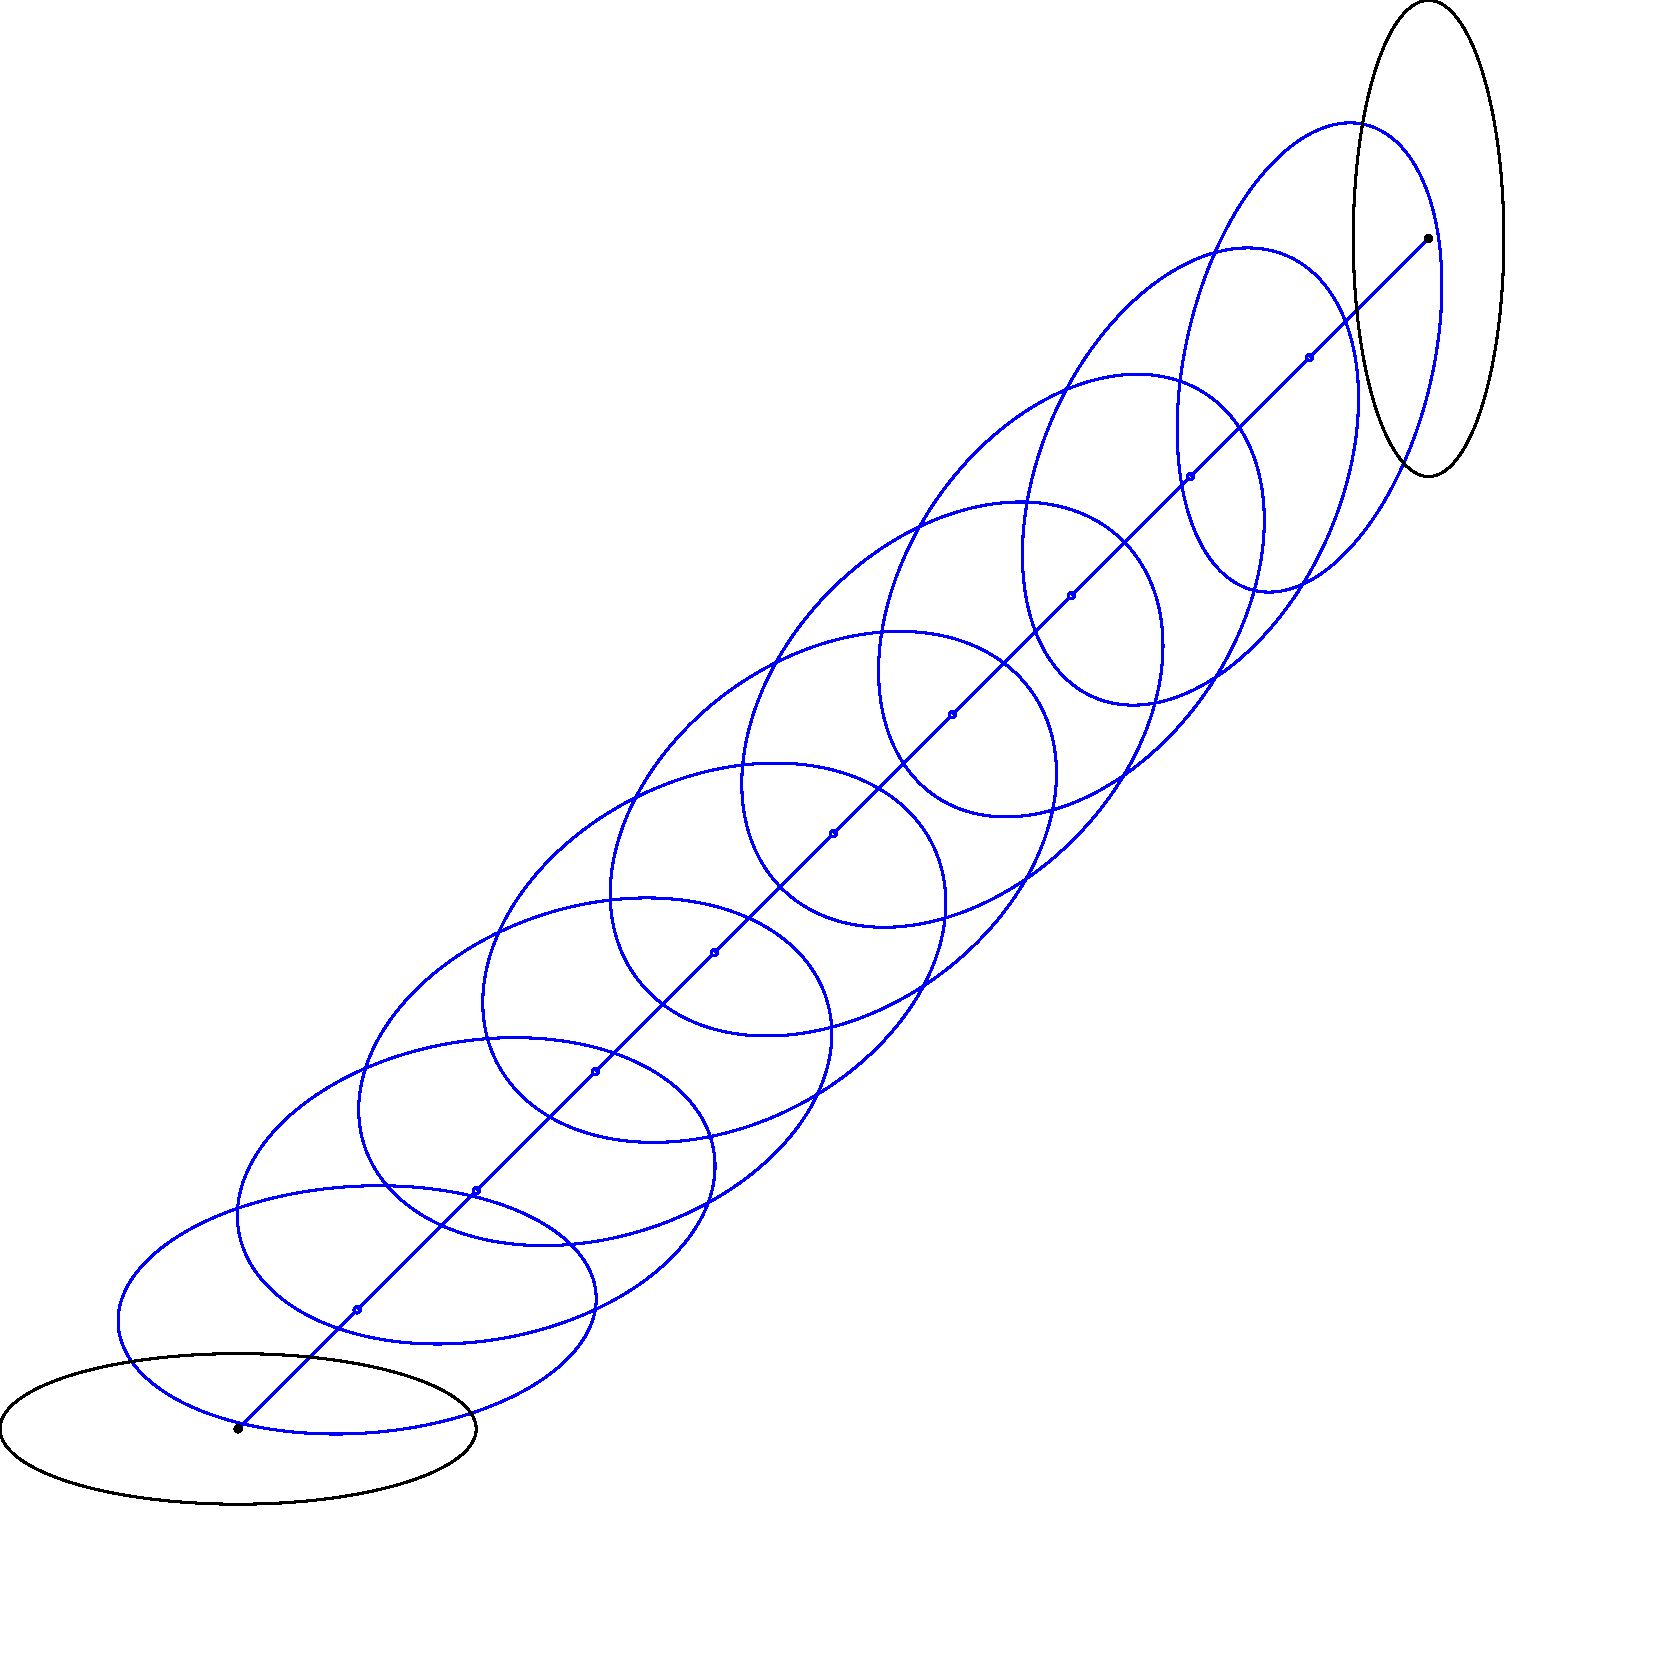
\includegraphics[width=0.25\textwidth]{BivariateNormal-52740-E.pdf} \\
(\textbf{a}) exponential geodesic & (\textbf{b}) mixture geodesic \\
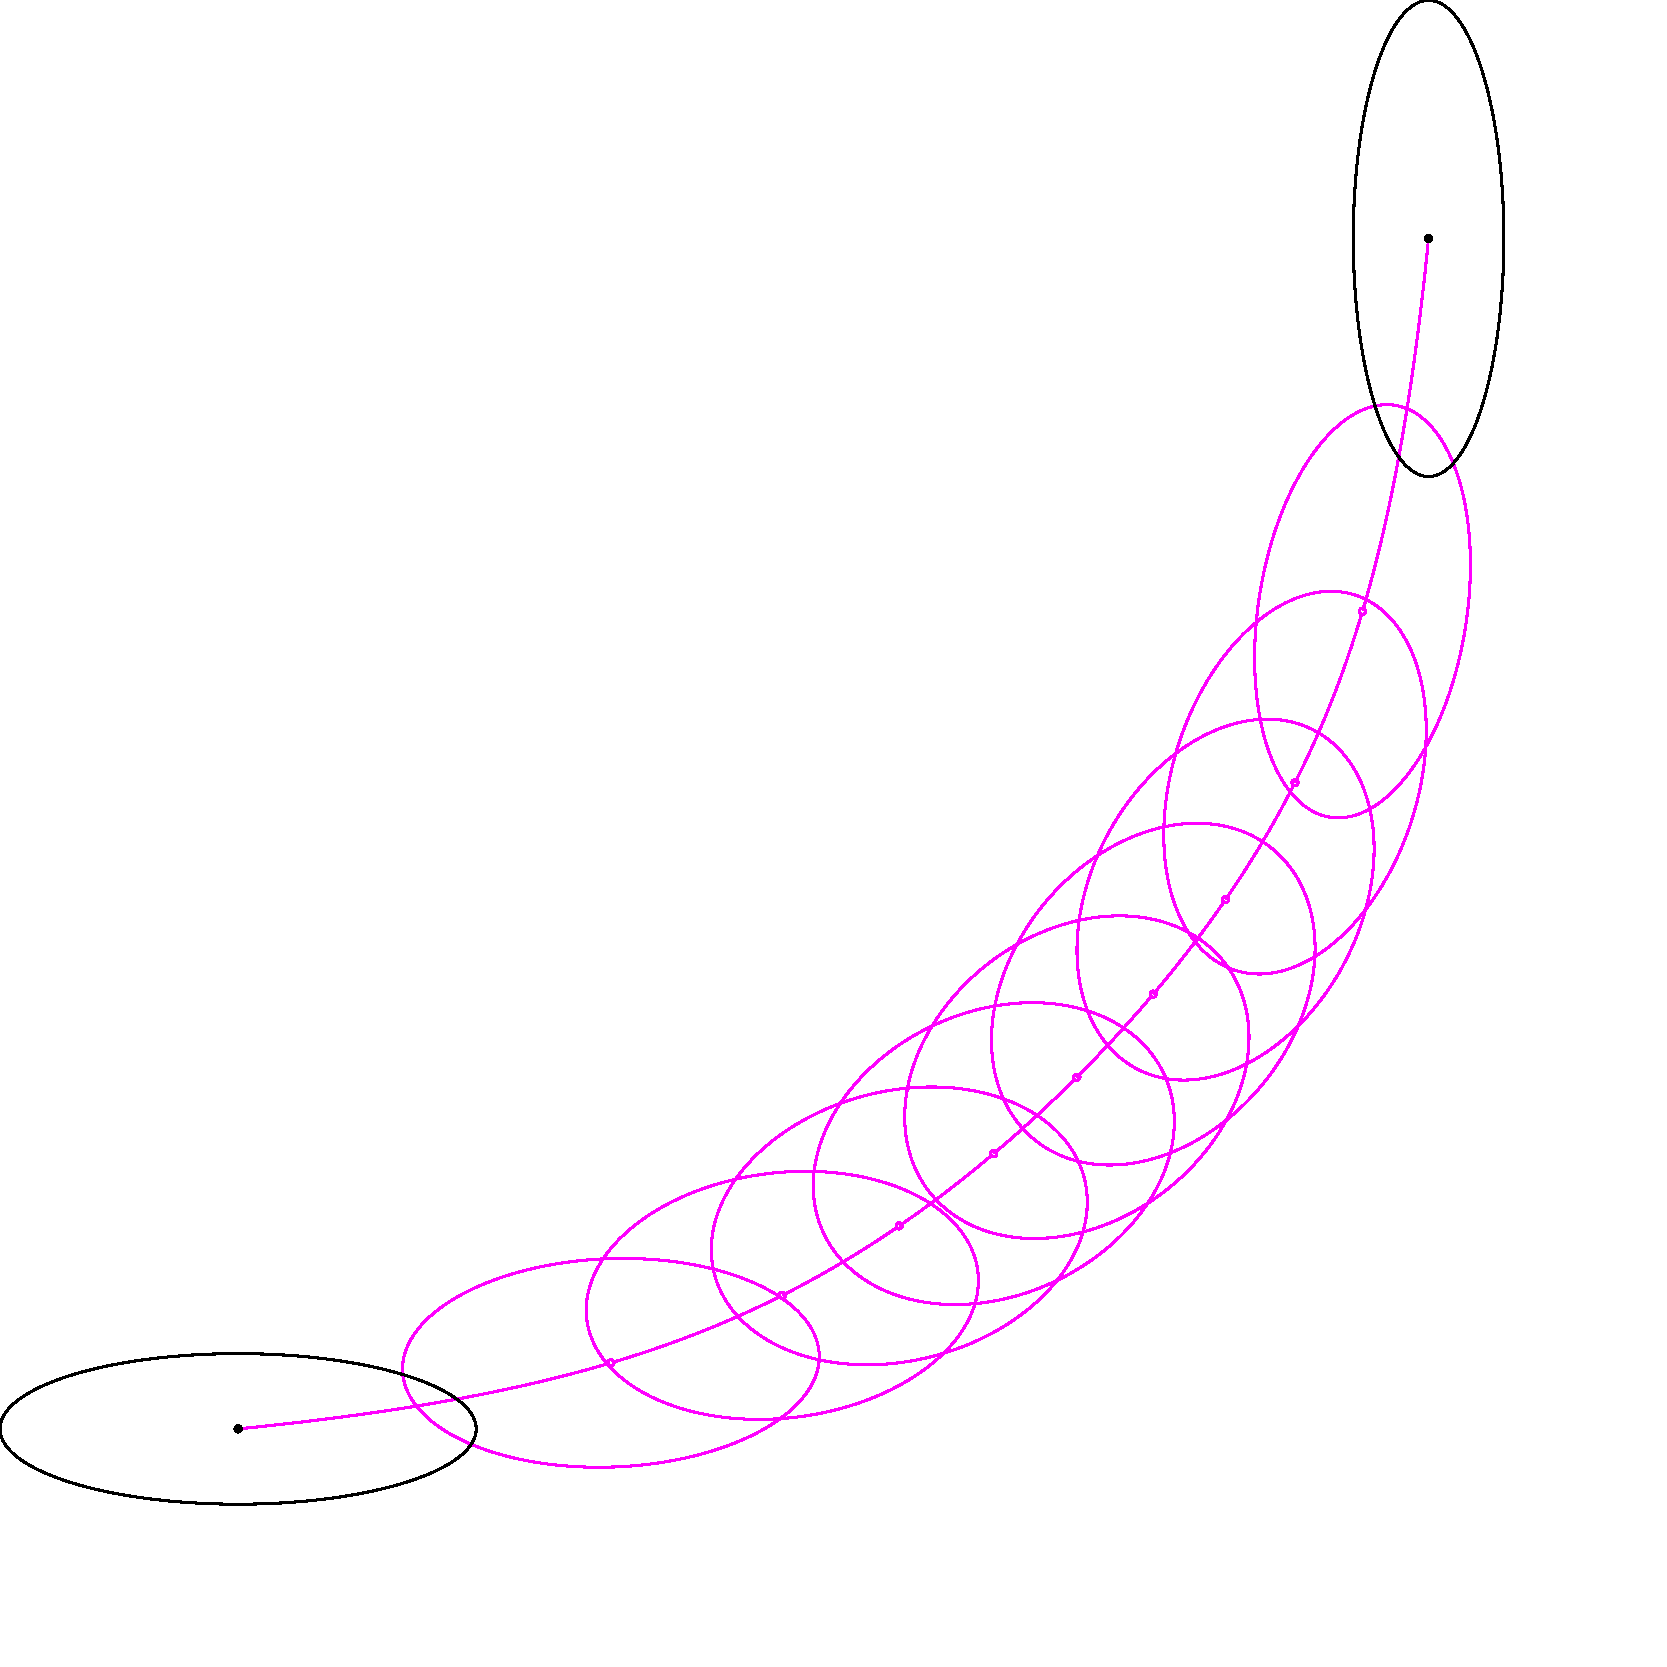
\includegraphics[width=0.25\textwidth]{BivariateNormal-52740-ET.pdf} &
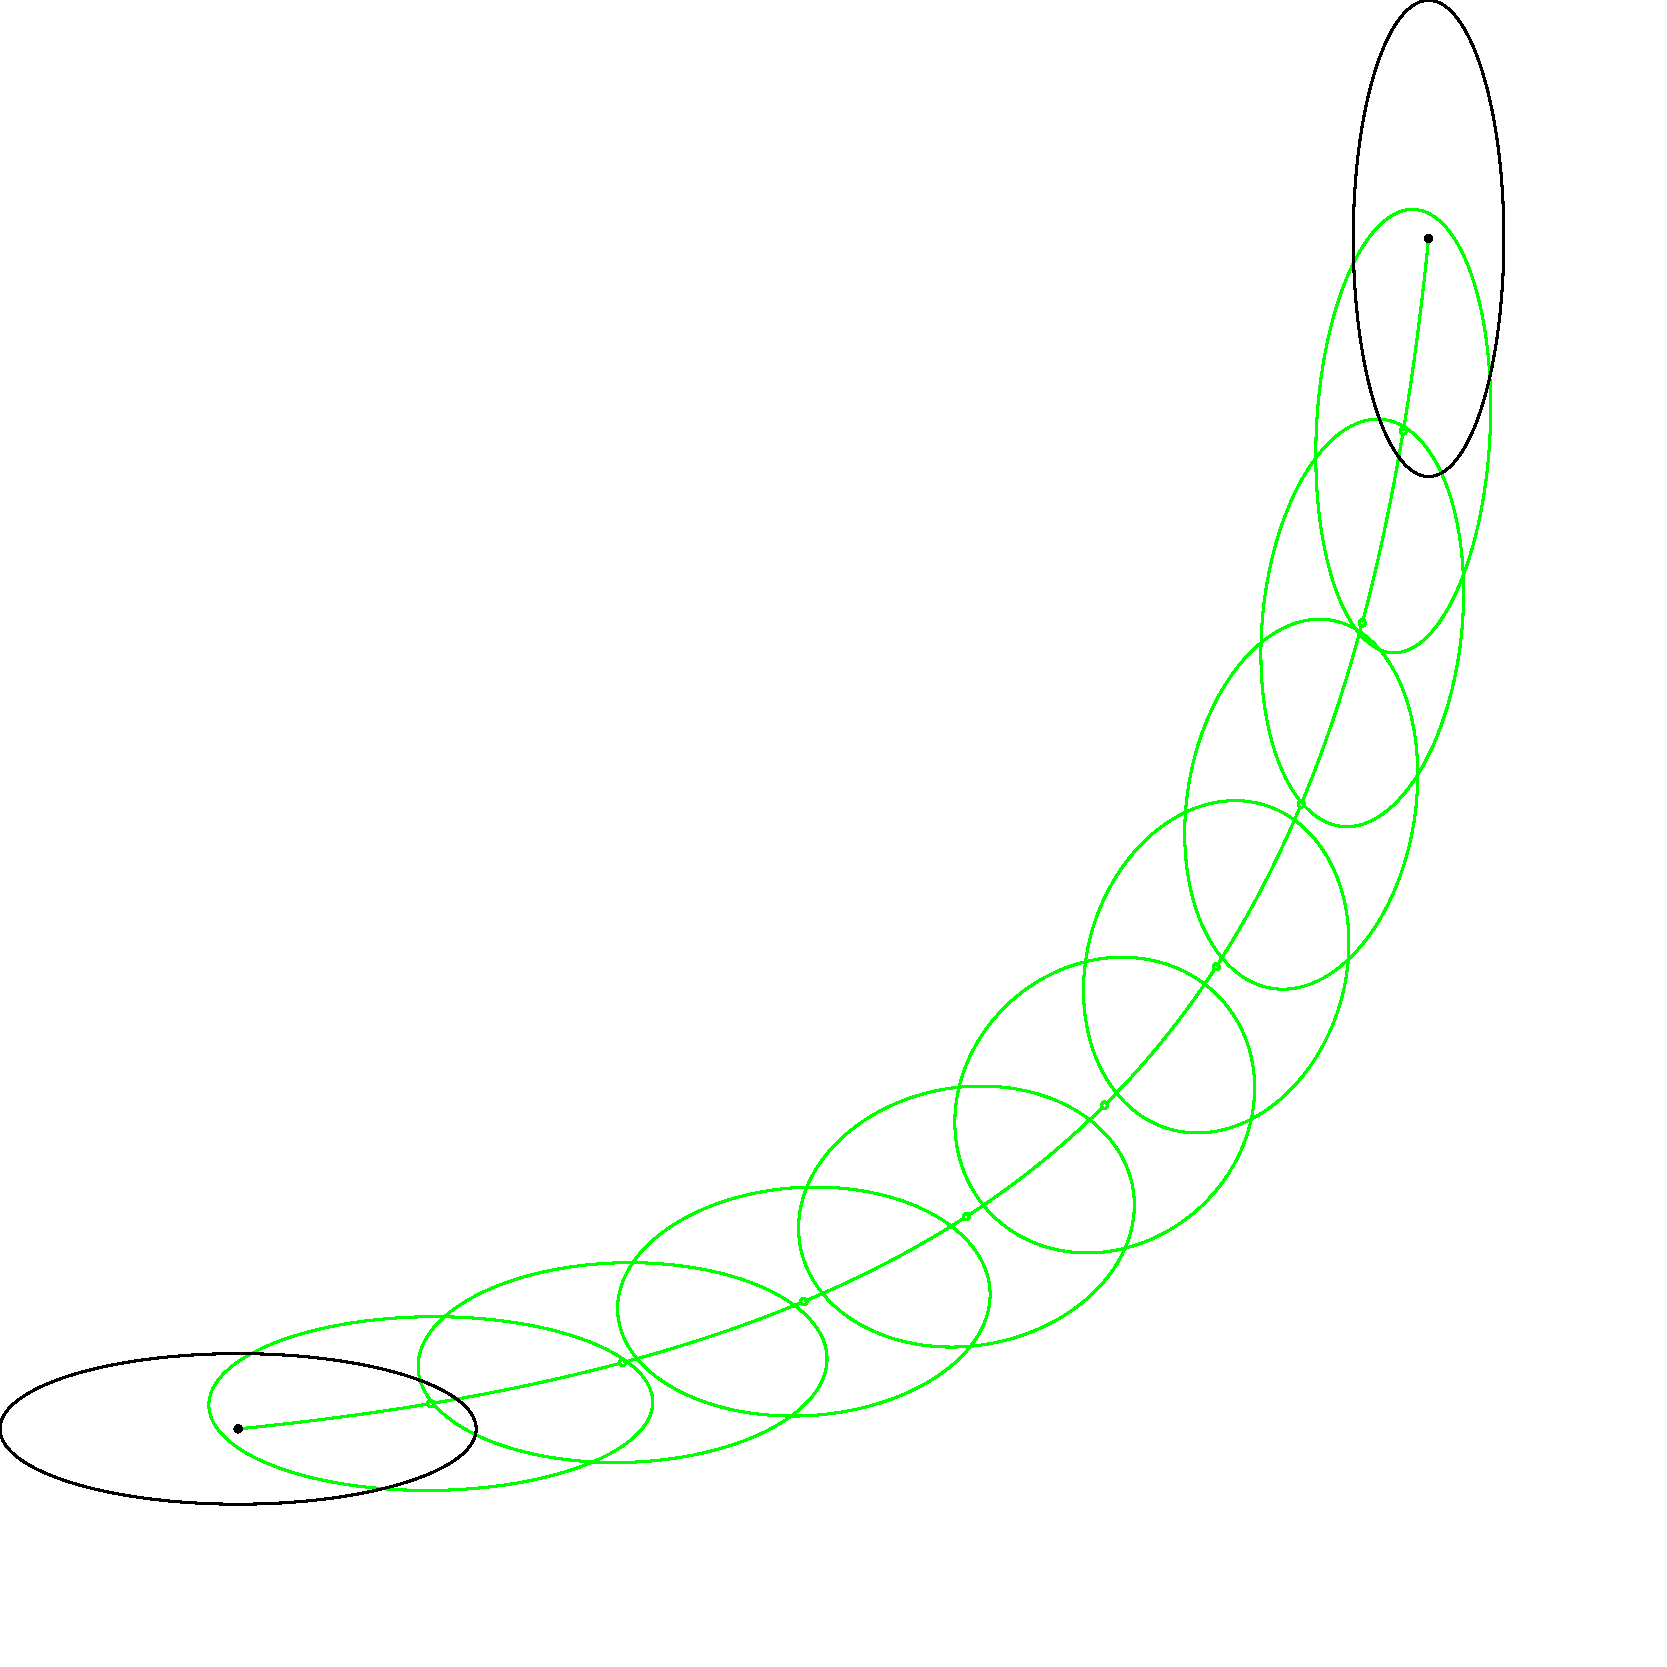
\includegraphics[width=0.25\textwidth]{BivariateNormal-52740-CO.pdf} \\
(\textbf{c}) mid-exp/mix curve & (\textbf{d}) projected C\&O curve \\
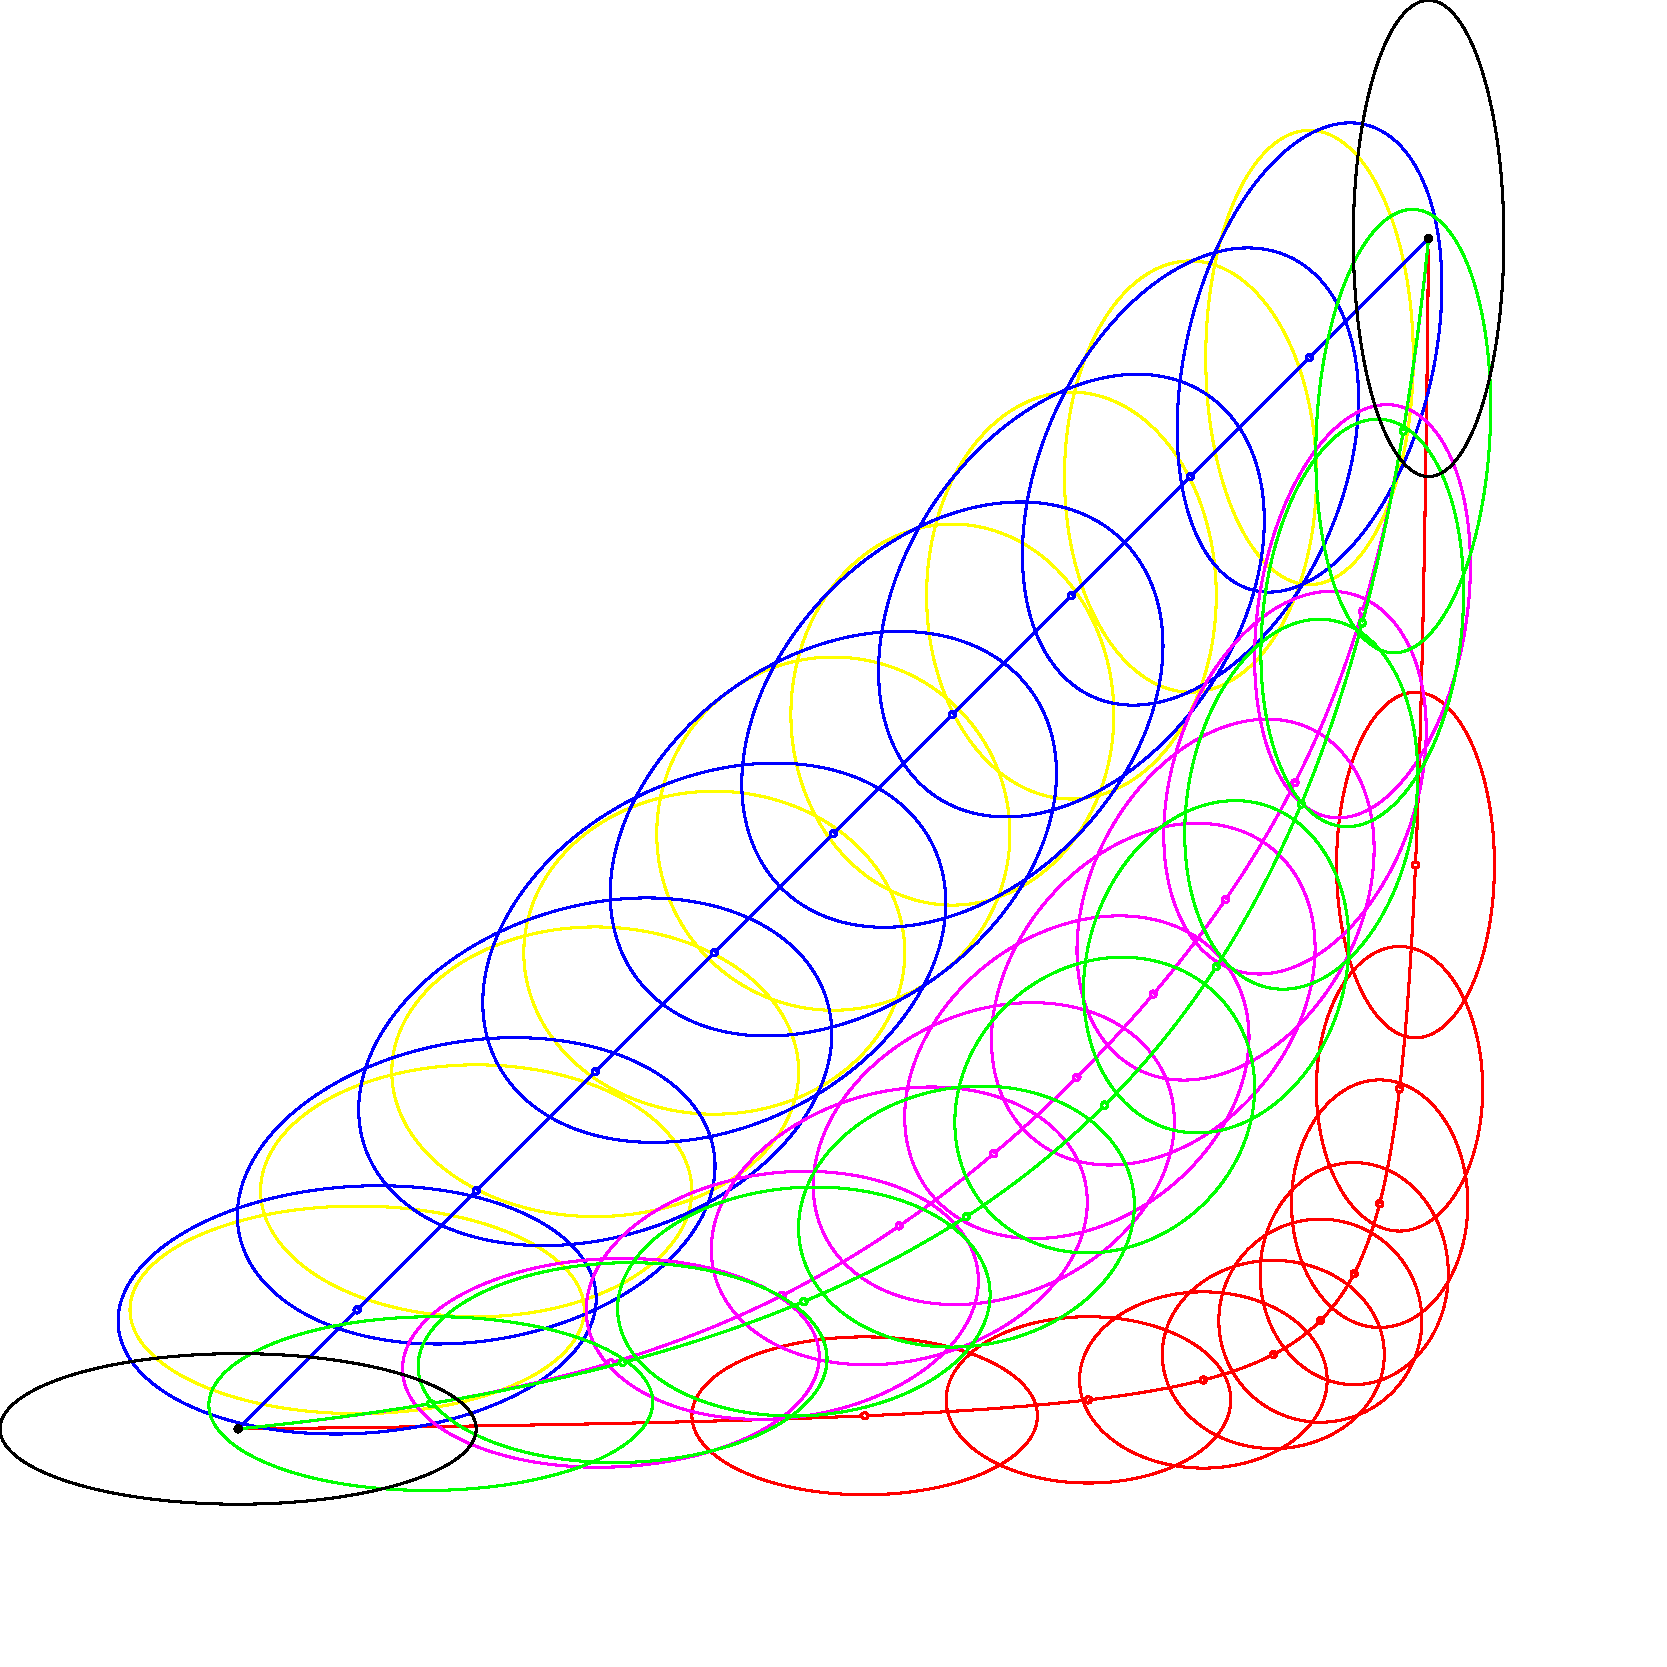
\includegraphics[width=0.25\textwidth]{BivariateNormal-52740-A.pdf} &
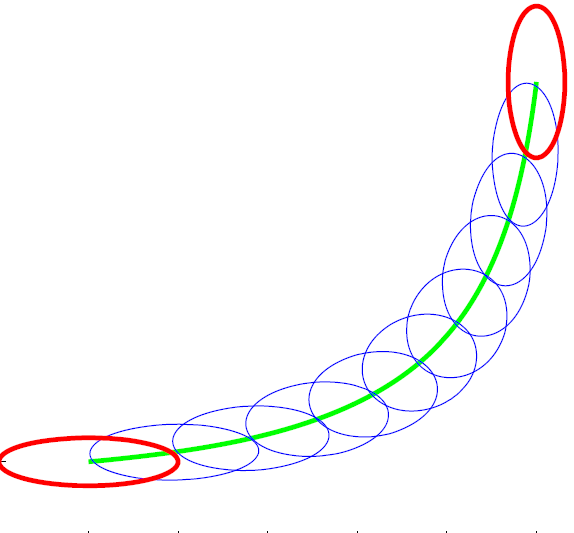
\includegraphics[width=0.25\textwidth]{HanPark-Fig5.png} \\
(\textbf{e}) geodesics/curves superposed & (\textbf{f}) Fisher--Rao {geodesic}
\end{tabular}
\caption{Comparison of our approximation curves with the Fisher--Rao geodesic (\textbf{f}) obtained by geodesic shooting (Figure~5 of~\cite{MVNGeodesicShooting-2014}). 
Exponential (\textbf{a}) and mixture (\textbf{b}) geodesics with the mid-exponential-mixture curve (\textbf{c}), and~the projected C\&O curve (\textbf{d}).
Superposed curves (\textbf{e}) and comparison with geodesic shooting (Figure~5 of~\cite{MVNGeodesicShooting-2014}).
Beware that color coding is not related between (\textbf{a}) and (\textbf{f}), and~scale for depicting ellipsoids are different.}\label{Fig:HanPark}
\end{figure}
\unskip

\begin{figure}[H]

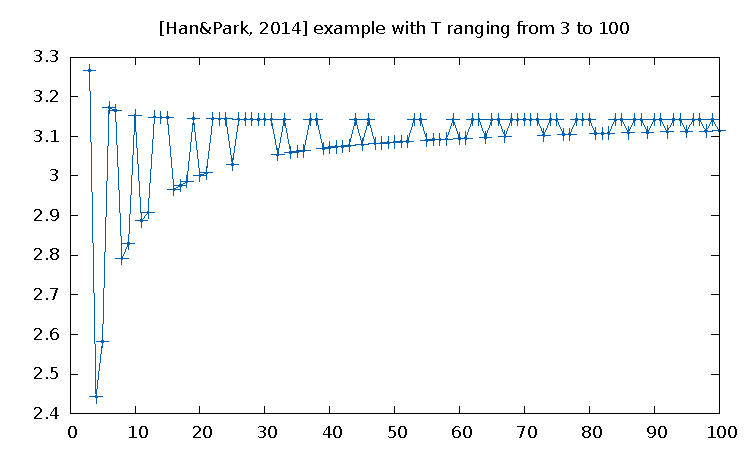
\includegraphics[width=0.85\textwidth]{HanParkPrecision3-100.pdf} 
\caption{Approximation of the Fisher–Rao distance obtained using the projected C\&O curve when $T$ ranges from $3$ to $100$.}
\label{Fig:HanParkRangeT}
\end{figure}
 
%Lower bound (Calvo and Oller):3.047019289671129
%Upper bound (S):5.430158841521429
%Upper bound (sqrt Jeffreys):4.3703546427569115
%LERP lambda:3.4495921895006005
%LERP eta:3.5774588585295612
%LERP theta:3.7314347818649316
%mid LERP theta-eta:3.167237545739778
%projected SPD geodesic:3.139052848069139



\item Bivariate normal $N_1=(0,I)$ and bivariate normal $N_2=(\mu_2,\Sigma_2)$ with $\mu_2=[1\ 0]^\top$ and 
$\Sigma_2=\mattwotwo{1}{-1}{-1}{2}$.
We obtain
\begin{itemize}
	\item Calvo and Oller lower bound: {\bf $1.4498$}
	\item Upper bound of Equation~(\ref{prop:USPC}): $2.6072$
	\item $\sqrt{D_J}$ upper bound: {\bf $1.5811$}
	\item $\tilde\rho^\lambda$: $1.5068$
	\item $\tilde\rho^m$: $1.5320$
	\item $\tilde\rho^e$: $1.5456$
	\item $\tilde\rho^{\mathrm{em}}$: $1.4681$
	\item $\tilde\rho^{\mathrm{co}}$: {\bf $1.4673$}
\end{itemize}
 \item Bivariate normal $N_1=(0,I)$ and bivariate normal $N_2=(\mu_2,\Sigma_2)$ with $\mu_2=[5\ 0]^\top$ and 
$\Sigma_2=\mattwotwo{1}{-1}{-1}{2}$.
We~get:
\begin{itemize}
	\item Calvo and Oller lower bound: {\bf $3.6852$}
	\item Upper bound of Equation~(\ref{prop:USPC}): {\bf $6.0392$}
	\item $\sqrt{D_J}$ upper bound: $6.2048$
	\item $\tilde\rho^\lambda$: $5.7319$
	\item $\tilde\rho^m$: $4.4039$
	\item $\tilde\rho^e$: $5.9205$
	\item $\tilde\rho^{\mathrm{em}}$: {\bf $4.2901$}
	\item $\tilde\rho^{\mathrm{co}}$: {$4.3786$}
\end{itemize}
\end{itemize}
\end{Example}

%Lower bound (Calvo and Oller):1.4497650597563339
%Upper bound (S):2.607215003535079
%Upper bound (sqrt Jeffreys):1.5811388300841898
%LERP lambda:1.5068752213920371
%LERP eta:1.5320371447524042
%LERP theta:1.545622344394067
%mid LERP theta-eta:1.468137744168569
%projected SPD geodesic:1.4673495361676057


%Lower bound (Calvo and Oller):3.6851723175926403
%Upper bound (S):6.03920329359525
%Upper bound (sqrt Jeffreys):6.2048368229954285
%LERP lambda:5.731978250975329
%LERP eta:4.403942256279602
%LERP theta:5.920585589635801
%mid LERP theta-eta:4.290099954605462
%projected SPD geodesic:4.378609296508541

See supplementary materials for further experiments.




%%%
\section{Approximating the Smallest Enclosing Fisher–Rao Ball of~MVNs}\label{sec:MEBMVN}   
%%%

We may use these closed-form distance $\rho_\CO(N,N')$ between $N$ and $N'$ 
to compute an approximation (of the center) of the smallest enclosing Fisher–Rao ball $B^*=\ball(C^*,r^*)$ of a set 
$\calG=\{N_1=(\mu_1,\Sigma_1),\ldots,N_n=(\mu_n,\Sigma_n)\}$ of $n$ $d$-variate normal distributions:
$$
C^*=\arg\min_{C\in\calN} \max_{i\in\{1,\ldots,n\}} \rho_\calN(C,N_i)
$$
where $\ball(C,r)=\{N\in\calN\st \rho_\calN(C,N)\leq r\}$.


The method proceeds as~follows:  
\begin{itemize}
\item First, we convert MVN set $\calG$ into the equivalent set of $(d+1)$-dimensional SPD matrices $\bar\calG=\{\barP_i=f(N_i)\}$ using the C\&O embedding. We relax the problem of approximating the circumcenter $C^*$ of the smallest enclosing Fisher–Rao ball by
$$
P^*=\arg\min_{P\in\bbP(d+1)} \max_{i\in\{1,\ldots,n\}} \rho_\CO(P,\barP_i).
$$

\item Second, we approximate the center of the smallest enclosing Riemannian ball of $\bar\calG$ using the iterative smallest enclosing Riemannian ball algorithm in~\cite{RieMinimax-2013} with say $T=1000$ iterations. 
Let $\tilde{P}\in\bbP(d+1)$ denote this approximation center: ${P}_T=\RieSEB_\SPD(\bar\calG,T)$.

\item Finally, we project back $P_T$ onto $\barN$: $\bar P_T=\proj_{\barN}({P}_T)$. 
We return $\bar P_T$ as the approximation of $C^*$.
\end{itemize}

Algorithm~\cite{RieMinimax-2013} $\RieSEB_\SPD(\{P_1,\ldots, P_n\},T)$ is described for a set of SPD matrices $\{P_1,\ldots, P_n\}$ as follows:

\begin{itemize}
	\item Let $C_1\leftarrow P_1$
	\item For $t=1$ to $T$
	\begin{itemize}
		\item Compute the index of the SPD matrix which is farthest from the current circumcenter $C_t$:
		$$
		f_t=\arg\max_{i\in\{1,\ldots,n\}} \rho_\SPD(C_t,P_i)
		$$
		\item Update the circumcenter by walking along the geodesic linking $C_t$ to $P_{f_t}$:
		$$
		C_{t+1}=\gamma_\SPD\left(C_t,P_{f_t};\frac{1}{t+1}\right)
		= C_t^{\frac{1}{2}}(C_t^{-\frac{1}{2}}P_{f_t}C_t^{-\frac{1}{2}})^{\frac{1}{t+1}} C_t^{\frac{1}{2}}
		$$
	\end{itemize}
	\item Return $C_T$
\end{itemize}

The convergence of the algorithm $\RieSEB_\SPD$ follows from the fact that the SPD trace manifold is a Hadamard manifold (with negative sectional curvatures). See~\cite{RieMinimax-2013} for proof of~convergence.

The SPD distance $\rho_\calP(C_T,\bar C_T)$ indicates the quality of the approximation.
Figure~\ref{fig:MiniBallCO} shows the result of implementing this~heuristic.

Let us notice that when all MVNs share the same covariance matrix $\Sigma$, we have from Equation~(\ref{eq:FRsamecovar}) or Equation~(\ref{eq:cosamecovar}) 
that $\rho_\calN(\mu_1,\Sigma),N(\mu_2,\Sigma)$ and $\rho_{\CO}(N(\mu_1,\Sigma),N(\mu_2,\Sigma))$ are strictly increasing function of their Mahalanobis distance.
Using the Cholesky decomposition $\Sigma^{-1}=LL^\top$, we deduce that the smallest Fisher–Rao enclosing ball coincides with the
smallest Calvo and Oller enclosing ball, and~ the  circumcenter of that ball can be found  as an ordinary Euclidean circumcenter~\cite{welzl2005smallest} 
(Figure~\ref{fig:MiniBallCO}b).
Please note that in 1D, we can find the exact smallest enclosing Fisher–Rao ball as an equivalent smallest enclosing ball in hyperbolic~geometry.
 

Furthermore, we may extend the computation of the approximated circumcenter to  $k$-center clustering~\cite{gonzalez1985clustering} of $n$ multivariate normal distributions. Since the circumcenter of the clusters is approximated and not exact, we extend straightforwardly the variational approach of $k$-means described in~\cite{acharyya2013bregman} to $k$-center clustering.
An application of $k$-center clustering of MVNs is to simplify a Gaussian mixture model~\cite{FRMVNReview-2020} (GMM).



Similarly, we can consider other Riemannian distances with closed-form formulas between MVNs such as the Killing distance in the symmetric space~\cite{lovric2000multivariate} (see Appendix~\ref{sec:SS}) or the Siegel-based distance proposed in Appendix~\ref{sec:Siegel}.

\begin{figure}[H]

\begin{tabular}{ccc}
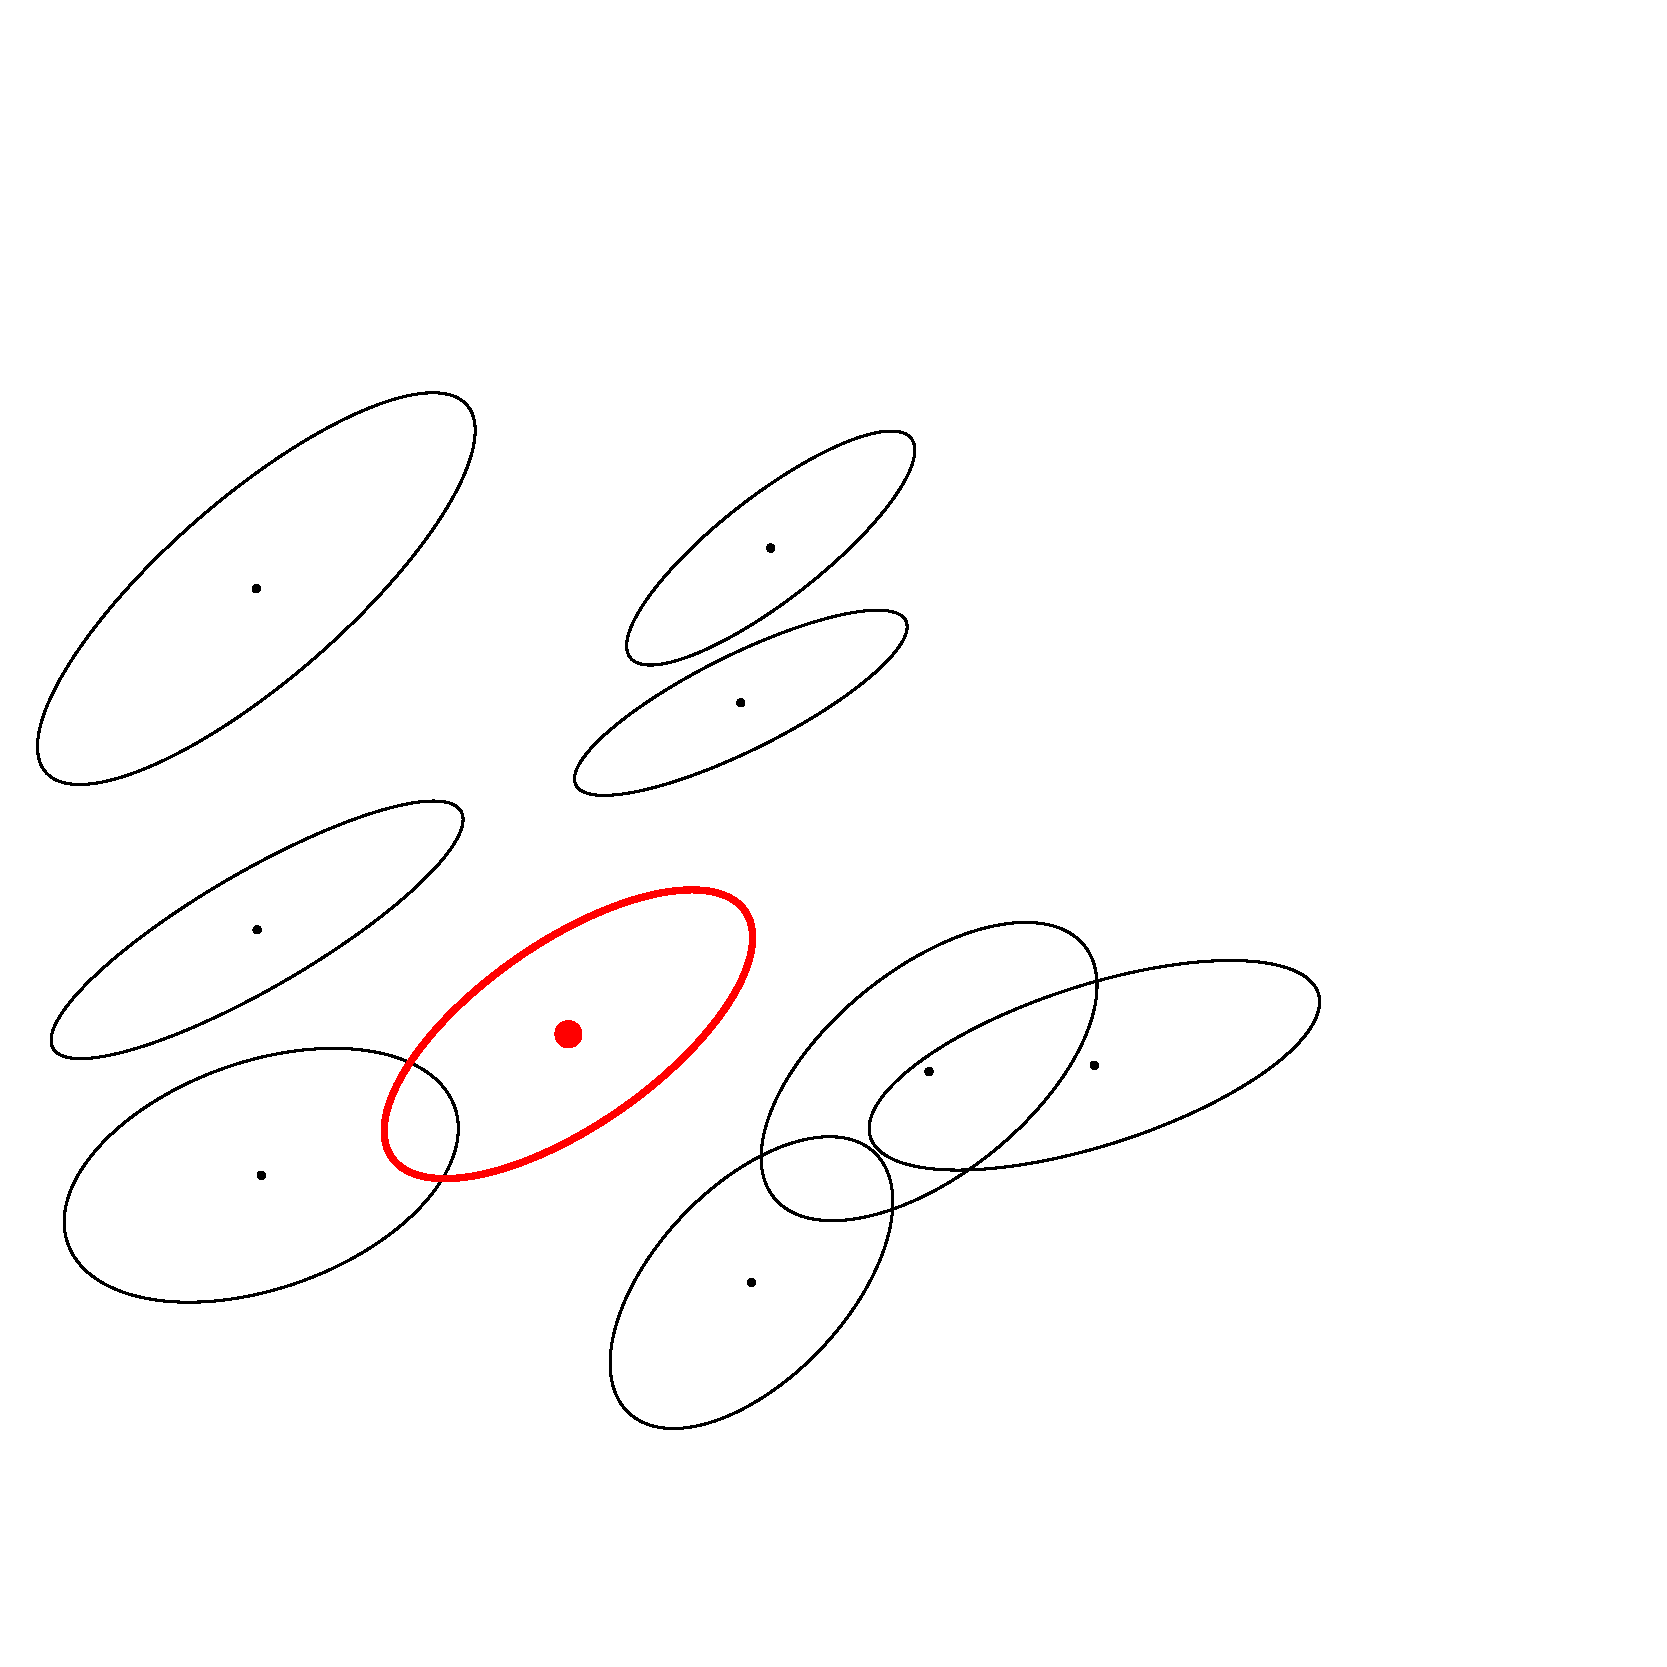
\includegraphics[width=0.25\textwidth]{MiniMaxCenterMVN-N8.pdf} &
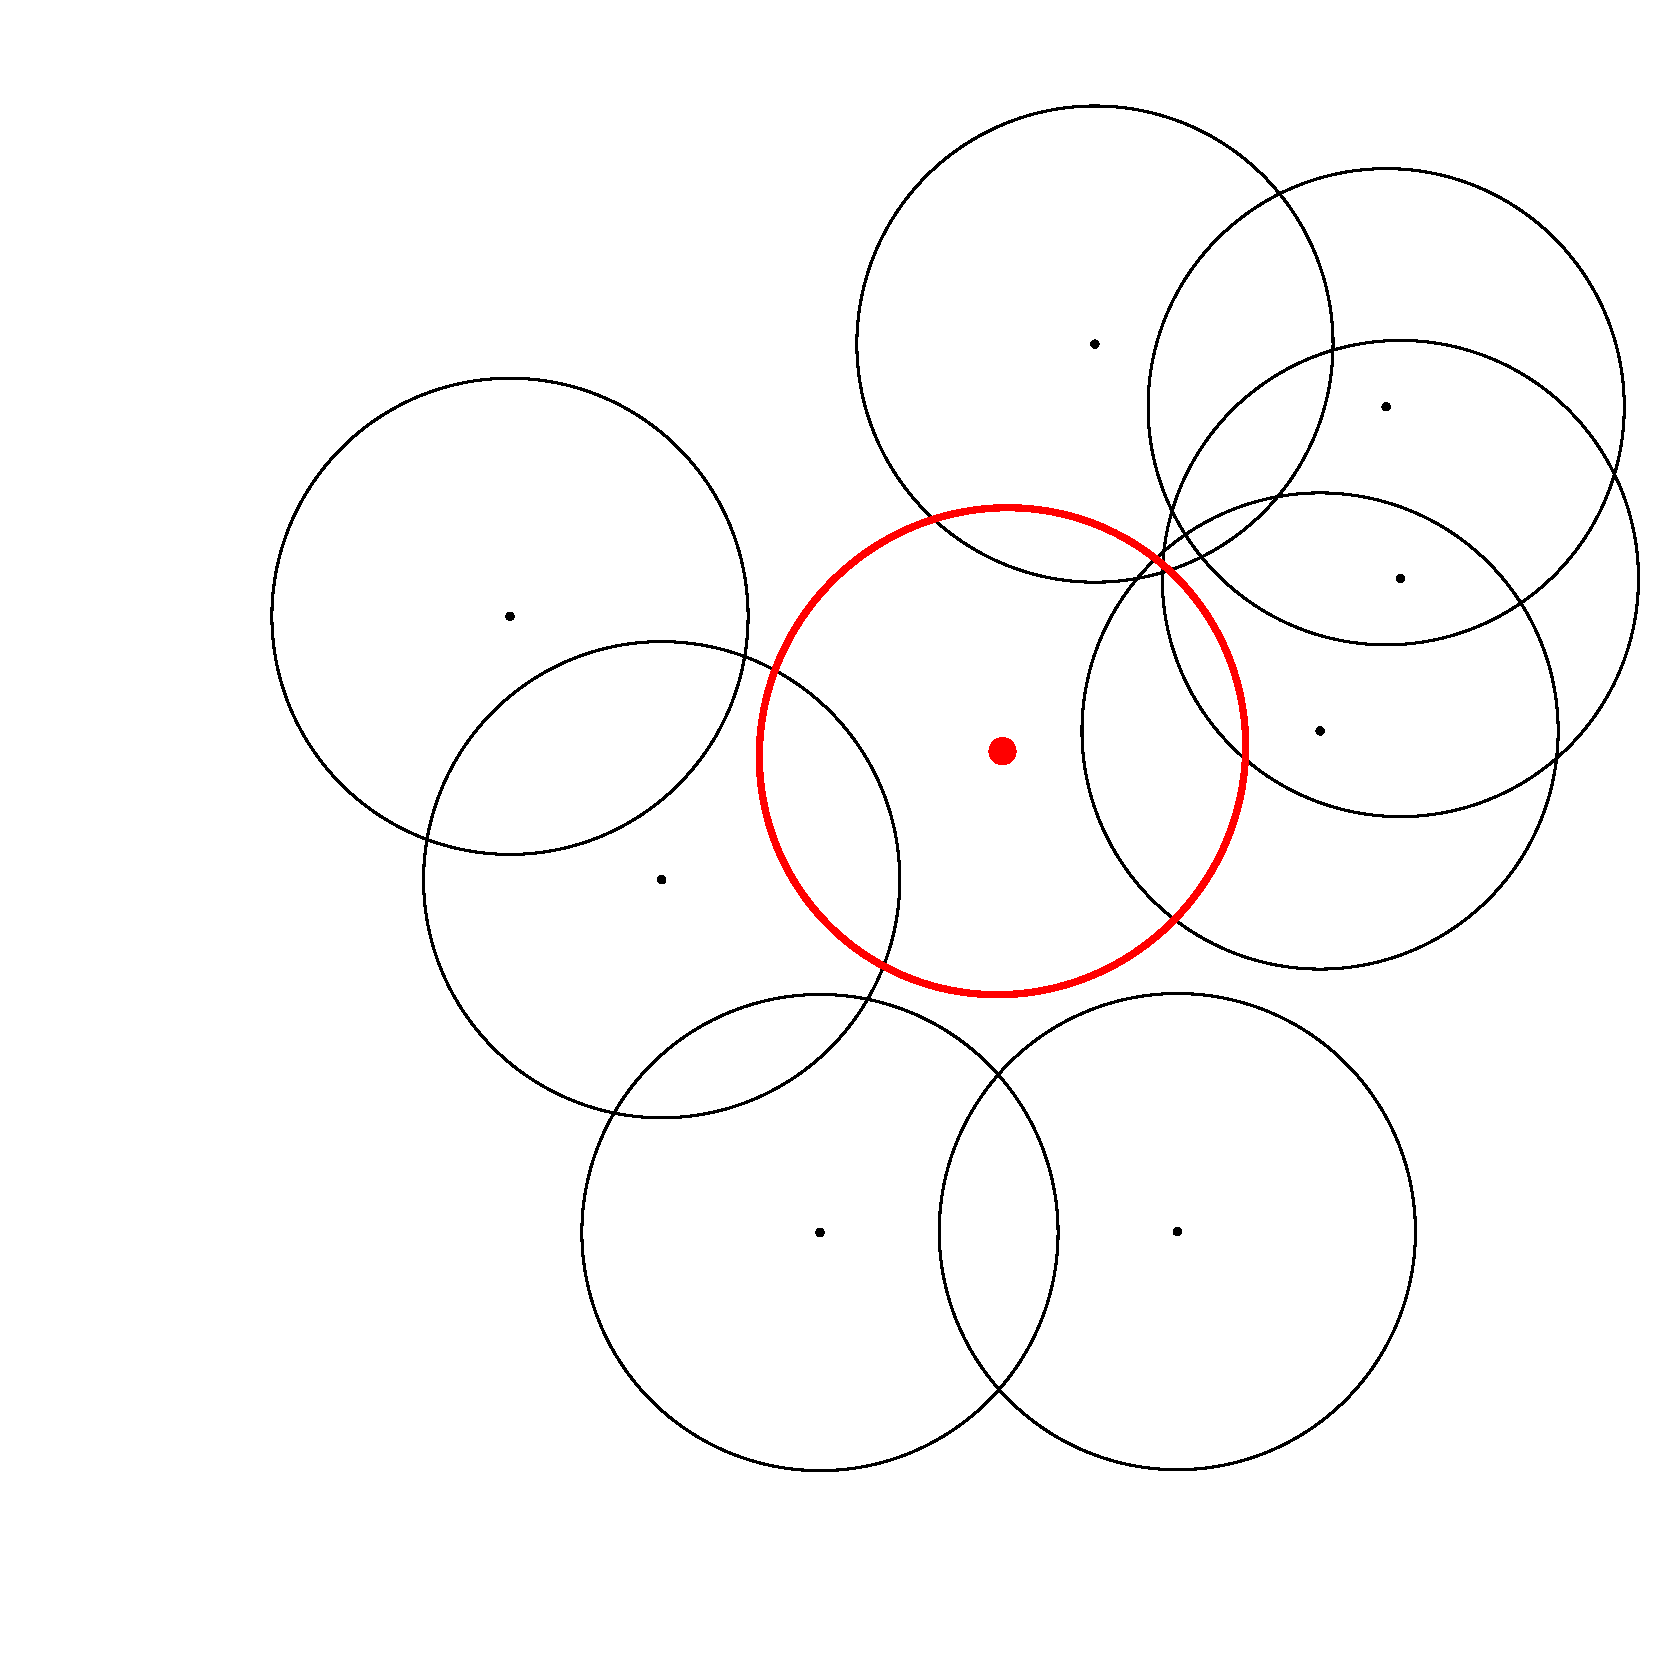
\includegraphics[width=0.25\textwidth]{MiniMaxCenterMVN-SameCovarN8.pdf} &
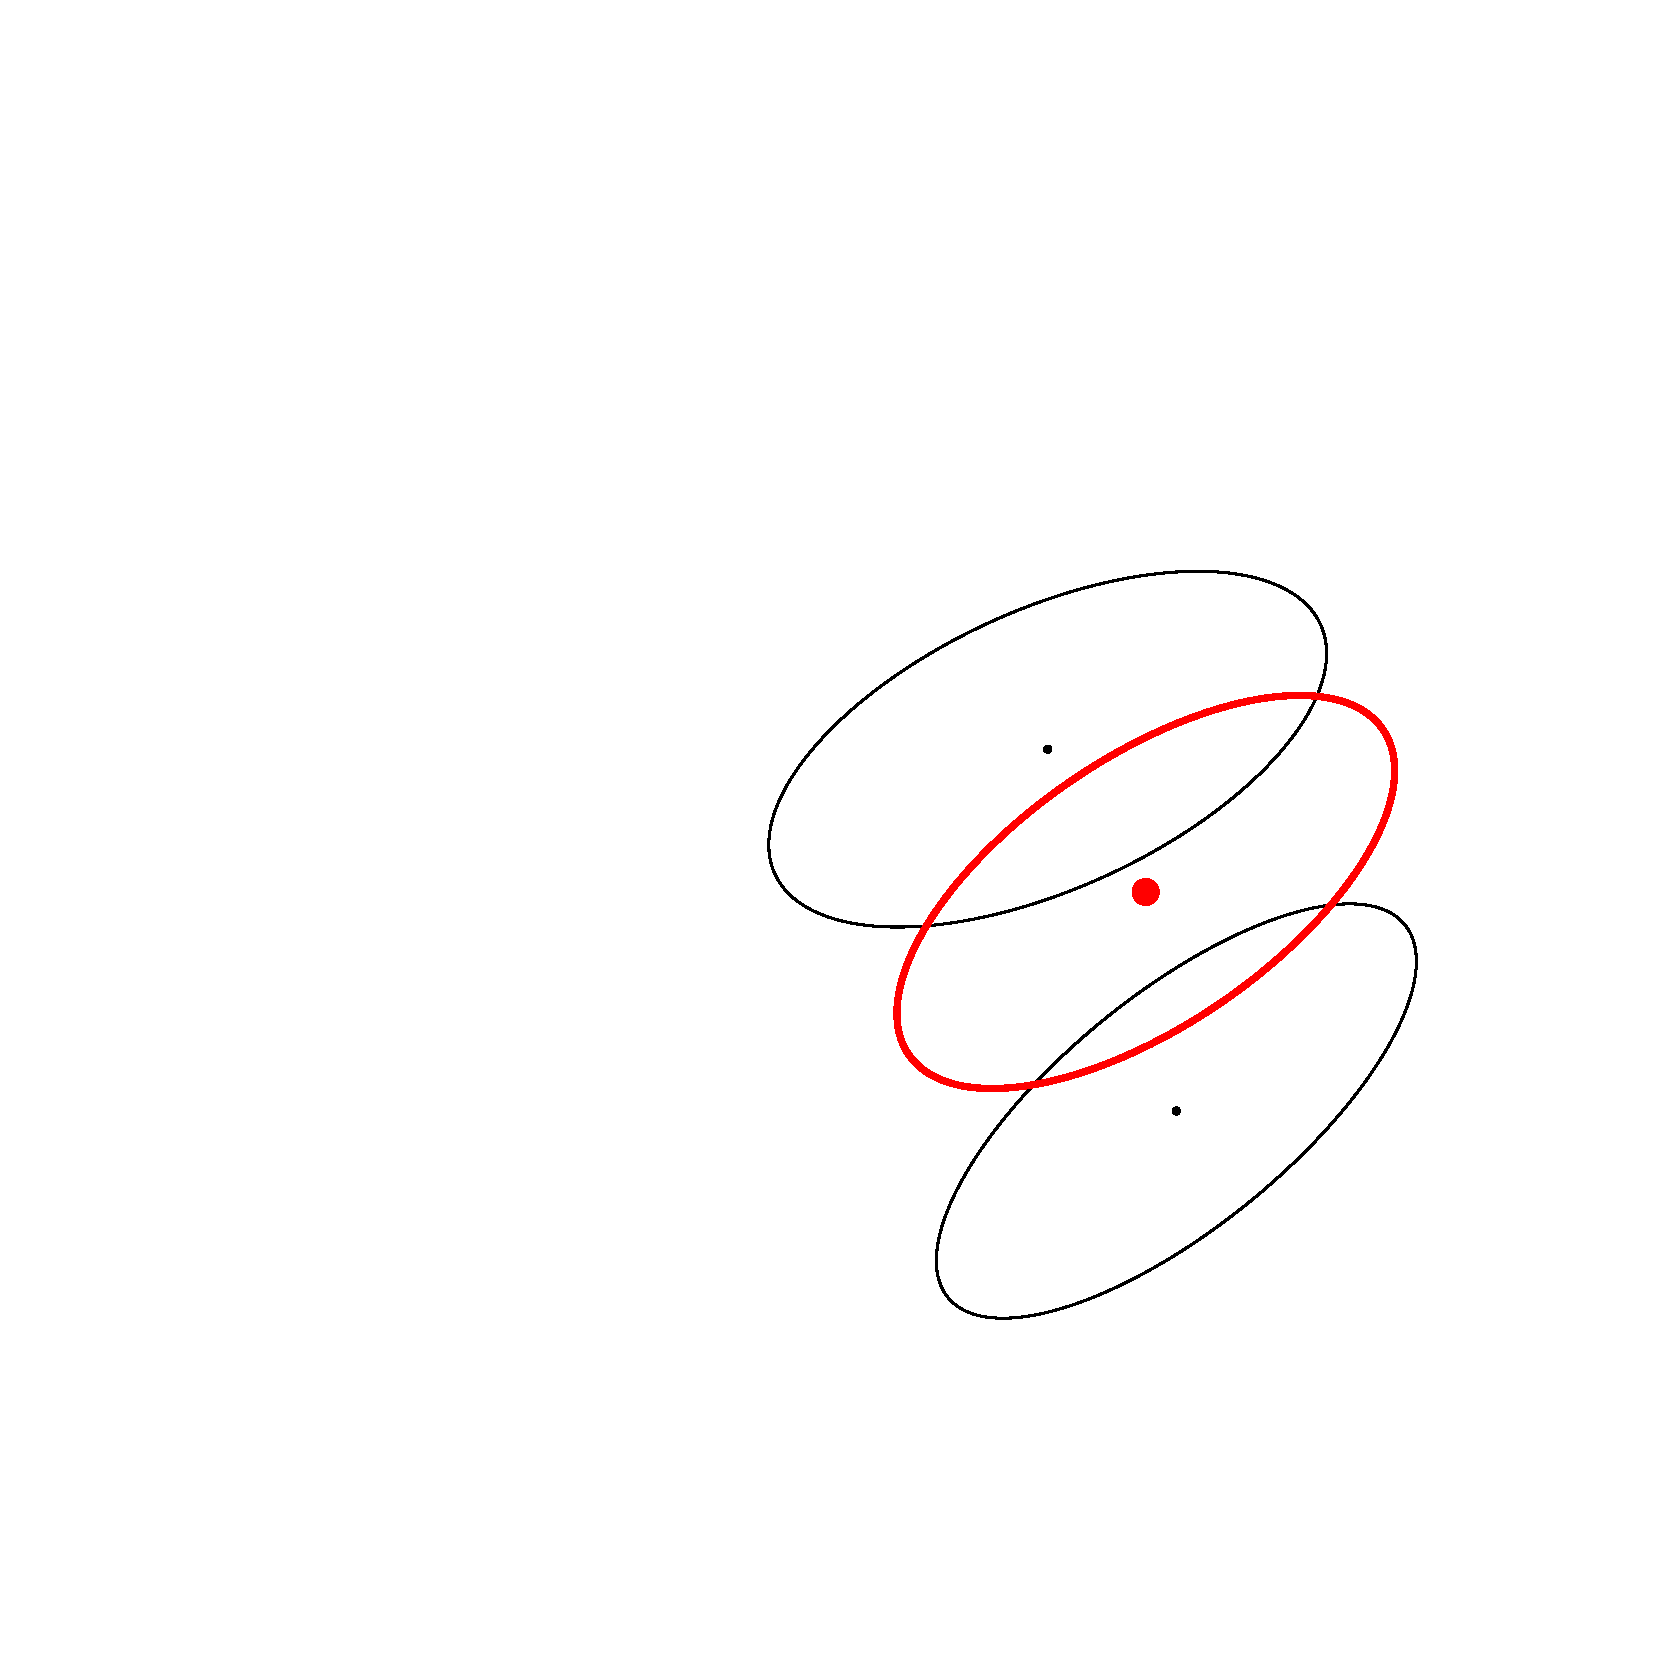
\includegraphics[width=0.25\textwidth]{MiniMaxCenterMVN-N2.pdf}\\
(\textbf{a}) & (\textbf{b}) & (\textbf{c})
\end{tabular}


\caption{Approximation of the smallest enclosing Riemannian ball of a set of $n$ bivariate normals $N_i=N(\mu_i,\Sigma_i)$ with respect to C\&O distance $\rho_\CO$ (the approximate circumcenter $\bar C_T$ is depicted as a red ellipse):
(\textbf{a}) $n=8$ with different covariance matrices,
(\textbf{b}) $n=8$ with identical covariance matrices amount to the smallest enclosing ball of a set of $n$ points $\{\mu_i\}$,
(\textbf{c}) $n=2$ displays the midpoint of the C\&O geodesic visualized as an equivalent bivariate normal distribution in the sample space.
 \label{fig:MiniBallCO}}
\end{figure}
\unskip

%%%
\section{Some Information–Geometric Properties of the C\&O~Embedding}\label{sec:prop}  %  Calvo \& Oller 
%%%

In information geometry~\cite{IG-2016}, the~manifold $\calN$ admits a dual structure denoted by the quadruple 
$$
(\calN,g^\Fisher_\calN,\nabla^e_\calN,\nabla^m_\calN),
$$ 
when equipped with the exponential connection $\nabla^e_\calN$ and the mixture connection $\nabla^m_\calN$. 
The connections $\nabla^e_\calN$ and $\nabla^m_\calN$ are said to be dual since $\frac{\nabla^e_\calN+\nabla^m_\calN}{2}=\bar\nabla_\calN$, the Levi–Civita connection induced by $g^\Fisher_\calN$.
Furthermore, by~viewing $\calN$ as an exponential family $\{p_\theta\}$ with natural parameter $\theta=(\theta_v,\theta_M)$ (using the sufficient statistics~\cite{nielsen2019jensen} $(x,-xx^\top)$), and~taking the convex log-normalizer function $F_\calN(\theta)$ of the normals, we can build a dually flat space~\cite{IG-2016} where the canonical divergence amounts to a Bregman divergence which coincides with the reverse Kullback–Leibler divergence~\cite{ohara1996dualistic,IG-MVN-1999} (KLD).
The Legendre duality 
$$
F^*(\eta)=\inner{\nabla F(\theta)}{\eta}-F(\nabla F(\theta))
$$
 \textls[-15]{(with $\inner{(v_1,M_1)}{(v_2,M_2)}=\tr(v_1v_2^\top+M_1M_2^\top)=v_1\cdot v_2+\tr(M_1M_2^\top)$) yields:
$\theta =  (\theta_v,\theta_M)\\=\left(\Sigma^{-1}\mu,\frac{1}{2}\Sigma^{-1}\right)$,}
$$
F_\calN(\theta) = \frac{1}{2}\left(d\log\pi-\log|\theta_M|+\frac{1}{2}\theta_v^\top\theta_M^{-1}\theta_v\right),$$
$\eta=(\eta_v,\eta_M)=\nabla F_\calN(\theta)=\left(\frac{1}{2}\theta_M^{-1}\theta_v,\theta_M^{-1}\right)$,
$$F^*_\calN(\eta)= -\frac{1}{2}\left(\log(1+\eta_v^\top\eta_M^{-1}\eta_v)+\log|-\eta_M|+d(\log 2\pi e)\right),$$
and we have
$$
B_{F_\calN}(\theta_1,\theta_2)=D_\KL^*(p_{\lambda_1}:p_{\lambda_2})=D_\KL(p_{\lambda_2}:p_{\lambda_1})=B_{F^*_\calN}(\eta_2:\eta_1),
$$
where $D_\KL^*[p:q]=D_\KL[q:p]$ is the reverse~KLD.

In a dually flat space, we can express the canonical divergence as a Fenchel–Young divergence using the mixed coordinate systems $
B_{F_\calN}(\theta_1:\theta_2)=Y_{F_\calN}(\theta_1:\eta_2)$
where $\eta_i=\nabla F_\calN(\theta_i)$ and 
$$
Y_{F_\calN}(\theta_1:\eta_2):=F_\calN(\theta_1)+F^*_\calN(\eta_2)-\inner{\theta_1}{\eta_2}.
$$
The  moment $\eta$-parameterization of a normal is $(\eta=\mu,H=-\Sigma-\mu\mu^\top)$
with its reciprocal function $(\lambda=\eta,\Lambda=-H-\eta\eta^\top)$.


Let $F_\calP(P)=F_\calN(0,P)$, $\bar\theta=\frac{1}{2}\bar P^{-1}$, $\bar\eta=\nabla F_{\calP}(\bar\theta)$. 
Then we have the following proposition which proves that the Fenchel–Young divergences in $\calN$ and $\barN$ (as a submanifold of $\calP$)  coincide:


\begin{Proposition}\label{prop:embedpot}
We have
\begin{eqnarray*}
D_\KL[p_{\mu_1,\Sigma_1}:p_{\mu_2,\Sigma_2}]&=&
B_{F_\calN}(\theta_2:\theta_1)=Y_{F_\calN}(\theta_2:\eta_1)
=Y_{F_\calP}(\bar\theta_2:\bar\eta_1)\\
&=& 
B_{F_\calP}(\bar\theta_2:\bar\theta_1)=
D_\KL[p_{0,\bar P_1=f(\mu_1,\Sigma_2)}:p_{0,\bar P_2=f(\mu_2,\Sigma_2)}].
\end{eqnarray*}
\end{Proposition}


Consider now the $\nabla^e$-geodesics and $\nabla^m$-geodesics on $\calN$ (linear interpolation with respect to natural and dual moment parameterizations, respectively):
$\gamma_\calN^e(N_1,N_2;t)=(\mu_t^e,\Sigma_t^e)$ and
$\gamma_\calN^m(N_1,N_2;t)=(\mu_t^m,\Sigma_t^m)$.

\begin{Proposition}[Mixture geodesics preserved]\label{prop:geo}
The mixture geodesics are preserved by the embedding $f$: 
$f(\gamma_\calN^m(N_1,N_2;t))=\gamma_\calP^m(f(N_1),f(N_2);t)$.
The exponential geodesics are preserved for the subspace of $\calN$ with fixed mean $\mu$: $\calN_\mu$.
\end{Proposition}

\begin{proof}
For the $m$-geodesics, let us check that 
$$
f(\mu_t^m,\Sigma_t^m)=
\mattwotwo{\Sigma_t^m+\mu_t^m{\mu_t^m}^\top}{\mu_t^m}{(\mu_t^m)^\top}{1}=
t \underbrace{f(\mu_1,\Sigma_1)}_{\bar P_1}+(1-t)\underbrace{f(\mu_2,\Sigma_2)}_{\barP_2},
$$
\textls[-25]{since $\Sigma_t^m+\mu_t{\mu_t^m}^\top=
\bar\Sigma_t+t\mu_1\mu_1^\top+(1-t)\mu_2\mu_2^\top$ $= t (\Sigma_1+\mu_1\mu_1^\top)+(1-t)(\Sigma_2+\mu_2\mu_2^\top)$.}
Thus, we have $f(\gamma_\calN^m(N_1,N_2;t))=\gamma_\calP^m(\bar P_1,\bar P_2;t)$.
\end{proof}
 
 
Therefore, all algorithms on $\calN$ which only require $m$-geodesics or $m$-projections~\cite{IG-2016} by minimizing the right-hand side of the KLD can be implemented by algorithms on $\calP$. See, for example, the~minimum enclosing ball approximation algorithm called BBC in~\cite{BBC-2005}. 
Notice that $\barN_\mu$ (fixed mean normal submanifolds) preserve both mixture and exponential geodesics: 
The submanifolds $\barN_\mu$ are said to be doubly autoparallel~\cite{ohara2019doubly}.

\begin{Remark}
In~\cite{calin2014geometric} (p. 355), exercises 13.8 and 13.9 ask to prove the equivalence of the following statements for $\calS$ a submanifold of $\calM$:
\begin{itemize}
	\item $\calS$ is an exponential family $\Leftrightarrow$ $\calS$ is $\nabla^1$-autoparallel in $\calM$ (exercise 13.8),
	\item $\calS$ is a mixture family $\Leftrightarrow$ $\calS$ is $\nabla^{-1}$-autoparallel in $\calM$ (exercise 13.9).
\end{itemize}
  
\textls[-15]{Let ${\bar P}=\mattwotwo{\Sigma+\mu\mu^\top}{\mu}{\mu^\top}{1}$ (with $|{\bar P}|=|\Sigma|$),
$
{\bar P}^{-1}=
\mattwotwo{\Sigma^{-1}}{-\Sigma^{-1}\mu}{-\mu^\top\Sigma^{-1}}{1+\mu^\top \Sigma^{-1}\mu}$, and~$y=(x,1)$.
Then we have}
\begin{eqnarray*}
q_{\bar P}(y) &=& \frac{1}{(2\pi)^\frac{d+1}{2} \sqrt{|\bar P|}} \exp\left(-\frac{1}{2}y^\top \bar P^{-1} y\right),\\
 &=& \frac{1}{(2\pi)^\frac{d+1}{2} \sqrt{|\Sigma|}} \exp\left(-\frac{1}{2}y^\top \bar P^{-1} y\right),\\
&=& \frac{1}{(2\pi)^\frac{d+1}{2} \sqrt{|\Sigma|}} \exp\left([x^\top\ 1] \mattwotwo{\Sigma^{-1}}{-\Sigma^{-1}\mu}{-\mu^\top\Sigma^{-1}}{1+\mu^\top \Sigma^{-1}\mu} \vectortwo{x}{1}\right).
\end{eqnarray*}
Thus, $\barN=\{q_{\bar P}(x,1)\}$ is an exponential family.
Therefore, we deduce that $\calP$ is $\nabla^e$-autoparallel in $\calP$.
However, $\barN$ is not a mixture family and thus $\calP$ is not $\nabla^{m}$-autoparallel in $\calP$.
\end{Remark}



%%%
\section{Conclusions and~Discussion}\label{sec:concl}
%%%

In general, the~Fisher--Rao distance between multivariate normals (MVNs) is not known in closed form.
In practice, the~Fisher--Rao distance is usually approximated by costly geodesic shooting techniques~\cite{MVNGeodesicShooting-2014,GeodesicShooting-2016,barbaresco2019souriau}  which requires time-consuming computations of the Riemannian exponential map and are nevertheless limited to normals within a short range of each other. 
In this work, we consider a simple alternative approach for approximating the Fisher--Rao distance by approximating the Riemannian lengths of curves, which admits closed-form parameterizations. 
In particular, we considered the mixed exponential-mixture curved and the projected symmetric positive–definite matrix geodesic obtained from Calvo and Oller isometric submanifold embedding into the SPD cone~\cite{SDPMVN-1990}.
We summarize our method to approximate $\rho_\calN(N_1,N_2)$ between $N_1=N(\mu_1,\Sigma_1)$ and $N_2=N(\mu_2,\Sigma_2)$ as follows:
$$
\tilde\rho_T^\CO(N_1,N_2) := 
\frac{1}{T} \sum_{i=1}^{T-1} \sqrt{D_J\left[\barS_t,\barS_{t+1}\right]},
$$
where 
$$
\barS_t=\proj_{\barN}\left(S_t)\right),\quad  
\proj_{\barN}\left(\mattwotwo{\Sigma+\beta\mu\mu^\top}{\beta\mu}{\beta\mu^\top}{\beta}\right)=\mattwotwo{\Sigma+\mu\mu^\top}{\mu^\top}{\mu}{1}
$$
and
$$
S_t=\barP_1^{\frac{1}{2}} \, \left(\barP_1^{-\frac{1}{2}}\barP_2^{\frac{1}{2}}\barP_1^{-\frac{1}{2}}\right)^{\frac{t}{T}}
 \, \barP_1^{\frac{1}{2}}
$$
with 
$$
\barP_1=f(N_1)=\mattwotwo{\Sigma_1+\mu_1\mu_1^\top}{\mu_1}{\mu_1^\top}{1},\quad \barP_2=f(N_2)=\mattwotwo{\Sigma_2+\mu_2\mu_2^\top}{\mu_2}{\mu_2^\top}{1}.
$$
We proved the following sandwich bounds of our approximation
$$
\rho_\calN(N_1,N_2)\leq \tilde\rho_T^\CO(N_1,N_2) \leq  \rho_\calN(N_1,N_2) + 2 \delta^\CO_T(\bar P_1,\bar P_2),
$$
where
$$
\delta^\CO_T(P_1,P_2):=\frac{1}{T}\sum_{i=1}^T  \rho_\calP(S_t,\bar{S}_t).
$$
Notice that we may  calculate equivalently $D_J\left[\barS_t,\barS_{t+1}\right]$ as $D_J[G_t,G_{t+1}]$ where $G_i=f^{-1}(\barS_i)=N(m_i,C_i)$ for $i\in\{0,\ldots,T\}$ (see Proposition~\ref{prop:KL}).

We also reported a fast way to upper bound the Fisher--Rao distance by the square root of Jeffreys' divergence: $\rho_\calN(N_1,N_2)\leq \sqrt{D_J[N_1,N_2]}$ which is tight at infinitesimal scale.
In practice, this upper bound beats the upper bound of~\cite{strapasson2015bounds} when normal distributions are not too far from each other. 
Finally, we show that not only is
Calvo and Oller  SPD submanifold embedding~\cite{SDPMVN-1990} isometric, but~it also preserves the Kullback–Leibler divergence, the Fenchel–Young divergence, and the mixture geodesics. 
Our approximation technique extends to elliptical distribution, which generalizes multivariate normal distributions~\cite{SDPElliptical-2002,chen2022multisensor}.
Moreover, we obtained a closed form for the Fisher–Rao distance between normals sharing the same covariance matrix using the technique of maximal invariance under the action of the affine group in Section~\ref{sec:FRsamecovar}.
We may also consider other distances different from the Fisher--Rao distance, which admits a closed-form formula:
For example, the~Calvo and Oller metric distance~\cite{SDPMVN-1990} (a lower bound on the Fisher–Rao distance) or the metric distance proposed in~\cite{lovric2000multivariate} (see Appendix~\ref{sec:SS}) whose geodesics enjoys the asymptotic property of the Fisher--Rao geodesics~\cite{globke2021information}). 
The C\&O distance is very well-suited for short Fisher--Rao distances while the symmetric space distance is well-tailored for 
large Fisher–Rao distances. The~calculations of these closed-form distances rely on generalized eigenvalues.
We also propose an embedding of normals into the Siegel upper space in Appendix~\ref{sec:Siegel}.
To conclude, let us propose yet another alternative distance, The Hilbert projective distance on the SPD cone~\cite{nielsen2019clustering}, which only needs to calculate the minimal and maximal eigenvalues (say, using the power iteration method~\cite{journee2010generalized}):
\begin{equation}
\rho_\Hilbert(P_1,P_2)= \log\left(\frac{\lambda_{\mathrm{max}}(P_1^{-1}P_2)}{\lambda_{\mathrm{min}}(P_1^{-1}P_2)}\right).
\end{equation}
The dissimilarity is said projective on the SPD cone because $\rho_\Hilbert(P_1,P_2)=0$ if and only if $P_1=\lambda P_2$ for some $\lambda>0$.
However, let us notice that it yields a proper metric distance on $\barN$:
$$
\rho_\Hilbert(N_1,N_2):=\rho_\Hilbert(\barP_1,\barP_2),
$$
since $\barP_1=\lambda\barP_2$ if and only if $\lambda=1$ because the array element $(P_1)_{d+1,d+1}=(P_2)_{d+1,d+1}=1$, i.e.,~$\barP_1=\barP_2$ implying  $P_1=P_2$ by the isometric diffeomorphism $f$.

Notice that since $\lambda_{\mathrm{max}}(P)=\lambda_{\mathrm{min}}(P^{-1})$,
$\lambda_{\mathrm{min}}(P)=\lambda_{\mathrm{max}}(P^{-1})$, \\
$\lambda_{\mathrm{max}}(P_1P_2)\leq \lambda_{\mathrm{max}}(P_1)\lambda_{\mathrm{max}}(P_2)$, and~
$\lambda_{\mathrm{min}}(P_1P_2)\geq \lambda_{\mathrm{min}}(P_1)\lambda_{\mathrm{min}}(P_2)$, we have the following upper bound on Hilbert distance: 
$\rho_\Hilbert(P_1,P_2)\leq \log\frac{\lambda_{\mathrm{max}}(P_1)}{\lambda_{\mathrm{min}}(P_1)}+
\log\frac{\lambda_{\mathrm{max}}(P_2)}{\lambda_{\mathrm{min}}(P_2)}$. 

%%%%%%%%%%%%%%%%%%%%%%%%%%%%%%%%%%%%%%%%%%
\vspace{6pt} 

%%%%%%%%%%%%%%%%%%%%%%%%%%%%%%%%%%%%%%%%%%
%% optional
\supplementary{{The following supporting information can be downloaded at:} 
 \url{https://franknielsen.github.io/FisherRaoMVN}.}

% Only for the journal Methods and Protocols:
% If you wish to submit a video article, please do so with any other supplementary material.
% \supplementary{The following supporting information can be downloaded at: \linksupplementary{s1}, Figure S1: title; Table S1: title; Video S1: title. A supporting video article is available at doi: link.}

%%%%%%%%%%%%%%%%%%%%%%%%%%%%%%%%%%%%%%%%%%
%\authorcontributions{\hl{ } %MDPI: For research articles with several authors, a short paragraph specifying their individual contributions must be provided. The following statements should be used ``Conceptualization, X.X. and Y.Y.; methodology, X.X.; software, X.X.; validation, X.X., Y.Y. and Z.Z.; formal analysis, X.X.; investigation, X.X.; resources, X.X.; data curation, X.X.; writing---original draft preparation, X.X.; writing---review and editing, X.X.; visualization, X.X.; supervision, X.X.; project administration, X.X.; funding acquisition, Y.Y. All authors have read and agreed to the published version of the manuscript.'', please turn to the  \href{http://img.mdpi.org/data/contributor-role-instruction.pdf}{CRediT taxonomy} for the term explanation. Authorship must be limited to those who have contributed substantially to the work~reported..
%}

\funding{{This research received no external funding. } 
}

\institutionalreview{Not applicable %MDPI: In this section, you should add the Institutional Review Board Statement and approval number, if relevant to your study. You might choose to exclude this statement if the study did not require ethical approval. Please note that the Editorial Office might ask you for further information. Please add “The study was conducted in accordance with the Declaration of Helsinki, and approved by the Institutional Review Board (or Ethics Committee) of NAME OF INSTITUTE (protocol code XXX and date of approval).” for studies involving humans. OR “The animal study protocol was approved by the Institutional Review Board (or Ethics Committee) of NAME OF INSTITUTE (protocol code XXX and date of approval).” for studies involving animals. OR “Ethical review and approval were waived for this study due to REASON (please provide a detailed justification).” OR “Not applicable” for studies not involving humans or animals..
}

%\informedconsent{\hl{ } %MDPI: Any research article describing a study involving humans should contain this statement. Please add ``Informed consent was obtained from all subjects involved in the study.'' OR ``Patient consent was waived due to REASON (please provide a detailed justification).'' OR ``Not applicable'' for studies not involving humans. You might also choose to exclude this statement if the study did not involve humans.
%
%%Written informed consent for publication must be obtained from participating patients who can be identified (including by the patients themselves). Please state ``Written informed consent has been obtained from the patient(s) to publish this paper'' if applicable..
%}

%\dataavailability{\hl{ } %MDPI: We encourage all authors of articles published in MDPI journals to share their research data. In this section, please provide details regarding where data supporting reported results can be found, including links to publicly archived datasets analyzed or generated during the study. Where no new data were created, or where data is unavailable due to privacy or ethical re-strictions, a statement is still required. Suggested Data Availability Statements are available in section “MDPI Research Data Policies” at \url{https://www.mdpi.com/ethics}..
%} 

\acknowledgments{{I warmly} % Yes, confirmed. MDPI: Please ensure that all individuals included in this section have consented to the acknowledgement..
 thank Fr\'ed\'eric Barbaresco (Thales) and Mohammad Emtiyaz Khan (Riken AIP) for fruitful discussions about this~work.}

\conflictsofinterest{The authors declare no conflict of interest.} 



  

%%%
\abbreviations{{Abbreviations} %OK! Thank you MDPI: 1. We changed the title into “Abbreviations”. Please confirm. 2. We found that there is no “\input{notations.tex}” in this tex, so we deleted “notations.tex” file in the files, please check and confirm
}{
%%%%

\noindent
\begin{tabular}{@{}ll}
\underline{{Entities} %OK! MDPI: Please confirm if the underline is unnecessary and can be removed. Please confirm the underline in the whole text
} & \\
$N(\mu,\Sigma)$ & $d$-variate normal distribution (mean $\mu$, covariance matrix $\Sigma$)\\
$p_{(\mu,\Sigma)}(x)$ & Probability density function of $N(\mu,\Sigma)$\\
$q_\Sigma(y)=p_{(0,\Sigma)}(y)$ & Probability density function of $N(0,\Sigma)$\\
$P=(P_{ij})$ & Positive–definite matrix with matrix entries $P_{ij}$\\
%\end{tabular}
%
%\noindent\begin{tabular}{ll}
\underline{Mappings} & \\
$\barP=f_1(N)$ & Calvo and Oller mapping~\cite{SDPMVN-1990} (1990)\\
$\hatP=f_{-\frac{1}{d+1},1}(N)=\hat{f}(N)$ & Calvo and Oller mapping~\cite{SDPElliptical-2002} (2002) or~\cite{lovric2000multivariate}\\
%\end{tabular}
%
%\noindent\begin{tabular}{ll}
\underline{Groups} & \\
$\GL(d)$ & Group of linear transformations (invertible $d\times d$ matrices)\\
$\SL(d)$ & Special linear group ($d\times d$ matrices with unit determinant)\\
$\Aff(d)$ & Affine group of dimension $d$\\
%\end{tabular}
%
%\noindent\begin{tabular}{ll}
\underline{Sets} & \\
$\calN$ & Set of multivariate normal distributions $N(\mu,\Sigma)$ (MVNs)\\
$\Sym(d)$ & Set of symmetric $d\times d$ real matrices\\
$\bbP$ & Symmetric positive–definite matrix cone (SPD matrix cone)\\
$\bbP_c$ & Set of SPD matrices with fixed determinant $c$ ($\bbP=\bbR_{>0}\times \bbP_c$)\\
SSPD, $\bbP_1$ & Set of SPD matrices with unit determinant\\
$\Lambda$ & Parameter space of $N(\mu,\Sigma)$: $\bbR^d\times\bbP(d)$\\
$\calN_0$, $\calP$ & Set of zero-centered normal distributions $N(0,\Sigma)$\\
$\calN_\Sigma$ & Set of normal distributions $N(\mu,\Sigma)$ with fixed $\Sigma$\\
$\calN_\mu$ & Set of normal distributions $N(\mu,\Sigma)$ with fixed $\mu$\\
$\barN$ & Set of SPD matrices $f(N)$\\
%\end{tabular}
%
%\noindent\begin{tabular}{ll}
\underline{Riemannian length elements} & \\
MVN Fisher & $\ds_{\Fisher,\calN}^2=\dmu^\top \Sigma^{-1} \dmu + \frac{1}{2}\tr\left(\left(\Sigma^{-1}\dSigma\right)^2\right)$\\
$0$-MVN Fisher & $\ds_{\Fisher,\calN_0}^2=\frac{1}{2}\tr\left(\left(\Sigma^{-1}\dSigma\right)^2\right)$\\



SPD trace & $\ds_{\beta,\trace}^2=\beta \tr((P\,\dP)^2)$  (when $\beta=\frac{1}{2}$, $\ds_\trace=\ds_{\Fisher,\calN_0}$)\\

\end{tabular}

\noindent
\begin{tabular}{@{}p{4.1cm}l}

SPD Calvo and Oller metric & $\ds^2_\CO=\frac{1}{2}\left(\frac{\dbeta}{\beta}\right)^2 + \beta\dmu^\top \Sigma^{-1}\dmu+\frac{1}{2}\tr\left(\left(\Sigma^{-1}\dSigma\right)^2\right)$\\
 & (with $\ds_\CO=\ds_{\calP}(f(\mu,\Sigma))$) \\
 & when $\beta=1$, $\ds_\CO=\ds_{\Fisher,\calN}$ in $\barN$\\
SPD symmetric space & $\ds_\SS^2=\frac{1}{2}\dmu^\top \Sigma^{-1} \dmu +\tr\left(\left(\Sigma^{-1}\dSigma\right)^2\right)-\frac{1}{2}\tr^2\left(\Sigma^{-1}\dSigma\right)$ \\
Siegel upper space & $\ds_\SH^2 (Z) = 2 \tr\left(Y^{-1}\dZ\ Y^{-1}\dZbar\right)$ ($\ds_\SH(iY)=2\ds_{\Fisher,\calN_0}$)\\
%\end{tabular}
%
%\noindent\begin{tabular}{ll}
\underline{Manifolds and submanifolds} & \\
$\calM$ ($=\calM_{\calN}$) & Manifold of multivariate normal distributions\\
$T_p\calM$ & Tangent space at $p\in\calM$\\
$\calS_\mu\subset \calM$ & Submanifold  of MVNs with $\mu$ prescribed\\
$\calS_\Sigma\subset \calM$ & Submanifold  of MVNs with $\Sigma$ prescribed\\
$\calM_\Sigma$ & manifold of $\calN_\Sigma$ (non-embedded in $\calM$)\\
$\calM_\mu$ &  manifold of $\calN_\mu$ (non-embedded in $\calM$)\\
$\calS_{[v],\Sigma}$ & Submanifold of MVN set $\{N(\lambda v,\Sigma)\st \lambda>0\}$ \\
 & where $v$ is an eigenvector of $\Sigma$\\
$\calP$ & manifold of symmetric positive–definite matrices\\
%\end{tabular}
%
%\noindent\begin{tabular}{ll}
\underline{Distances} & \\
$\rho_N(N_1,N_2)$ & Fisher–Rao distance between normal distributions $N_1$ and $N_2$\\
$\rho_{\SPD}(P_1,P_2)$ & Riemannian SPD distance between  $P_1$ and $P_2$\\
$\rho_\CO(N_1,N_2)$ & Calvo and Oller distance from embedding $N$ to $\barP=f(N)$\\
$\rho_\SS(N_1,N_2)$ & Symmetric space distance from embedding $N$ to $\hatP=\hat{f}(N)$\\
$\rho_\Hilbert(N_1,N_2)$ & Hilbert distance $\rho_\Hilbert(\barP_1,\barP_2)$\\
$D_\KL(N_1,N_2)$ & Kullback–Leibler divergence  between   MVNs $N_1$ and $N_2$\\
$D_J(N_1,N_2)$ & Jeffreys divergence  between   MVNs $N_1$ and $N_2$\\
$D_\CO(N_1,N_2)$ & Calvo and Oller dissimilarity measure of Equation~(\ref{eq:DCO})\\
%\end{tabular}
%
%\noindent\begin{tabular}{ll}
\underline{Geodesics and curves} & \\
$\gamma_\calN^\FR(N_1,N_2;t)$ & Fisher–Rao geodesic between  MVNs $N_1$ and $N_2$\\
$\gamma_\calP^\FR(P_1,P_2;t)$ & Fisher–Rao geodesic between  SPD $P_1$ and $P_2$\\
$\gamma_\calN^e(N_1,N_2;t)$ & exponential geodesic between  MVNs $N_1$ and $N_2$\\
$\gamma_\calN^m(N_1,N_2;t)$ & mixture geodesic between MVNs $N_1$ and $N_2$\\
$\gamma_\calN^\CO(N_1,N_2;t)$ & projection curve (not geodesic) of $\gamma_\calP(\barP_1,\barP_2;t)$ onto $\barN$\\
%\end{tabular}
%
%\noindent\begin{tabular}{ll}
\underline{Metrics and connections} & \\
$g_\calN^\Fisher$ & Fisher information metric of MVNs\\
$g_{\bbP}$ & trace metric \\
$g_{\calP}$ & Fisher information metric of centered MVNs\\
$g_\Killing$ & Killing metric studied in~\cite{lovric2000multivariate}\\
$\nabla_\calN^\Fisher$ & Levi–Civita metric connection\\
$\nabla_\calN^e$ & exponential connection\\
$\nabla_\calN^m$ & mixture connection
\end{tabular}}

%%%%%%%%%%%%%%%%%%%%%%%%%%%%%%%%%%%%%%%%%%
%% Optional
\appendixtitles{yes} % Leave argument "no" if all appendix headings stay EMPTY (then no dot is printed after "Appendix A"). If the appendix sections contain a heading then change the argument to "yes".
\appendixstart
\appendix


%%%
\section{Geodesics on the Fisher--Rao Normal~Manifold}\label{sec:frgeo}
%%%%

%%%
\subsection{Parametric Equations of the Fisher–Rao Geodesics between Univariate Normal~Distributions}\label{sec:geo1d}
%%%%
The Fisher–Rao geodesics $\gamma_\calN^{\mathrm{FR}}(N_1,N_2)$ on the Fisher–Rao univariate normal manifolds are either vertical line segments when $\mu_1=\mu_2$, or~semi-circle with origin on the $x$-axis and $x$-axis stretched by $\sqrt{2}$~\cite{verdoolaege2015new} (Figure~\ref{fig:vizgeo1d}):


\begin{adjustwidth}{-\extralength}{0cm}
\centering %% If there is a figure in wide page, please release command \centering
$$
\gamma_\calN^{\mathrm{FR}}(\mu_1,\sigma_1;\mu_2,\sigma_2)=\left\{
\begin{array}{ll}
(\mu,(1-t)\sigma_1+t\sigma_2), & \mu_1=\mu_2=\mu\cr
(\sqrt{2}(c+r\cos t,r\sin t), t\in [\min\{\theta_1,\theta_2\},\max\{\theta_1,\theta_2\}], & \mu_1\not=\mu_2,
\end{array}
\right.,
$$
\end{adjustwidth}
where
$$
c=\frac{\frac{1}{2}(\mu_2^2-\mu_1^2)+\sigma_2^2-\sigma_1^2}{\sqrt{2}(\mu_1-\mu_2)},\quad
r=\sqrt{\left(\frac{\mu_i}{\sqrt{2}}-c\right)^2+\sigma_i^2}, i\in\{1,2\},
$$
and
$$
\theta_i=\arctan\left(\frac{\sigma_i}{\frac{\mu_i}{\sqrt{2}}-c}\right), i\in\{1,2\},
$$
provided that $\theta_i\geq 0$ for $i\in\{1,2\}$ (otherwise, we let $\theta_i\leftarrow\theta_i+\pi$).

\begin{figure}[H]

 
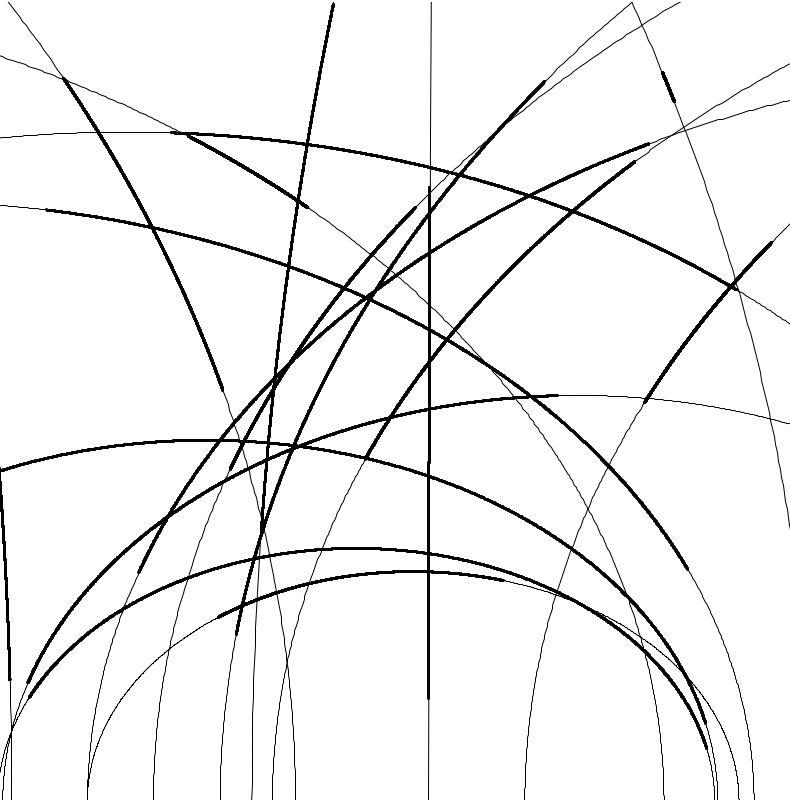
\includegraphics[width=0.4\textwidth]{FisherRaoGeodesics1D.png}  
%
\caption{Visualizing some Fisher–Rao geodesics of univariate normal distributions on the stretched Poincar\'e upper plane (semi-circles with origin on the $x$-axis and stretched by $\sqrt{2}$ on the $x$-axis). Full geodesics are plotted with a thin gray style and geodesic arcs are plotted with a thick black style.  
 \label{fig:vizgeo1d}}
\end{figure}

Notice that it is remarkable that the Fisher--Rao distance between normal distributions is available in closed form:
Indeed, the Euclidean length (with respect to the Euclidean metric) of semi-ellipse curves (perimeters) is not known in closed form but can be expressed using the so-called complete elliptic integral of the second kind~\cite{chandrupatla2010perimeter}.

 

%%%
\subsection{Geodesics with Initial Values on the Multivariate Fisher--Rao Normal~Manifold}
%%%
The geodesic equation is given by
$$
\left\{ \begin{array}{lcl}
\ddot\mu-\dot\Sigma\Sigma^{-1}\dot\mu &=& 0,\\
\ddot\Sigma+\dot\mu\dot\mu^\top-\dot\Sigma\Sigma^{-1}\dot\Sigma &=& 0.
\end{array}
\right.
$$

We concisely report the parametric geodesics using another variant of the natural parameters of the normal distributions (slightly differing from the $\theta$-coordinate system since natural parameters can be chosen up to a fixed affine transformation by changing accordingly the sufficient statistics by the inverse affine transformation) viewed as an exponential family:
$$
\left(\xi=\Sigma^{-1}\mu,\Xi=\Sigma^{-1}\right).
$$
In general, the~geodesics with boundary values $\gamma_\calN^\Fisher(N_1,N_2;t)$ are not known in closed form.
However, Calvo and Oller~\cite{calvo1991explicit} (Theorem~3.1 and Corollary~1) reported the explicit equations of the geodesics when the initial values are given, i.e.,~$\gamma_\calN^\Fisher(N_0,v_0;t)$ where $v_0=\dot\gamma_\calN^\Fisher(N_0,v_0;0)=(\dot\xi(0),\dot\Xi(0))$ is in $T_{N_0}\calM$ and $\gamma_\calN^\Fisher(N_0,v_0;0)=N_0$.


Let 
\begin{eqnarray*}
B &=& -\Xi(0)^{-\frac{1}{2}}\, \dot\Xi(0)\, \Xi(0)^{-\frac{1}{2}},\\
a &=& \Xi(0)^{-\frac{1}{2}}\dot\xi(0)+B\Xi_0^{-\frac{1}{2}}\xi(0),\\
G &=& (B^2+2aa^\top)^{\frac{1}{2}},
\end{eqnarray*}
and $G^\dagger$ be the Moore–Penrose generalized inverse matrix of $G$: $G^\dagger=(G^\top G)^{-1}G^\top$ or $G^\dagger=G^\top(G G^\top)^{-1}$. The~Moore–Penrose pseudo-inverse matrix can be replaced by any other pseudo-inverse matrix $G^-$~\cite{calvo1991explicit}.

Then we have $(\xi(t),\Xi(t))=\gamma_\calN^\Fisher(N_0,v_0;t)$ with
\begin{eqnarray*}
R(t)=\Cosh\left(\frac{1}{2} G  t\right) -BG^\dagger\Sinh\left(\frac{1}{2} G  t\right),\\
\Xi(t)=\Xi(0)^{\frac{1}{2}}\, R(t)R(t)^\top\, \Xi(0)^{\frac{1}{2}},\\
\xi(t)=2\Xi(0)^{\frac{1}{2}}\, R(t)\Sinh\left(\frac{1}{2} G  t\right)G^\dagger a+\Xi(t)\Xi^{-1}(0)\xi(0),
\end{eqnarray*}
where the Cosh and Sinh functions of a matrix $M$ are defined by the following absolutely convergent series~\cite{calvo1991explicit} ({Equation~(9),} %I confirm. MDPI: Please coinfirm Equation (9) belongs to Ref.48.
 p. 122):
\begin{eqnarray*}
\Sinh(M) &=& M +\sum_{i=1}^\infty \frac{M^{2i+1}}{(2i+1)!},\\
\Cosh(M) &=& I+ \sum_{i=1}^\infty \frac{M^{2i}}{(2i)!},
\end{eqnarray*}
and satisfies the identity $\Sinh^2(M)+\Cosh^2(M)=I$.
The matrix Cosh and Sinh functions can be calculated from the eigendecomposition of 
$M=O\, \diag(\lambda_1,\ldots,\lambda_d)\, O^\top$ as follows:

\begin{adjustwidth}{-\extralength}{0cm}
\centering %% If there is a figure in wide page, please release command \centering
\begin{eqnarray*}
\Sinh(M) &=& O\, \diag(\sinh(\lambda_1),\ldots,\sinh(\lambda_d))\, O^\top,\quad \sinh(u)=\frac{e^u-e^{-u}}{2}=
\sum_{i=0}^\infty \frac{u^{2i+1}}{(2i+1)!}, \\
\Cosh(M) &=& O\, \diag(\cosh(\lambda_1),\ldots,\cosh(\lambda_d))\, O^\top,\quad \cosh(u)=\frac{e^u+e^{-u}}{2}
=\sum_{i=0}^\infty \frac{u^{2i}}{(2i)!}.
\end{eqnarray*}
\end{adjustwidth}
 


When we restrict the manifold to a totally geodesic submanifold $\calM_\mu=\{P\succ 0\}$, 
the geodesic equation becomes $\ddot{P}-\dot{P}P^{-1}\dot{P}=0$, and~the
geodesic with initial values $P(0)=P$ and $\dot{P}(0)=S\in\Sym$ is:
$$
P(t)=P^{\frac{1}{2}}\, \exp\left(t P^{-\frac{1}{2}} S P^{-\frac{1}{2}}\right)\, P^{\frac{1}{2}}.
$$
The geodesic with boundary values   $P(0)=P_1$ and $P(1)=P_2$ is
$$
P(t)=P_1^{\frac{1}{2}}\, \exp\left(t \Log(P_1^{-\frac{1}{2}} P_2 P_1^{-\frac{1}{2}})\right)\, P_1^{\frac{1}{2}}.
$$
Furthermore, we can convert a geodesic with boundary values $\gamma_\bbP(P_1,P_2;t)$ to an equivalent geodesic with initial values
$\gamma_\bbP(P,S;t)$ by letting
$$
S= P_1^{\frac{1}{2}} \Log (P_1^{-\frac{1}{2}} P_2  P_1^{-\frac{1}{2}}) P_1^{\frac{1}{2}}.
$$


%%%
\section{Fisher–Rao Distance between Normal Distributions Sharing the Same Covariance~Matrix}\label{sec:BFRsamecovar}
%%%%

The Rao distance between $N_1=N(\mu_1,\Sigma)$ and $N_2=N(\mu_2,\Sigma)$ has been reported in closed form~\cite{FRMVNReview-2020} {(Proposition~3)}%Confirm! MDPI: Please confirm this Proposition belongs to Ref.42, if not, please add the link of it.
. We shall explain the geometric method in full as follows:
Let $(e_1,\ldots,e_d)$ be the standard frame of $\bbR^d$ (ordered basis): The $e_i$'s are the unit vectors of the axis $x_i$'s. 
Let $P$ be an orthogonal matrix such that $P\, (\mu_2-\mu_1)=\|\mu_2-\mu_1\|_2\, e_1$ 
(i.e., matrix $P$ aligns vector $\mu_2-\mu_1$ to the first axis $x_1$). Let $\Delta_{12}=\|\mu_2-\mu_1\|_2$ be the Euclidean distance between $\mu_1$ and $\mu_2$.
Furthermore, factorize matrix $P\Sigma P^\top$ using the LDL decomposition (a variant of the Cholesky decomposition) as 
$P\Sigma P^\top = LDL^\top$ where $L$ is a lower triangular matrix with all diagonal entries equal to one (lower unitriangular matrix of unit determinant) and $D$ a diagonal matrix. 
Let $\sigma_{12}=\sqrt{D_{11}}$.
Then we have~\cite{FRMVNReview-2020}:
\begin{equation}\label{eq:FRSigma}
\rho_\Sigma(\mu_1,\mu_2)= \rho_\calN(N(\mu_1,\Sigma),N(\mu_2,\Sigma)) = \rho_\calN(N(0,\sigma),N(\Delta_{12}e_1,\sigma_{12})).
\end{equation}
Please note that the right-hand side term is the Fisher–Rao distance between univariate normal distributions of Equation~(\ref{eq:FR1D}).

To find matrix $P$, we proceed as follows: Let $u=\frac{\mu_2-\mu_1}{\|\mu_2-\mu_1\|_2}$ be the normalized vector to align on axis $x_1$.
Let $v=u-e_1$. Consider the  Householder reflection matrix~\cite{householder1958unitary} $M=I-\frac{2vv^\top}{\|v\|_2^2}$, where $vv^\top$ is an outer product matrix.
Since Householder reflection matrices have determinant $-1$, we let $P$ be a copy of $M$ with the last row multiplied by $-1$ 
so that we obtain $\det(P)=1$. By~construction, we have $Pu=\|\mu_2-\mu_1\|_2\, e_1$.
We then use the affine-invariance property of the Fisher–Rao distance as follows:
\begin{eqnarray*}
\rho_\calN(N(\mu_1,\Sigma),N(\mu_2,\Sigma)) &=& \rho_\calN(N(0,\Sigma),N(\mu_2-\mu_1,\Sigma)),\\
&=& \rho_\calN(N(0,P\Sigma P^\top),N(P(\mu_2-\mu_1),P\Sigma P^\top)),\\
&=& \rho_\calN(N(0,P\Sigma P^\top),N(\Delta_{12}\, e_1,P\Sigma P^\top)),\\
&=& \rho_\calN(N(0,L D L^\top),N(\Delta_{12}\, e_1,L D L^\top)),\\
&=& \rho_\calN(N(0,D),N(\Delta_{12}\, e_1, D)).
\end{eqnarray*}
The last row follows from the fact that $L^{-1}e_1=e_1$ since $L^{-1}$ is an upper unitriangular matrix, and~
$L^\top (L^{-1})^\top=(L^{-1}L)^\top=I$.
The right-hand side Fisher–Rao distance is computed from Equation~(\ref{eq:FR1D}).



%%%
\section{Embedding the Set of Multivariate Normal Distributions in a Riemannian Symmetric~Space}\label{sec:SS}
%%%

The multivariate Gaussian manifold $\calN(d)$ can also be embedded into the SPD cone $\calP(d+1)$ as a Riemannian symmetric space~\cite{lovric2000multivariate,globke2021information}  by  $f_\SSPD$: $\hat\calP=\{f_\SSPD(N)\subset\calP(d+1)\ :\ N\in\calN(d)\}$.
We have $\hat\calP\cong\SL(d+1)/\SO(d+1)$~\cite{lovric2000multivariate,fernandes2000fisher,fernandes2003geometric} (and textbook~\cite{bridson2013metric}, Part II Chapter 10), and~the symmetric space $\SL(d+1)/\SO(d+1)$ can be embedded with the Killing Riemannian metric instead of the Fisher information metric:

\begin{adjustwidth}{-\extralength}{0cm}
\centering %% If there is a figure in wide page, please release command \centering
$$
g^\Killing(N_1,N_2)=\kappa_\Killing\, \left( \mu_1^\top\Sigma^{-1}\mu_2+\frac{1}{2}\tr\left(\Sigma^{-1}\Sigma_1\Sigma^{-1}\Sigma_2\right)
-\frac{1}{2(d+1)}\tr\left(\Sigma^{-1}\Sigma_1\right)\tr\left(\Sigma^{-1}\Sigma_2\right)\right), 
$$
\end{adjustwidth}
where $\kappa_\Killing>0$ is a predetermined constant (e.g., $1$).
The length element of the Killing metric is
$$
\ds_\SS^2=\kappa_\Killing\, \left(\frac{1}{2}\dmu^\top \Sigma^{-1} \dmu +\tr\left(\left(\Sigma^{-1}\dSigma\right)^2\right)-\frac{1}{2}\tr^2\left(\Sigma^{-1}\dSigma\right)\right).
$$
When we consider $\calN_\Sigma$, we may choose $\kappa_\Killing=2$ so that the Killing metric coincides with the Fisher information metric.
The induced Killing distance~\cite{lovric2000multivariate} is available in closed form:
\begin{equation}\label{eq:KillingDistance}
\rho_\Killing(N_1,N_2)=\sqrt {\kappa_\Killing\, \sum_{i=1}^{d+1} \log^2 \lambda_i\left(\hat{L}_1^{-1}\hat{P}_2\left(\hat{L}_1^{-1}\right)^\top\right)},
\end{equation}
where $\hat{L}_1$ is the unique lower triangular matrix obtained from the Cholesky decomposition of $\hat{P}_1=f_\SSPD(N_1)=\hat{L}_1\hat{L}_1^\top$.  
Please note that $\hat{L}_1^{-1}\hat{P}_2\left(\hat{L}_1^{-1}\right)^\top\in\calP(d+1)$ and $|\hat{L}_1|$, i.e.,~$\hat{L}_1\in\SL(d+1)$.

When $N_1=(\mu_1,\Sigma)$ and $N_2=(\mu_2,\Sigma)$ ($N_1,N_2\in\calN_\Sigma$), we have~\cite{lovric2000multivariate}
$$
\rho_\Killing(N_1,N_2)=\sqrt{2\kappa_\Killing}\arccosh\left(1+\frac{1}{2}\Delta_\Sigma^2(\mu_1,\mu_2)\right),
$$
where $\Delta_\Sigma^2$ is the squared Mahalanobis distance.
Thus, $\rho_\Killing(N_1,N_2)=h_\Killing(\Delta_\Sigma(\mu_1,\mu_2))$ where $h_\Killing(u)=\sqrt{2\kappa_\Killing}\arccosh\left(1+\frac{1}{2}u^2\right)$. 


When $N_1=(\mu,\Sigma_1)$ and $N_2=(\mu,\Sigma_2)$ ($N_1,N_2\in\calN_\mu$), we have~\cite{lovric2000multivariate}:

\begin{adjustwidth}{-\extralength}{0cm}
\centering %% If there is a figure in wide page, please release command \centering
\begin{eqnarray*}
\lefteqn{\rho_\Killing(N_1,N_2)=}\\
&& \sqrt{
\kappa_\Killing
\left(
\sum_{i=1}^d \log^2\lambda_i\left({L}_1^{-1}{P}_2\left({L}_1^{-1}\right)^\top\right)
-\frac{1}{(d+1)^2}
\left(\sum_{i=1}^d \log\lambda_i\left({L}_1^{-1}{P}_2\left({L}_1^{-1}\right)^\top\right)\right)
\right)
}.
\end{eqnarray*}
\end{adjustwidth}

%It is noticed in~\cite{lovric2000multivariate} that $\sum_{i=1}^{d+1} \log  \lambda_i\left(\hat{L}_1^{-1}\hat{P}_2\left(\hat{L}_1^{-1}\right)^\top\right)=0$.

See Example~\ref{ex1entropy}. Let us emphasize that the Killing distance is not the Fisher–Rao distance but is available in closed form as an alternative metric distance between~MVNs.

A Fisher geodesic defect measure of a curve $c$ is defined in~\cite{globke2021information} by 
$$
\delta(c)=\lim_{s\rightarrow \infty} \frac{1}{s}\int_0^s \|\nabla_{\dot{c}}^{g^\Fisher} \dot{c}\|_{c(t)}^\Fisher \dt,
$$
where $\nabla^{g^\Fisher}$ denotes the Levi–Civita connection induced by the Fisher metric. 
When $\delta(c)=0$ the curve is said to be an asymptotic geodesic of the Fisher geodesic.
It is proven that Killing geodesics at $(\mu,\Sigma)$ are asymptotic Fisher geodesics when the initial condition $c'(0)$ is orthogonal to $\calN_\mu$. 


%%%
\section{Embedding the Set of Multivariate Normal Distributions in the Siegel Upper~Space}\label{sec:Siegel}
%%%
The Siegel upper space is the space of symmetric complex matrices $Z=X+iY=Z^\top$ with imaginary positive–definite matrices $Y\succ 0$~\cite{siegel2014symplectic,nielsen2020siegel} (so-called Riemann matrices~\cite{frauendiener2019efficient}):
\begin{equation}
\SH(d) := \left\{ Z = X + iY \st X\in\Sym(d), Y\in\calP(d)\right\},
\end{equation}
where $\Sym(d)$ is the space of symmetric real $d\times d$ matrices.
$\SH(1)$ corresponds to the Poincar\'e upper plane.
See Figure~\ref{fig:SiegelDistance} for an~illustration.

The Siegel infinitesimal square line element is
\begin{equation}
\ds_\SH^2 (Z) = 2 \tr\left(Y^{-1}\dZ\ Y^{-1}\dZbar\right).
\end{equation}
When $X=0$ and $Z=iY$, we have $\dZ=i\dY$, $\dZbar=-i\dY$,  and~it follows that
$$
\ds_\SH^2 (iY)=2 \tr\left( (Y^{-1}\dY)^2\right).
$$
That is, four times the square length of the Fisher matrix of centered normal distributions 
$\ds^2_{\calN_0}=\frac{1}{2}\tr \left( (P^{-1}\dP)^2\right)$.

The  Siegel  distance~\cite{siegel2014symplectic} between $Z_1$ and $Z_2\in\SH(d)$ is
\begin{equation}\label{eq:SiegelDistance}
\rho_\SH(Z_1,Z_2) = \sqrt{\sum_{i=1}^d \log^2\left(\frac{1+\sqrt{r_i}}{1-\sqrt{r_i}}\right)},
\end{equation}
where
\begin{equation}
r_i=\lambda_i\left(R(Z_1,Z_2)\right),
\end{equation}
with $R(Z_1,Z_2)$ denoting  the matrix generalization of the {cross-ratio}
\begin{equation}\label{eq:matrixcr}
R(Z_1,Z_2)  := (Z_1-Z_2)(Z_1-\barZ_2)^{-1} (\barZ_1 -\barZ_2) (\barZ_1 -Z_2)^{-1},
\end{equation}
and $\lambda_i(M)$ denoting the $i$-th largest (real) eigenvalue of (complex) matrix $M$.
(In practice, we numerically must round off the tiny imaginary parts to obtain proper real eigenvalues~\cite{nielsen2020siegel}.)
The Siegel upper half space is a homogeneous space where the Lie Group $\mathrm{SU}(d,d)/S(U(d)\times U(d))$  acts transitively on~it.

 
We can embed a multivariate normal distribution $N=(\mu,\Sigma)$ into $\SH(d)$ as follows:
$$
N(\mu,\Sigma)\rightarrow Z(N):=\left(\mu\mu^\top+i\Sigma\right),
$$
and consider the Siegel distance on the embedded normal distributions as another potential metric distance between multivariate normal distributions:
\begin{equation}
\rho_\SH(N_1,N_2)=\rho_\SH(Z(N_1),Z(N_2)).
\end{equation}
Notice that the real matrix part of the $Z(N)$'s are all of rank one by~construction. 

\begin{figure}[H]

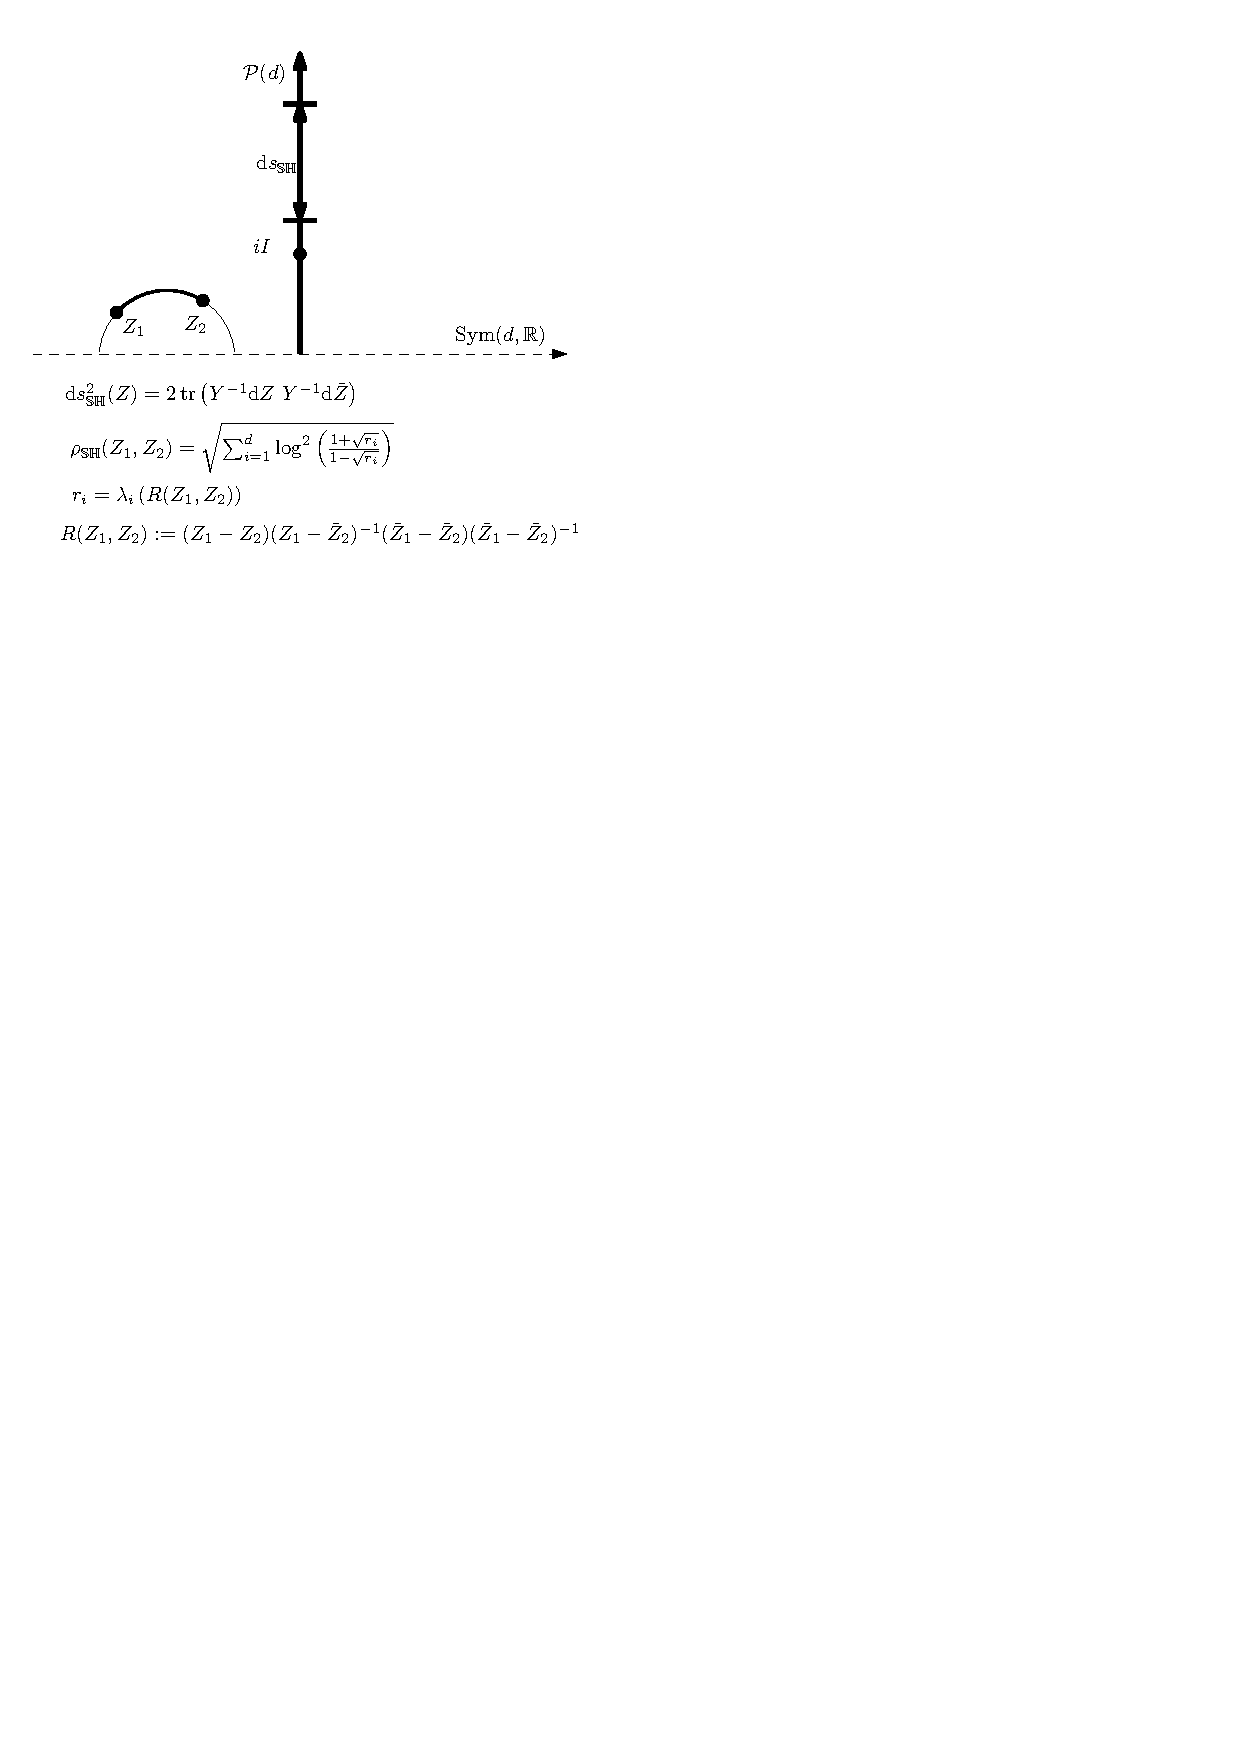
\includegraphics[width=0.55\textwidth]{FigIpe-MVNSiegelUpperDisk.pdf}
%
\caption{Siegel upper space generalizes the Poincar\'e hyperbolic upper plane.
 \label{fig:SiegelDistance}}
\end{figure}
\unskip

%%%
 \section{The Symmetrized Bregman Divergence Expressed as Integral Energies on Dual~Geodesics}\label{sec:proof}
%%%

Let $S_F(\theta_1;\theta_2)=B_F(\theta_1:\theta_2)+B_F(\theta_2:\theta_1)$ be a symmetrized Bregman divergence.
Let $\ds^2=\dtheta^\top \nabla^2 F(\theta)\dtheta$ denote the squared length element on the Bregman manifold 
and denote by $\gamma(t)$ and $\gamma^*(t)$ the dual geodesics connecting $\theta_1$ to $\theta_2$.
We can express $S_F(\theta_1;\theta_2)$ as integral energies on dual geodesics:
\begin{Property}
We have $S_F(\theta_1;\theta_2)=\int_0^1 \ds^2(\gamma(t))\dt=\int_0^1 \ds^2(\gamma^*(t))\dt$.
\end{Property}

\begin{proof}
The proof that the symmetrized Bregman divergence amount to these energy integrals
is based on the first-order and second-order directional derivatives.
The first-order directional derivative $\nabla_u F(\theta)$ with respect to vector $u$ is defined by 
$$
\nabla_u F(\theta)=\lim_{t\rightarrow 0} \frac{F(\theta+tv)-F(\theta)}{t}=v^\top \nabla F(\theta).
$$
 
The second-order directional derivatives $\nabla_{u,v}^2 F(\theta)$ is
\begin{eqnarray*}
\nabla_{u,v}^2 F(\theta) &=& \nabla_{u} \nabla_v F(\theta),\\
 &=& \lim_{t\rightarrow 0} \frac{v^\top \nabla F(\theta+tu)-v^\top\nabla F(\theta)}{t},\\
&=& u^\top \nabla^2 F(\theta) v.
\end{eqnarray*}


Now consider the squared length element $\ds^2(\gamma(t))$ on the primal geodesic $\gamma(t)$ expressed using the primal coordinate system $\theta$:
$\ds^2(\gamma(t))=\dtheta(t)^\top \nabla^2F(\theta(t)) \dtheta(t)$ with $\theta(\gamma(t))=\theta_1+t(\theta_2-\theta_1)$ and $\dtheta(t)=\theta_2-\theta_1$.
Let us express the $\ds^2(\gamma(t))$   using the second-order directional derivative:
$$
\ds^2(\gamma(t))=\nabla^2_{\theta_2-\theta_1}  F(\theta(t)).
$$
Thus, we have $\int_0^1 \ds^2(\gamma(t))\dt=[\nabla_{\theta_2-\theta_1}  F(\theta(t))]_0^1$,
where the first-order directional derivative is $\nabla_{\theta_2-\theta_1}  F(\theta(t))=(\theta_2-\theta_1)^\top \nabla F(\theta(t))$.
Therefore we obtain $\int_0^1 \ds^2(\gamma(t))\dt=(\theta_2-\theta_1)^\top (\nabla F(\theta_2)-\nabla F(\theta_1))=S_F(\theta_1;\theta_2)$.

Similarly, we express the squared length element $\ds^2(\gamma^*(t))$ using the dual coordinate system $\eta$ as the second-order directional derivative of $F^*(\eta(t))$ with $\eta(\gamma^*(t))=\eta_1+t(\eta_2-\eta_1)$:
$$
\ds^2(\gamma^*(t))=\nabla^2_{\eta_2-\eta_1}  F^*(\eta(t)).
$$
Therefore, we have  $\int_0^1 \ds^2(\gamma^*(t))\dt=[\nabla_{\eta_2-\eta_1}  F^*(\eta(t))]_0^1=S_{F^*}(\eta_1;\eta2)$.
Since $S_{F^*}(\eta_1;\eta_2)=S_F(\theta_1;\theta_2)$, we conclude that
$$
S_F(\theta_1;\theta_2)=\int_0^1 \ds^2(\gamma(t))\dt=\int_0^1 \ds^2(\gamma^*(t))\dt
$$

Please note that in 1D, both pregeodesics $\gamma(t)$ and $\gamma^*(t)$ coincide. We have $\ds^2(t)=(\theta_2-\theta_1)^2 f''(\theta(t))=(\eta_2-\eta_1){f^*}''(\eta(t))$ so that we check that $S_F(\theta_1;\theta_2)=\int_0^1 \ds^2(\gamma(t))\dt=(\theta_2-\theta_1)[f'(\theta(t))]_0^1=(\eta_2-\eta_1)[{f^*}'(\eta(t))]_0^1=(\eta_2-\eta_1)(\theta_2-\theta_2)$.
 \end{proof}
 


%%%%%%%%%%%%%%%%%%%%%%%%%%%%%%%%%%%%%%%%%%
\begin{adjustwidth}{-\extralength}{0cm}
%\printendnotes[custom] % Un-comment to print a list of endnotes

\reftitle{References}

% Please provide either the correct journal abbreviation (e.g. according to the “List of Title Word Abbreviations” http://www.issn.org/services/online-services/access-to-the-ltwa/) or the full name of the journal.
% Citations and References in Supplementary files are permitted provided that they also appear in the reference list here. 

%=====================================
% References, variant A: external bibliography
%=====================================
%\bibliography{your_external_BibTeX_file}

%=====================================
% References, variant B: internal bibliography
%=====================================

\begin{thebibliography}{999}

\bibitem[Amari(2016)]{IG-2016}
Amari, S.I.
\newblock {\em Information Geometry and Its Applications}; Applied Mathematical
  Sciences; Springer: {Japan, Tokyo} %MDPI: Please add the city of the publisher.
 2016.

\bibitem[Calin and Udri{\c{s}}te(2014)]{calin2014geometric}
Calin, O.; Udri{\c{s}}te, C.
\newblock {\em Geometric Modeling in Probability and Statistics}; 
  Springer: {Berlin/Heidelberg, Germany,} 2014; Volume 121.

\bibitem[Lin(2019)]{lin2019riemannian}
Lin, Z.
\newblock {Riemannian geometry of symmetric positive definite matrices via
  Cholesky decomposition}.
\newblock {\em SIAM J. Matrix Anal. Appl.} {\bf 2019},
  {\em 40},~1353--1370.

\bibitem[Soen and Sun(2021)]{soen2021variance}
Soen, A.; Sun, K.
\newblock {On the variance of the Fisher information for deep learning}.
\newblock {\em Adv. Neural Inf. Process. Syst.} {\bf 2021},
  {\em 34},~5708--5719.

\bibitem[Barachant \em{et~al.}(2013)Barachant, Bonnet, Congedo, and
  Jutten]{barachant2013classification}
Barachant, A.; Bonnet, S.; Congedo, M.; Jutten, C.
\newblock {Classification of covariance matrices using a Riemannian-based
  kernel for BCI applications}.
\newblock {\em Neurocomputing} {\bf 2013}, {\em 112},~172--178.

\bibitem[Skovgaard(1981)]{Skovgaard-1981}
Skovgaard, L.T.
\newblock {\em A Riemannian Geometry of the Multivariate Normal Model};
\newblock Technical Report 81/3; {{Statistical Research Unit, Danish Medical
  Research Council, Danish Social Science Research Council, Copenhagen, Denmark}%MDPI: Please add the location of the publisher (City and Country).
}:  1981.

\bibitem[Skovgaard(1984)]{Skovgaard-1984}
Skovgaard, L.T.
\newblock {A Riemannian geometry of the multivariate normal model}.
\newblock {\em Scand. J. Stat.} {\bf 1984}, \emph{{11}%confirm MDPI: Newly added information. Please confirm. the following highlights are the same
}, 211--223.

\bibitem[Malag{\`o} and Pistone(2015)]{malago2015information}
Malag{\`o}, L.; Pistone, G.
\newblock {Information geometry of the Gaussian distribution in view of
  stochastic optimization}.
\newblock In Proceedings of the ACM Conference on
  Foundations of Genetic Algorithms XIII, {Aberystwyth, UK, 17--22 January 2015}; pp. 150--162.

\bibitem[Herntier and Peter(2022)]{herntier2022transversality}
Herntier, T.; Peter, A.M.
\newblock {Transversality Conditions for Geodesics on the Statistical Manifold
  of Multivariate Gaussian Distributions}.
\newblock {\em Entropy} {\bf 2022}, {\em 24},~1698.

\bibitem[Atkinson and Mitchell(1981)]{AtkinsonRao-1981}
Atkinson, C.; Mitchell, A.F.
\newblock Rao's distance measure.
\newblock {\em Sankhy{\=A} Indian J. Stat. Ser.} {\bf
  1981}, \emph{{43}}, 345--365.

\bibitem[Radhakrishna~Rao(1945)]{Rao-1945}
Radhakrishna~Rao, C.
\newblock Information and accuracy attainable in the estimation of statistical
  parameters.
\newblock {\em Bull. Calcutta Math. Soc.} {\bf 1945}, {\em
  37},~81--91.

\bibitem[Chen \em{et~al.}(2021)Chen, Zhou, and Hu]{chen2021upper}
Chen, X.; Zhou, J.; Hu, S.
\newblock {Upper bounds for Rao distance on the manifold of multivariate
  elliptical distributions}.
\newblock {\em Automatica} {\bf 2021}, {\em 129},~109604.

\bibitem[Hotelling(1930)]{Hotelling-1930}
Hotelling, H.
\newblock Spaces of statistical parameters.
\newblock {\em Bull. Amer. Math. Soc} {\bf 1930}, {\em 36},~191.

\bibitem[Cencov(2000)]{cencov2000statistical}
Cencov, N.N.
\newblock {\em Statistical Decision Rules and Optimal Inference}; American
  Mathematical Soc.: {Providence, RI, USA,} 2000;
\newblock Volume~{53}% it is volume MDPI: Please check if it should be “Volume 53” or “p. 53”.
.

\bibitem[Bauer \em{et~al.}(2016)Bauer, Bruveris, and
  Michor]{bauer2016uniqueness}
Bauer, M.; Bruveris, M.; Michor, P.W.
\newblock Uniqueness of the Fisher--Rao metric on the space of smooth
  densities.
\newblock {\em Bull. Lond. Math. Soc.} {\bf 2016}, {\em
  48},~499--506.

\bibitem[Fujiwara(2022)]{fujiwara2022hommage}
Fujiwara, A.
\newblock {Hommage to Chentsov's theorem}.
\newblock {\em Inf. Geom.} {\bf 2022}, {1--20.} 
%There is no volume yet, it is online first https://link.springer.com/journal/41884/online-first MDPI: Please add the volume number.


\bibitem[Bruveris and Michor(2019)]{bruveris2019geometry}
Bruveris, M.; Michor, P.W.
\newblock {Geometry of the Fisher--Rao metric on the space of smooth densities
  on a compact manifold}.
\newblock {\em Math. Nachrichten} {\bf 2019}, {\em 292},~511--523.

\bibitem[Burbea and Oller~i Sala(1989)]{burbea1989rao}
Burbea, J.; Oller~i Sala, J.M.
\newblock {\em On Rao Distance Asymptotic Distribution};
\newblock {Technical Report Mathematics Preprint Series No. 67}; Universitat de
  Barcelona: {Barcelona, Spain,} 1989.

\bibitem[Calvo and Oller(1990)]{SDPMVN-1990}
Calvo, M.; Oller, J.M.
\newblock {A distance between multivariate normal distributions based in an
  embedding into the Siegel group}.
\newblock {\em J. Multivar. Anal.} {\bf 1990}, {\em
  35},~223--242.

\bibitem[Rios \em{et~al.}(1992)Rios, Villarroya, and Oller]{rios1992rao}
Rios, M.; Villarroya, A.; Oller, J.M.
\newblock Rao distance between multivariate linear normal models and their
  application to the classification of response curves.
\newblock {\em Comput. Stat. Data Anal.} {\bf 1992}, {\em
  13},~431--445.

\bibitem[Park and Kshirsagar(1994)]{park1994distances}
Park, P.S.; Kshirsagar, A.M.
\newblock Distances between normal populations when covariance matrices are
  unequal.
\newblock {\em Commun. Stat. Theory Methods} {\bf 1994},
  {\em 23},~3549--3556.

\bibitem[Gruber(2008)]{gruber2008some}
Gruber, M.H.
\newblock {Some applications of the Rao distance to shrinkage estimators}.
\newblock {\em Commun. Stat. Methods} {\bf 2008},
  {\em 37},~180--193.

\bibitem[Strapasson \em{et~al.}(2016)Strapasson, Pinele, and
  Costa]{strapasson2016clustering}
Strapasson, J.E.; Pinele, J.; Costa, S.I.
\newblock {Clustering using the Fisher-Rao distance}.
\newblock In Proceedings of the 2016 IEEE Sensor Array and Multichannel Signal
  Processing Workshop (SAM), {Rio de Janeiro, Brazil, 10--13 July 2016}; pp. 1--5.

\bibitem[Le~Brigant and Puechmorel(2019)]{le2019quantization}
Le~Brigant, A.; Puechmorel, S.
\newblock {Quantization and clustering on Riemannian manifolds with an
  application to air traffic analysis}.
\newblock {\em J. Multivar. Anal.} {\bf 2019}, {\em
  173},~685--703.

\bibitem[Said \em{et~al.}(2015)Said, Bombrun, and Berthoumieu]{said2015texture}
Said, S.; Bombrun, L.; Berthoumieu, Y.
\newblock {Texture classification using Rao's distance on the space of
  covariance matrices}.
\newblock In Proceedings of the Geometric Science of Information: Second
  International Conference, GSI 2015, Proceedings 2, Palaiseau, France, 28--30 October 2015;
   Springer: {Berlin/Heidelberg, Germany,} %newly added information, please confirm
  2015; pp. 371--378.

\bibitem[Legrand and Grivel(2016)]{legrand2016evaluating}
Legrand, L.; Grivel, E.
\newblock Evaluating dissimilarities between two moving-average models: A
  comparative study between Jeffrey's divergence and Rao distance.
\newblock In Proceedings of the 2016 24th European Signal Processing Conference
  (EUSIPCO), {Budapest, Hungary, 8 August--2 September 2016;} pp. 205--209.

\bibitem[Halder and Georgiou(2018)]{halder2018gradient}
Halder, A.; Georgiou, T.T.
\newblock {Gradient flows in filtering and Fisher-Rao geometry}.
\newblock In Proceedings of the 2018 Annual American Control Conference (ACC), {Milwaukee, WI, USA, 27--29 June
2018; }pp. 4281--4286.

\bibitem[Collas \em{et~al.}(2022)Collas, Breloy, Ren, Ginolhac, and
  Ovarlez]{collas2022riemannian}
Collas, A.; Breloy, A.; Ren, C.; Ginolhac, G.; Ovarlez, J.P.
\newblock {Riemannian optimization for non-centered mixture of scaled Gaussian
  distributions}.
\newblock {\em arXiv} {\bf 2022}, arXiv:2209.03315.

\bibitem[Liang \em{et~al.}(2019)Liang, Poggio, Rakhlin, and
  Stokes]{liang2019fisher}
Liang, T.; Poggio, T.; Rakhlin, A.; Stokes, J.
\newblock {Fisher-Rao metric, geometry, and complexity of neural networks}.
\newblock In Proceedings of the 22nd International Conference on Artificial
  Intelligence and Statistics, PMLR, {Naha, Japan, 16--18 April 2019;} pp. 888--896.

\bibitem[Yoshizawa and Tanabe(1999)]{IG-MVN-1999}
Yoshizawa, S.; Tanabe, K.
\newblock {Dual differential geometry associated with the Kullback-Leibler
  information on the Gaussian distributions and its $2$-parameter
  deformations}.
\newblock {\em SUT J. Math.} {\bf 1999}, {\em 35},~113--137.

\bibitem[Shima(2007)]{shima2007geometry}
Shima, H.
\newblock {\em {The Geometry of Hessian Structures}}; {World Scientific: Singapore} %OK! MDPI: Please add the location of the publisher (City and Country).
 2007.

\bibitem[Calvo and Oller(2002)]{SDPElliptical-2002}
Calvo, M.; Oller, J.M.
\newblock {A distance between elliptical distributions based in an embedding
  into the Siegel group}.
\newblock {\em J. Comput. Appl. Math.} {\bf 2002},
  {\em 145},~319--334.

\bibitem[Burbea(1984)]{burbea1984informative}
Burbea, J.
\newblock\emph{ Informative Geometry of Probability Spaces};
\newblock Technical Report; {Pittsburgh Univ. PA Center for Multivariate
  Analysis: Pittsburgh, USA} %OK! MDPI: Please add the location of the publisher (City and Country).
1984.

\bibitem[Eriksen(1986)]{Eriksen-1986}
Eriksen, P.S.
\newblock {\em Geodesics Connected with the Fischer Metric on the Multivariate
  Normal Manifold}; {Institute of Electronic Systems, Aalborg University Centre: Aalborg, Denmark}%OK! MDPI: Please add the location of the publisher (City and Country).
   1986.

\bibitem[Berkane \em{et~al.}(1997)Berkane, Oden, and
  Bentler]{FRGeodesicEll-1997}
Berkane, M.; Oden, K.; Bentler, P.M.
\newblock Geodesic estimation in elliptical distributions.
\newblock {\em J. Multivar. Anal.} {\bf 1997}, {\em 63},~35--46.

\bibitem[Imai \em{et~al.}(2011)Imai, Takaesu, and Wakayama]{imai2011remarks}
Imai, T.; Takaesu, A.; Wakayama, M.
\newblock \emph{Remarks on Geodesics for Multivariate Normal Models};
\newblock Technical Report; {Faculty of Mathematics, Kyushu University: Fukuoka, Japan}  2011.%OK! MDPI: Please add the location of the publisher (City and Country).
% https://catalog.lib.kyushu-u.ac.jp/opac_download_md/20147/JMI2011B-6.pdf

\bibitem[Inoue(2015)]{inoue2015group}
Inoue, H.
\newblock Group theoretical study on geodesics for the elliptical models.
\newblock In Proceedings of the Geometric Science of Information: Second
  International Conference, GSI 2015, Proceedings 2, Palaiseau, France, 28--30 October 2015;
  Springer: {Berlin/Heidelberg, Germany,} %newly added information, please confirm
 2015; pp. 605--614.

\bibitem[Strapasson \em{et~al.}(2015)Strapasson, Porto, and
  Costa]{strapasson2015bounds}
Strapasson, J.E.; Porto, J.P.; Costa, S.I.
\newblock {On bounds for the Fisher-Rao distance between multivariate normal
  distributions}.
\newblock {\em AIP Conf. Proc.} {\bf 2015}, {\em 1641},~313--320.

\bibitem[Han and Park(2014)]{MVNGeodesicShooting-2014}
Han, M.; Park, F.C.
\newblock {DTI segmentation and fiber tracking using metrics on multivariate
  normal distributions}.
\newblock {\em J. Math. Imaging Vis.} {\bf 2014}, {\em
  49},~317--334.

\bibitem[Pilt{\'e} and Barbaresco(2016)]{GeodesicShooting-2016}
Pilt{\'e}, M.; Barbaresco, F.
\newblock Tracking quality monitoring based on information geometry and
  geodesic shooting.
\newblock In Proceedings of the 2016 17th International Radar Symposium (IRS), {Krakow, Poland, 10--12 May 2016;} pp. 1--6.

\bibitem[Barbaresco(2019)]{barbaresco2019souriau}
Barbaresco, F.
\newblock {Souriau exponential map algorithm for machine learning on matrix Lie
  groups}.
\newblock In Proceedings of the Geometric Science of Information: 4th
  International Conference, GSI 2019, Proceedings 4, Toulouse, France, 27--29 August 2019;
  Springer: {Berlin/Heidelberg, Germany,} %We added the location of publisher. Please confirm
  2019; pp. 85--95.

\bibitem[Pinele \em{et~al.}(2020)Pinele, Strapasson, and
  Costa]{FRMVNReview-2020}
Pinele, J.; Strapasson, J.E.; Costa, S.I.
\newblock {The Fisher--Rao distance between multivariate normal distributions:
  Special cases, bounds and applications}.
\newblock {\em Entropy} {\bf 2020}, {\em 22},~404.

\bibitem[Dijkstra(2022)]{dijkstra2022note}
Dijkstra, E.W.
\newblock A note on two problems in connexion with graphs. In {\em {Edsger Wybe
  Dijkstra: His Life, Work, and Legacy}}; {Association for Computing Machinery: New York City, USA} %OK! MDPI: Please add the location of the publisher (City and Country).
  2022; pp. 287--290.

\bibitem[Anderson(2006)]{anderson2006hyperbolic}
Anderson, J.W.
\newblock {\em Hyperbolic Geometry}; Springer Science \& Business Media: {Berlin/Heidelberg, Germany,} %We added the location of publisher. Please confirm
   2006.

\bibitem[Siegel(2014)]{siegel2014symplectic}
Siegel, C.L.
\newblock {\em Symplectic Geometry}; first printed in 1964; Elsevier: {Amsterdam, The Netherlands,} %We added the location of publisher. Please confirm
  2014.


\bibitem[James(1973)]{DoubleCone-James-1973}
James, A.T.
\newblock The variance information manifold and the functions on it. In {\em
  Multivariate Analysis--III}; Elsevier: {Amsterdam, The Netherlands,} %We added the location of publisher. Please confirm
   1973; pp. 157--169.

\bibitem[Wells \em{et~al.}(2020)Wells, Cook, Pine, and
  Robinson]{wells2020fisher}
Wells, J.; Cook, M.; Pine, K.; Robinson, B.D.
\newblock {Fisher-Rao distance on the covariance cone}.
\newblock {\em arXiv} {\bf 2020}, arXiv:2010.15861.

\bibitem[Calvo and Oller(1991)]{calvo1991explicit}
Calvo, M.; Oller, J.M.
\newblock An explicit solution of information geodesic equations for the
  multivariate normal model.
\newblock {\em Stat. Risk Model.} {\bf 1991}, {\em 9},~119--138.

\bibitem[F{\"o}rstner and Moonen(2003)]{forstner2003metric}
F{\"o}rstner, W.; Moonen, B.
\newblock A metric for covariance matrices.
\newblock {In \em Geodesy-the Challenge of the 3rd Millennium}; Springer: Berlin/Heidelberg, Germany, {\bf 2003};~299--309.




\bibitem[Dolcetti and Pertici(2020)]{dolcetti2020real}
Dolcetti, A.; Pertici, D.
\newblock Real square roots of matrices: Differential properties in
  semi-simple, symmetric and orthogonal cases.
\newblock 
 \emph{arXiv}, \textbf{2020}, {arXiv}:2010.15609.

% https://www.springer.com/journal/43538
\bibitem[Mahalanobis(1936)]{mahalanobis1936generalised}
Mahalanobis, P.C.
\newblock On the generalised distance in statistics.
\newblock In \emph{Proceedings of the National Institute of
  Science of India},  Springer: New Delhi, India ; {1936;} %done MDPI: Please add the name of the publisher and their location.
 Volume~12, pp. 49--55.

\bibitem[Eaton(1989)]{eaton1989group}
Eaton, M.L.
\newblock {\em Group Invariance Applications in Statistics}; {Institute of
  Mathematical Statistics: Beachwood, Ohio, United States} %Done! MDPI: Please add the location of the publisher.
  1989.

 

\bibitem[Godinho and Nat{\'a}rio(2012)]{godinho2012introduction}
Godinho, L.; Nat{\'a}rio, J.
\newblock {An introduction to Riemannian geometry: With Applications to Mechanics and Relativity}.
\newblock {In \em Universitext}; Springer International Publishing: Cham, Switzerland, {2014}.

 

\bibitem[Strapasson \em{et~al.}(2016)Strapasson, Pinele, and
  Costa]{strapasson2016totally}
Strapasson, J.E.; Pinele, J.; Costa, S.I.
\newblock {A totally geodesic submanifold of the multivariate normal
  distributions and bounds for the Fisher-Rao distance}.
\newblock In Proceedings of the IEEE Information Theory Workshop (ITW), {Cambridge, UK, 1--11 September 2016;}
  \mbox{pp. 61--65.}

\bibitem[Chen and Zhou(2022)]{chen2022multisensor}
Chen, X.; Zhou, J.
\newblock Multisensor Estimation Fusion on Statistical Manifold.
\newblock {\em Entropy} {\bf 2022}, {\em 24},~1802.

\bibitem[Cherian and Sra(2016)]{Sra-2016}
Cherian, A.; Sra, S.
\newblock Riemannian dictionary learning and sparse coding for positive
  definite matrices.
\newblock {\em IEEE Trans. Neural Networks Learn. Syst.} {\bf
  2016}, {\em 28},~2859--2871.

\bibitem[Nguyen(2021)]{nguyen2021geomnet}
Nguyen, X.S.
\newblock {Geomnet: A neural network based on Riemannian geometries of SPD
  matrix space and Cholesky space for 3d skeleton-based interaction
  recognition}.
\newblock In Proceedings of the IEEE/CVF International
  Conference on Computer Vision, {Montreal, BC, Canada, 11--17 October 2021}; pp. 13379--13389.

\bibitem[Dolcetti and Pertici(2018)]{SPDisometries-2018}
Dolcetti, A.; Pertici, D.
\newblock Differential properties of spaces of symmetric real matrices.
\emph{arXiv} \textbf{2018}, arXiv:1807.01113.

\bibitem[Verdoolaege and Scheunders(2012)]{verdoolaege2012geometry}
Verdoolaege, G.; Scheunders, P.
\newblock {On the geometry of multivariate generalized Gaussian models}.
\newblock {\em J. Math. Imaging Vis.} {\bf 2012}, {\em
  43},~180--193.

\bibitem[Ali and Silvey(1966)]{fdiv-AliSilvey-1966}
Ali, S.M.; Silvey, S.D.
\newblock A general class of coefficients of divergence of one distribution
  from another.
\newblock {\em J. R. Stat. Soc. Ser. B} {\bf 1966}, {\em 28},~131--142.

\bibitem[Csisz{\'a}r(1967)]{Csiszar-1967}
Csisz{\'a}r, I.
\newblock Information-type measures of difference of probability distributions
  and indirect observation.
\newblock {\em Stud. Sci. Math. Hung.} {\bf 1967}, {\em
  2},~229--318.

\bibitem[Nielsen and Okamura(2022)]{nielsen2022note}
Nielsen, F.; Okamura, K.
\newblock A note on the $f$-divergences between multivariate location-scale
  families with either prescribed scale matrices or location parameters.
\newblock {\em arXiv} {\bf 2022}, arXiv:2204.10952.

\bibitem[Moakher and Z{\'e}ra{\"\i}(2011)]{moakher2011riemannian}
Moakher, M.; Z{\'e}ra{\"\i}, M.
\newblock {The Riemannian geometry of the space of positive-definite matrices
  and its application to the regularization of positive-definite matrix-valued
  data}.
\newblock {\em J. Math. Imaging Vis.} {\bf 2011}, {\em
  40},~171--187.

\bibitem[Dolcetti and Pertici(2021)]{EllipticIsometrySPD-2021}
Dolcetti, A.; Pertici, D.
\newblock Elliptic isometries of the manifold of positive definite real
  matrices with the trace metric.
\newblock {\em Rend. Del Circ. Mat. Di Palermo Ser. 2} {\bf
  2021}, {\em 70},~575--592.

\bibitem[Nielsen(2020)]{nielsen2020siegel}
Nielsen, F.
\newblock {The Siegel--Klein Disk: Hilbert Geometry of the Siegel Disk Domain}.
\newblock {\em Entropy} {\bf 2020}, {\em 22},~1019.

\bibitem[Arnaudon and Nielsen(2013)]{RieMinimax-2013}
Arnaudon, M.; Nielsen, F.
\newblock {On approximating the Riemannian $1$-center}.
\newblock {\em Comput. Geom.} {\bf 2013}, {\em 46},~93--104.

\bibitem[Ceolin and Hancock(2012)]{ceolin2012computing}
Ceolin, S.R.; Hancock, E.R.
\newblock {Computing gender difference using Fisher-Rao metric from facial
  surface normals}.
\newblock In Proceedings of the 25th SIBGRAPI Conference on Graphics, Patterns
  and Images, {Ouro Preto, Brazil, 22--25 August 2012;} pp. 336--343.

\bibitem[Wang \em{et~al.}(2017)Wang, Li, and Zhang]{wang2017g2denet}
Wang, Q.; Li, P.; Zhang, L.
\newblock G2DeNet: Global Gaussian distribution embedding network and its
  application to visual recognition.
\newblock In Proceedings of the IEEE Conference on Computer
  Vision and Pattern Recognition, { Honolulu, HI, USA, 21--26 July 2017;} \mbox{pp. 2730--2739}.

\bibitem[Miyamoto \em{et~al.}(2022)Miyamoto, Meneghetti, and
  Costa]{miyamoto2022fisher}
Miyamoto, H.K.; Meneghetti, F.C.; Costa, S.I.
\newblock {The Fisher--Rao loss for learning under label noise}.
\newblock {\em Inf. Geom.} {\bf 2022}, {1--20.} %No volume number yet, it is online first. MDPI: Please add the volume number.
% https://link.springer.com/article/10.1007/s41884-022-00076-8

\bibitem[Kurtek and Bharath(2015)]{kurtek2015bayesian}
Kurtek, S.; Bharath, K.
\newblock {Bayesian sensitivity analysis with the Fisher--Rao metric}.
\newblock {\em Biometrika} {\bf 2015}, {\em 102},~601--616.

\bibitem[Marti \em{et~al.}(2016)Marti, Andler, Nielsen, and
  Donnat]{marti2016optimal}
Marti, G.; Andler, S.; Nielsen, F.; Donnat, P.
\newblock {Optimal transport vs. Fisher-Rao distance between copulas for
  clustering multivariate time series}.
\newblock In Proceedings of the 2016 IEEE Statistical Signal Processing
  Workshop (SSP), {Palma de Mallorca, Spain, 26--29 June 2016;} pp. 1--5.

\bibitem[Tang \em{et~al.}(2018)Tang, Rong, Zhou, and Li]{tang2018information}
Tang, M.; Rong, Y.; Zhou, J.; Li, X.R.
\newblock Information geometric approach to multisensor estimation fusion.
\newblock {\em IEEE Trans. Signal Process.} {\bf 2018}, {\em
  67},~279--292.

\bibitem[Wang \em{et~al.}(2015)Wang, Wang, Huang, Shan, and
  Chen]{DA-FisherRaoMVN-2015}
Wang, W.; Wang, R.; Huang, Z.; Shan, S.; Chen, X.
\newblock {Discriminant analysis on Riemannian manifold of Gaussian
  distributions for face recognition with image sets}.
\newblock In Proceedings of the IEEE Conference on Computer
  Vision and Pattern Recognition, {Boston, MA, USA}, {7--12 June 2015}; pp. 2048--2057.

\bibitem[Li \em{et~al.}(2016)Li, Wang, Zeng, and Zhang]{li2016local}
Li, P.; Wang, Q.; Zeng, H.; Zhang, L.
\newblock {Local log-Euclidean multivariate Gaussian descriptor and its
  application to image classification}.
\newblock {\em IEEE Trans. Pattern Anal. Mach. Intell.}
  {\bf 2016}, {\em 39},~803--817.

\bibitem[Picot \em{et~al.}(2022)Picot, Messina, Boudiaf, Labeau, Ayed, and
  Piantanida]{picot2022adversarial}
Picot, M.; Messina, F.; Boudiaf, M.; Labeau, F.; Ayed, I.B.; Piantanida, P.
\newblock {Adversarial robustness via Fisher-Rao regularization}.
\newblock {\em IEEE Trans. Pattern Anal. Mach. Intell.}
  \bf {2022}, {\em 45}(3),~ 2698--2710 

 

\bibitem[Collas \em{et~al.}(2022)Collas, Bouchard, Ginolhac, Breloy, Ren, and
  Ovarlez]{collas2022use}
Collas, A.; Bouchard, F.; Ginolhac, G.; Breloy, A.; Ren, C.; Ovarlez, J.P.
\newblock {On the Use of Geodesic Triangles between Gaussian Distributions for
  Classification Problems}.
\newblock In Proceedings of the IEEE International Conference on Acoustics,
  Speech and Signal Processing (ICASSP), {Singapore, 22--27 May 2022;} pp. 5697--5701.

\bibitem[Murena \em{et~al.}(2018)Murena, Cornu{\'e}jols, and
  Dessalles]{murena2018opening}
Murena, P.A.; Cornu{\'e}jols, A.; Dessalles, J.L.
\newblock Opening the parallelogram: Considerations on non-Euclidean analogies.
\newblock In Proceedings of the Case-Based Reasoning Research and Development:
  26th International Conference, ICCBR 2018, Proceedings 26, Stockholm, Sweden, 9--12 July 2018; Springer: {Berlin/Heidelberg, Germany,} %We added the location of publisher. Please confirm
2018; pp. 597--611.

\bibitem[Popovi{\'c} \em{et~al.}(2022)Popovi{\'c}, Janev, Krstanovi{\'c},
  Simi{\'c}, and Deli{\'c}]{popovic2022measure}
Popovi{\'c}, B.; Janev, M.; Krstanovi{\'c}, L.; Simi{\'c}, N.; Deli{\'c}, V.
\newblock {Measure of Similarity between GMMs Based on Geometry-Aware
  Dimensionality Reduction}.
\newblock {\em Mathematics} {\bf 2022}, {\em 11},~175.

\bibitem[Micchelli and Noakes(2005)]{micchelli2005rao}
Micchelli, C.A.; Noakes, L.
\newblock Rao distances.
\newblock {\em J. Multivar. Anal.} {\bf 2005}, {\em 92},~97--115.

\bibitem[Nielsen(2019)]{nielsen2019jensen}
Nielsen, F.
\newblock {On the Jensen--Shannon symmetrization of distances relying on
  abstract means}.
\newblock {\em Entropy} {\bf 2019}, {\em 21},~485.

\bibitem[Davis and Dhillon(2006)]{davis2006differential}
Davis, J.; Dhillon, I.
\newblock {Differential entropic clustering of multivariate Gaussians}.
\newblock {\em Adv. Neural Inf. Process. Syst.} {\bf 2006},
  {\em 19},~337--344.

\bibitem[Welzl(2005)]{welzl2005smallest}
Welzl, E.
\newblock Smallest enclosing disks (balls and ellipsoids).
\newblock In \emph{Proceedings of the New Results and New Trends in Computer Science};
  Springer: {Berlin/Heidelberg, Germany,} %newly added information, please confirm
  2005; pp. 359--370.

\bibitem[Gonzalez(1985)]{gonzalez1985clustering}
Gonzalez, T.F.
\newblock Clustering to minimize the maximum intercluster distance.
\newblock {\em Theor. Comput. Sci.} {\bf 1985}, {\em 38},~293--306.

\bibitem[Acharyya \em{et~al.}(2013)Acharyya, Banerjee, and
  Boley]{acharyya2013bregman}
Acharyya, S.; Banerjee, A.; Boley, D.
\newblock Bregman divergences and triangle inequality.
\newblock In Proceedings of the 2013 SIAM International
  Conference on Data Mining, SIAM, {Austin, TX, USA, 2--4 May 2013;} pp. 476--484.

\bibitem[Lovri{\'c} \em{et~al.}(2000)Lovri{\'c}, Min-Oo, and
  Ruh]{lovric2000multivariate}
Lovri{\'c}, M.; Min-Oo, M.; Ruh, E.A.
\newblock {Multivariate normal distributions parametrized as a Riemannian
  symmetric space}.
\newblock {\em J. Multivar. Anal.} {\bf 2000}, {\em 74},~36--48.

\bibitem[Ohara \em{et~al.}(1996)Ohara, Suda, and Amari]{ohara1996dualistic}
Ohara, A.; Suda, N.; Amari, S.i.
\newblock Dualistic differential geometry of positive definite matrices and its
  applications to related problems.
\newblock {\em Linear Algebra Its Appl.} {\bf 1996}, {\em
  247},~31--53.

\bibitem[Nock and Nielsen(2005)]{BBC-2005}
Nock, R.; Nielsen, F.
\newblock {Fitting the smallest enclosing Bregman ball}.
\newblock In Proceedings of the Machine Learning: ECML 2005: 16th European
  Conference on Machine Learning, Proceedings 16, Porto, Portugal, 3--7 October 2005;
   Springer: {Berlin/Heidelberg, Germany,} 2005; pp. 649--656.

\bibitem[Ohara(2019)]{ohara2019doubly}
Ohara, A.
\newblock Doubly autoparallel structure on positive definite matrices and its
  applications.
\newblock In Proceedings of the International Conference on Geometric Science
  of Information, {Toulouse, France, 27--29 August 2019}; Springer: {Berlin/Heidelberg, Germany,} 
  2019; pp. 251--260.

\bibitem[Globke and Quiroga-Barranco(2021)]{globke2021information}
Globke, W.; Quiroga-Barranco, R.
\newblock Information geometry and asymptotic geodesics on the space of normal
  distributions.
\newblock {\em Inf. Geom.} {\bf 2021}, {\em 4},~131--153.

\bibitem[Nielsen and Sun(2019)]{nielsen2019clustering}
Nielsen, F.; Sun, K.
\newblock {Clustering in Hilbert's projective geometry: The case studies of the
  probability simplex and the elliptope of correlation matrices}.
\newblock {In \em Geometric Structures of Information}; Springer: {Berlin/Heidelberg, Germany,}  {\bf 2019}; pp. 297--331.
 


\bibitem[Journ{\'e}e \em{et~al.}(2010)Journ{\'e}e, Nesterov, Richt{\'a}rik, and
  Sepulchre]{journee2010generalized}
Journ{\'e}e, M.; Nesterov, Y.; Richt{\'a}rik, P.; Sepulchre, R.
\newblock Generalized power method for sparse principal component analysis.
\newblock {\em J. Mach. Learn. Res.} {\bf 2010}, {\em 11}, {517--553.} %OK! confirmed. MDPI: Newly added information. Please confirm.


\bibitem[Verdoolaege(2015)]{verdoolaege2015new}
Verdoolaege, G.
\newblock A new robust regression method based on minimization of geodesic
  distances on a probabilistic manifold: Application to power laws.
\newblock {\em Entropy} {\bf 2015}, {\em 17},~4602--4626.

\bibitem[Chandrupatla and Osler(2010)]{chandrupatla2010perimeter}
Chandrupatla, T.R.; Osler, T.J.
\newblock The perimeter of an ellipse.
\newblock {\em Math. Sci.} {\bf 2010}, {\em 35}.

\bibitem[Householder(1958)]{householder1958unitary}
Householder, A.S.
\newblock Unitary triangularization of a nonsymmetric matrix.
\newblock {\em J. ACM} {\bf 1958}, {\em 5},~339--342.

\bibitem[Fernandes and San~Martin(2000)]{fernandes2000fisher}
Fernandes, M.A.; San~Martin, L.A.
\newblock Fisher information and $\alpha$-connections for a class of
  transformational models.
\newblock {\em Differ. Geom. Its Appl.} {\bf 2000}, {\em
  12},~165--184.

\bibitem[Fernandes and San~Martin(2003)]{fernandes2003geometric}
Fernandes, M.A.; San~Martin, L.A.
\newblock {Geometric proprieties of invariant connections on
  $\mathrm{SL}(n,R)/\mathrm{SO}(n)$}.
\newblock {\em J. Geom. Phys.} {\bf 2003}, {\em 47},~369--377.

\bibitem[Bridson and Haefliger(2013)]{bridson2013metric}
Bridson, M.R.; Haefliger, A.
\newblock {\em Metric Spaces of Non-Positive Curvature}; Springer
  Science \& Business Media:  {Berlin/Heidelberg, Germany,} %Confirmed. thanks! We added the location of publisher. Please confirm
 2013; Volume 319.

\bibitem[Frauendiener \em{et~al.}(2019)Frauendiener, Jaber, and
  Klein]{frauendiener2019efficient}
Frauendiener, J.; Jaber, C.; Klein, C.
\newblock Efficient computation of multidimensional theta functions.
\newblock {\em J. Geom. Phys.} {\bf 2019}, {\em
  141},~147--158.

\end{thebibliography}

 
\PublishersNote{}
\end{adjustwidth}
\end{document}
